\ProvidesFile{template.tex}
    [2013/04/16 v3.2013^^J%
     Template file for NDdiss2e class by Sameer Vijay and updated by Megan Patnott^^J]
\documentclass[noinfo,final,sort&compress]{nddiss2e}
% One of the options draft, review, final must be chosen.
% One of the options textrefs or numrefs should be chosen
% to specify if you want numerical or ``author-date''
% style citations.
% Other available options are:
% 10pt/11pt/12pt (available with draft only)
% twoadvisors
% noinfo (should be used when you compile the final time
%         for formal submission)
% sort (sorts multiple citations in the order that they're
%       listed in the bibliography)
% compress (compresses numerical citations, e.g. [1,2,3]
%           becomes [1-3]; has no effect when used with
%           the textrefs option)
% sort&compress (sorts and compresses numerical citations;
%           is identical to sort when used with textrefs)

% \usepackage{amsmath}
% % \usepackage{amssymb}
% \usepackage{graphicx}
% \usepackage{multirow}
% \usepackage{dcolumn}
%\usepackage{bm} 
% \usepackage{amssymb}
%\usepackage{tablefootnote}
% \usepackage{times}
% \usepackage{mathptm}
%\usepackage{caption}
% \usepackage{float}
% \usepackage{geometry}
% \usepackage{xkeyval}
% \usepackage{tabularx}
% \usepackage{longtable}
% \usepackage{multicol}
% \usepackage{square}{natbib}
% \usepackage{achemso}
% \usepackage{cleveref}
%----my packs--
\usepackage{tikz}
\usetikzlibrary{shapes,arrows}
\usepackage{pdflscape}
\usepackage[version=3]{mhchem}
\usepackage{mathtools}
\usepackage{abraces}
\usepackage{threeparttable}
\usepackage{multirow}
\usepackage{dcolumn}
\usepackage[export]{adjustbox}
\usepackage{mathrsfs}
\usepackage{ragged2e}
\usepackage{csquotes}
%----my packs--

% \usepackage{tikz}
% \usetikzlibrary{shapes,arrows}
% \usepackage{pdflscape}
% \usepackage[version=3]{mhchem}
% \usepackage{mathtools}
% \usepackage{abraces}
% \usepackage{threeparttable}

%\setcitestyle{square}

%\newcommand*{\citen}[1]{%
 % \begingroup
  %  \romannumeral-`\x % remove space at the beginning of \setcitestyle
   % \setcitestyle{numbers}%
   % \cite{#1}%
  %\endgroup   
%}

\newcommand{\degree}{\ensuremath{^\circ}}

\begin{document}

\frontmatter % All the items before the first chapter go in ``frontmatter''

\title{DISCOVERING THE MOLECULAR ORIGINS OF SOLID-LIQUID FRICTION AT 
  ICE-I$_\mathrm{h}$/WATER INTERFACES}
\author{Patrick B. Louden}
\work{Dissertation}
\degaward{Doctor of Philosophy}
\advisor{J. Daniel Gezelter}
\department{Chemistry and Biochemstry}
\maketitle
%%%%%%%%%%%%%%%%%%%%%%%%%%%%%%%%%%%%%%%%%%%%%%%%%%%%%%%%%%%%%%%%%%%%%%%%%%%%%%%%%%%
%		FRONT STUFF
%%%%%%%%%%%%%%%%%%%%%%%%%%%%%%%%%%%%%%%%%%%%%%%%%%%%%%%%%%%%%%%%%%%%%%%%%%%%%%%%%%%

%\copyrightholder{Patrick B. Louden} 
%\copyrightyear{2017}           
%\makecopyright

\begin{abstract}
  In this dissertation I present work on the modeling of hydrodynamic
  friction at the surface of ice. In the hydrodynamic regime, a slider
  traversing an ice surface is fully supported by a
  quasi-liquid layer (QLL), and the resulting friciton is comprised of
  three parts; solid-liquid friction between the ice crystal and the
  QLL, viscous shearing of the surface premelt, and the drag force due
  to capillary bridges forming between the QLL and the slider.

  Using non-equilibrium molecular dynamics simulations, the basal
  $\{0001\}$, prismatic $\{10\bar{1}0\}$, 14\degree~pyramidal
  $\{20\bar{2}1\}$, and secondary prismatic $\{11\bar{2}0\}$ facets of
  ice-I$_\mathrm{h}$ were drawn through liquid water with a momentum
  flux between the solid and liquid phases. The spatial transition
  between the ice and the liquid was quantified using structural and
  dynamic order parameters. Estimates of the interfacial width using
  structural measures gave widths of $\sim$ 6-10~\AA. Dynamic
  interfacial widths were quantified and predicted a slightly broader
  interface, $\sim$~10-15~\AA~ wide. In addition, spatial
  decomposition of molecular orientational correlation functions
  indicated that the short- and longer-time decay components behave
  differently closer to the interface. In all cases the interface was
  observed to be stable under the presence of a shear.

  Water sliding over the surface of ice is observed to be in the
  no-slip limit. A friction coefficient appropriate for negative slip
  boundary conditions is presented, and crystal facet dependent
  friction is observed. The computed friction of these interfaces is
  found to be invariant to the shear rate and direction of shear
  relative to the surface features. This trend is observed for two
  water potentials, and is shown to correlate strongly with the
  surface hydrogen-bond density. A momentum transmission model is
  proposed, which relates the observed friction with the density of
  solid to liquid hydrogen bonds, the shear viscosity of the liquid,
  and the width of the interface. Data collected from both models
  agrees well with the proposed model.

  A temperature dependence study of the surface premelt at the basal
  and prismatic facets of an ice-I$_\mathrm{h}$ crystal is
  presented. Spatially resolved diffusion constants are computed
  normal to the ice surface, and estimates of the shear viscosity for
  the QLLs are obtained. A facet depedence is observed in the shear
  viscosity which correlates strongly with the computed solid-liquid
  friction coefficients. Structural and dynamic properties of the QLLs
  are compared with simulations of supercooled liquid water. It is
  observed that the QLLs have characteristics distinctly different
  than the supercooled bulk liquid, attributed to the presence of the
  vapor interface.
\end{abstract}

% \renewcommand{\dedicationname}{NEW DEDICATION NAME}
% \begin{dedication}
% \end{dedication}

\tableofcontents
\listoffigures
\listoftables

\begin{preface}
\vfill
\begin{flushright}
\textit{``Some say the world will end in fire,} \\
\textit{Some say in ice.''}\\
--Robert Frost
\end{flushright}
\vfill
\end{preface}

\begin{acknowledge}
  This document is the culmination of the work and support of many
  wonderful educators, mentors, colleagues, and friends. I would like
  to especially thank my advisor, Professor J. Daniel Gezelter, for
  his countless hours of explanation, teaching, and
  encouragement. Malcolm Gladwell has estimated that it takes 10,000
  hours of practice and experience to gain expertise in any field. I
  have no doubt that I have asked Dan at least 10,000 questions in my
  time at Notre Dame, and with unwaivering patience he has answered
  every one. I am grateful to past and present group members,
  Dr. Shenyu Kuang, Dr. James Marr, Dr. Kelsey Stocker, Dr. Madan
  Lamichane, Suzie Neidhart, Hemanta Bhattarai, and Alex Mazanek. I am
  deeply grateful to Dr. Joseph Michalka for all the years of guidance
  and mentorship in programming and discussions of theoretical
  chemistry.

  I am thankful to the Corcelli and Maginn groups for their useful
  discussions and camaraderie throughout the tough times of
  research. Scientific discovery and understanding are not always
  straight paths, and I am grateful for the companions who made the
  journey with me. I also am thankful for the excellent courses taught by
  Professor Steven Corcelli, Professor Jindal Shah, Professor Bruce
  Bunker, Professor Kathie Newman, and Professor J. Daniel Gezelter.

  I am very thankful to my committee members, Professor J. Daniel
  Gezelter, Professor Steven Corcelli, and Professor Edward Maginn,
  for their guidance, wisdom, and helpful suggestions; all of which
  have helped make this document possible.

  I am also grateful to my undergraduate research adviser and close
  friend, Professor Christopher P. Lawrence. If I have achieved
  anything in my graduate research, it was only made possible by the
  foundation that he laid.

  I would be remiss if I did not acknowledge my close friends in
  chemistry, Dr. Robert Graff, Dr. Eric Hansen, and Tiffany Snow, as
  well as my extended family in physics, James Kelly, Anthony Ruth,
  Matthew Hall, Alison Hall, and Alison Deatsch. 

  I would like to thank my parents, for without whom I would not be
  where I am today. All of your years of sacrifice and encouragement
  have contributed to this document, and I am forever thankful for
  your love and support.

  Finally, I would like to acknowledge and thank my best friend and
  wife, Elizabeth Louden. Her continued support and understanding
  during my time at Notre Dame has meant the world to me, especially
  while writing this document. Her ability to make me smile continues
  to astound me.

  % Computational resources were provided by the University of Notre
  % Dame Center for Research Computing. Financial support for this
  % research was provided by the National Science Foundation under Grant
  % CHE-0848243 and the University of Notre Dame Department of Chemistry
  % and Biochemistry.
\end{acknowledge}

\mainmatter

%%%%%%%%%%%%%%%%%%%%%%%%%%%%%%%%%%%%%%%%%%%%%%%%%%%%%%%%%%%%%%%%%%%%%%%%%%%%%%%%%%%
%		CHAPTER 1 -- INTRODUCTION
%%%%%%%%%%%%%%%%%%%%%%%%%%%%%%%%%%%%%%%%%%%%%%%%%%%%%%%%%%%%%%%%%%%%%%%%%%%%%%%%%%%
\chapter{INTRODUCTION}\label{chap:intro}
%% Outline:
%  Facts about water, historic perspective from the ancients
%
%  Describe a water molecule in the gas phase. Next, a collection of
%  condensed liquid water, then ice ice crystal structures, etc.
%
%  Next turn to the anomolies of water, and how some of these have
%  been answered based on what was described about the structure of
%  water in each of its phases.
%
%   One of the anomolies that have been discovered is of the low
%   friction coefficient observed for sliding over ice surfaces,
%   advent of studying ice friction, segway into qll and ice surfaces
%
%  once topic of the thesis is established, introduce tools for
%  studying it, MD, RNEMD, etc.
%
%  Quick summary of how the rest of the dissertation is laid out.
%

% What about the following format
% 1. Broad historic intro to water in general
% 2. Gas phase water (water molecule in isolation)
% 3. Liquid water (water in collections at warm T)
% 4. Ice (water in collections cooled down)
% 5. Ice surfaces, surface premeling, qll
% 6. Friction at ice surfaces


\begin{flushright}
\textit{''The journey of a thousand miles starts with one step.''} \\
-Lao Tzu (circa 500 B.C.) \\
\end{flushright}

This introductory chapter begins with an overview of molecular
simulations, focusing primarily on molecular dynamics methods. With a
firm grasp of these techniques, a review of past and current
investigations of water and ice is presented. The remaining chapters
encompass my contributions to our understanding of hydrodynamic
friction at the surface of ice.

Chapter \ref{chap:Methods} details the construction of the
ice-I$_\mathrm{h}$ / water systems, and outlines the velocity shearing
and scaling variant of reverse non-equilibrium molecular dynamics
method used to create a shear through the system without causing bulk
melting. Molecular forcefield parameters are discussed and simulation
methodologies pertaining to those conducted in Chapters
\ref{chap:Str} - \ref{chap:Friction} are also described.

In Chapter \ref{chap:Str} we begin our characterization of the
ice-I$_\mathrm{h}$ / water interface by two structural measures, the
local density and the local tetrahedral order parameter. Following
this, we present an investigation of the dynamics of the water
molecules in Chapter \ref{chap:Dyn}, namely, the self diffusion
constant, the time dependent reorientation of molecules, and the
hydrogen bond jump rates. In both chapters we quantify the spatial
transition from bulk liquid to ice, and the effect shearing has
on these order parameters and dynamics.

An expression for friction coefficients ($\kappa$) appropriate for
negative slip boundary conditions is presented in Chapter
\ref{chap:Friction}. The obtained values of $\kappa$ are found to be
invariant of shear rate and direction of the shear relative to the ice
crystal surface topography. However, noncongruent friction
coefficients are obtained for the four facets of ice investigated;
although simulations with different models agree on the relative
tribological ordering of the surfaces. The observed friction
coefficients are explained in terms of solid / liquid hydrogen bonds
identified by their local tetrahedral ordering, and influences of
surface features and hydrogen bond lifetimes are investigated. Lastly
a simple momentum transmission model is presented which agrees well
with the results for both the SPC/E and TIP4P/Ice simulations.

In Chapter \ref{chap:QLL}, we investigate the surface premelting of
ice. We quantify the spatial transition from bulk ice to the
quasi-liquid layer (QLL), as well as characterize the structure and
dynamics of this surface premelt. We present evidence
that the QLL is composed of a bilayer of water, and show that the
shear viscosity ($\eta$) of the two layers are distinct from one
another.

\section{Laplace's Demon}
% Molecular simulations offers insight on the mechanisms
% driving emergent phenomena. Simulations are also useful in that we are
% able to probe systems at experimentally unachievable conditions, and
% also observe and decouple interactions. However, parameters for
% simulations are often dependent on real world observables obtained by
% experiments. In conjunction with this, it is important to understand
% the scope of the problem aimed to be solved by molecular simulation,
% in order to correctly identify which methodologies to use. 

% In principle we know how to simulate a system of molecules with very
% high accuracy.  It is possible to achieve very high accuracy for a
% small number of particles using \textit{ab initio} quantum mechanics
% methodologies.




% \begin{figure}
% \includegraphics[width=\linewidth]{Figures/SimulationScale}
% \caption{\label{fig:SimulationScale} Different length scales in
%   numbers of molecules (here length of material) and corresponding
%   achievable simulation time for various molecular modeling
%   methodologies. High accuracy quantum mechanical methods (red and
%   orange) cannot simulate large numbers of molecules for long
%   times. Methods which reduce molecular detail and propogate by
%   classical mechanics (yellow and green) are able to achieve longer
%   simulation times for larger systems. Monte Carlo methods (blue)
%   remove the expense of computing dynamics altogether, and ultra
%   coarse-grained methods (violet) which approximate collections of
%   atoms as a single unit achieve even longer simulation times.}
% \end{figure}
In 1812, Pierre Simon Laplace published a manuscript entitled
\textit{A Philosophical Essay on Probabilities} detailing his system
of reasoning based on probabilities.\cite{LaplaceXX} Within this work,
he describes the notion of casual or scientific determinism, that is,
that all events are dictated by previously existing causes:
 
\begin{displayquote}
We may regard the present state of the universe as the effect of
its past and the cause of its future. An intellect which at a certain
moment would know all forces that set nature in motion, and all
positions of all items of which nature is comped, if this intellect
were also vast enough to submit these data to analysis, it would
embrace in a single formula the movements of the greatest bodies of
the universe and those of the tiniest atom; for such an intellect
nothing would be uncertain and the future just like the past would be
present before its eyes.
\end{displayquote}

This became known as Laplace's Demon, and a desire to confirm or
refute this claim was a significant driving force in the development
of statistical thermodynamics.  At the beginning of the 19th century,
concepts of irreversibility, entropy, and the second law of
thermodynamics suggested Laplace's Demon as being inaccurate.
Stochastic models for chaos theory and quantum mechanics provided
additional evidence against the claim, and it now agreed upon as
untrue.

Still, today we strive to achieve the premise that Laplace founded,
relinquishing the unobtainable asbolute predictablility of nature for
solvable representative models, stepping slowly towards understanding
the universe. We have replaced the `powerful intellect` with
computers, and develop algorithms to recursively solve these
complex models. Through computer simulations we are becoming more
proficient at understanding and predicting the world around us, from
the motion of planets, to the properties of molecules.

\section{Molecular Dynamics}
In a general defintion, molecular dynamics (MD) simulations involve
popogating molecules through time by Netwon's Second Law. The models
used to describe the molecules are often constructed using classical
mechanics, treating atoms as hard spheres and bonds between atoms
within a molecule as a spring. Charges are also handled classically,
and depending on the model the charges can be static (restricted to
some initial position), or dynamic, in which they allowed to move
around the molecule. While hybrid quantum / classical molecular
dynamics methods exist, we restrict ourselves here to the purely
classical case. In the following sections, I outline the basis of
classical molecular dynamics simulations. References for what is
presented comes from several excellent books which cover molecular
dynamics, from the classic text of Allan and Tildesey, to the modern
broad reaching work of Leach.\cite{AllanXX,LeachYY}

We begin by considering a many-body expansion of the configurational
potential energy $\mathscr{U}$ for an isolated collection of $N$ particles with
vector coordinates $\mathbf{r}^N$.
\begin{equation}\label{eq:potE}
\mathscr{U}(\mathbf{r}^N) = \sum_i U(\mathbf{r}_i) + \sum_{i<j}
U(\mathbf{r}_i,\mathbf{r}_j) + \sum_{i<j<k} U(\mathbf{r}_i,\mathbf{r}_j,\mathbf{r}_k) \dots + U(\mathbf{r}_1,\mathbf{r}_2,\mathbf{r}_3,\dots \mathbf{r}_N)
\end{equation}
Most commonly, the expansion is truncated at the two-body term as
higher order terms have proven computationally infeasible in the
past. However, with the development of faster computers, Paesani
\textit{et al.} has recently shown that incorporating higher order
terms leads to a more accurate water model.\cite{PaesaniXX} A more
detailed discussion on water models will be presented in Section
\ref{sec:WaterModels}; for now, we will restrict ourselves to a
many-body expansion up to the two-body term. We further restrict
ourselves to a potential where no dissapative forces act between
particles, from this, we can obtain the force on particle $i$.
\begin{equation}\label{eq:force}
\mathbf{F_i} = -\frac{\partial \mathscr{U}(\mathbf{r}^N)}{\partial \mathbf{r}_i}
\end{equation} 
Since the system of $N$ particles is isolated and there are no
dissapative forces, the total energy of the system will be
conserved. From Equation \eqref{eq:force} and Newton's Second Law the
accelerations for each of the $N$ particles follows.
\begin{equation}\label{eq:accel}
 m_i\mathbf{\ddot{r}}_i = -\frac{\partial \mathscr{U}(\mathbf{r}^N)}{\partial \mathbf{r}_i}
\end{equation}
Integrating Equation \eqref{eq:accel} once with respect to time gives
the momentum of the $N$ particles, and a second integration gives the
positions.

\subsection{Finite Difference Methods and Equations of Motion}
For particles described by a continous potential energy function, the
forces acting upon each of the $N$ particles will change every time a
single particles moves. Due to this, the motion of all particles are
coupled, giving rise to a many-body problem with no analytic
solution. Therefore, finite difference methods of integration must be
used in order to propogate the particles through time.

While there exist a large number of algorithms for propogating
particles, they are not all equal. The general idea for each method is
to take small steps through time ($\delta t$) by knowing the position
and momenta for each of the $N$ particles at a previous time
($t-\delta t$). Knowing these quantities, the forces are calculated
from the position, and the positions and momenta are updated
accordingly. This results in a new $\mathbf{r}^N$ configuration, and
the method iterates again.

The main difference between each integration scheme is what data is
stored between steps. In the \textit{Verlet} method, two sets of
positions are stored as well as a single set of accelerations. The
velocity terms do not appear explicitly but can be computed from the
two sets of positions. In the \textit{Leap Frog} method, the positions
and velocities are stored at a half-step difference. When the
positions are known at a half-step forward in time, the new velocities are
computed and `leap-frog` over the positions. While this method is an
improvement over the Verlet algorithm as the velocities are computed
directly, the positions and velocities are not known at the same time
without further calculations.

In our work, the \textit{velocity Verlet} method was implemented. In
this integration scheme the positions, velocities, and accelerations
are known at the same time. Given an initial set of positions at time
$t$, the accelerations $\mathbf{a}(t)$ can be computed from Equation
\eqref{eq:accel}. Together with the velocities at $t$, the future
values of these quantities can be determined.
\begin{equation}\label{eq:vv-r}
\mathbf{r}(t+\delta t) = \mathbf{r}(t) + \delta t \mathbf{v}(t) +
\frac{1}{2}t^2\mathbf{a}(t)
\end{equation}
\begin{equation}\label{eq:vv-v}
\mathbf{v}(t+ \delta t) = \mathbf{v}(t) + \frac{1}{2}\delta
t[\mathbf{a}(t) + \mathbf{a}(t + \delta t)]
\end{equation}
This method has to be implemented in three steps, as the accelerations
at times $t$ and $t + \delta t$ must be known to update the
velocities. In the first step, the positions are updated to
$t + \delta t$ using the velocities and accelerations at time $t$. In
the second step, the velocities at time $t + \frac{1}{2} \delta t$ are
computed.
\begin{equation}\label{eq:vv-v2}
\mathbf{v}(t+\frac{1}{2}\delta t) = \mathbf{v}(t) + \frac{1}{2}\delta t
\mathbf{a}(t)
\end{equation}
Forces are computed using the new positions $\mathbf{r}(t + \delta
t)$, and from these forces the new accelerations $\mathbf{a}(t +
\delta t)$ are determined. Lastly the velocities at time $t + \delta
t$ are computed by
\begin{equation}\label{eq:vv-v3}
\mathbf{v}(t+\delta t) = \mathbf{v}(t+\frac{1}{2}\delta t) +
\frac{1}{2}\delta \mathbf{a}(t + \delta t)
\end{equation}


\subsection{Time Averages and Ensemble Averages}
Consider a property $A$ that is dependent on the positions and momenta
of the $N$ particles in the system, then the instantaneous value of
the property $A$ can be expressed as
$A(\mathbf{r}^N(t),\mathbf{p}^N(t))$. As the positions and momenta of
the particles evolve, the value of $A$ fluctuates. During an
experiment, a \textit{time average} of $A$ is measured for a large
collection of particles. As the duration of the experiment increases,
the value of the measured property approaches the `true` value,
$A_{\mathrm{ave}}$.
\begin{equation}\label{eq:A-ave}
A_{\mathrm{ave}} = \mathrm{lim}_{\tau \to \infty} \frac{1}{\tau} \int_{t=0}^{\tau}
A(\mathbf{r}^N(t),\mathbf{p}^N(t))dt
\end{equation}

In theory, it is straightforward to compute the time averaged value of
$A$ from a computer simulation. As described previously, the positions
and velocities can be integrated through time, and for each
configuration of the system $A(\mathbf{r}^N(t),\mathbf{p}^N(t))$ could
be computed. The issue arises when considering a macroscopic number of
particles ($10^{23}$), as calculation of even the initial time step is
infeasible. Instead, we turn to statistical mechanics as a connection
between a microscopic system ($10^2 - 10^6$ particles) and the
macroscopic experimental observation. Here, instead of considering one
large system, we evolve a large number of replications of a smaller
systems simultaneously. The average value of the property from these
replicas is denoted as an \textit{ensemble average} with angle bars,
$\langle$~ $\rangle$.
\begin{equation}\label{eq:A-ens}
\langle A \rangle = \int \int d\mathbf{r}^N d\mathbf{p}^N
A(\mathbf{r}^N,\mathbf{p}^N) \rho
(\mathbf{r}^N,\mathbf{p}^N)
\end{equation}
Equation \eqref{eq:A-ens} is written with as double integral, although
more accurately this equation indicates $6N$ integrals, one for each
of the $3N$ position and $3N$ momentum coordinates of the $N$
particles. The second term in the integrand,
$ \rho(\mathbf{r}^N,\mathbf{p}^N)$, is the \textit{probability
  density} of the ensemble. It is a function which describes the
relative probability of observing a specific configuration and
distribution of momenta for the $N$ particles, given the energy of the
configuration. If one is able to compute $\langle A \rangle$ by
integrating over all possible configurations of the system, the
resulting ensemble average will be equal to the time average value
($A_{\mathrm{ave}} = \langle A \rangle$) by the \textit{ergodic
  hypothesis}. In practice, it is not often possible to integrate over
all possible configurations. Instead, convergence of the property
$\langle A \rangle$ is achieved once the system has explored a
sufficient amount of phase space.

\subsection{Calculation of Thermodynamic Properties}
As the particles evolve through time, there are several possible
thermodynamic properties which we may wish to compute. Among the
properties most commonly desired are the temperature and pressure.
The instantaneous temperature, $T$, of a collection of $N$ molecules
is described by their kinetic energy $K$ through the equipartition
theorem.
\begin{equation}\label{Temperature}
T = \frac{2}{fk_B}\Bigg( \sum_{i=1}^{N} \frac{1}{2} m_i {\bf v}_i^T \cdot {\bf v}_i +
\sum_{i=1}^{N_{\mathrm{linear}}+N_{\mathrm{non-linear}}}  \frac{1}{2} {\bf j}_i^T \cdot
\overleftrightarrow{\mathsf{I}}_i^{-1} \cdot {\bf j}_i  \Bigg)
\end{equation}

where $f$ is the total number of degrees of freedom in the system,
\begin{equation}
f = 3 N + 2 N_{\mathrm{linear}} + 3 N_{\mathrm{non-linear}} - N_{\mathrm{constraints}}
\end{equation}
$k_B$ is Boltzmann's constant, $N_{linear}$ is the number of linear
molecules, and $N_{non-linear}$ is the total number of non-linear
molecules in the system. The first sum includes the velocities of all
$N$ molecules, while the second sum is over those with angular
velocity $j_i$, and a moment of inertia
$\overleftrightarrow{\mathsf{I}}_i$.

The instantaneous pressure, $P$, of a collection of molecules can be
obtained through the virial theorem of Clausius. The \textit{virial},
$W$, is defined by
\begin{equation}\label{eq:virial}
W = \sum_i^N r_i\dot{p}_{r_i}
\end{equation}
where $r_i$ is a coordinate such as the $x$ or $y$ dimension, and
$\dot{p}_{r_i}$ is the first time derivitive of momentum, or force,
along that coordinate. The virial theorem of Clausius states that the
virial is equal to $-3Nk_BT$.

For an ideal gas, the molecules composing the gas only interact with
the walls of the container. Therefore, the only forces present in the
system are due to those between the gas and the container. In this
case, the virial becomes $-3PV$ directly from the ideal gas law
$PV=-Nk_BT$. We can consider a system of interacting particles as a
perturbation from the ideal gas case, where the virial for the
interacting system would be the ideal gas virial plus a contribution
due to the interactions of the particles. 
\begin{equation}\label{eq:virial2}
W = -3PV + \sum_i^N \sum_{j\neq i}^N r_{ij} \frac{dU(r_{ij})}{dr_{ij}} = -3Nk_BT
\end{equation}
Here we have considered a potential consisting of only two-body
interactions, although expansion to consider higher-order terms is
straightforward. If we instead write Equation \eqref{eq:virial2} in terms
of the force between particles $i$ and $j$, ($f_{ij}$), we obtain the
following expression for the pressure.
\begin{equation}\label{eq:virial3}
P = \frac{1}{V}\Big[Nk_BT - \frac{1}{3} \sum_i^N \sum_{j\neq i}^N
r_{ij} f_{ij}\Big]
\end{equation}

These are just two of many thermodynamic properties one may wish to
compute as a simulation evolves. The problem of writing expressions
for the desired properties in terms of particle positions and
velocities lies at the heart of the matter. Once established, solving
the equations at regular intervals of simulation time becomes
straightforward. As an interesting final remark on this section, we
note that while two identical collections of particles (with the exact
same set of positions and velocities) evolving under different
potential energy functions will reproduce the same temperature for
that configuration, the associated pressures (and many other
thermodynamic properties) will be different. Therefore, we should
expect collections of the same molecules (\textit{e.g.} water)
described under different potential energy functions or parameters, to
result in vastly different thermodynamic properties.

\subsection{Molecular Forcefields}
Having established how to propogate particles through time using MD
simulations, we turn our focus next to the problem of developing an
accurate representation for the interactions between molecules, more
commonly known as a forcefield. Generally, the functional form of the
forcefield is structured as a balance between accurately capturing the
pertinent physics and what is feasible in computing time. Here, we
present functional forms for forcefields commonly used, followed by a
discussion of suitable parameters in a brief overview of the large
body of literature surrounding water models.

Due to computational expense, it is common to truncate the many-body
expansion of the potential energy to include only the one-body and
two-body interaction terms, and consider only those two-body terms
which are pairwise additive. That is, the potential in Equation
\eqref{eq:potE} becomes,
\begin{equation}\label{eq:potPair}
\mathscr{U}(\mathbf{r}^N) = \sum_i^N U(\mathbf{r}_i) + \sum_{i<j}^N U(r_{ij})
\end{equation}
where $\mathbf{r}_i$ is the absolute position of particle $i$, and
$r_{ij}$ is the scalar distance between particles $i$ and $j$,
$r_{ij} = | \mathbf{r}_i - \mathbf{r}_j|$. This may seem like an
extreme restriction on the potential, however, we will see models of
this structure still perform quite well. 

The one-body term in Equation \eqref{eq:potPair} accounts for any
external forces on the particles, such as an external electric
field. Their interaction with the field depends on the particle's
absolute position in that field, not the relative distance between the
other particles. In the absence of external forces, Equation
\eqref{eq:potPair} reduces to just the two-body pairwise additive
term, and the potential only depends upon the relative distance
between particles. Generally, these terms fall into one of two
categories, bonded and non-bonded interactions.

\subsubsection{Bonded Interactions}
There are three bonded terms (often referred to as short-ranged
interactions) which deserve discussion. Bonds between two atoms in a
molecule, bends between three centrally connected atoms, and torsions
between four consecutively bonded atoms. Bonds are often treated as
harmonic oscillators, with a spring constant $k_{ij}$ set to mimic the
stiffness of the bond and equilibrium distance set to the bond length
$r_{ij}^0$. The spring constant is determined from the frequency of
the bond $\omega$ and the reduced mass $\mu_{ij}$ of the two atoms in the
bond.
\begin{equation}\label{eq:kij}
\omega = \sqrt{\frac{k_{ij}}{\mu_{ij}} }
\end{equation}

\begin{equation}\label{eq:bonds}
U_{bond}(r_{ij}) = \frac{1}{2} k_{ij} (r_{ij} -r_{ij}^0)^2
\end{equation}

Similarly, bends within a molecule are also treated as a harmonic
oscillator, with spring constant $k_{\theta_{ijk}}$ and equilibrium bend
angle $\theta_{ijk}^0$. However, while the bonding potential is a
function of the distance between particles $i$ and $j$, the bending
potential is more succinclty written as a function of the angle formed between three
consecutively bonded atoms $i$, $j$, and $k$,
\begin{equation}\label{eq:bend}
\theta_{ijk} = \mathrm{cos}^{-1}\Bigg(\frac{\mathbf{r}_{ji} \cdot
  \mathbf{r}_{jk}}{|r_{ji}|~|r_{jk}|}\Bigg)
\end{equation}
where particle $j$ is the central atom. 
\begin{equation}\label{eq:bend2}
U_{bend}(\theta_{ijk}) = \frac{1}{2} k_{\theta_{ijk}} (\theta_{ijk} -
\theta_{ijk}^0)^2
\end{equation}

A torsion describes a rotation of groups about a central bond, and is
often expressed in terms of a cosine expansion.
\begin{equation}\label{eq:torsion}
U_{torsion}(\phi_{ijkl}) = c_1[1+\mathrm{cos}\phi_{ijkl}] + c_2[1-\mathrm{cos}(2\phi_{ijkl})]+c_3[1+\mathrm{cos}(3\phi_{ijkl})]
\end{equation}
Here, the angle $\phi_{ijkl}$ is defined as
\begin{equation}\label{eq:torsion2}
\mathrm{cos}\phi_{ijkl} = (\mathbf{\hat{r}}_{ij} \times
\mathbf{\hat{r}}_{jk}) \cdot (\mathbf{\hat{r}}_{jk} \times
\mathbf{\hat{r}}_{kl})
\end{equation}
and the coefficients $c_1$, $c_2$, and $c_3$ are terms describing the
barrier for transitioning from a \textit{cis} to a \textit{trans}, or \textit{staggered} to
\textit{eclipsed} conformations.

\subsubsection{Non-bonded Interactions}
In 1924, J. E. Lennard-Jones proposed a pairwise additive
non-bonded potential for a system of soft-spheres.
\begin{equation}\label{eq:LJ}
U_{\mathrm{LJ}}(r_{ij}) = k\epsilon_{ij}\Bigg[ \Big( \frac{\sigma_{ij}}{r_{ij}}\Big)^n - \Big(\frac{\sigma_{ij}}{r_{ij}}\Big)^m\Bigg]
\end{equation}
where
\begin{equation}\label{eq:LJ2}
k = \frac{n}{n-m} \Big(\frac{n}{m}\Big)^{m/(n-m)}.
\end{equation}
With this simple model, Lennard-Jones was able to account for both
short-ranged repulsive forces as well as long-range attractive
forces. The short-ranged forces are important to keep a collection of
particles from collapsing in on itself, while the long-range forces
prevents the collection of particles disintegrating. Since the leading
term in London's theory on dispersion forces goes at $1/r^6$, the
long-range term is chosen to mimic this behavior $m=6$. While there is
no physical justification for it, the short-ranged attraction term is
often set to $n=12$ primarily due to ease of computation. With these
values for $m$ and $n$ the resulting Lennard-Jones model becomes
\begin{equation}\label{eq:LJ3}
U_{\mathrm{LJ}}(r_{ij}) =
4\epsilon_{ij}\Bigg[\Big(\frac{\sigma_{ij}}{r_{ij}}\Big)^{12}-\Big(\frac{\sigma_{ij}}{r_{ij}}\Big)^{6}\Bigg].
\end{equation} 
The remaining two parameters to the model are $\sigma_{ij}$, the distance
at which $U_{\mathrm{LJ}}(r_{ij})$ goes to zero, and $\epsilon_{ij}$, the potential
energy minimum which is located at $r_{ij} = \sqrt[6]{2}\sigma_{ij}$. While the
number and locations of Lennard-Jones sites within water models vary,
the parameter $\sigma$ is commonly taken to be the molecular diameter
and $\epsilon$ is often tuned to reproduce a certain region of the
phase diagram. Interactions between different types of particles
requires a mixing of the parameters $\sigma$ and $\epsilon$. These are
normally determined by the Lorentz-Berthelot mixing rules, where
$\sigma_{ij}$ is determined by an algebraic mean 
\begin{equation}\label{eq:sigma}
\sigma_{ij} = \frac{1}{2} [\sigma_{ii} + \sigma_{jj}]
\end{equation}
and $\epsilon_{ij}$ is taken as the geometric mean of $\epsilon$ for
particles $i$ and $j$. \cite{paper}
\begin{equation}\label{eq:epsilon}
\epsilon_{ij} = \sqrt{\epsilon_{ii}\epsilon_{jj}}
\end{equation}


A second non-bonded interaction we must consider is the appropriate
treatment of charged particles. Commonly, molecular mechanics
forcefields represent molecular charges as point charges on atomic
sites, coupled with short-ranged Lennard-Jones repulsions to prevent
molecules from collapsing onto one another. While there are many
implementations of how to compute these interactions, Coulomb's law is
at the heart of the methods.
\begin{equation}\label{eq:coulomb}
U_{\mathrm{charge}}(r_{ij}) = \sum_{ij}\frac{q_i q_j e^2}{4 \pi \epsilon_0
  r_{ij}}
\end{equation}
Here, $q_i$ and $q_j$ are the charges on particles $i$ and $j$, $e$ is
the charge of an electron, and $\epsilon_0$ is the permittivity of
free space. 

For a system of $N$ molecules, the number of bonded terms goes as $N$
but the number non-bonded interactions as $N^2$. Due to this,
computing the non-bonded interactions is often the most
computationally expsive part of the simulation. The Lennard-Jones
interaction, however, fall of quite rapidly ($r^{-6}$) and the
potential at $r_{ij} = 2.5\sigma_{ij}$ is just $1 \%$ of its value at
$r_{ij} = \sigma_{ij}$. Meanwhile, the long-ranged $r^{-1}$ decay of
electrostatic interactions can have significant value at distances as
large as the simulation cell. These interactions are quite problematic
and will be addressed in the following paragraphs. However, we will
first discuss adding a cutoff to the potential, a method commonly
used to save computation time.

% Make cutoff small enough that particle doesn't see its own
% image. Neighbor-lists make cutoffs worthwhile, otherwise we would have
% to compute all pairwise distance each timestep to determine if we
% should compute potential and forces or not. In larger systems, a cell
% index method can be used where the molecules are cast into mini cells,
% and then neighbor lists are constructed from the 26 cells surrounding
% the cell in question (total of 27 cells then). Sorting molecules is on
% order $N$, and sorting neighbors is cheap as long as the total number
% of cells is greater than 27.

When using a cutoff radius, the potential is evaluated as normal for
distances less than the cutoff, and set to zero for objects outside
the cutoff. This introduces discontinuities in the potential and thus
the force calculations. One way around this is to shift the potential
by its value at the cutoff.  The additive constant vanishes upon
taking the derivative to compute the forces, and energy conservation
is better than with the unshifted potential. However, there is still a
problem of a discontinuity in the force with this method. A second
solution is to use a switching function, to smoothly transition the
potential to zero at the cutoff.

% Switching functions can take several forms, one
% such example is the following polynomial
% \begin{equation}
% v'(r) = v(r)\Big[1-2\Big(\frac{r}{r_c}\Big)^2 + 
% 4\Big(\frac{r}{r_c}\Big)^4 \Big]
% \end{equation}
% The switching function has a value of $1$ at $r=0$ and $0$ at
% $r = r_c$. Switching functions are normally implemented at some
% distance close to the cutoff, so that only a small amount of the
% potential is perturbed. This prevents asparious affects such as
% deviation from equilibrium structures. Need the first derivative of
% the switching function at the end points to be zero to ensure the
% forces approach zero smoothly, and second derivitives to be zero for
% stability of integration algorithm. 
% \begin{equation}
% S(r) = c_0 + c_1\Big[\frac{r-r_l}{r_u-r_l}\Big] +
% c_2\Big[\frac{r-r_l}{r_u - r_l}\Big]^2
% + c_3\Big[\frac{r-r_l}{r_u-r_l}\Big]^3 +
% c_4\Big[\frac{r-r_l}{r_u-r_l}\Big]^4 +
% c_5\Big[\frac{r-r_l}{r_u-r_l}\Big]^5
% \end{equation}
% The set of coefficients that satisfies the derivative stipulations are
% $(c_0 = 1, c_1 = 0, c_2 = 0, c_3 = -10, c_4 = 15, c_5 = -6)$.

Interactions that decay no faster than $r^{-n}$ where $n$ is the
dimensionality of the system can pose a problem in that they may not
converge for distances greater than the size of the simulation
box. Charge-charge interacations go as $r^{-1}$, and therefore are
quite problematic. There have been several methods suggested to handle
this issue, the most famous of which is the method presented by Ewald
in 1921. The Ewald Sum requires replicas of the simulation cell for
computation of $U_{charge}(r_{ij})$. These charges are then wrapped by
a Gaussian of opposite charge, creating a mask around the
charges. Doing so requires two corrections to be made; first, an
oppositely charged Gaussian must also be added for each one introduced
around a charge. Secondly, since the Gaussians interact with
themselves, a self correction piece must be added as well. Depending
on the material being modeled, a dipole correction might also need to
be added. The charges and the Gaussians wrapped about them are added
up in real space, while the oppositely charged Gaussians are added in
reciprocal space. This method is computationaly very expensive,
however, it is the most accurate way of computing the charge-charge
interactions in molecular simulation. 

An alternative approach to the demanding Ewald Sum is the method first
developed by Wolf \textit{et al.}, and later expanded upon by Fennel
and Gezelter.\cite{Fennell2006} This method combines shifting the
potential as described above with a dampening of the electrostatic
interactions in a similar fashion as the Ewald Summation. The first
key observation is that the electrostatic interactions are shorter
ranged than $r^{-1}$ in condensed phases. Wolf \textit{et al.}
observed that creating a neutral cutoff sphere resulted in a
good conservation of energy. We begin with the standard shifted potential,

\begin{equation}
V_\textrm{SP}(r) =      \begin{cases}
v(r)-v_\textrm{c} &\quad r\leqslant R_\textrm{c} \\ 0 &\quad r >
R_\textrm{c}  
\end{cases},
\label{eq:shiftingPotForm}
\end{equation}
and expand on this to the shifted force,
\begin{equation}
V_\textrm{SF}(r) =      \begin{cases}
v(r)-v_\textrm{c}-\left(\frac{d v(r)}{d r}\right)_{r=R_\textrm{c}}(r-R_\textrm{c
})
&\quad r\leqslant R_\textrm{c} \\ 0 &\quad r > R_\textrm{c} 
                                                \end{cases},
\label{eq:shiftingForm}
\end{equation}

which guarantees the potential and forces smoothly go to zero at the
cutoff radius, $R_\textrm{c}$. Wolf \textit{et al.} observed that when
the potential is taken to be the Coulomb potential, Equation
\ref{eq:coulomb}, the calculated Madelung energies fluctuated around
the analytic value with increasing size of the cutoff radius, with a
slow decay towards the expected value. Therefore, to accelerate the
convergence of the expected energies, a dampening function was
introduced resembling the effective screening of the oppositely
charged Gaussians in the Ewald summation. Doing so, Fennell and
Gezelter arrived at the following damped shifted force,

\begin{equation}
\begin{split}
V_\mathrm{DSF}(r) = q_iq_j\Biggr{[} & \frac{\mathrm{erfc}\left(\alpha r \right)}{r} -\frac{\mathrm{erfc}\left(\alpha R_\mathrm{c} \right) }{R_\mathrm{c}} \\
 & \left. +\left(\frac{\mathrm{erfc}\left(\alpha
R_\mathrm{c}\right)}{R_\mathrm{c}^2}+\frac{2\alpha}{\pi^{1/2}}\frac{\exp\left(-\alpha^2R_\mathrm{c}^2\right)}{R_\mathrm{c}}\right)\left(r-R_\mathrm{c}\right)
\right] \quad r\leqslant R_\textrm{c} 
\label{eq:DSFPot}
\end{split}
\end{equation}
where $efrc$ is the complimentary error function with dampening
parameter $\alpha$. Taking the derivative of this damped shifted force
potential will lead to the following expression for forces,
\begin{equation}
\begin{split}
F_\mathrm{DSF}(r) =
q_iq_j\Biggr{[}&\left(\frac{\textrm{erfc}\left(\alpha r\right)}{r^2}+\frac{2\alpha}{\pi^{1/2}}\frac{\exp{\left(-\alpha^2r^2\right)}}{r}\right) \\ &\left.-\left(\frac{\textrm{erfc}\left(\alpha R_{\textrm{c}}\right)}{R_{\textrm{c}}^2}+\frac{2\alpha}{\pi^{1/2}}\frac{\exp{\left(-\alpha^2R_{\textrm{c}}^2
\right)}}{R_{\textrm{c}}}\right)\right] \quad r\leqslant R_\textrm{c}.
\label{eq:DSFForces}
\end{split}
\end{equation}
Fennell and Gezelter have shown that the damped shifted force method
gives nearly identical results as compared with the smooth particle
mesh Ewald method on a variety of commonly simulated
systems.\cite{Fennell2006}

\subsection{Boundary Conditions}
Having discussed how to evolve particles positions and momenta through
time under a classical potential, we now focus on the problem of how
to simulate a tractable number of particles. Consider an open (but
isolated) system of particles. The cluster would be exposed to vacuum
in all three dimensions, and depending on the strength of the
intermolecular interactions, the cluster could condense into a sphere
or slowly dissipate into a gas. If we were interested in simulating a
liquid and had incorporated an appropriate intermolecular potential,
the vacuum exposed droplet would be a poor representation of a bulk
liquid.

A naive approach to fix this problem would be to simulate a large
cluster of molecules and only probe the properties of the interior
molecules. This is both inefficient and potentially inaccurate, as
determining when a cluster is `large enough` for the interior
molecules to recover bulk liquid behavior is open to
interpretation. An efficient solution to this problem is to impose
boundary conditions on the system. While the type of boundary
condition imposed can depend on the type of material being simulated,
cubic or parallelepiped periodic boundary conditions are the most
common. In these methods, the system of particles is
effectively replicated around the initial simulation cell. If a
particle leaves the simulation cell (\textit{e.g.} through the
positive $x$ dimension) then one of the images of the particle will
enter the cell through the opposite wall (from the negative $x$
dimension).

In Figure \ref{fig:PBC}, a two-dimensional representation of cubic
periodic boundary conditions shows how the true simulation cell (in
blue) has a constant number of particles (red circles). As a particle
leaves the initial cell an image of itself enters through one of the
ghost cells surrounding the box. This is achieved by either wrapping
the position of each particle back to the initial cell after each
timestep, or by computing the potential energy and force calculations
using the ghost images. Notice that the nearest particles within the
cutoff radii, $r_{\mathrm{cut}}$, may be an image of a particle in one
of the ghost cells. Using this method, it is possible to simulate a
bulk fluid (or more generally a bulk material) using a tractable
number of particles.

\begin{figure*}
\includegraphics[width=\linewidth]{Figures/PBC}
\caption{\label{fig:PBC} Periodic boundary conditions and minimum
  image calculation. The central blue cell is the only simulation cell
  maintained by computation. Molecules (red circles) are free to move
  throughout space uninhindered. When a molecule leaves the blue
  simulation cell, one of its ghost images enters the cell from one of
  the neighboring cells. This is achieved by computation of
  interactions of a molecule with its nearest neighbors within a
  cutoff radius of $r_{\mathrm{cut}}$. Note these molecules may not
  necessarily be located within the same simulation cell as the
  molecule of interest.}
\end{figure*}

Utilizing periodic boundary conditions does pose one potential
problem. There is the possibility that a particle could interact with
an image of itself, if the unit cell length is not large compared to
$r_{\mathrm{cut}}$. Also, while using these methodologies capture
short wavelength events quite well, it is impossible to observe a
phenomena with fluctuations or wavelengths larger than the unit cell
dimensions. This includes events near liquid-gas critical points,
observing phase transitions, and long-wavelength plasmons. However,
unnecessarily large unit cells require an increasing number of
particles in the simulation, and resulting computational times
intractable.



\subsection{Water Models}\label{sec:WaterModels}
An investigation of the properties and dynamics of water anywhere in
the phase diagram cannot be conducted without first critically
analyzing the model proposed for the study. After almost 50 years of
simulating water, we are still optimizing and searching for geometries
and distributions of charges, potential sites, mass sites, and many
other parameters which will reproduce the phase diagram of water in
closer detail. However, in this time we have learned much about the
rich behavior and characteristics of water through molecular
simulations. 

In this section we present a short review over the large body of
literature surrounding water models for molecular simulations. The
list of water models presented here is by no means complete, nor the
analysis of these models exhaustive. There are a number of excellent
reviews on these topics, from the early reviews of
Brodsky\cite{Brodsky1996}, Wallqvist and Mountain\cite{Wallqvist1999},
Finney\cite{Finney2001}, and Guillot\cite{Guillot2002}, to the more
recent works of Ouyang\cite{Ouyang2015}, Cisneros\cite{Cisneros2016},
Gallo\cite{Gallo2016}, and Brini\cite{Brini2017}. We would be remiss
if we also did not include the significant contributions from the
Unversidad Complutense Madrid, namely, the extensive work of Vega,
Abascal, Conde, Sanz, and
MacDowll.\cite{MacDowell2004,Vega2005,Vega2005c,Abascal2007,Abascal2007a,Abascal2007b,Abascal2007c,Vega2009,Vega2011,Vega2011a,Vega2015}
Lastly, we must include the expansive catalog of Martin
Chaplin.\cite{Chaplin2018}

The first simulations of water were performed in 1969 by Barker and
Watts,\cite{Barker1969} and shortly thereafter by Rahman and
Stillinger in 1971\cite{Rahman1971} using the Ben-Naim Stillinger
potential\cite{Ben-Naim1972}. These inaugural investigations used
rigid, non-polarizable models for water, consisting of Lennard-Jones
and charge sites describing the intermolecular interactions, evolving
according to classical mechanics. Soon thereafter, Rahman and
Stilleger proposed the five-site ST2 model, which better captured the
density maximum for liquid water, and whose distribution functions
more accurately matched x-ray scattering data.\cite{Stillinger1974}

Since this time, hundreds of water models have been proposed and
characterized.\cite{Chaplin2018} These range from computationally
expensive models such as the SWM-4DP\cite{Lamourex2003},
TIP4P-FQ\cite{Rick1994}, DPP2\cite{Kumar2010},
TTM3-F\cite{Fanourgakis2008}, and AMOEBA\cite{Ren2003,Ren2004} models,
which have moved beyond point charges and the pairwise additive
approximation and allow for anisotropic multipole polarizations, while
others have attempted to make large scale simulations more feasible by
collapsing the water molecule onto a single interaction
site\cite{Liu1996,Tan2003,Fennell2004}.

\subsubsection{Classes of Water Models}
Most commonly, water models are categorized by the number of
interaction sites and divided into subcategories by the types of
interactions described within the potential. Three, four, five, and
six site models are prevalant in the literature, although
computational expense increases with the number of interaction sites
($s$); as the number of non-bonded terms for $N$ molecules goes as
$s^N$. In reality, the number of interaction pairs needed to be
calculated are slightly less than $s^N$ as some of the interaction
sites are exclusively Lennard-Jones or charge sites.

Here, we will focus on non-polarizable models, that is, models where
the charge distribution is held fixed and not allowed to move around
the molecule. Similarly, we will restrict ourselves to rigid models,
where the OH bonds and HOH bends are held fixed in space. While there
are several models which propogate these degrees of freedom, such as
the SPC/f\cite{Ferguson1995}, SPC/Fw\cite{Wu2006}, and
TIP4P/2005f\cite{Gonzalez2011} models, limiting our discussion to
models which exclude these degrees of freedom will provide a more
similar comparison. XXX

The two most common three site models are Berendsen's
SPC/E\cite{Berendsen1987} and Jorgenson's TIP3P\cite{Jorgenson1983}
models. In both cases, the interaction sites are set to the atomic
positions, with positive charges on the two hydrogens and a negative
charge located on the oxygen. A Lennard-Jones interaction is also
defined on the oxygen site to prevent the molecules from collapsing
onto one another. The SPC/E model is a reparameterization of the
SPC\cite{Berendsen1981} model, where a self-energy correction was
included correcting the average polarization. With this correction,
the model more accurately reproduces the second neighbor peaks in the
pairwise radial distribution functions, as well as the density and the
diffusion at ambient conditions.\cite{Berendsen1987}

While attempting to determine the total internal energy of a water
molecule, Bernal and Fowler found that in order to reproduce the
observed dipole moment of water, they had to shift the negative charge
off of the oxygen towards the hydrogens along the HOH
bisector.\cite{Bernal1993} Following this idea, Jorgenson \textit{et
  al.} developed a four site water model, moving the negative charge
from the oxygen to a massless site along the HOH bisector. The
resulting TIP4P model more accurately reproduced oxygen-oxygen
diffraction data than the TIP3P model.\cite{Jorgenson1983} The four
site model was also found to have the correct density of liquid water
at 298.15~K and 1~atm. 

Due to the success of the TIP4P model, the four site structure has
been replicated and parameters refined spawning a large number of
models, including the TIP4P/Ew\cite{Horn2004},
TIP4P/2005\cite{Abascal2005a}, and TIP4P/Ice\cite{Abascal2005}
models. Simulations involving biomolecules often involve a large
number of charged species, as such, the TIP4P/Ew model is a
reparameterization of the TIP4P model for use with Ewald summation
methods. The TIP4P/2005 model was developed as a general purpose model
for condensed phases of water. Reparameterization was achieved using a
large amount of data from across the phase diagram. These data
include a fit of the temperature of maximum density, stability of
several ice polymorphs, the enthalpy of vaporization, and the density
of the liquid at ambient conditions. The resulting model gives good
agreement over a large span of the phase diagram, and has recently
been suggested as being the most accurate rigid non-polarizable model
to date.\cite{Vega2011a} 

In contrast to the parameterization of the TIP4P/2005 model where the
goal was to create a single model which spans much of the phase
diagram accurately, the TIP4P/Ice model was developed targeting the
properties of ice. The model was parameterized by fitting the equation
of state and selected points of the solid / liquid coexistence curves,
as well as the solid / solid coexistence curves. The model gives
excellent agreement for the melting temperature of ice-I$_\mathrm{h}$,
with T$_\mathrm{m} = $272.2~K. 

The category of five site models includes the ST2 model originally
proposed by Stillinger and Rahman in 1972\cite{Stillinger1974}, the
TIP5P model of Mahoney and Jorgensen\cite{Mahoney2000}, and its
reparameterization for use with Ewald summation methods (TIP5P/Ew) by
Rick.\cite{Rick2004} In the five site models, the negative charge has
moved out of the HOH plane, and is now distributed on the far side of
the oxygen mimicing the electron lone pairs. The positive charges are
located on the hydrogn sites, and the Lennard-Jones position is placed
on the oxygen atom. The TIP5P model is observed to reproduce the
density maximum of water around 4\degree~C at 1~atm, and the
dielectric constant was found to be 81 $\pm$ 1.5 at 25\degree~C, in
good agreement with the experimentally known value (78.4). While these
and other properties predicted by the TIP5P model agree well with
experimental results, it has recently been shown that when one
considers performance of the model for a large number of properties,
the three site SPC/E and four site TIP4P/2005 water models outperform
the costly five site model. 

While there are not many six site rigid nonpolarizable water models,
one bares worth mentioning. The NE6 model of Nada and van der Eerden
is the same as the five site models described above, with the addition
of a massless charged site along the HOH bisector.\cite{Nada2003a}
This charge is taken to be negative, however, the total molecule is
constrained to be neutral. The model was parameterized for simulations
involving ice and liquid near the melting point, and parameters were
determined from derivatives of the free energy of ice and water, as
well as the volumes of the same systems. Proton-disordered
ice-I$_\mathrm{h}$is the stable structure at the melting point for the
resulting NE6 model. The melting point was determined to be
271~$\pm$~9~K by Nada and van der Eerden, in good agreement with the
experimentally observed 273.15~K.

\subsubsection{Parameterizing Water Models}
After selecting the number of potential sites for a water model, the
next task is determining the interaction parameters associated with
each of those sites. Commonly, water models are parameterized in one
of two distinct ways, through \textit{ab. initio} calculations or
matching emperical evidence. In the first method, high level quantum
mechanical calculations are performed on small clusters of water
molecules. From these, forces, stresses, and energies are obtained and
fit using a pairwise (or higher order) function to describe the
energy. In the second method, parameters for the interaction sites are
determined by iterative fitting against chosen experimental results,
such as the density or coexesistence temperatures. A set of
interaction parameres are chosen, such as the charges ($\mathrm{q}_O$
and $\mathrm{q}_H$) and Lennard-Jones parameters ($\epsilon_O$ and
$\sigma_O$), and the resulting behavior of the water model is
recorded. The parameters are then iteratively changed until
convergence with the experimental data is achieved. 

Izadi and Onufriev have recently argued that the accuracy limit of the
rigid non-polarizable three and four site water models has been
achieved.\cite{Izadi2014,Izadi2016} In their initial work, they
iteratively solved for the optimal charge distribution for a four site
model.\cite{Izadi2014} The resulting OPC model reproduced bulk
properties more accurately than many other existing models. In
addition, the model also outperformed other models for predicting
hydration energies of small solute molecules. Following this, they
applied the same method for optimizing charge distributions to the
three site class of models, and the resulting OPC3 model was observed
to reproduce liquid bulk properties better than other three site
models such as the TIP3P and SPC/E models. The OPC3 model was also
found to accurately capture the intrinsic charge hydration assymetry
of water. However, due to the complexity of the nature of water these
models still performed poor in certain regions of the phase diagram.

\subsubsection{Melting Points of Common Water Models}
Ideally, the water model used to investigate the behavior of interest
will accurately reproduce the structure and dynamics of real water
around that region of the phase diagram. Assuming it is representing
real water accurately, inferences of the behavior of interest can then
be extracted from simulations. Therefore, the complete phase diagram
of water models are often characterized, in order to determine if it
is appropriate to use the proposed model.

Here, we are concerned with water near the solid / liquid and solid /
vapor coexistence regions. Therefore, it behooves us to critically
examine the reported melting points and coexistence lines of the
various ice polymorphs for water models of potential
interest. Recently, Vega, Garcia-Fernandez, Sanz, and Abascal have
computed and tabulated the melting points of many of the rigid
non-polarizable models discussed above, which we have reproduced in
Table
\ref{tab:meltingPoints}.\cite{Abascal2005,Abascal2005a,Vega2005,Vega2005a,Fernandez2006,Vega2006a}

\begin{table}[h]
\centering
\caption{MELTING POINTS OF COMMONLY USED RIGID NON-POLARIZABLE
        WATER MODELS \cite{Abascal2005,Abascal2005a,Vega2005,Vega2005a,Fernandez2006,Vega2006a}\label{tab:meltingPoints}} 
\begin{tabular}{rccc}
\hline \hline
& Solid / Liquid & Solid / Vapor & \\
Model & Coexistence & Coexistence & Free Energy \\
\hline
TIP4P/Ice & 268(2) & 271(1) & 272(6) \\
TIP4P/2005 & 249(2) & 249(3) & 252(6) \\
TIP4P/Ew & 242(2) & 243(3) & 245.5(6) \\
TIP4P & 229(2) & 230(2) & 232(4) \\
TIP5P & 271(2) & & 274(6) \\
TIP5P-E & 270(2) & - & 271.5(6) \\
SPC/E & 213(2) & 217(2) & 215(4) \\
\hline \hline
\end{tabular}
\flushleft
All melting points are reported in (K). 
Uncertainties in the last digit are indicated with parentheses. \\
\end{table}

In the first two columns of data are the melting points determined by
simulations of solid / liquid and solid / vapor coexistence. It is
commonly known that commensurate ice crystals modeled by these types
of potentials can be superheated.\cite{Vega2006a} However, the
introduction of a nucleation site for the melting to occur at, such as
an interface, removes the ability for the superheating of these
models. In the third column of Table \ref{tab:meltingPoints}, are
melting temperatures determined by Gibbs-Dyhem thermodynamic
integration\cite{Kofke1993} from the TIP4P model, which was determined
previously.\cite{Sanz2004}

Upon first observation, we note that very few of the models cataloged
have melting points close to the true melting point of
ice-I$_\mathrm{h}$.  Only three models reproduce the experimentally
observed value of 273.15~K, the TIP4P/Ice (by design), TIP5P, and
TIP5P-E models. This is due to the majority of the models being fit to
reproduce bulk liquid water under ambient conditions. Secondly we note
that while the various methods used to compute melting points agree
within error of one another, the reported values have quite a large
spread. This is partially due to the sensativity of the melting point
to the treatment of long range interactions\cite{Arbuckle2002,
  Bryk2004}, as well as crystal size\cite{Pan2011} and proton
distribution throughout the ice.\cite{Louden2017}

Abascal and Vega have recently observed that the melting points of
common three site and four site water models correlates strongly with
their quadrupole
moments.\cite{Abascal2007,Abascal2007a,Abascal2007b,Abascal2007c} To
quantify multipole moments, we must first consider how to define our
coordinate system. For planar water models, we define our coordinate
system in the following way; the $z$ axis as the dipole moment
direction (the HOH bisector), the $y$ axis parrallel to the vector
connecting the two hydrogens, and the $x$ axis normal to the plane of
the molecule. Having defined a coordinate system, we can calculate the
traceless quadrupole tensor, $\Theta$, for any water model of these
classes by

\begin{equation}
\Theta_{ij} = \frac{1}{2} \sum_{\alpha}q_{\alpha}(3r_{i,\alpha}r_{j,\alpha}-|\vec{r_{\alpha}}|^{2}\delta_{ij})
\end{equation}

where, $q_i$ is the charge in the $i-$th dimension and the sum is
taken over all $\alpha$ charged sites in the model. The traceless
quadrupole tensor has certain special properties, and is aptly named
for one of them; which is the trace, ($Tr$), of the tensor is null.

\begin{equation}
Tr(\Theta) = \sum_{i,j}\Theta_{ij}\delta_{ij} = 0
\end{equation}

While having a traceless tensor can make certain calculations easier to 
perform, it is also possible to calculate a traced quadrupole tensor $Q$, one
in which the trace is not null.

\begin{equation}
Q_{ij} = \frac{1}{2}\sum_{\alpha}q_{\alpha}(r_{i,\alpha}-r_{i,com})(r_{j,\alpha}-r_{j,com})
\end{equation}

Here, $r_{i,com}$ is the position of the center of mass in the $i$-th 
dimension, and therefore the position of the quadrupole moment is set at the 
center of mass of the molecule. It will be desirable to change between the
traceless and traced quadrupole tensors during this work, and changing 
between the two formalisms can be achieved by the following

\begin{equation}
\Theta = 3Q - Tr(Q)
\end{equation}    

Based on the suggestion of Rick\cite{Rick2004}, Abascal and Vega have
described an effective tetrahedral quadrupole moment ($\Theta_T$),
defined in our coordinate system for a traceless quadrupole as

\begin{equation}
\Theta_{T} = \frac{1}{2}(\Theta_{yy} - \Theta_{xx}).
\end{equation} 

Abascal and Vega have shown that the water models which most accurately
reproduce the meling point of ice I$_h$ have a ratio of their dipole moment
to $\Theta_T$ of approximately unity. The equivalent expression for the 
traced quadrupole tensor is given as

\begin{equation}
Q_{T} = \frac{3}{2}(Q_{yy} - Q_{xx}).
\end{equation}
 
The Q$_T$ values for each of the water models
investigated by Abascal and Vega are shown in Table \ref{Models_quad}, along 
with the non-zero elements of their traced quadrupole tensors.

\begin{table}[h!]
\caption{TRACED QUADRUPOLE TENSORS FOR A VARIETY OF WATER MODELS.}
\label{Models_quad}
\begin{tabular}{rccccccc}
\hline
Model & $Q_{xx}$ & $Q_{yy}$ & $Q_{zz}$ & $Tr(Q)$ & $\overline{Q}$ & $Q_{T}$ &
                                                                    T$_{m}$ (K) \\
\hline \hline
TIP4P/Ice & 0.0 & 1.6629 & 0.7427 & 2.3657 & 2.8143 & 2.4348  & 272.2 \\
TIP4P/2005 & 0.0 & 1.531 & 0.7034 & 2.2336 & 2.6553 & 2.2969  & 252.1 \\
TIP4P/Ew & 0.0 & 1.4427 & 0.6617 & 2.1044  & 2.5017 & 2.1640  & 245.5   \\
TIP4P & 0.0 & 1.4311 & 0.6584 & 2.0895 & 2.4814 & 2.1466 & 232.0 \\
SPC/E & 0.0 & 1.357 & 0.5267 & 1.8837 & 2.3700 & 2.0356 & 215.0 \\
SPC & 0.0 & 1.3129 & 0.5095 & 1.8224 & 2.2928 & 1.9693 & 109.5 \\
TIP3P & 0.0 & 1.1476 & 0.5337 & 1.6812 & 1.9894 & 1.7214 & 146 \\
\hline \hline
\end{tabular}
\begin{flushleft}
Elements of the tensors are in units of D\AA~. \\
\end{flushleft}
\end{table} 

In Figures \ref{fig:QBar} and \ref{fig:TraQ},
we have replotted the 
melting point for ice I$_h$ of these water models by $\overline{Q}$ and the 
trace of their
quadrupole tensor, where $\overline{Q}$ is given by,
\begin{equation}
\overline{Q} = \sqrt{2(3 Q:Q - (Tr(Q))^{2})}
\end{equation}
We see in both cases there is a strong correlation between
the values of their quadrupole tensors and their melting point.


\begin{figure*}
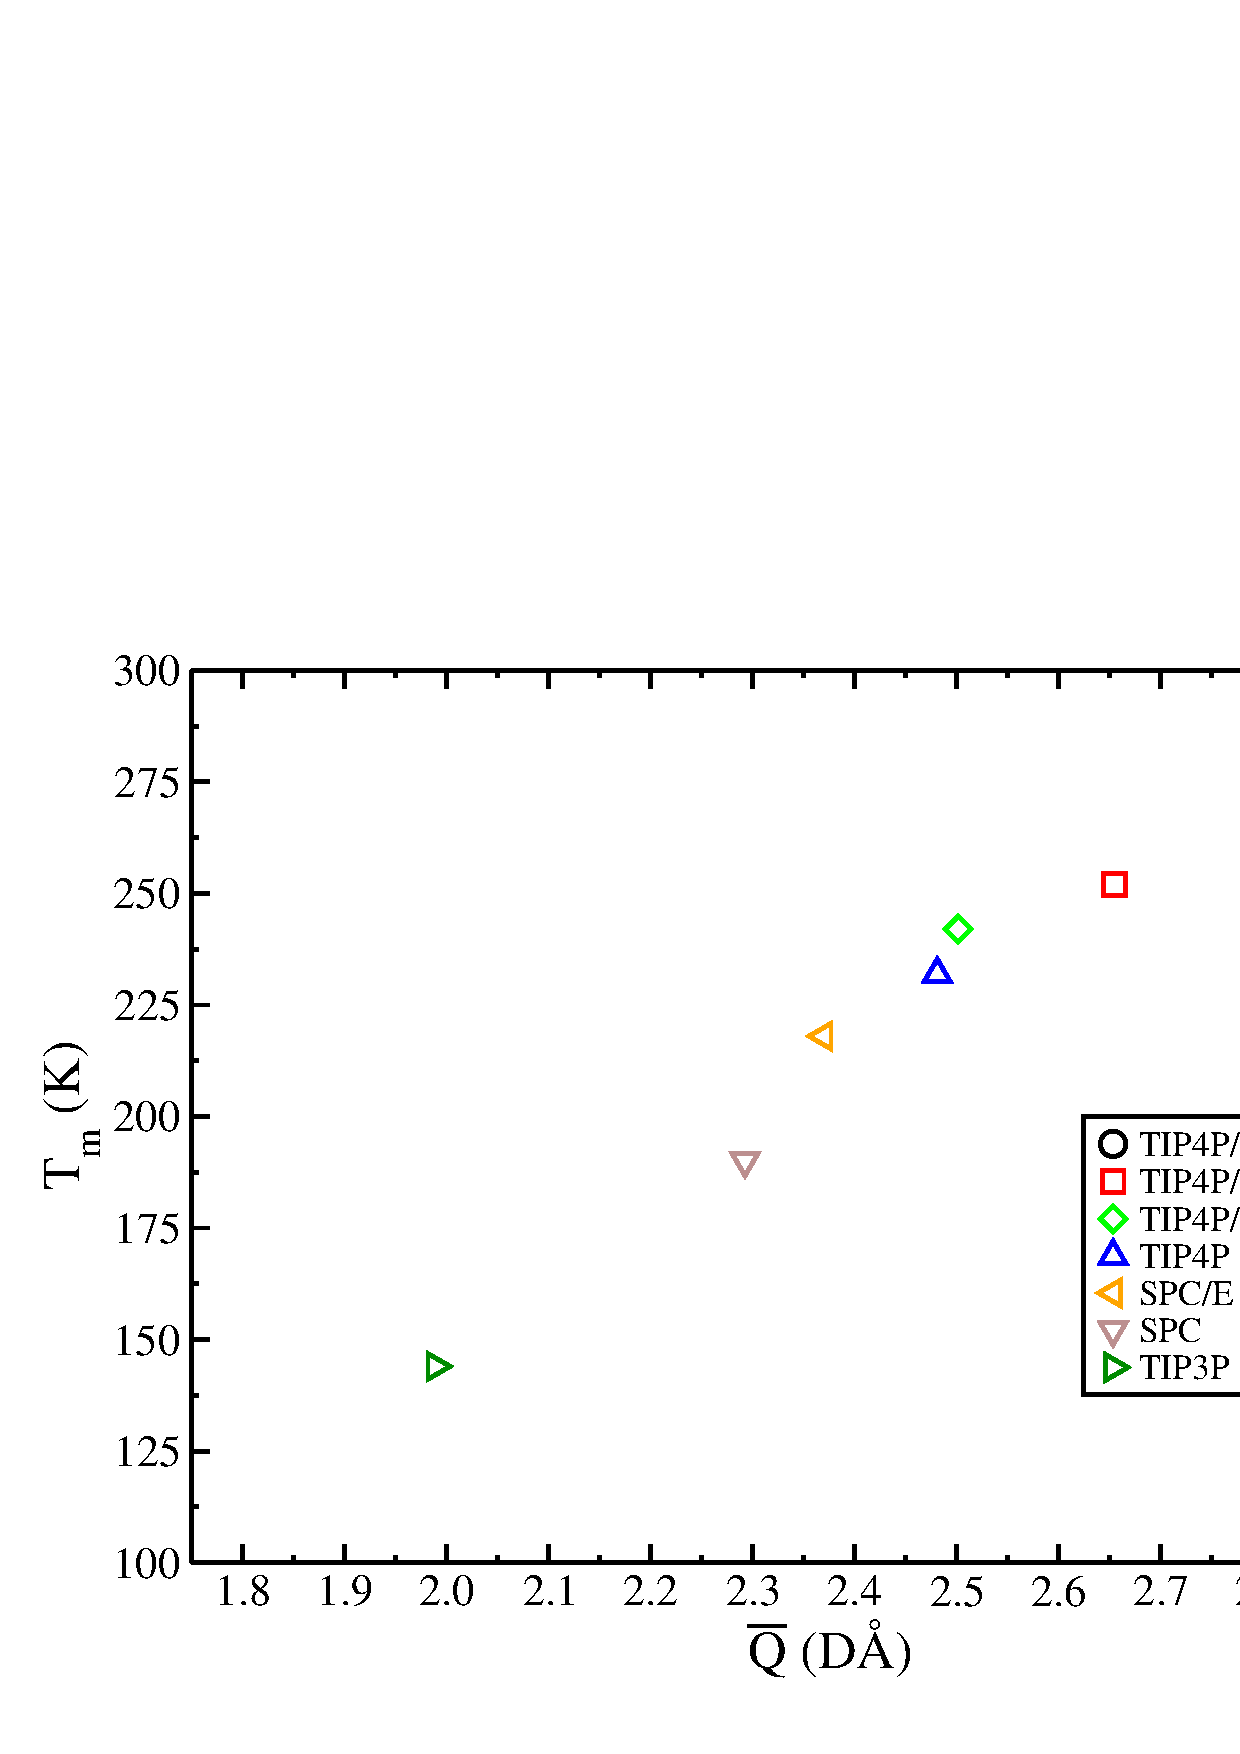
\includegraphics[width=\linewidth]{Figures/Tm_Ih_Qbar_plot.pdf}
\caption{\label{fig:QBar} Melting point for ice I$_h$ of several
  popular water models as a function of the QBar for the model. We see
  a strong correlation between a more accurate melting point and a
  larger value of $\overline{Q}$. We estimate that a $\overline{Q}$ of
  approximately 2.8 D\AA~will result in the experimental melting point
  of 273.15 K. A linear regression of the data resulted in an equation
  of best fit of $y = 158.89x - 166.83$. From this, we have predicted
  an optimal $\overline{Q}$ to be 2.7690 D\AA~.}
\end{figure*}

\begin{figure*}
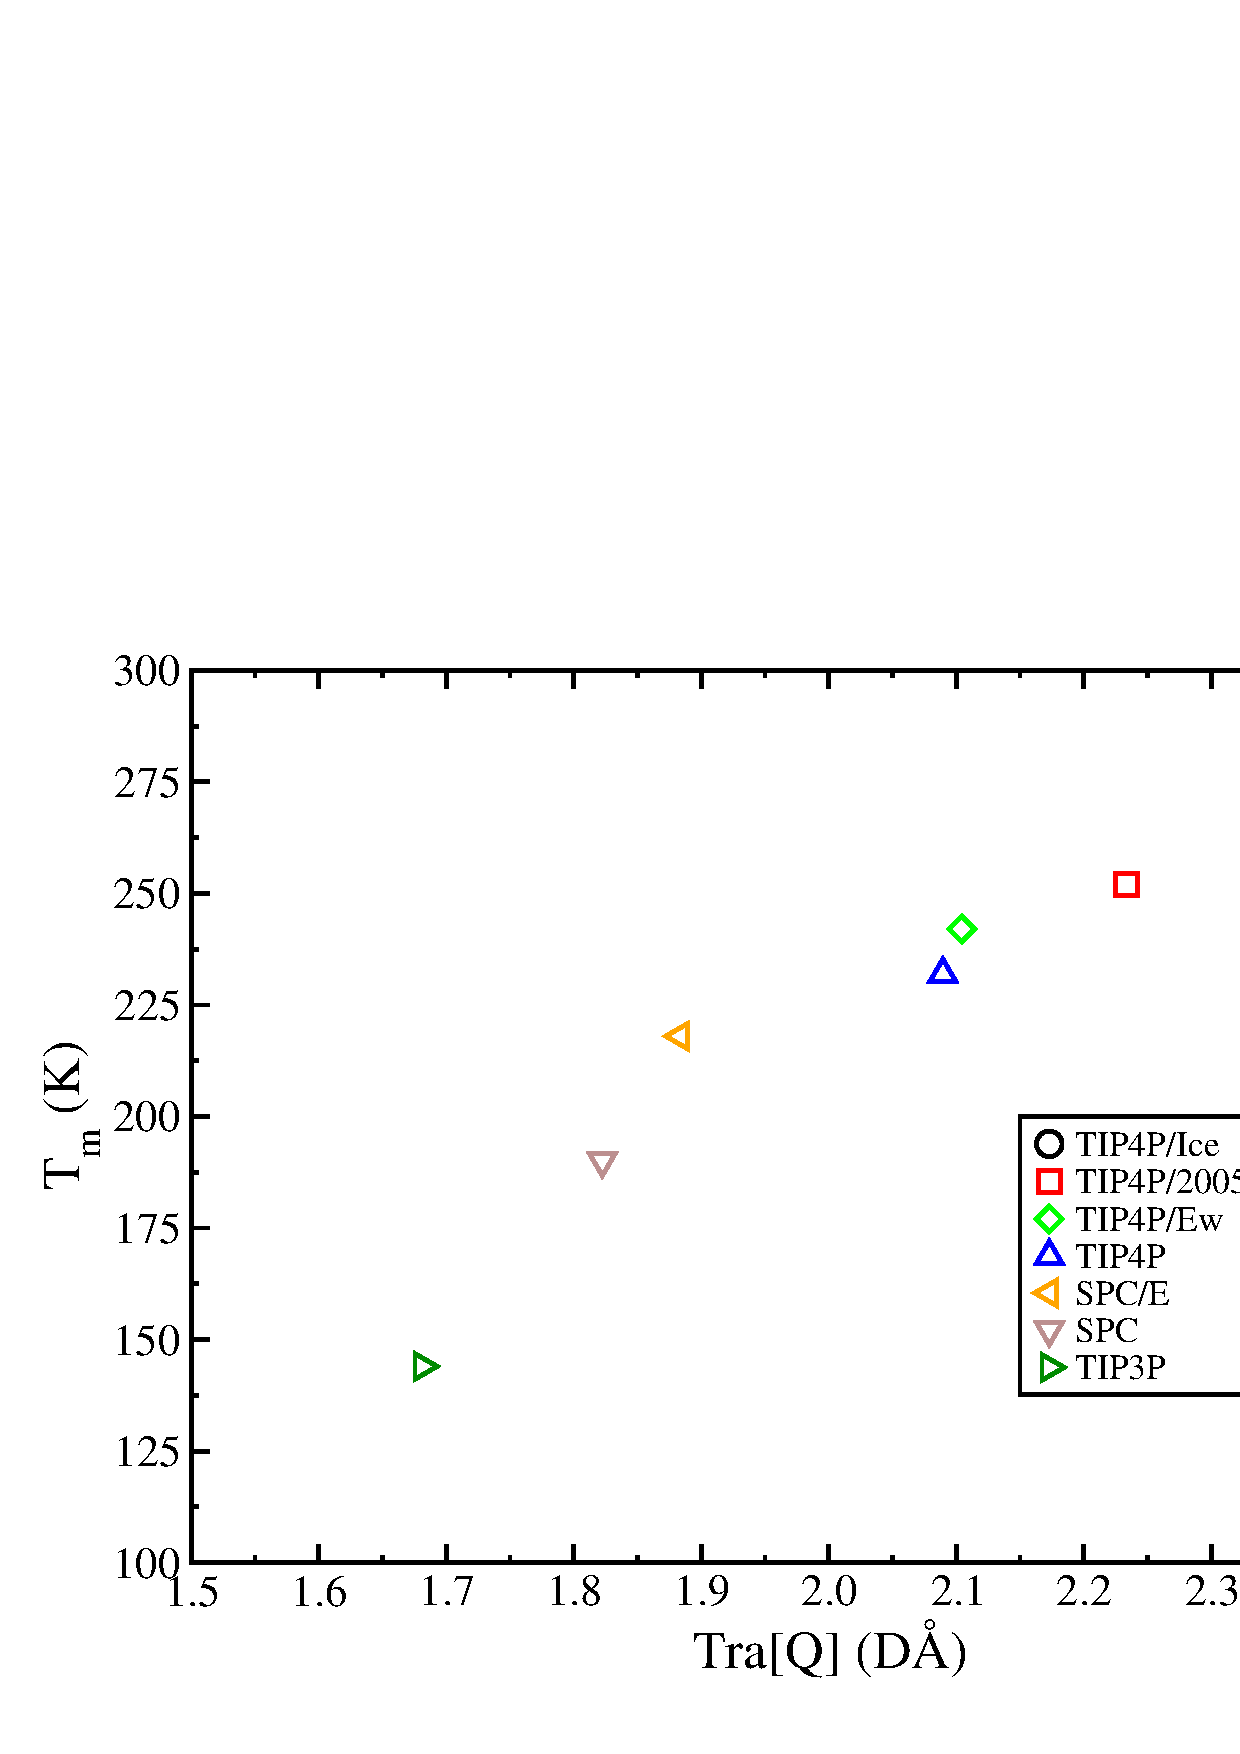
\includegraphics[width = \linewidth]{Figures/Tm_Ih_TraQ_plot.pdf}
\caption{\label{fig:TraQ} Melting point for ice I$_h$ of several popular water models as a function of the trace of the quadrupole tensor for the model. We see a strong correlation between a more accurate melting point and a larger value of the trace. We estimate that a trace of approximately 2.3 D\AA will result in the experimental melting point of 273.15 K.}
\end{figure*}

While it is still unclear if these results are indicative of an
experimentally observable phenomenon, exploring correlations such as
this can help in the development of water models in the future. 


\subsection{Transport Properties}
Transport phenomena are processes that describe the transfer (flux) of
mass, heat, momentum, and charge by molecular motions. During this
process, the transferred quantity is conserved, \textit{i.e.}, the
moving entity is neither created nor destroyed. Because of this, a set
of balance, or conservation equations can be written down describing
the movement of these quantities in the presence of a flux. The set of
balance equations for the transport of mass, energy and momentum are
presented in Table \ref{tab:transport}. 


\begin{table}
	\caption{BALANCE AND CONSTITUTIVE EQUATIONS FOR MASS, ENERGY, AND MOMENTUM TRANSPORT\label{tab:transport}}
        \begin{tabular}{rcc}
          \hline \hline
          & \textbf{~~Balance Equations~~} & \textbf{~~Constitutive Equations~~}\\ \hline 
          \textbf{~~Mass~~} & $\frac{\partial c (\vec{r}, t)}{\partial t} + \nabla \vec{j} = 0$ & $\vec{j} = -D \cdot \nabla c(\vec{r}, t)$\\
          \textbf{~~Energy~~} & $C_p \frac{\partial T (\vec{r}, t)}{\partial t} + \nabla \vec{J} = 0$ & $\vec{J} = -\lambda \cdot \nabla T(\vec{r}, t)$\\
          \textbf{~~Momentum~~} & $\rho \frac{D \vec{v}(\vec{r}, t)}{Dt}
                                  + \nabla \overleftrightarrow{\sigma} =
                                  0$ & $\sigma_{x,z} = -\eta \cdot
                                       \nabla_z (\rho v_x)$\\ \hline
          \hline
          \end{tabular}
\end{table}

When a transport flux is present, a characteristic response of the
material the flux is traveling through will become visible. For
example, in the presence of an energy flux, a thermal gradient will
develop in the material. Likewise, a momentum flux will cause a
velocity distribution to form in the system. Through a series of
constitutive equations, it is possible to relate the flux to the
observed system response through a proportionality constant describing
the transport. These constants are dependent on the material the
transport is occuring through, and thus are characteristic quantities
of the material. These constants have been well defined in both
homogeneous and heterogeneous systems, through bulk materials as well
as across interfaces.


\begin{itemize}
\item \textbf{Diffusion (Fick's Law):} $\vec{j} = -D \cdot \vec{\nabla}c(\vec{r},t)$ \vspace{0.05in}\\
The diffusion constant, $D$, relates the mass flux to the concentration gradient.
\item \textbf{Thermal Conductivity (Fourier's Law):} $\vec{q} = -\lambda \cdot \vec{\nabla} T(\vec{r},t)$ \vspace{0.05in}\\
The thermal conductivity, $\lambda$, relates the heat flux to the temperature gradient.
\item \textbf{Viscosity (Newton's Law of Viscosity):} $\sigma_{x,z} = -\eta \cdot \vec{\nabla}_z (\rho v_x)$ \vspace{0.05in}\\
The shear viscosity, $\eta$, relates the shear stress to the velocity gradient $\left < d(v_x)/dz \right >$.
\end{itemize}

\subsubsection{Green-Kubo Relations}
In the 1950s, Green and Kubo showed that transport coefficients
$\gamma$ are directly related to the time dependence of equilibrium
fluctuations in the associated flux $J$.
\begin{equation}\label{eq:greenKubo}
\gamma = \frac{V}{k_BT}\int_0^{\infy}ds\langle J(0)J(s)\rangle
\end{equation}
Here, $V$ is the volume of the system, $k_B$ is Boltzmann's constant,
and $T$ is the temperature.

\subsubsection{Non-equilibrium Molecular Dynamics Methods}
Due to the timescale of the simulations required, others have
approached the problem by performing non-equilibrium molecular
dynamics simulations. Here, the system is forced to be at some
non-equilibrium state, and the flux required to maintain that state is
calculated from the simulation. This process can be challenging,
however, simulation times are often shorter than those required for
using the Green-Kubo formalism. With the required flux in hand, the
transport property is calculated by using the relavent linear
constitutive relation. If the desired transport property is the
thermal conductivity ($\lambda$) of a material, two regions of the simulation box
will be thermostatted, and the kinetic energy flux ($J$) required to
maintain the temperature difference will be calculated. Once this
value is converged, $\lambda$ can be obtained by 
\begin{equation}\label{thermalTransport}
J_{z} = \lambda \big(\frac{\partial T}{\partial z}\big)
\end{equation}
where the separation has been taken to be along the $z$-dimension of
the system.  Here, $\big(\frac{\partial T}{\partial z}\big) $ is
determined by the temperature of the two regions and the distance the
regions are separated over. Similarly, the shear viscosity
($\eta$) of a fluid can be determined by forcing molecules at two
separated regions of the simulation box,
\begin{equation}\label{momentumTransport}
  j_{z}(p_{x}) = -\eta \big(\frac{\partial v_{x}}{\partial z}\big)
\end{equation}
where again the regions are taken to be separated along the
$z$-dimension of the simulation box.

In equilibrium molecular dynamics simulations, the transport
properties can be obtained by utilizing the Green-Kubo relations.
While it is possible to obtain the transport properties of interest
through equilibrium or non-equilibrium molecular dyamics simulations,
Kuang and Gezelter have recently developed an approach to
non-equilibrium molecular dynamics in which they invert the measured
and imposed quantites.


%%%%%%%%%%%%%%%%%%%%%%%%
% The grand intro, ancient greeks, life as we know it, etc.
%%%%%%%%%%%%%%%%%%%%%%%%
\section{H$_2$O: A Simple Molecule with Complex Behavior}
Water is the simplest compound of the two most common reactive
elements in the unvierse and it the second most common molecule in the
universe (behind hydrogen, H2). It is composed of two atoms of
hydrogen, and one atom of oxygen, and it has been found to be
fundamental to star formation.  Water is one of the most important
molecules found on our Earth.  It occurrs in natural abundance,
composing nearly XX percent of the molecules present. It is also one
of the few molecules that can be found in its solid, liquid, and
gasseous forms, occurring at ambient temperatures and pressures.  Some
hypothesize that life cannot exist without water, as we have not found
a case of life without it. In many organisms, water comprises XX
percent of their chemical makeup, with as large as XX in others. In
humans, water composes XX percent of our bodies. It is the ubiquitus
nature of water and ice that gives rise to its importance; due to its
natural abundance a wide variety of chemistry and physical processes
occur within this medium, and at its surfaces.

In ancient times, humans recognized the importance of water. The Greek
philosopher Thales of Miletus, one of the seven sages of antiquity
declared that everything was composed of water (around 700 BCE). Later
on in the 5th century BCE, Empedocles described water as being one of
four 'classical' elements of the ancient world, earth, wind, fire, and
water. Even the ancient Chinese described the world around them using
five elements, earth, wood, metal, fire, and water. The importance of
water was discovered early in our human history, and it has been
studied extensively since those early days.  

%How water's properties are encoded in its molecular structure and
%energies. Chemical Reviews. Brini et al. 2017.
It has volumetric anomalies-water’s solid (ice) floats on its liquid;
pressure can melt the solid rather than freezing the liquid; heating
can shrink the liquid. It has more solid phases than other materials.

Water is highly abundant on Earth, occupying
$1.4x10^{9} km^{3}$.\cite{2-4} It is the most abundant greenhouse gas
in the atmosphere, accounting for 40 percent to 70 percent of Earth's
retention of heat.

All forms of life depend on water.\cite{5,6} Approximately half of the
volume of every cell is water.\cite{7} Water plays a rich role in
biochemical processes, where it has been seen to act as a solvent,
reactant, product, catalyst, chaperone, messenger, and
controller. Water also plays a dominant role in the complex folding of
proteins.

Our species is highly dependent on the solubility of gasses in liquid
water. Beyond the movement of oxygen (O$_{2}$) throughout
our bodies, much of the oxygen we breathe is produced by sea
life. These marine plants require carbon dioxide
(CO$_{2}$) in order for photosynthesis to produce
carbohydrates and release oxygen. However, the solubility of gasses in
water is highly sensative to temperature, pressure, and salinity. 

Water molecules associate with each other relatively
tightly. Therefore, H2O has relatively high values of surface tension,
melting point, and boiling point.

water has a relatively high surface tension, of 72.8 mN m−1 at room
temperature, due to its high cohesion, the highest of the common
nonionic, nonmetallic liquids.
% end Chemical Reviews. Brini et al. 2017.

% John Finney, A Very Short Introduction to Water. Oxford University
% Press. 
In normal ice, water molecules form puckered six member rings, with
OOO angles formed by three neighboring molecules close to 109.5
degrees. Perhaps include an image of ice with just the oxygen sites
shown? Looking at the figure of ice, we see that it is fairly
open. What we mean by this, is that we can see through the structure,
from one side to the other. If we compare this to that of a liquid, in
the lower panel of the same image, we see that we are unable to see
through to the other side of the simulation cell. This is indicitive
of the differences in density between the solid and liquid phases of
water, namely, that the solid phase has a smaller density than the
liquid. Looking at the solid phase in the figure, one may wonder if
subsequent water molecules would fit within the open channels of the
ice. Indeed molecules can be found in these channels, however, they
are unable to form hydrogen bonds with water molecules constituting
the ice lattice. Molecules of this nature are only observed in
ultra-high density ices, ice-number and ice-number, for example. In
these crystal structures, two ice lattices are inter-twined within one
another. That is, a secondary ice lattice is present interwoven
through the first, where no cross hydrogen bonding between the two
lattices exist.

Maybe describe a few of the phase transitions of ice Ih? Ice Ih at -30
degrees Celcius, apply 30,000 atmospheres of pressure and we will
observe a phase transition to ice-III. Similarly, cool ice-III to -40
degrees Celcius and we will see a phase transition to ice-II. There
are approximately sixteen different known crystal structures of ice,
each one stable in some unique region of the phase diagram. Also,
there are ice phases which have been predicted by computer simulation
which have not yet been observed in vivo. If we inspect the phase
transition from ice Ih to ice-III closer, we will see a distortion in
the crystalline geometry under the large pressure conditions. Some of
the puckered six-membered rings will compress into five-membered
structures, resulting in a more dense packing of water
molecules. However, this will place more strain on the
hydrogen-bonds. In ice-III, the OOO bond angles vary between 88
degrees and 148 degrees. Likewise, the hydrogen-bond lengths will also
change under this distortion. In ice-Ih, hydrogen-bonds are typically
0.276 nm, in ice-III hydrogen-bonds are found between 0.271 nm and
0.283 nm.

ice XVI, discovered in 2014, is metastable under ambient and high
pressure, but is postulated to be stable under negative pressure,
\textit{i.e.} under lattice tension. Therefore, the region of
stability might be to the left of that shown in the phase diagram,
beyond the $P = 0$ vertical. Image of water molecules (maybe 5 of
them) where the hydrogens are permuted through the possible
combinations. From this figure, we see that several possible
combinations of hydrogen arrangements are possible. These are all
equivalent, and they follow the original set of rules laid down by
Bernal and Fowler in 1933. These rules are as follows,
One. Each oxygen atom is covalently bonded to two hydrogens. This is
essentially the definition of being a water molecules. Two. Each
hydrogen in each water molecule forms a hydrogen bond with one other
oxygen, therefore, there is exactly one hydrogen between every two
oxygen sites in the lattice. The result of these rules is that each
oxygen is in a tetrahedral environment, and is donating two hydrogens
and accepting two hydrogen bonds. 

If we now consider how we might populate the hydrogens into the oxygen
lattice while obeying these ice-rules, we see there are two
\textit{kinds} of crystals that can be obtained, \textit{ordered} and
\textit{disordered}. In the \textit{ordered} case, the orientations of
equivalent water molecules in all unit cells are the same, whereas in
a \textit{disordered} ice the orientations of equivalent water
molecules are not the same. This can be seen in figure (insert figure
showing proton ordered vs disordered here). While we can speak of
these lattices as water molecules that are orientationally ordered or
disordered, often this is described in terms of proton order and
disordered cases. The two descriptions are equivalent as the
arrangement or ordering of the hydrogens gives rise to the orientation
of the water molecules. ices Ih, III, IV, V, VI, VII, XII, XVI are
orientationally disordered, while ices II, VIII, IX, and XI are
orientationally ordered. Upon cooling, ice III and ice VII (disordered
ices) will undergo a phase transition to ordered forms, ice IX and ice
VIII respectively. Transitions of proton disordered ice to proton
ordered ice must inherently involve the reorientation of water
molecules, or the transfer of hydrogens, or some combination of the
two. However, if all molecules in the lattice satisfy the Bernal
Fowler ice rules, any one water molecule reorientation or proton
transfer will inevidebly break the ice-rules. Therefore, we conclude
these events must happen in concert, large collections of molecules
must simultaneously undergo some combination or reorientation and
proton transfer. However, the energy required to do so would be quite
large, and larger still for increasing number of molecules
involved. This amount of energy is not likely available at the thermal
conditions where these transitions are observed to occur, thus it is
believed that the these transitions must depend on defects within the
lattice. There are two known kinds of defects in ice
lattices. \textit{Orientational} defects, known as Bjerrum defects after the
person who proposed the idea, and \textit{ionic} defects. First, there
are two kinds of Bjerrum defects, D-defect (from the German
\textit{doppelbesetze} meaning doubly occupied), and an L-defect (from
\textit{leere} meaning empty). From the figure, we see that a D-defect
occurs when there are two hydrogens between two oxygen sites, and an
L-defect occurs when there are no hydrogens between two oxygen
sites. These are of course in violation of the Bernal Fowler
ice-rules, however, they act as proton sinks and sources when the
crystal undergoes phase transitions from proton disordered to proton
ordered. The presence of these sites lowers the energy required, and
maybe I can find a citation about this. Ionic defects occur when a
proton transfer happens and the resulting lattice has a hydroxide and
hydronium ion.



%end A Very Short Introduction to Water.

\subsection{The Structure of H$_\mathrm{2}$O}
%
% description of what water is? structure constitution etc?
% Gas phase molecule in isolation
% Condensed phase liquid water as collection
% Description of ice and it's structures
%
Defining water's structure can prove a bit challenging. In isolation
in the gas phase, water adopts a 'bent' like geometry, with an HOH
bond angle of about 104.5 degrees. The oxygen-hydrogen bond length as
computed by high accuracy quantum mechanical calculations gives 1
\AA~. These bond lengths and bend angles are an equilibrium value, as
they are constantly vibrating. Even at $-$273.15 degrees Celcius (0
Kelvin) some residual vibrations remain. This is described as a
zero-point energy, and has considerable implications for the potential
energy of the molecules. 

Water's electrons are not distributed about the molecule
symmetrically. This gives rise to higher order multipoles, and it is
these electronic characteristic that give rise to many of water's
characteristic properties. In the gas phase, water has a dipole moment
of about 1.85D. This dipole moment is highly polarizable, that is, it
responds to an external electric field, be it an applied one or the
field created by molecules in its local environment. In the presence
of an external field, the valence electrons in water respond by
separating even more, resulting in a larger dipole moment for the
molecule. In the condensed liquid phase, this value becomes much
harder to probe experimentally, but values have been reported ranging
from 2.2D to 2.9D. 

High accuracy QM calculations on collections of water molecules?


This dissertation is a study of water, often in coexistence between
two of its many phases. The current phase diagram for water is shown
in figure \ref{fig:phaseDiagram}.

\begin{figure}
\includegraphics[width=\linewidth]{Figures/PhaseDiagram}
\caption{\label{fig:phaseDiagram} The phase diagram of
  water.\cite{Zhang2015} dT$_{C}$ / dP $<$ 0 at the following boundaries:
  ice-II to ice-V, liquid to ice-I$_\mathrm{h}$, and ice-VII to
  ice-VIII. Conversely, dT$_{C}$ / dP $>$ 0 at the following boundaries:
  liquid to vapour, liquid to ice-(V, VI, VII). dT$_{C}$ / dP $\approx$
  $\inf$ at the ice-(VII, VIII) to ice-X boundary occurring at 60 GPa.
  dT$_{C}$ / dP $\approx$ 0 at ice-I$_\mathrm{h}$ to ice-XI boundary at
  low temperatures. }
\end{figure}


\begin{table}[h]
\centering
\caption{Physical Properties of the Various Ice Forms }
\label{tab:iceProps}
\begin{tabular}{|cccc|}  \hline 
  ice form & crystal structure & density (g cm$^{-3}$) & proton arrangement  \\ \hline
  I$_\mathrm{h}$ & hexagonal & 0.92 & disordered \\
  I$_\mathrm{c}$ & cubic & 0.93 & disordered \\
  II & rhombohedral & 1.17 & ordered \\
  III & tetragonal & 1.14 & disordered \\
  IV & rhombohedral & 1.27 & disordered \\
  V & monoclinic & 1.23 & disordered \\
  VI & tetragonal & 1.31 & disordered \\
  VII & cubic & 1.50 & disordered \\
  VIII & tetragonal & 1.46 & ordered \\
  IX & tetragonal & 1.16 & ordered \\
  X & cubic & 2.51 & symmetric \\
  XI & orthorhombic & 0.92 & ordered \\
  XII & tetragonal & 1.29 & disordered \\
  XIII & monoclinic & 1.23 & ordered \\
  XIV & orthorhombic & 1.29 & ordered \\
  XV & pseudoorthorhombic & 1.30 & ordered \\
  XVI & cubic & 0.81 & disordered \\ \hline
\end{tabular}
\end{table}

\subsubsection{Liquid Water}
It is this dipole moment polarization in conjunction with hydrogen
bonding which gives rise to water being a liquid at room
temperatures. The strength of the hydrogen bond between two water
molecules is somewhere between the strong covalent bonding
interactions holding the individual water molecules together, and the
weaker van der Waals interaction due to the instantaneous polarization
of molecules electronic clouds of electrons. Numerically, hydrogen
bonds have a strength of about 20 J/mol, about ten times thermal
fluctuation at room temperature. This ratio is important in the
cohesion of molecules into a condensed phase. For water, the order of
magnitude difference between the intermolecular interactions and
thermal fluctuations means that the liquid will not boil at room
temperatures. Intermolecular forces for many other smaller molecules
are not as strong as the hydrogen bonding observed in water. The
intermolecular interactions of H2S are much weaker, for example, and
it boils at -60 degrees Celcius. Most other molecules that weigh on
the order of 18 amu are gasseous at room temperature. The strong
dipole moment of water holds the molecules together in a condensed
phase.

Another interesting property of the hydrogen bond is its
directionality and number of neighbors that bond with it. The proton,
electron distribution, and higher multipole moments that give rise to
the strength of the hydrogen bonds also give rise to the local
structure of liquid water. Water molecules hydrogen bond to a central
molecule forming a tetrahedral configuration. In liquid water,
molecules form local tetrahedral environments Liquid water transitions
to ice when the local ordering becomes long ranged.


\subsubsection{Water Ice}
%
% Describe crystal structures of ice, examples of where some occur.
% Proton disordered structure, residule entropy. 
%
%Annu. Rev. Phys. Chem. 2017. 68:285–304
'Ice is a fundamental solid with important environmental, biological,
geological, and extraterrestial impact.'\cite{Shultz2017} 'Ice is
arguablyamongthemostfundamental andubiquitous solids in the Universe
(1–3).Consisting of two of the threemost abundant elements, ice and
its liquid form, water, not only shapeEarth and our Solar System but
also transportmaterial throughout the Universe.' 

'Ice is challenging in part due to configurational flexibility
exemplified by the famous residual entropy of ice at 0K(4).The source
of residual entropy lies in the tetrahedral coordination around the
oxygen atom: Two coordinations are bonds to hydrogen atoms and two are
lone pairs. Hence, water forms an extended network, but there is
considerable flexibility for locating the hydrogen atoms to satisfy
the “ice rules” (5): exactly one hydrogen atommust be located between
any pair of oxygen atoms and every oxygen atom must be covalently
bonded to exactly two hydrogen atoms. Surface termination leads to
dangling valences. Dangling valences, even at the ideal surface, can
be random or patterned (6–10). Finally, as is common with many solids,
the ice surface can relax and/or reconstruct.'

(on qll) 'techniques as diverse as glancing angle X-ray (102, 103),
SFG (82), He atom scattering (104), atomic force microscopy (105,
106), ellipsometry (107), photoelectron spectroscopy (108), nuclear
magnetic resonance (NMR) (109, 110), theory (111–114), and
differential interference contrast (57, 115, 116) conclude that the
QLL exists.' The onset temperature has varied from as cold as 200K to
as warm as 260K, and discrepencies have been attributed to
contaminations to varying probe depths. There is also considerable
disagreement about the nature of the QLL, 'Theory indicates that it is
ordinary supercooled water (117), whereas recent interfacial force
microscopy (105) suggests that the QLL is neither ice nor water but
rather a new viscoelastic phase.' And recently Suzuki \textit{et al.}
have probed the QLL and observed two separate immesible liquid water
flims. 

Section 4.1 deserves further reading, talks about thermodynamics of
the basal, prism, and secondary prismatic crystal surfaces.
%end Annu. Rev. Phys. Chem. 2017. 68:285–304

Water crystallizes into ice in a wide variety of different spacial
arrangements. There are currently 16 known crystal structures of ice,
some of which only occur at large pressure environments and are
thought to be present on the moons of SaturnXX, while others have yet
to be observed but are predicted by computer simulations. Here on
Earth, the most common form of ice is ice-I$_\mathrm{h}$, which has 6
molecules in the unit cell and crystallizes under the P6mm3 space
group.

The structure of ice-I$_\mathrm{h}$ has been studied extensively using
experimental methods such as neutron scattering and x-ray
spectroscopy, as well as NMR and laser spectroscopy.\cite{w. F. Kuhs
  and M. S. Lehmann, in Water Science Reviews 2, edited by F. Franks
  (Cambridge University, New York, 1986),pp. 1-65.} 

From these, a set of 'ice-rules' have been established by Bernal and
Fowler.\cite{XX} These rules describe the required metrics for accurate
crystals of ice-I$_\mathrm{h}$. Residual entropy due to hydrogen
disordering. Hayward and RameiresSP developed an algorithm for
sampling of ice-I$_\mathrm{h}$ crystals.\cite{HaywardXX}

\subsubsection{Residual Entropy of Ice}
If we further consider the Bernal-Fowler ice rules, we see that the
hydrogen arrangement in ice I$_\mathrm{h}$ is not unique. In 1935,
Linus Pauling argued that any arrangements of hydrogens which
satisfies the ice rules is valid and has equal probability of
occuring since each unique arrangement has the same energy,
\textit{i.e.} they are degenerate configurations. Due to this, he
predicted ice I$_\mathrm{h}$ to have a \textit{residual entropy}, that is, a
non-vanishing positive entropy ($S_{0}$) at zero Kelvin. This entropy
can be computed from Boltmann's equation of statistical mechanics,
\begin{equation}\label{Boltzmann-W}
S = k_{B}~ln(W)
\end{equation}
where $k_{B}$ is Boltzmann's constant and $W$ is the number of
equivalent arrangements of the molecules. Pauling estimated the number
of configurations in two separate ways.\cite{Pauling1935} First, we
consider that there are possible six ways to orient a water molecule
within a tetrahedral structure formed by neighboring molecules while
satisfying ice rule number NUM. If we give each water molecule one of
these six orientations at random, there is then a 1/2 probability of
having a hydrogen between two oxygens, thus there is a 1/4 chance of
satisfying ice rule NUM, that there is exactly one hydrogen between
every two oxygens in the lattice. The resulting number of correct
possible arrangements of $N$ water molecules is
\begin{equation} \label{Pauling-1}
W_{Pauling} = (6/4)^{N} = (3/2)^{N}.
\end{equation}   
Pauling arrived at the same result by a second construction. If we
ignore ice rule NUM, and only enforce there to be a single Hydrogen
between each Oxygen in the lattice, there are $2^{2N}$ configurations
(since there are $2N$ bonds in the network). For each Oxygen atom,
here are $2^{4} = 16$ possible arrangements for the Hydrogens, 10 of
which are ruled out by ice rule NUM, as they result in non-intact
molecules. That is, they form structures of (H$_{4}$O)$^{2+}$,
(H$_{3}$O)$^{+}$, (HO)$^{-}$, and O$^{2-}$. Therefore, there are only
6/16 possible configurations allowed for placing Hydrogens around each
Oxygen. This gives a total number of configurations as,
\begin{equation}
W_{Pauling} = 2^{2N}(6/16)^{N} = (3/2)^{N}.
\end{equation}
Using these results with equation \ref{eq:Boltzmann-W}, the residual
entropy follows as
\begin{equation}
S_{0} = k_{B}Nln(3/2) = Rln(3/2)
\end{equation}
where $R$ is the molar gas constant, $R = 8.31447 J
mol^{-1}K^{-1}$. This gives a residual entropy of 
\begin{equation}
S_{0} = 3.3712 J mol^{-1}K^{-1} = 0.80574 cal deg^{-1} mol^{-1}.
\end{equation}
The residual entropy has been further investigated by Berg \textit{et
  al.} who obtained $S_{0} \approx 0.81550 \pm 0.00021 cal deg^{-1}
mol^{-1}$ by means of multicanonical simulations.\cite{Berg2007} This
result was found to be in good agreement with a series expansion
method by Nagle \textit{et al.}\cite{Nagle1966}, as well as Giaque and
Stouts calorimetry experiments which estimated $S_{0} = 0.82 \pm 0.05
cal deg^{-1} mol^{-1}$.\cite{Giaque1936} 

\subsection{Ice/Water Coexistence}
%%%
% General introduction to ice/water coexistence
% Early work in the field, quiescent systems and measures of
% interfacial width.
% Problems discovered specific to ice/water coexistence, improper
% treatment of the electrostatics, coexistence temperatures, etc.
%
%%%


%%%
% from iceWater.tex
%
%
%%%

Understanding the ice/water interface is essential for explaining
complex processes such as nucleation and crystal
growth,\cite{Han1992,Granasy1995,Vanfleet1995} crystal
melting,\cite{Weber1983,Han1992,Sakai1996,Sakai1996B} and some fascinating
biological processes, such as the behavior of the antifreeze proteins
found in winter flounder,\cite{Chapsky1997 ,Wierzbicki2007} and certain
terrestrial arthropods.\cite{Duman:2001qy,Meister29012013} There has
been significant progress on understanding the structure and dynamics
of quiescent ice/water interfaces utilizing both theory and
experiment.  Haymet \emph{et al.} have done extensive work on ice I$_\mathrm{h}$,
including characterizing and determining the width of the ice/water
interface for the SPC,\cite{Karim1990} SPC/E,\cite{Gay2002,Bryk2002} CF1,\cite{Hayward2001,Hayward2002} and TIP4P~\cite{Karim1988} models for
water.
More recently, Haymet \emph{et al.} have investigated the effects
cations and anions have on crystal
nucleation.\cite{Bryk2004,Smith2005,Wilson2008,Wilson2010} Nada \emph{et al.}
have also studied ice/water
interfaces,\cite{Nada1995,Nada2000,Nada2003,Nada2012} and have found that the
differential growth rates of the facets of ice I$_\mathrm{h}$ are due to the the
reordering of the hydrogen bonding network.\cite{Nada2005}

The movement of liquid water over the facets of ice has been less
thoroughly studied than the quiescent surfaces. This process is
potentially important in understanding transport of large blocks of
ice in water (which has important implications in the earth sciences),
as well as the relative motion of crystal-crystal interfaces that have
been separated by nanometer-scale fluid domains.  In addition to
understanding both the structure and thickness of the interfacial
regions, it is important to understand the molecular origin of
friction, drag, and other changes in dynamical properties of the
liquid in the regions close to the surface that are altered by the
presence of a shearing of the bulk fluid relative to the solid phase.

In this work, we apply a recently-developed velocity shearing and
scaling approach to reverse non-equilibrium molecular dynamics
(VSS-RNEMD). This method makes it possible to calculate transport
properties like the interfacial thermal conductance across
heterogeneous interfaces,\cite{Kuang2012} and can create simultaneous
temperature and velocity gradients and allow the measurement of
friction and thermal transport properties at interfaces.  This has
allowed us to investigate the width of the ice/water interface as the
ice is sheared through the liquid, while simultaneously imposing a
weak thermal gradient to prevent frictional heating of the interface.
In the sections that follow, we discuss the methodology for creating
and simulating ice/water interfaces under shear and provide results
from both structural and dynamical correlation functions.  We also
show that the solid-liquid interfacial friction coefficient depends
sensitively on the details of the surface morphology.


% General intro to ice/water coexistence
Understanding the ice/water interface and the properties of the
molecules at the interface is important for many areas, including the
process of nucleation and crystal growth or melt. Biologically,
understanding this interface is vital for progression towards
understanding how antifreeze proteins work. Talk about some popular
antifreeze proteins, which have been shown to disrupt the hydrogen
bonding network at the interface. Some have been found to dock on the
ice surface / interface. A clearer picture of the structure and
dynamics of the molecules at the ice/water interface can help us
understand how antifreeze proteins work.

% Omar A. Karim and A.D.J. Haymet ChemPhysLett, 138, 6, (1987) 531
In one of the first computer simulations of the ice/water interface,
Karim and Haymet investigated the basal face of an ice-I$_\mathrm{h}$
crystal solvated in bulk water using the TIP4P model of water, where
they observed ice/water coexistence at 240$\pm$5~K. Calculating the
distance across which the oxygen-site density decays from the
twin-peaked ice structures to that of bulk liquid, they estimated the
basal ice/water interface to be approximately 10 \AA~ to 15 \AA~
wide. They further partitioned the system into 3.7 \AA~ wide bins, and
calculated the average self diffusion constant for molecules in each
bin. As the interface was traversed, the diffusion constant decays
from the bulk liquid value to approximately zero.
% End  ChemPhysLett, 138, 6, (1987) 531

% Omar A. Karim and A.D.J. Haymet J.Chem.Phys 89, 11 (1988) 6889
TIP4P basal ice/water interface, larger than previous study. They
compute g(r) for the bulk liquid and show it agrees with recent
neutron scattering data.  While investigating the orientational
structure of the interface, they found that the orientational order
induced by the ice crystal propogates at least one, and possible two
layers deeper into the water than the translational order (ie the
density defined by the oxygen positions). Orientational ordering of
the liquid which from density profiles looks like liquid water, but
orientationally still exhibits perturbations due to the
interface. They observed the same interfacial width using a larger
system (and the same metric of measure, the density of oxygen sites).
% End  J.Chem.Phys 89, 11 (1988) 6889

% T. Bryk and A.D.J.Haymet J. Chem. Phys. 117 (2002) 10258
% make sure I have all of haymets papers.
The basal and prismatic facets of ice Ih using SPC/E water in
temperature range of 220 - 240 K and 1 atm. Density, translational,
orientational, and dynamic order parameters indicate a smooth change
from ice to bulk liquid, indicative of a diffuse interface. The
interfaces are observed to be stable at 225 $\pm$ 5K (though this is
later revisted and shown to be 215K by Vega and others). 

Kusalik \textit{et al.} simulated ice nucleation using the SPC/E model
in the presence of a large external electric field.\cite{14} Baez and
Clancy investigated the ice/water interface using non-equilibrium
molecular dynamics.\cite{15} Without careful treatment of the
long-range electrostatic portion of the potential energy, sparious ice
motifs have been found to form, including a quartzlike proton-ordered
structure not (yet) found in real systems.\cite{16} 

citations 22 through 24 are about antifreeze proteins, steal them for
broader intro to ice/water coexistence. 

Bryk and Haymet set out to properly treat the long-range Coulomb
interactions with Ewald summation method, whereas Baez and Clancy
(also studying basal and prism ice/water interfaces using SPC/E,
however, switching function at 6 \AA~ which went to zero at 9 \AA~ for
speed of computation.) 

Ice crystal construction constrained to have zero net dipole and some
higher order multipoles, using the method employed by Hayward in the
CF1 paper. I'm betting it's the Hayward and Reimers construction. 

Bryk uses the original parameters of Berendesn's SPC/E model, not the
updated one?
%end Bryk and A.D.J.Haymet J. Chem. Phys. 117 (2002) 10258

% Benet, MacDowell, Sanz, PCCP 2014, 16, 22159
% A study of the ice/water interface using the TIP4P/2005 water model
Benet \textit{et al.} have measured the interfacial free energy of ice
Ih in coexistence with liquid water at 248.5~K by using the TIP4P/2005
water model by analysing the spectrum of capillary fluctuations at the
interface.\cite{Benet2014} This method was originally described by
Hoyt \textit{et al.}\cite{Hoyt2001}, has been used to calculate the
interfacial free energy of hard spheres,\cite{14} the Lennard-Jones
potential,\cite{15} and dipolar fluids.\cite{16}

In this method, water molecules were labeled as ice-like or
liquid-like based on local bond order parameters. Next, a discretized
profile parrallel to the interface (i.e, along the $x$ dimension),
$h(x_{n})$, was computed for many small bins across the system. These
resulting profiles were then Fourier-transformed,
\begin{equation}
h_{q} = \frac{1}{N}\sum_{n=1}^{N} h(x_{n})e^{iqx_n}
\end{equation}
giving an amplitude $h_{q}$ for each wave vector $q$, for each of the
$N$ total bins across the $x$-dimension. 

Capillary wave theory provides a relationship between these wave
vector amplitudes and the interfacial stiffness, $\sigma$ by
\begin{equation}
\langle |h_{q}|^{2} \rangle = \frac{k_{B}T}{A \sigma q^{2}}
\end{equation}
where $A$ is taken to be the product of the two simulation box
dimensions not normal to the interface. Since the interfacial
stiffness is dependent on both the crystal plane that is exposed to
the liquid and the direction which the wave vector propogates, we have
\begin{equation}
\sigma = \bigg(\gamma (\theta ) + \frac{d^{2}\gamma (\theta )}{d\theta
^{2}} \bigg)_{\theta = 0} .
\end{equation}
Here, $\theta$ is the angle between the average planar ice / water
interface, and the normal vector of the instantaneous interface. The
orientational dependence of the interfacial free energy can be written
as an expansion of the Spherical Harmonics\cite{23}, and will be
unique for each crystal plane studied. 

Benet found an orientationally averaged interfacial free energy of
$27 \mathrm{mN} \mathrm{m}^{-1}$, which agrees well with recent
estimates using size cluster analysis by Sanz \textit{et
  al.}\cite{Sanz2013}. Benet \textit{et al.} were able to estimate the
free energy of different planes (in coexistence with liquid), and
obtained values of 27 $\pm$ 2, 28 $\pm$ 2, and 28 $\pm$ 2
$\mathrm{mN} \mathrm{m}^{-1}$ for the basal, prismatic, and secondary
prismatic surfaces, respectively. They also observed an interfacial
thickness of about four to five molecular diameters, which was found
to be (in)sensitive to the crystal face exposed to the liquid. Lastly,
when the basal face is exposed to the liquid, they observed local
areas of hexagonal ice and cubic ice within the interface. This
observation is not unique to this study, other simulations and
experiments have shown hexgonal ice to grow with a mixed Ic-Ih
stacking.\cite{43-47}

The interfacial free energy between ice and water, $\gamma_{iw}$, is a
crucial parameter for ice nucleation and crystal growth.\cite{1,2}
Experimentally obtained values of $\gamma_{iw}$ range from 25 to 35
$\mathrm{mN} \mathrm{m}^{-1}$.\cite{1} This spread stems from the
problem that there are no current methods for obtaining a robust
measurement. Computer simulations have attempted to quantify
$\gamma_{iw}$, and predictions have been made for a series of water
models, some with\cite{4} and some without\cite{5} taking full
electrostatic interactions into account. These studies used a varient
of the cleaving method,\cite{6} and estimated $\gamma_{iw}$ using the
TIP4P, TIP4P-Ew, and TIP5P-E water models.

Previously, $\gamma_{iw}$ has been estimated using the TIP4P/2005
water model and the method pruposed by Bai and Li, studying the
crystal-melt interface of a Lennard-Jones system.\cite{10} In the
method of Bai and Li, the critical size of crystalline clusters are
measured, and by extension of classical nucleation theory
$\gamma_{iw}$ can be obtained.\cite{11,12} This result produces an
orientationally averaged estimate of $\gamma_{iw}$, which does not
provide any information on the dependency of $\gamma_{iw}$ on the
orienation of the crystal.



%end Benet, MacDowell, Sanz, PCCP 2014, 16, 22159





\subsection{The Surface Premelting of Ice and the Quasi-Liquid Layer}
% 1. Surface cuts of ice-Ih, what do they look like, energetics of
% each. Have image of each surface here, talk about physical structures
% of each, dimensions of channels. Proton ordered surfaces vs proton
% disordered surfaces.
% 2. Driving force for the QLL, not unique to ice. Interesting on ice
% because ice occurs everywhere in the universe, therefore, lots of
% interesting things happen at ice surfaces.
% 3. Experimental and theoretical measures of the QLL, who and how have
% studied it.
% 3a. QLL width
% 3b. QLL structure, dynamics
% 4. Observed oddity of friction on ice surfaces is small, transition to
% next subsection where we will talk about friction studies on ice surfaces.

\subsubsection{Common Surface Faces of Ice-I$_\mathrm{h}$}
Include image of the surface features here. Commonly exposed surfaces,
the four I will spend my thesis on, etc.


\subsubsection{Driving Force of the Surface Premelting}
All crystalline materials exhibit a surface premelting at temperatures
approaching their melting point. Molecules at the surface of the
material have fewer neightbor molecules compared to those in the bulk
of the crystal, resulting in a reduced potential. At temperatures
considerably below the materials melting point, these molecules will
reside in their lattice positions as the potential felt by their
underlying lattice and neighbor molecules is sufficiently strong to
prevent thermal fluctuations from dislodging the molecules from their
lattice positions BLAH. However, as temperature increases the internal
vibrations and rotations of the surface molecules increase, until at
some critical temperature (T$^\mathrm{*}$ $<$ T$_\mathrm{m}$), where
the surface molecules will leave their lattice positions and translate
along the surface, attempting to maximize their intermoleculer
interactions with the neihboring molecules and those of the underlying
lattice. These surface molecules are collectively refered to as a
quasi-liquid layer (QLL), as their structure and properties reflect
some of their condensed liquid phase counterparts, but are distinctly
unique.

''the formation of (a QLL) on solid surfaces is now well characterized
theoretically as a premelting surface phase
transition.''\cite{R. Lipowsky, Phys. Rev. Lett. 49, 1575 (1982).}

\subsubsection{Previous Investigations of the QLL}
% The thickness of a liquid layer on the free surface of ice as
% obtained from computer simulation. M.M.Conde, C.Vega, A.Patrykiejew
% JCP 129, 014702 (2008)
%Outstanding references and background
Molecular dynamics simulations of ice I$_\mathrm{h}$ with a free
surface were performed using the SPC/E, TIP4P, TIP4P/Ice, and
TIP5P/2005 water models. The basal, prismatic, and secondary prismatic
surfaces exposed to vacuum were analyzed. Conde \textit{et al.}
observed that the thickness of the liquid like layer that develops on
the surface of the ice is of approximate thickness for a given plane
across all water models, when comparison is made at the same relative
undercooling temperature for the water models.\cite{Conde2008} In all cases the width
of the liquid layer is found to increase with increasing
temperature. For a given temperature, the following trend in QLL
thickness was observed, the basal plane > the primary prismatic plane
> the secondary prismatic plane. For the TIP4P/Ice model, the onset
temperature of the QLL was observed at -100 degrees Celcius for the
basal plan, -80 degrees Celcius for the primary prismatic plane, and
-70 degrees Celcius for the secondary prismatic plane. NVT simulations
between 6 and 12 ns. To discriminate icelike and liquidlike water
molecules, they have used the local tetrahedral order parameter of
Errington and Debenedetti. However, their values are locked at only
the four closest neighbors. 

Conde \textit{et al.} have computed probability densities of the local
tetrahedral order parameter, $p(q)$, for both a bulk liquid and bulk
icesystem for all the models investigated. The TIP4P model results
were almost indistinguishable, and the SPC/E model results were in
good agreement with the TIP4P/Ice results considering the large
discrepency between the melting points of the models. However, there
is visible overlap between the bulk liquid and bulk ice distributions,
making discrimination between icelike and liquidlike molecules
difficult. Therefore, they defined a cutoff value of $q$, denoted
$q_{t}$, where molecules with $q < q_t$ are denoted to be liquid-like,
and molecules found with $q > q_t$ are denoted as ice-like. 
\begin{equation}
\int_{q_t}^{1} p_{liquid}(q)dq = \int_{0}^{q_t} p_{I_h}(q)dq
\end{equation}
Here, $\int_{q_t}^{1} p_{liquid}(q)dq$ is the probability of
incorrectly assigning a liquidlike water molecule as icelike, and
similarly $\int_{0}^{q_t} p_{I_h}(q)dq$ is the probability of
incorrectly assigning an icelike water molecule as
liquidlike. Graphically, $q_t$ is the value of $q$ where the area
under the $p_{liquid}(q)$ curve to the left of $q_t$ is equal to the
area under the $p_{I_h}(q)$ curve to the right of $q_t$.  The values
for $q_t$ were found to be approximately the same for each model
investigated, with $q_t$ (SPC/E) $\sim 0.9101$ and
$q_t$ (TIP4P/Ice) $\sim 0.9076$. 

The width of the QLL was obtained by
\begin{equation}
\delta =
\frac{N_\mathrm{liquid}M}{2\rho N_\mathrm{AV}L_\mathrm{y}L_\mathrm{z}}
\end{equation}
where $N_{liquid}$ is taken to be the average number of liquid-like
molecules during the simulation, $M$ is the molecular weight of water,
$N_{AV}$ is Avagadro's number, the product $L_yL_z$ is the area of the
exposed crystal face, and $\rho$ is the density of liquid water. The
factor of 2 in the denominator accounts for the two interfaces which
are presented by the crystal in the simulation cell. However, their
definition of the thickness of the QLL is inherently flawed in the
following way. Since their definition of liquid-like molecules comes
from their local tetrahedral order number which assumes four nearest
neighbors, molecules at the surface of the crystal will have an
artificially low value for $q$ and be labled as liquid-like, even
though their structure (based on angles between neighbors) is
indicitive of an icelike environment. A rescaling based on the number
of neighbors present would give a more accurate result. 

Conde \textit{et al.} also considered a dynamic criteria for whether a
water molecule is liquidlike or icelike. They computed the mean-square
displacement of each water molecule, and compared these values to
reference data of the TIP4P/2005 water model mean-square displacement
of bulk ice and bulk liquid water simulations. They quantified an
icelike molecule to have a mean-square displacement of less than 1
\AA~ after 400ps, and classified molecules as liquidlike if their
mean-square displacement was greater than 1 \AA~ otherwise. While the
structural and dynamic widths are not precisely the same, they are on
the same order of magnitude, similar to our own results. 
%end Conde2008


\subsubsection{QLL Width}
Many surface science techniques have been used to quantify the
temperature dependence of the quasi-liquid layer
thickness.\cite{Kouchi1987,Golecki1978,Dosch1995,Beaglehole1980, Bluhm1999,
  Bluhm2002, Furukawa1987, Elbaum1993, Dosch1996, Doppenschmidt2000,
  Kaverin2004, Lied1994} While each unique technique probes a different property of
the surface, thus developing a unique metric for whether the QLL has
developed, there is common agreement that the onset temperature is
around 243 K~. However, since the techniques probe different aspects
of the surface, there is disagreement in the temperature dependence of
the thickenss of the QLL. Surface techniques which probe structural
changes tend to be more sensitive and usually suggest lower
temperatures for the onset of the premelting. Contrary to this,
techniques which probe bulk properties of the film require a larger
number of molecules for signal generation, and tend to yield warmer
temperatures for the onset. Due to these discrepencies, reported
values for the QLL width range over 2 orders of magnitude at a given
temperature.\cite{Rosenberg2005,Dosch1996}

Optical reflection experiments have shown that the temperature
dependence of the QLL thickness varies depending on the exposed
crystal facet.\cite{Elbaum1993} While there has been considerable improvement
on the ability to grow crystals of ice exposing single
faces,\cite{Shultz2014, Shultz2017}, many experiments performed have studied
polycrystaline ice surface.

Even if one is able to grow a well behaved crystal of ice exposing a
single facet, surface contamination has been found to considerably
alter the surface properties and characteristics. J. Wettlaufer
concluded that the thickness of the QLL would be sensative to
impurities by METHOD HERE.\cite{Wettlaufer1999} Similarly, M. Elbaum observed
promotion of surface melting when exposed to air via optical
reflection experiments.\cite{Elbaum1993} 



%
%
%D. Beaglehol, P. Wilson, JPC 1993, 97, 11053-11055
1993.

Ellipsometry provides a measure of the dielectric constant profile through an interface, so observing the spatial transition yields an interfacial thickness. "Ellipsometry determines the state of polarization of light reflected from an interface and is a sensative tool for the analysis of surface absorbants." At the Brewster angle, the imaginary component of the ratio of the p and s wave reflection amplitudes gives the coefficient of ellipticity, or ellipticity for short. The magnitude and sign of the ellipticity ($\rho$) helps build a model to describe the transition region of the interface.

They measured a small negative ellipticity at the ice/water interface, changing the thermal gradient over the sample did not change the value of $\rho$  

~550nm light was used.

Since water molecules are non-spherically symmetric, they are weakly
optically anisotropic. For ice, the optic axis lies in the c
direction, normal to the basal face (denoted the z-axis
here). $\epsilon_{x}$ = 1.7136 and $\epsilon_{z}$ = 1.709, and water
of course is isotropic with $\epsilon$ = 1.778, but as water molecules
take up orientational order through the transition region, some
anisotropy is likely to develop. This is assuming that the outtermost
part of the QLL is completely bulk liquid-like, and is not influenced
by the underlying ice.

Ellipsometry measurements indicate the surface premelting layer of the basal and prismatic surfaces of ice are both approximately 10 angstroms thick.

The prism QLL was found to have roughly twice as much anisotropy to it
than the basal does, indicated by the sign of the ellipticity
measurement.
% end D. Beaglehol, P. Wilson, JPC 1993, 97, 11053-11055
\subsubsection{QLL Structure and Dynamics}

%Anisotropy in structural phase transitions at ice surfaces: a
%molecular dynamics stdy. H. Nada and Y. Furukawa, 1997, Applied
%Surface Science, 121/122, 445-447. Nada1997
720 water molecules in each ice slab, exposing the basal and prismatic
surfaces. basal system was (22.4 x 23.3 x 43.8) \AA and the prismatic
system was (22.4 x 21.9 x 46.6) \AA. The TIP4P water model was
used. Simulations were performed between temperatures of 220 and 250
K, in incrementes of 5 K. NVT simulations performed. To estimate the
thickness of the quasi-liquid layer, root mean square fluctuations in
the oxygen-oxygen length between molecules was calculated for bins of
molecules normal to the interface.
\begin{equation}\label{eqNada1997-1}
\delta = \frac{2}{n(n-1)} \sum_{i<j}^{n}
\frac{\sqrt{<r_{ij}^{2}>-<r_{ij}>^{2}}}{<r_{ij}>}
\end{equation}
Here, $n$ denotes the number of water molecules, $r_{ij}$ the distance
between oxygen atoms of water molecules $i$ and $j$ respectively, and
the angle brackets denote a times average. For a slice of molecules
with a $\delta \ge 0.1$, they are denoted as satisfying the criteria
to be a quasi liquid layer. This criteria is known as the Linemann
criterion (ref. 11 therein). Nada and Furukawa estimated the width of
the QLL to be about 11.5 \AA for the basal ice/vapor interface, and 9
\AA for the prismatic interface, respectively. They also observe
increasing QLL thickness with increasing temperature. Also, for low
temperatures, they observed the prismatic surface having a thicker
QLL, while at higher temperatures, the basal QLL was predicted to be
thicker, with the transition occurring around 235~K. \cite{Nada1997}
%end Nada1997

% Anisotropic Surface Melting of an Ice Crystal and its Relationship
% to Growth Forms. Y. Furukawa and H. Nada. J. Phys. Chem. B 1997,
% 101, 6167-6170.
Experiments have shown that anisotropic surface mleting occurs on the
surface of the basal and prismatic faces of an ice crystal, just below
the melting point. That is, at temperatures approaching the melting
point, the basal QLL is thicker than the prismatic QLL. 

A nice summary of ellipsometry measurements is given in the
intro. References 12 and 14 therein, simultaneously measured both the
thickness of the QLL as well as the index of refraction of the
transition layer on the ice surface using null elipsometry (what is
null elipsometry). From -2 degrees Celcius, the thickness of the QLL
steeply increased with increasing temperature. The index of refraction
was found to be 1.330 (which converts to a density of 991
$kg/m^{3}$. Comparitively, the index of refraction for water is 1.333
and bulk ice is 1.308. The QLL thickness of the prismatic facet was
found to be proportional to $delta T ^{-1/3}$ above -2 degrees
celcius, while the basal temperature dependence was much steeper. They
also observed a flat facet at the melting point for the basal face,
however, the prismatic facet exhibited a rounded surface at -2C. Thus
a roughening transition is beleived to occur on the prismatic facet
while not on the basal facet.\cite{Furukawa1997} 

Current work, TIP4P water model for 720 water molecules. At 250~K, the
basal face has a thinner QLL than the prismatic. This turns over at
260~K where they are approximately equal width, and at warmer
temperatures the basal is observed to have a thicker QLL. Furukawa and
Nada used the $S$ order parameter of Karim and Haymet which depends on
the orientational ordering of neighboring molecules.\cite{Karim1988}
This parameter is unity for an ordered arrangement of water molecules
in an ice crystal, and $\approx$ 0.3 for a random
arrangement. Furukawa and Nada defined QLL to be present only if a
slice of water molecules had $S \le 0.1$. References 18 and 22 therein
describe the basal/water interface as being smooth, while the
prismatic/water interface as being diffuse. In addition, reference 22
shows that the basal facet grows in a layer-by-layer process while the
prismatic facet grows by a collective incorporation process. 
%end Furukawa1997

% Arrhenius analysis of anisotropic surface self-diffusion on the
% prismatic facet of ice. Gladich11, PCCP (2011), 13, 19960-19969
Using the six-site water model of Nada and van der Eerden (NE6),
Gladich \textit{et al.} studied surface diffusion of qll water
molecules on the prismatic surface of an ice-I$_\mathrm{h}$
crystal.\cite{Gladich2011} Molecules were determined to be part of the
QLL based on a local tetrahedral order parameter, and only those
molecules considered QLL were incorporated into the calculations. They
investigated diffusion over a wide range of temperatures, from 230K to
287K, which varies from -59K to -2K of undercooling, when compared
with the NE6 model's melting point of 289K. The NE6 model overpredicts
the melting point due to the over structuring of water with the model.

Their results indicated a positive Arrhenius curvature, suggesting the
mechanism of self-diffusion changes with increasing temperature. As
this transition occurs, the energy of activation is also seen to
increase from 29.1 kJ mol$^{-1}$ at low temperatures to 53.8 kJ
mol$^{-1}$ at temperatures close to the melting point. The
self-diffusion is also seen to be anisotropic at low temperatures
(around XX K), and transitions to isotropic around 240-250K. 

Using the local tetrahedral order parameter NOT modified for varying
number of local neighbors. They note that due to this, their estimates
of 

\subsubsection{Anisotropic Diffusion of the QLL}
One dimensional diffusion coefficients (D$_\mathrm{i}$) were computed
via the Einstein's relation\cite{Allen1987}
\begin{equation}
D_{i} = \frac{1}{2} \frac{dMSD_{i}(t)}{dt}
\end{equation}
where MSD$_\mathrm{i}(t)$ is the mean square displacements as a
function of time. Gladich \textit{et al.} were careful to exclude any
sublimating water molecules from being included in their calculation,
as these molecules move considerably further distances in time than
their condensed phase counterparts. These MSD$_\mathrm{i}(t)$ were
staggered in starting time by 20~ps, averaged, and from this average
MSD$_\mathrm{i}(t)$ the $D_\mathrm{i}$ were obtained by fitting the
linear portion of the MSD$_\mathrm{i}(t)$ plots, between 5 and 25
ns. However, they argue the obtained $D_\mathrm{i}$ values need
correction, as the molecules residing in the solid ice, and ice-like
molecules within the QLL are incorporated into the calculation of
$D_\mathrm{i}$ through MSD$_\mathrm{i}(t)$ at this point. They assume
only liquid-like molecules in the QLL contribute to the surface
diffusivity, and compute surface diffusion constants
$D^{*}_\mathrm{i}$ according to\cite{Pfalzgraff2011}
\begin{equation}\label{D*}
D^{*}_\mathrm{i} = D_\mathrm{i}/Q
\end{equation}
where $Q$ is the mean number of molecules classified as liquid-like
($N_\mathrm{LL}$) divided by the total number of molecules in the
system ($N_\mathrm{Slab}$). They obtain $Q$ by the following simple
ration, where they exclude sublimating molecules ($N_\mathrm{EV}$
since they were removed from the MSD$_\mathrm{i}(t)$ calculations
earlier.
\begin{equation}
Q = \frac{N_\mathrm{LL} - N_\mathrm{EV}}{N_\mathrm{Slab} -
  N_\mathrm{EV}}
\end{equation}
This approach to obtaining the scaling parameter $Q$ improves upon the
method of Pfalzgraff \text{et al.}\cite{Pfalzgraff2011}, where they included every
molecule in one ice bilayer, including those that had
sublimated. Using eq. \eqref{D*}, Gladich \textit{et al.} were also
able to compute two-dimensional surface diffusion constants.
\begin{equation}
D^{*}_\mathrm{ij} = (D^{*}_\mathrm{i} + D^{*}_\mathrm{j}) / 2
\end{equation} 

Observing the density of the crystal at partitions transverse to the
interface, Gladich observed the prismatic surface QLL grows
continuously with increasing temperature. At the lowest temperatures
investigated, 230~K, only the outermost bilayer was observed to
participate in the formation of the QLL. At two degrees below the
melting point of the NE6 model, the density profiles indicated that
the two outermost bilayers both are involved in the QLL
formation. This result was similar to those seen by Bishop \textit{et
  al.}, who studied the basal ice surface also using the NE6 water
model. These results also agree with those reported by Conde
\textit{et al.}, who studied QLL on the basal, prismatic, and
secondary prismatic using the SPC/E, TIP4P, TIP4P/Ice, and TIP4P/2005
water models.\cite{Conde2008} 

Gladich \textit{et al.} estimated QLL thickness ($\delta$) relating
the number of liquid-like quasi-liquid layer molecule
($N_\mathrm{LL}$) to the number of water molecules in a bulk liquid
with box dimensions of $L_\mathrm{x}L_\mathrm{y}\delta$,
\begin{equation}
\delta =
\frac{N_\mathrm{LL}M}{2\rho N_\mathrm{A}L_\mathrm{x}L_\mathrm{y}}
\end{equation}
where $M$ is the molar mass of water, $N_{A}$ is Avogadro's number,
and $\rho$ is the density of liquid water; the factor of two accounts for
the two interfaces presented by the QLL simulations. Using the
values of $\rho$ reported by Nada and van der Eerden for supercooled
liquid water with the NE6 potential,\cite{Nada2003} Gladich computed
$\delta$ at each temperature investigated, and found the QLL to
increase from 3.2 \AA~ wide at 59K of undercooling to 7.4 \AA~ at two
degrees of undercooling.  

They note a low value of $q$ can be obtained for water molecules
encorporating an amorphous solid, in which water molecules are four
coordinate, but are not structured in a tetrahedral arrangement but
instead in a distorted tetrahedron. 

Conde \textit{et al.} studied surface QLL on the prismatic facet using
the TIP4P/Ice water model,\cite{Conde2008} and it was found that the NE6
model systematically predicts a lower QLL thickness, due to the
overstructuring of water. Based on their discrimination of
N$_\mathrm{LL}$ molecules given $q_\mathrm{t}$, the NE6 model was
found to have a larger value for $q_\mathrm{t}$, which would thus
result in fewer molecules being considered QLL.

Gladich \textit{et al.} watched movement of water molecules in the QLL
along each axis independently, and found at low temperatures that
movement normal to the interface happened in concert with large
displacements in the normal plane, even when the normal motion is
still well within the defined QLL. Therefore, these motions transverse
to the interface will largely influence surface diffusion of the
molecules. These motions were in good agreement with the diffusion
mechanism proposed by Bishop \textit{et al.}\cite{Bishop2009} and by Bolton
and Pettersson\cite{Bolton2000}, which suggested the outtermost molecules of
the QLL moved across a relatively rigid surface. Diffusion
characterized in this way will be highly sensative to the underlying
surface morphology and topography, mainly, if the surface geometry or
potential energy surface is anisotropic, we should expect diffusion
across this surface to also be anisotropic. 

Observations that in-plane diffusion follows motions transverse to the
interface were observed at the warmer temperature as well. Through
this vertical motion, the QLL molecule leaves a well-hydrated local
environment to the outter portion of the surface where there are fewer
hydrogen bond partners. Gladich notes that the activation energy for
diffusion at the warmer temperature might actually be larger than that
for the colder. With increasing temperature and a thicker
surface premelting forming, the differing surface topography is masked
and thus there is no observed anisotropy in surface diffusion.

Plotting the surface diffusion along the two axis independentally
($D^{*}_\mathrm{x}$, $D^{*}_\mathrm{z}$) against inverse temperature,
the activation energy ($E_\mathrm{a}$) for the diffusion was
extracted. Since the curvature of ln$D^{*}$ by inverse temperature is
positive, Gladich concludes the activation energy for the
high-temperature mechanism for diffusion is greater than that of the
low-temperature. They further estimate these values to be 29.1 kJ
mol$^{-1}$ for $E_\mathrm{a}$ the low-temperature (approximately the
energy of on hydrogen bond with the NE6 model, 24.5 kJ mol$^{mol-1}$) and 24.5 kJ
mol$^{-1}$ for that of the high-temperature (roughly two hydrogen bonds). 

Nasello \textit{et al.} investigated surface diffusivity of ice by
observing the formation of grain boundaries on polycrystalline ice
surfaces.\cite{Nasello2007} Gladich's computed values for surface diffusivity
agree well with those by Nasello as Gladich's values fall within the
error bars reported by Nasello. Gladich's work agrees well with the
experimental work reported by Price \textit{et al.}\cite{Price1999},
especially at warmer temperatures. At cooler temperatures however,
Gladich seems to underestimate surface diffusivity.

It is interesting to note that at warm temperatures, simulations of
supercooled bulk liquid\cite{Picaud2006,Mahoney2001} have also reproduced surface
diffusivity measured by Price \textit{et al.}. However, the
supercooled bulk liquid simulations predict a negative Arrhenius
curvature, implying the activation energy of diffusion decreases with
increasing temperature, opposite of that observed by Price \textit{et
  al.} and predicted by Gladich \textit{et al.}. Given the difference
in sign for the estimated activation energies, it is clear the
mechanism predicted in each case is drastically different. 

Gladich \textit{et al.} estimated the temperature at which the
anisotropic surface diffusivity becomes isotropic by plotting the
ratio of surface diffusions ($D^{*}_\mathrm{x}$ / $D^{*}_\mathrm{z}$)
by temperature. They observed a transition to about unity between 240K
and 250K, between 49 and 39 K of undercooling for the NE6 model.

% end Gladdich11

\subsubsection{Ice Nanostructures}
%Pan11 Melting the Ice: On the Relation between Melting Temperature
%and Size for Nanoscale Ice Crystals. ACS Nano 5 (2011) 4562-4569
While there has been significant progress made on understanding a
two-dimensional ice surface exposed to vacuum, less is known on the
surface premelting of a three-dimensional ice
nanostructure. Understanding premelting of three-dimensional
nanostructures is of importance as particles in this size range are
commonly found in polar mospheric clouds, at altitudes of 80-90 km,
and are known to scatter light from the ice/water interfaces they
contain.\cite{Murray2010} 

Egorov \textit{et al.} studied the sensativity of the meling point
with cluster size, for water clusters from 8 to 40 molecules
large.\cite{Egorov2002} They observed a nonmonotonic decrease in the melting
point with growing cluster size, though they concluded this behavior
might be specific to the size range they investigated. (In a follow up
study,) Pereyra and Carignano performed molecular simulations of ice
nanocolumns, where they observed the change in melting point
depression as they varied the rectangular width of the
nanostructure.\cite{Pereyra2009} 

Pan \textit{et al.} have recently studied hexagonal ice nanostructures
in the range of 2nm (768 water molecules) to 8 nm (9600 water
molecules) using molecular dynamics simulations with the TIP4P water
model.\cite{Pan2011} These nanostructures exposed both basal and primary
prism surfaces, as well as two unique edges; one edge where two prism
surfaces meet at a 120 degree angle, and an edge where a basal and
prism surface meet at a 90 degree angle. These nanostructures also
exposed corners where three surfaces intersected, allowing for
investigation of surface premelting at a variety of low-coordination
sites.

% this feels a summarizey, might take out the next P.
They observed that surface premelting occurred first at the corner
sites, followed by the edge sites, and lastly on the flat surfaces.
In addition, they also observed a strong size dependence in the
melting point depression, agreeing well with the classical
Gibbs-Thomson relation. 

Pan \textit{et al.} observed the nanocrystals ordering decrease with
increasing temperature, where the overall shape of the crystal
transitioned from hexagonal to spherical. Interior water molecules
were found to mantain their tetrahedral ordering up to an undercooling
temperature of about 5K to 2.5K. In general, they observed surface
premelting onset between 30 to 40K below the bulk melting point of the
model, in agreement with NAME and NAME. 

Pan \textit{et al.} observed the potential energy increase with
increasing temperature up to the melting point of the ice crystals,
$T^{c}_\mathrm{m}$; at the melting point of the crystals a first-order
phase transition occurs and the temperature appears to rise
vertically. From the jumps in temperature, Pan was able to estimate
the $T^{c}_\mathrm{m}$ for the ice nanocrystals, and saw
$T^{c}_\mathrm{m}$ decrease with decreasing crystal size. Melting
point depression that decreases with decreasing size for nanoscale
clusters of molecules has previoulsy been described by the
Gibbs-Thomson relation. 
\begin{equation}\label{GibbsThomson}
\Delta T^{c}_{m} = T^{b}_{m} - T^{c}_{m} = \frac{\gamma T^{b}_{m} K}{L}
\end{equation}
Here, $T^{b}_{m}$ is the bulk melting temperature, $T^{c}_{m}$ is the
nanocrystal melting temperature, $\gamma$ is the free energy of the
solid/liquid interface, $K$ is the average curvature of the interface,
and $L$ is the volumetric latent heat of melting. $K$ can be obtained
from the ratio of the change in surface area to the change in volume,
$K = dA/dV$. The accuracy of which the Gibbs-Thomson relation predicts
melting point depression for ice nanocrystals has been unclear in
previous studies,\cite{Makkonen2000,Makkonen2002,Della2002,Campbell2002},
however, Pan \textit{et al.} were able to show their computed
temperature depressions matched well with the Gibbs-Thomson equation.

Using the local tetrahderal order parameter, Pan \textit{et al.}
discriminated ice-like and liquid-like water molecules with the
partitioning criteria of ice-like molecules having $q_{i} \geq 0.91$,
and all other molecules being considered liquid-like, following Conde
\textit{et al.}.\cite{Conde2008} Using this criteria, Pan computed the
thickness of the QLL by
\begin{equation}
d_{apparent} = \frac{n_{QLL}M_{H_{2}O}}{2\rho N_{A} \pi r^{2}}
\end{equation}
where $n_{QLL}$ is the mean number of liquid-like water molecules
within a cylinder of radius $r = 0.6$~nm, $M_{H_{2}O}$ is the molar
mass of water, $\rho$ is the density of TIP4P at it's melting point
(0.99 g/cm$^{3}$\cite{Bluhm2000,Conde2008}), and $N_{A}$ is Avogadro's number.
Using this metric, Pan \textit{et al.} estimate the onset temperature
of the QLL (defined as the temperature at which the QLL becomes 0.1 nm
thick on the basal plane\cite{Conde2008}), as well as determine the thickness
of the QLL on the exposed basal and prismatic surfaces of the ice
nanocrystals. 

With their definition of onset temperature, they observed bulk
premelting (a comensurate crystal with an exposed basal surface) at
100K below the melting temperature of the model. For the nanocrystals,
they observed an onset temperature at about 90K to 95K below the
melting point of the nanocrystals. 

% for the water model discussion, copied from text
High melting temperatures (>400 K) predicted by widely used density
functional theory (DFT) exchange corelation functionals such as
Perdew-Burke-Ernzerhof (PBE)\cite{Perdew1996} and Becke-Lee- Yang-Parr
(BLYP)\cite{Becke1988,Sprik1996} are a further reason to favor force fields over
DFT.\cite{Yoo2009}

%end Pan11 


\subsection{Structure of Ice Surface}
To begin to understand the surface premelting of ice, we must first
understand what this surface looks like. A wide variety of
experimental techniques have been used to determine the structure,
dynamics, properties, and width of this liquid-like surface film.
Materer \textit{et al.} studied an ultrathin ice surface exposing the
basal face grown on a Pt(11) substrate at 90K (well below complete
surface melt) using low-energy electron diffraction (LEED)
spectrocopy, in conjunction with total-energy calculations and
molecular dynamics simulations.\cite{Materer1995,Materer1997} Their results suggested
the basal face is terminated with a full bilayer of molecules, and not
a half bilayer as some had previously conjectured. The same surface
structure was observed later by NAME using helium atom scattering
experiments at 30K.\cite{Braun1998,Glebov2000}

Sum frequency generation (SFG) spectroscopy is able to probe the
orientational disorder of molecules at a surface. The basal surface of
ice I-$_\mathrm{h}$ is known to present dangling or 'free' O-H bonds
normal to the interface. The orientational order of these dangling
bonds can be probed using SFG spectroscopy, and observing the
temperature at which the intensity of the SFG signal decreases can
estimate the onset of the QLL. Name and Name have probed the basal
surface using this technique for temperatures betwen 173-271
K~.\cite{Wei2001,Wei2002} They observed that the disorder became apparent
as the temperature approaches 200 K~, and increased with warmer
temperatures.  These results indicate that the structural ordering
decreases in a continuous fashion from bulk ice to the liquid-like
layer, which also agree with results from proton channeling and
glancing-angle X-ray scattering.\cite{Golecki1978,Dosch1995} Using
molecular dynamics simulations, Ikeda-Fukazawa and Kawamura found
molecules present on the surface of a basal plane with large
vibrational and rotational motions at temperatures well below the bulk
melting temperature.\cite{Ikeda-Fukazawa2004} Their results supported
the continous variation of structural ordering across the qausi-liquid
layer observed by the SFG spectroscopy.

% Ding Pan et al. J. Phys. Condens. Matter. 22, 2010, 074209
DFT calculations of basal and prism surface of ice Ih. Similar surface
energies obtained, however, both showed a strong dependence on surface
proton order. The energy for proton-ordering at the surface can
account for up to 50percent of the total surface energy (significantly
larger than proton ordering in the bulk < 1 percent), suggesting that
the thermodynamic ground state of the ice surface will remain proton
ordered well above the bulk order-disorder temperature of about 72 K.

Nice review of proton order at surfaces studies up to this date.
``Fletcher [11] appears to have been the first person to consider the
question of proton disorder at ice Ih surfaces, tackling the question
theoretically with intuitive heuristic models based on classical
electrostatics. This led to the suggestion in 1992 that the low energy
structure for the unreconstructed ice Ih basal surface should be
proton ordered [11]. This conclusion was arrived at simply on
electrostatic grounds by considering dipole interactions among nearest
neighbor dangling OH bonds. Fletcher further suggested that this phase
would transform in to a proton disordered state at about 30
K. Likewise the prism surface was predicted to be proton ordered with
an order–disorder transition temperature of 70 K, close to the bulk
order–disorder transition temperature of about 72 K. More recently,
Buch et al used empirical potentials to compare basal faces with
different proton arrangements [12]. Again proton ordered surfaces were
predicted to be more stable than disordered ones with Fletcher’s phase
with alternating rows of dangling OH groups suggested to be the most
stable. At a similar time we reported an ab initio determination of
the surface energy of the basal surface of ice Ih along with a
detailed consideration of the energetics of different proton
arrangements [13]. Consistent with the studies of Fletcher and Buch et
al our ab initio calculations predicted low total energy surfaces that
were considerably more ordered than the bulk''

Pan et al. concluded that the range of energies from proton order
configurations at the ice Ih surface is more than an order of
magnitude larger than computed for bulk ice. This indicates a much
higher order-disorder transition temperature at the surface than
compared with the bulk (~72 K).

Solutions from a monte carlo simulation of a 2D Ising Model which
accurately reproduces surface energies from DFT calculations suggest
that the surface proton order-disorder transition will occur at any
relevan temperature, i.e., the transition temperature is greater than
the onset of surface premelting.

On the energy of the bulk ice XI to bulk ice Ih proton order to
disorder transition, `` The energy difference on the level of
?5meV/H2O between the lowest energy ordered ice XI structure and the
disordered ice Ih structures is in the right ballpark for a bulk
order–disorder transition of about 72 K. At the ice XI–Ih phase
transition temperature (T), the ordering energy ?E should equal
T?S,where ?S is the entropy difference between the ordered (ice XI)
and disordered (ice Ih) phases. In this system the entropy is
comprised of two parts: vibrational and configurational entropy. The
vibrational entropy differences between the two phases is expected to
be almost negligible since the phonon frequencies of ice XI and Ih do
not differ greatly, as has been seen through comparison of calculated
phonon dispersion curves of ice XI with experimental phonon dispersion
curves of ice Ih [36, 37]. Thus the phase transition temperature is
governed primarily by differences in configurational entropies,
something which Pauling has shown to be given by Sconf = kB ln( 3 2 )
= 0.035 meV/(K·H2O) [15].  Hence at the phase transition temperature,
the configurational entropy contributes 2–3 meV/H2O, which is
consistent with the ?5meV/H2O total energy difference between the two
phases. Therefore'' ``Knight et al [17] who neglected the vibrational
contribution to the entropy and predicted a bulk transition
temperature of ca. 100 K based on DFT calculations.''

Surface energy is a thermodynamic quantity that affects crystal growth
and controls crystal shape.

For droplets work ``Makkonen [41] observed that the value for the
contact angle between a hot water drop (95 ◦C) and the ice surface is
37◦, and so estimated the interface energy of ice to be roughly 4.8meV
˚ A−2 (77 mJ m−2)at −25 ◦C.''


Pan \textit{et al.} calculated the surface energy, $\gamma$, using an
\textit{ab initio} approach, through
\begin{equation}\label{PanSurfaceEnergy}
\gamma = \frac{E_{tot}^{slab}(n) - nE_{tot}^{bulk}}{2A}
\end{equation}
where $E_{tot}^{slab}$ is the total energy of the ice slab obtained
from their DFT calculations, $n$ is the number of bilayers in the
slab, and $A$ is the surface area of the exposed slab. The factor of
two is present to account for the exposure of two surface upon
cleaving a crystal. The bulk energy per bilayer, $E_{tot}^{bulk}$, is
extrapolated from calculations with varying number of ice bilayers
using 
\begin{equation}
E_{tot}^{bulk} = E_{tot}^{slab}(n) - E_{tot}^{slab}(n-1).
\end{equation}
This relation holds for ice slabs thicker than some critical
thickness, as the energy of insertion of a bilayer is equivalent to
that of a bilayer addition of bulk ice.

The surface energies for antiferroelectric ice XI were found to
converge with variying exchange-correlation functionals on a value of
about $\gamma_{basal}^{XI} \sim 11 \mathrm{meV \AA^{-2}}$. However,
the surface energies for ice Ih were observed to be spread over a much
larger range of values. Values from 12.2 to 18.2
$\mathrm{meV \AA^{-2}}$ were computed. ``The fact that we do not get a
unique value for ice Ih is to be expected since, as we know, the
lattice energy of bulk ice depends on the degree of proton disorder
within the simulation cell. The interesting finding here is that the
variations in surface energy for configurations which dif- fer only in
the degree of proton order by far exceeds the small range of energies
found in bulk''

For the ice Ih surface bilayers, they find the oxygen to oxygen
distance do not change much compared to the bulk, the average surface
oxygen to oxygen distance is 0.02 \AA greater when compared to the
bulk. This is consistent to experimentally obtained values of 2.77 \AA
for surface and 2.76 \AA for the bulk at 38~K. (reference 10). Pan observed
that OH bonds sticking out on the surface moved away slightly from
their initial position, to ``lean'' away from one another as much as
possible. 

Initially Fletcher\cite{Fletcher} and later Buch\cite{Buch} observed
the OH bonds ``dangling'' from the surface play an important role in
the energetics of the surface. To quantify unique distributions of
dangling OH bonds, Pan \textit{et al.} calculated an order parameter
which describes the average separation between dangling OH bonds at
the surface.
\begin{equation}
C_{OH}^{basal} = \frac{1}{N_{OH}}\sum_{i=1}^{N_{OH}}c_{i}
\end{equation}
where $N_{OH}$ is the total number of dangling OH bonds presented by
the two basal surfaces, and $c_{i}$ is the number nearest neighbor
dangling OH bonds around the $i$th dangling OH bond. Here we see that
a larger value of $C_{OH}^{basal}$ indicate a more inhomogeneous
distribution of dangling OH bonds, and that on average the dangling OH
groups are close together. For a completely random distribution of
dangling OH bonds, the order parameter will go to $\approx 3$, and the
smallest value that can be obtained for a non-polar surface is 2.

Plotting surface energy as a function of $C_{OH}$, a linear
relationship is obtained. This indicates that as the more inhomogenous
surface dangling OH patterning results in a larger surface energy.

There is a nice walk through how to model the surface through classic
electrostatics, not sure if it's worth covering here.
%end Pan et al.



\subsection{Friction of the Ice Surface}
Observed coefficients of friction on ice are about 1 order of
magnitude lower than found for other solids. However, these
coefficients are found to vary with many factors, including
temperature, sliding speeds, surface asparities of the contact
surface, and load.\cite{Evans1976,Kietzig2002,Persson2001,Persson2015} While
holding all other contributions constant, the coefficient of friction
is observed to decrease with increasing sliding speeds. At slow
sliding speeds, the friction is found to be very large. Investigating
glass and granite sliding on ice around $10^{-7}$, Persson observed
coefficients of friction of 0.3 and 0.9 respectively.\cite{Persson2000} Li and
Somorjai attributed the discrepency in sliding speeds to be due to the
following; macroscopically at high sliding speeds frictional heating
causes surface melting, resulting in a lower coefficient of friction,
while microscopically the slider's surface asparities have less time
to push out the lubricating ice-melt and to cause large plastic
deformation on the ice surface.\cite{Li2007} They proposed the
opposite to hold true at smaller sliding speeds, thus the observed
increase in friction with decreasing sliding speeds.

Name and Name have observed a decrease in friction with increasing
temperature.\cite{Evans1976,Colbeck1997}. This is commonly attributed to a
thicker QLL present on the surface of ice with increasing temperature,
where the thicker QLL acts as a better lubricating layer. However, the
optimum temperature for speed skating is well known to be around -7
degrees Celcius, with a reported coefficient of friction of
0.0046.\cite{Dekoning1992} Above -7 degrees Celcius, the observed
friction is found to increase again, indicating that a plastic
deformation of the ice surface is causing an increase in the contact
area between the skate and the ice surface.\cite{Barnes1966,Barnes1971}
Since the load of the skater is not changing through this process, the
increase in the contact area yields a greater adhesive force and from
this the observed increase in friction.

\subsubsection{Atomic Force Microscopy Tip Penetration Measurements}
A quick intro of AFM...  Atomic force microscopy (AFM) is an
experimental technique in which an ultrafine metallic tip (with a
single atom at its point) is connected to a cantilever, and as the tip
approaches the surface, probes the surface topology by interpreting
the motion of the cantilever. BLAH. 

To probe the plastic deformation of ice surfaces, Pittenger \textit{et
  al.} have performed atomic force microscopy (AFM) experiments where
they indented the surface with the AFM tip.\cite{Butt2000,
  Pittenger2001,Bluhm2000} They found yield strengths of 14 MPa at -10.4
degrees Celcius, and 20 MPa at -15.1 degrees Celcius, both of which
are smaller than Young's modulus of bulk ice. This indicates that the
ice surface undergoes plastic deformation during the indentation of
the tip. Pettinger also attempted to determine the mechanism for
plastic flow during the plastic deformation by performing indentation
experiments at varying tip approach speeds. Butt \textit{et al.}
argued the rate of pressurized melting due to the presence of the tip
controlled the tip penetration speed.\cite{Butt2000} However, Pettinger
\textit{et al.} pointed out the pressure due to the tip was not large
enough to cause melting of the surface.\cite{Pittenger2001} Therefore, at the
temperatures and pressures Pettinger performed the AFM experiments at,
one would expect a thick QLL to be present. Given that, the
penetration rate should be governed by the rate of flow viscosity of
the QLL out from under the tip. However, the viscosity of the QLL
layer is still unknown. These AFM experiments do indicate that the
viscosity of the QLL must be at least 2 orders of magnitue greater
than that of bulk supercooled water. Li and Somorjai conjecture that
the increase in viscosity could be due to the confinement of the QLL
between the AFM tip and the ice, or due to the intrinsic ordering of
the QLL itself.

% Molecular dynamics simulation of ice indentation by model atomic
% force microscopy tips.
%  Constantin, Carignano, Corti, Szleifer, JPC-C 119 (2015) 27118

% end Constantin2015

\subsubsection{Lateral Force Microscopy Measurements}
Lateral force microscopy is an experimental technique in which ...

Using LFM, Bluhm \textit{et al.} have obtained friction coefficients
for ice grown on a mica substrate over a temperature range of -40 to
-24 degrees Celcius.\cite{Bluhm2000} Plotting the lateral force against the
imposed load, they were able to extract a friction coefficient of
about 0.6, which was robust over the entire temperature range
spanned. Due to this, and that the value obtained is comparable to
static friction observed in macroscopic measurements, they believe the
QLL was pushed out from under the tip, resulting in the tip having
direct contact with the ice surface. (They observed a QLL of about 8 nm thick
on the surface at XX degrees Celcius.) 

\subsubsection{Viscosity of the QLL}
 Interpretation of AFM measurements of the friction of ice depends
 strongly on whether a QLL is present between the tip and the
 surface. However, since the viscosity of the QLL is not known, nor
 how the value changes with changing conditions such as temperature or
 confinement under the tip, many of the results reported above are
 open to conjecture. A promising technique to obtain the viscosity of
 the QLL is interfacial force microscopy (IFM). The benefit to IFM as
 compared to other AFM techniques, is it does not suffer from the
 'jump-in' instability as it is  force-controlled (more). Using IFM,
 measurements of the normal and lateral forces are able to be obtained
 throughout the interfacial separation.\cite{Joyce1991} Recently, Name and
 Name have studied confined water between a Au(111) surface and a Au
 tip.\cite{Major2006} The effective viscosity was observed to be 7 orders of
 magnitude greater than bulk water, with the increase attributed to
 the structural ordering required under confinement. 

 It would be interesting if an IFM investigation of the QLL on ice is
 able to charactarize the viscosity of the ice-melt, which might help
 to further explain the observed AFM results described
 above. Similarly, knowledge of the viscosity would also help
 ellucidate the mechanism for the observed QLL behavior at the leading
 and trailing edge of sliders.

 % End Summary


% Determination of Surface Tension-to-Shear VIscosity Ratio for
% Quasiliquid layers on Ice Crystal Surfaces.
%   K. Murata, H. Asakawa, K. Nagashima, Y. Furukawa, G. Sazaki
%   PRL 115 (2015) 256103
Using laser confocal microscopy in conjunction with an inverted
optical microscope, Murata \textit{et al.} have recently measured the
characteristic-velocity (\textit{i.e.} the surface tension-to-shear
viscosity ratio) of two distinct wetting morphologies of QLLs on the
basal surface of ice at -0.2 degrees Celcius and a pressure of 578.9
Pa.\cite{Murata2015} They observed a partial wetting QLL, described as
a bulk liquid droplet (BLD), as well as a complete wetting state,
described as a thin liquid layer (TLL). The characterstic-velocity of
the BLDs was determined from relaxation modes of their contact lines,
which was observed to decay with single exponential behavior according
to
\begin{equation}
u_q = u_q(0) exp\Bigg(-\frac{V^* \theta^3 q}{3l}t\Bigg)
\end{equation}
where $q$ is the wave vector for the perturbing mode for the
relaxation of the amplitude of the contact line and $u_q(0)$ being the
initial amplitude of the mode. Here, $V^* = \gamma / \eta$ is the
characteristic velocity and $\theta$ is the contact angle the BLD makes
with the ice surface ($\sim$ 2 degrees). Lastly, the logarithmic factor
$l=ln(L/a)$ is a cutoff parameter which helps avoid
singularities. From this fit, they obtained $V^* = 2 \pm 1$ m/s, which
is about an order of magnitude smaller than that of bulk water, 42.21
m/s.

Murata \textit{et al.} also investigated the spreading dynamics of the
BLD-QLLs, during the transformations to TLL-QLLs. The radii of the
spreading BLD-QLLs were fit to a power law
\begin{equation}
r = L (\frac{4S}{3Ll \eta})^{1/4}(t+t_0)^{1/4}.
\end{equation}
Here, $S$ is the spreading coefficient, and $t_0$ captures the initial
state of the droplet. As the QLL transitions from the BLD
drpolet-shape to the TLL pancake-shape, the volume must be
conserved. From this conservation, Murata \textit{et al.} estimated
the thickness of the TLLs as 9 $\pm$ 3 nm.

Lastly, Murata \textit{et al.} have obtained the characterstic
velocity of the TLLs in the same way as the BLDs. However, here the
hydrodynamic dissipation is not located at the wedge of the droplet
like in the BLD case, but instead the dissipation occurs within the
fluid of the pancake-shape object itself. Due to this, a slightly
different expression for the viscious force must be used, and the
resulting characteristic velocity was found to be $V^* = 0.2 \pm 0.1$
m/s, about 200 times smaller than that of bulk water. This seems to
imply a dependence on the characterstic velocity to the QLLs contact
area and distance from the surface. The BLD droplet-shaped QLLs (where
the QLL is only partially wets the surface and a larger amount of the
QLL resides further from the surface), were found to have a
characterstic velocity of about an order of magnitude larger than the
more completely wetting state, where more of the QLL resides closer to
the surface.

It is interesting to note that the surface tension of the BLD/air
interface ($\gamma_t$) is approximately equal to the TLL/air interface
surface tension ($\gamma_b$), as there is observed coexistence of both
forms of QLLs at the same time. Therefore, the discrepency in $V^*$
can be primarily attributed to the shear viscosity of the QLL phase.
% end Murata2015


\subsubsection{The Anomolous Friction of Ice}



For ice-I$_\mathrm{h}$, the temperature at which surface molecule
vibrations become prevelent at has been reported between 200K and
271K. Experimentally the surface molecules have been probed using a
variety of techniques and have determined slightly different
temperatures at which these internal vibrations become prevelent.

Both experiment and theory agree that the thickness of the QLL on ice
increases approaching T$_\mathrm{m}$, and values have been reported
between 2 nm to over 45 nm at 271~K. Part of the reason for the
discrepency is due to the definition of what molecules constitute a
QLL, as well as the probe used to measure the molecules. Most
experimental measurements observed a gradual and continuous increase
in the QLL width with increasing temperature to T$_\mathrm{m}$,
however, simulations by Kreos \textit{et al.} predicted the melting
occurs in a bilayer-to-bilayer manner. This result was recently
confirmed by Sa'nchez \textit{et al.}, where they probed the QLL
molecules using sum frequency generation spectroscopy to probe the
hydrogen-bonded OH stretch frequency between temperatures of 235~K
and 273~K, the temperature range where many agree the surface
premelting occurs at.

% PRL 117, 096101 (2016) 
% Premelting-Induced Smoothening of the Ice-Vapor Interface
Benet \textit{et al.} computer simulations of the QLL of ice fromed on
the primary prismatic facet of an ice I$_\mathrm{h}$ crystal at the
ice-vapor interface close to the ice I$_\mathrm{h}$-liquid-vapor
triple point of water.\cite{Benet2016} They found that close to the
triple point(2K below it), the QLL on the prismatic face behaves as
two independent interfaces, the ice-water interface and at further
distances normal to the surface, the water-vapor interface. This
result was prominent for small wavelengths, but observing over large
wavelengths the two interfaces smooth into one gradual interface at
long wavelengths.

Ice crystal morphologies grown from bulk vapor change from plates, to
columns, to plates, and back to columns as the temperature is cooled
down below the triple point, and dendrites can form at high
saturations.\cite{K. G. Libbrecht, Rep. Prog. Phys. 68, 855 (2005).}
The varying crystalline morphologies are attributed to the crossover
in growth rates of the basal and prismatic faces, however, we do not
currently understand what structural transformation at the surface to
drive the crossover in growth rates.\cite{1,2,4,5} Kuroda and Lacmann
have attributed the crossover in crystal growth rates to be due to the
fact that QLL formation occurs at different temperatures for different
exposed crystal facets.\cite{6} (Name and Name have determined QLL
formation to occur at T1 and T2 for basal and prismatic respectively,
where the higher energy pyramidal and secondary prism surface exhibit
premelting at T3 and T4.)

Experimental observations of the QLL on ice\cite{8-14}, though the
presence of impourities has a very large impact on the surface
structure.\cite{12,15} Due to the large perturbations made by these
impurities, and the vast array of probes used to study the QLL,
properties such as the premelting temperature and thickness of the QLL
is still highly debated.\cite{8} 

Benet \textit{et al.} used the TIP4P/2005 water model. Interrogating
water molecules to determine if they are a part of the QLL or that of
ice was performed using the q$_{6}$ order parameter\cite{42}, which
was later optimized to differentiate betwee icelike and waterlike
molecules via correlations of the second nearest neighbors.\cite{43}
Using this parameter, Benet observed an average QLL thickness of
0.9~nm, agreeing with experimental observations\cite{12,14} and
computer simulations.\cite{38-40} Using the q$_{6}$ order parameter,
the ice-liquid and liquid-vapor interfaces were determined, and each
surface was Fourier transformed to give the spectrum of surface
fluctuations.

Analyzing the Fourier transformed surfaces, they found that for QLL
films less than 1 nm thick, the ice-QLL and QLL-vapor interfaces
fluctuated independently, and were hardly distinguishable from those
of bulk water-vapor interfaces. sine-Gordon model of the solid-liquid
interface\cite{20,45}
% end PRL 117, 096101 (2016)

 % Melting the ice one layer at a time, PNAS commentary (2017) 114, 2,
 % 195-197. Steal the citations from this paper. Seems like there are
 % good things to talk about from this paper to in relation to the
 % recent PNAS paper.

 % Surface Premelting of Ice, J.Phys.Chem.C. 111,27 (2007) 9631



\subsection{Friction at Ice/Water Interfaces}
%%%%%%%%%%%%%%%%%%%%%%%%
% One anomoly is the reduced friction at ice/water interfaces, explain
% the slider problem. 
% Break down into the three contributions of friction, explain qll and role.
%
%%%%%%%%%%%%%%%%%%%%%%%%
% Ice/water interface
% ice/qll interface
%%%%%%%%%%%%%%%%%%%%%%%%

%iceWaterFriction intro
Ice friction has been investigated extensively with a range
of experimental techniques to elucidate the role of
temperature,\cite{Bowden1939,Evans1976,Roberts1981,Derjaguin1988,Liang2003,Higgins2008} sliding speed,\cite{Evans1976,Derjaguin1988,Liang2003} applied
load,\cite{Bowden1939,Oksanen1982,Derjaguin1988,Buhl2001,Baurle2006}
contact area,\cite{Bowden1939,Baurle2007} and
moisture.\cite{Calabrese1980} Kietzig \textit{et al.} performed
experiments on steel alloy rings sliding over a prepared ice
surface.\cite{Kietzig2009} They investigated the effect of surface
nanopatterning, hydrophobicity, and surface structure of the
ice-exposed slider on the ice / slider friction.
Using laser irradiation, the slider surface hydrophobicity was tuned
without changing the chemical nature of the material. Kietzig showed
that laser-induced hydrophobicity resulted in fewer capillary bridges
forming between the slider and a thin film of melted ice. This reduced
the amount of viscous shearing of the ice-melt, resulting in a lower
friction coefficient.
While ice friction experiments have focused on heterogeneous
materials,\cite{Bowden1939,Evans1976,Derjaguin1988,Liang2003,Liang2005,Baurle2006,Baurle2007,Kietzig2009,Kietzig2010}
there have also been significant advances made in understanding
ice-ice
friction.\cite{Oksanen1982,Kennedy2000,Maeno2004,Fortt2007,Fortt2011,Lishman2011,Samadashvili2013}

Experiments and computer simulations both suggest the existence of a
quasi-liquid layer (QLL) that forms at the surface of ice at
temperatures below the bulk melting point but above
235~K.\cite{Kroes1992,Ikeda-Fukazawa2004,Picaud2006,Conde2008,Bartels-Rausch2014,Sancheza2017}
The formation of this layer is driven by the termination of the
periodic crystal structure. The surface molecules are not as tightly
bound to their lattice positions as molecules in the underlying ice,
and with sufficient thermal energy, these molecules reorient to
maximize hydrogen bonding. At warmer temperatures, they can also
translate along the surface.\cite{Pfalzgraff2011,Bartels-Rausch2014}
The existence of the QLL is now generally accepted as one of the
reasons that ice displays a low coefficient of sliding
friction.\cite{Dash1995,Rosenberg2005,Dash2006,Malenkov2009}

Three distinct ice friction regimes have been described:
boundary friction, mixed friction, and hydrodynamic friction, and the
particular regime depends on the temperature and sliding velocity of
the
material.\cite{Bhushan2002,Kietzig2009,Kietzig2010,Persson2015,Tuononen2016}
The observed friction is the result of different physical processes in
each regime. In boundary friction, the lubricating layer of ice melt
is only a few molecules thick. This thin film is unable to support the
sliding load, and friction can be attributed to surface asperities of
the sliding material interacting with the ice surface
itself.\cite{Bhushan2002} In the mixed friction regime, the
lubricating layer is thicker than in the boundary regime, but not yet
sufficiently thick to maintain the sliding load. The QLL film reduces
solid-solid adhesion at the interface, although the lubricating layer
can also form capillary bridges with the material, resulting in a drag
force.\cite{Kietzig2009,Kietzig2010}

If the liquid layer is thick enough to support the sliding load, the
slider's surface asperities are no longer in contact with the surface
and the observed friction may be partially due to the capillary
bridges formed between the ice melt and the material. Under these
conditions, the ice friction is classified as hydrodynamic
friction.\cite{Kietzig2009,Kietzig2010} Thus the three regimes are
characterized by the extent that a liquid-like layer of water
mitigates the sliding load.

\begin{figure}
\includegraphics[width=4in]{Figures/QLLsketch}
\caption{\label{fig:QLLsketch} In the hydrodynamic regime, the
  friction felt by a slider on an ice surface is mediated by a
  quasi-liquid layer (QLL) that forms on the surface of the ice.
  There can be many contributions to this friction: capillary bridges
  between the slider and the QLL (red), viscous drag in the liquid
  (yellow), and solid / liquid friction between the ice and the liquid
  film (green). This study concerns the last of the three
  contributions, the drag contributed by the ice-liquid interface.}
\end{figure}

Kietzig \textit{et al.} have outlined popular experimental techniques
used to investigate the coefficients of friction for a variety of
materials sliding on ice, as well as their sensitivity to temperature,
slider load, contact area, wettability and hydrophobicity of the
slider.\cite{Kietzig2010} Of particular interest, the friction
coefficients were found to increase with increasing slider
velocity. This was attributed to three physical processes; adhesion
forces between the slider's asperities and the ice surface, breaking
of capillary bridges between the slider and the ice surface, and the
viscous shearing of the ice melt across the ice surface. While teasing
apart the individual contributions has proven challenging,
Kietzig\cite{Kietzig2009} and Persson\cite{Persson2015,Tuononen2016}
have made significant progress. However, there is still very little
known about water shearing over ice surfaces. Open questions include:
how does the structure of the interface change during this process,
and what role does the presented crystal facet have in the observed
friction?

To help understand slider-ice friction in the hydrodynamic regime, we
have simulated the drag forces contributed by the interaction of the
liquid water film with the underlying ice facet. This study uses
non-equilibrium molecular dynamics (with an applied momentum flux) to
create a shear flow at the ice / water interface. The magnitude of the
momentum flux is then used to compute the solid / liquid friction for
four different facets of ice that are presented to the liquid.  We
have previously used this technique to study solid / liquid friction
for the basal and prismatic crystal facets where we observed
significant facet-dependence, and noted surface corrugations that
could contribute to these differences.\cite{Louden2013a} Here, we
broaden the investigation to four common ice facets using two
different water models, we study significantly larger systems for
significantly longer times, a wider range of shear rates, and we
introduce a novel method for calculating solid / liquid friction
coefficients under conditions of \textit{negative} slip.


% end iceWaterFriction intro

One anomoly of water in particular has been at the heart of a debate
amongst scientists for nearly two centuries; the observed low
coefficients of friction for sliding across ice.  Tribological studies of
ice in contact with a wide variety of materials (including other ice)
has been the focus of research for many years.  Approximately 150
years ago, Faraday attributed the freezing of two pieces of ice
together to be due to the ice surfaces being covered with a
quasi-liquid layer (QLL).\cite{Faraday1859} This marked the beginning
of the modern investigation on the properties of ice and the role the
surface liquid-like layer plays in ice friction. Soon thereafter,
Thomson incorrectly attempted to explain the presence of the
liquid-like layer as a result of pressure melting.\cite{Thomson1859}
Reynolds followed Thomson's work, and systematically investigated
sliding on ice. He also concluded that pressurized melting of the ice
surface was the governing physical process for the obeserved small
coefficients of friction.\cite{Reynolds1901} This view was widely
accepted, until Bowden and Hughes proposed that frictional heating may
primarily be responsible for the small coefficients of friction
observed for ice.\cite{Bowden1939}

Since these inaugural investigations of ice, a large and diverse
community of scientists has formed, studying ice and ice friction
for applications including ice skating and winter 
sports\cite{Rosenberg2005,Kietzig2010}, 
road safety and shoe soles\cite{Roberts1981,Higgins2008}, 
glacier movement\cite{Casassa1991, Sukhorukov2013, Pritchard2012},
and the fracture of the arctic sea 
ice\cite{Schulson2004,Weiss2007,Feltham2008,Lishman2011,Lishman2013}.  
Experimentally, the surface of ice has been probed by atomic force
microscopy
(AFM)\cite{Doppenschmidt1998,Bluhm1999,Bluhm2000}, scanning force
microscopy\cite{Bluhm1998}, ellipsometry\cite{Beaglehole1980,Beaglehole1993},
nuclear magnetic resonance (NMR)\cite{Ishizaki1996}, X-ray 
diffraction\cite{Dosch1996}, and photoelectron
spectroscopy\cite{Bluhm2002}. Further investigation has been performed by
computer simulations, studying bulk 
ice\cite{Kerr1988,Tse1988,Hayward1997,Gao2000,Rick2005,Dong2001,Weber1983,Wang2005,Kuo2005,Buch1998,Rick2001,Gay2002}, 
ice / vapor\cite{Kroes1992,Devlin1995,Ikeda-Fukazawa2004,Picaud2006,Conde2008,Pereyra2009},
and ice / water\cite{Baez1995,Bryk2002,Bryk2004,Bryk2004a,Gao2000,GarciaFernandez2006,Hayward2002,Hayward2001,Karim1988,Karim1987,Karim1990,Louden2013,Nada1997,NadaH.andFurukawa1995,Nada1996,Nada2000,Nada1997a} interfaces. 

Somewhere in here talk about antifreeze proteins?

Both experiments and computer simulations point towards the existence of a
QLL forming on the surface of ice at temperatures below
the bulk melting point. The formation of this layer is believe to be
driven by the termination of the periodic crystal structure at the
surface. The surface molecules are only weakly bound to their lattice
positions by the underlying ice, and with appreciable thermal energy
these molecules reorient (and at warmer temperatures translate along
the surface) to maximize their hydrogen bonds. This results in the
formation of the QLL, which is generally accepted as the reason why
ice displays a low friction 
coefficient\cite{Malenkov2009,Dash1995,Rosenberg2005,Dash2006}.


There have been
extensive investigations on ice friction, attempting to ellucidate the
roles of temperature\cite{Roberts1981,Higgins2008,Bowden1939,Evans1976,Derjaguin1988,Liang2003}, sliding
speed\cite{Evans1976,Derjaguin1988,Liang2003}, applied load\cite{Buhl2001,Bowden1939,Derjaguin1988,Baurle2006,Oksanen1982},
contact area\cite{Bowden1939,Baurle2007}, and
moisture\cite{Calabrese1980}. Recently, 
Kietzig \textit{et al.} have performed experiments consisting of sliding 
different steel alloy rings over a prepared ice surface.\cite{Kietzig2009} 
They investigated the effect of surface nanopatterning, hydrophobicity, and 
surface structure of the ice-exposed slider on the ice/slider friction. 
These properties were studied over a wide 
range of temperatures and sliding velocities. They found at all temperatures 
investigated, increasing the slider velocity with constant temperature, 
decreases the friction coefficient. After passing through a minimum, the 
friction coefficient slightly increases. This slight increase was attributed 
to added drag due to capillary bridges forming between the melt film and 
slider. They observed a decrease in friction with increasing temperature, 
up to a minimum at about $-4$ 
degrees Celsius. At temperatures warmer than this, there was an observed 
increase in friction which was attributed to capillary bridges and viscous 
shearing of the melt film. 
Through use of laser irradiation, the slider hydrophobicity was tuned
without changing the chemical nature of the material. Kietzig
showed that laser induced hydrophobicity resulted in fewer capillary 
bridges forming between the slider and the melt film. This reduced the amount
of viscous shearing of the ice-melt, resulting in a lower 
friction coefficient. 
%, resulting in a delayed onset of the increase 
%in friction coefficient with slider velocity.
While most investigations of ice friction focus on heterogeneous
materials\cite{Bowden1939,Evans1976,Derjaguin1988,Liang2003,Liang2005,Baurle2006,Baurle2007,Kietzig2009,Kietzig2010},
there have also been advances made on understanding ice-ice friction\cite{Oksanen1982,Kennedy2000,Maeno2004,Fortt2007,Fortt2011,Lishman2011,Samadashvili2013}.

From these studies, three distinct friction regiemes
have been found depending on the temperature and sliding velocity of the 
material; boundary friction, mixed friction, and hydrodynamic 
friction.\cite{Bhushan2002,Persson2015,Tuononen2016,Kietzig2009,Kietzig2010} 
Under each regieme, the observed 
friction is the result of a different physical process. In boundary friction, 
the lubricating layer of ice melt is only several molecules thick. 
This thin film is unable to support the sliding material's load, and friction
arises due to the surface asperities of the sliding material 
interacting with the ice surface.\cite{Bhushan2002} In the mixed friction 
regime, the ice melt lubricating layer is thicker than in the boundary regime,
but not yet sufficiently thick to maintain the 
sliding material's load. However, the ice melt film reduces solid-solid 
adhesion at the interface. This helps to alleviate some of the frictional 
forces, although the lubricating layer can form capillary bridges with the 
material, resulting in a drag force.\cite{Kietzig2009,Kietzig2010} If an 
ice melt lubricating layer is thick enough
to support the sliding material's load, the material's surface asperities are 
no longer in contact with the surface and the observed friction is primarily 
due to the capillary bridges formed between the ice melt and the material.
Under these conditions, the ice friction is classified as hydrodynamic 
friction.\cite{Kietzig2009,Kietzig2010} Thus the three regiemes are characterized by the 
extent a liquid-like layer of water mitigates the sliding material's load.
Through extension of contact melting theory, Fowler and Bejan have recently 
indicated that the lubricating ice melt film under the sliding material becomes 
thicker toward the trailing end.\cite{Fowler1993} Due to this, as a material 
slides over the surface of ice, the prevailing friction mechanism may be a 
combination of those found in each of the friction regiemes. 

In a recent review\cite{Kietzig2010}, Kietzig \textit{et al.} outlined 
popular experimental techniques used to investigate the coefficients of 
friction for a variety of materials sliding on ice, as well as their 
sensativity to temperature, slider load,
contact area, wettability and hydrophobicity of the slider, and many other
parameters. Of particular interest, the friction coefficients were found to 
increase with increasing slider velocity. This was attributed to three 
physical processes; adhesion forces of the
slider's asperities with the ice surface, breaking of capillary bridges 
between the slider and the ice surface, and the viscous shearing of the 
ice melt across the ice surface. While teasing apart the individual 
contributions has proven challenging, Kietzig\cite{Kietzig2009} and
Persson\cite{Persson2015,Tuononen2016} 
have made significant progress. However, there is still very little known about
water shearing over ice surfaces. Open questions include how the
structure of the interface changes 
during this process, and the role the presented crystal face plays on
the observed friction. 

 %%
% Describe general MD 
% Describe Transport Properties (TP)
% Describe MD approaches to obtaining TP
% Describe NEMD approaches to obtaining TP
% Describe RNEMD approaches to obtaining TP
%%



\section{Summary}
We began this chapter discussing the importance of water in our world
and in our lives. Everywhere we have found life, water has been at its
center, and many scientists believe that life would not be able to
exist without water. 

In the chapters to follow, I present my contribution to our
understanding of the most anomalous molecule, water. In Chapter
\ref{chap:Methods} I describe the computational details and
methodologies used in simulating shearing at ice-I$_\mathrm{h}$ /
water interfaces. In Chapters \ref{chap:Str} and \ref{chap:Dyn}, I
investigate the structure and dynamics of the liquid at the interface,
and present estimates of the interfacial width. In Chapter
\ref{chap:Fric}, I present an appropriate friction coefficient for
no-slip boundary conditions, and explore possible mechanisms of the
observed facet dependent friction. In Chapter \ref{chap:QLL}, I
investigate the shear viscosity of the premelting quasi-liquid layer
of ice-I$_\mathrm{h}$. Lastly, I conclude my work and project towards
the future in Chapter \ref{chap:Concl}.





%%%%%%%%%%%%%%%%%%%%%%%%%%%%%%%%%%%%%%%%%%%%%%%%%%%%%%%%%%%%%%%%%%%%%%%%%%%%%%%%%%%
%		CHAPTER 2 -- METHODS
%%%%%%%%%%%%%%%%%%%%%%%%%%%%%%%%%%%%%%%%%%%%%%%%%%%%%%%%%%%%%%%%%%%%%%%%%%%%%%%%%%%
\newcommand*{\citen}[1]{%
  \begingroup
    \romannumeral-`\x % remove space at the beginning of \setcitestyle
    \setcitestyle{numbers}%
    \cite{#1}%
  \endgroup   
}

\chapter{SYSTEM CONSTRUCTION AND COMPUTATIONAL DETAILS}

Non-equilibrium molecular dynamics simulations of solid / liquid
friction at the basal $\{0001\}$, prismatic $\{10\bar{1}0\}$,
pyramidal $\{20\bar{2}1\}$, and secondary prism $\{11\bar{2}0\}$
facets of an ice-I$_\mathrm{h}$ crystal were performed. Contained in
this chapter are the details of how the systems were constructed as
well as the computational details followed. In addition,
non-equilibrium molecular dynamics methodologies and water models are
discussed.


\section{Construction of ice I$_\mathrm{h}$ / water interfaces}

Ice-I$_\mathrm{h}$ crystallizes in the hexagonal space group
P$6_3/mmc$, and ice crystals normally form hexagonal plates with the
basal face, $\{0001\}$, forming the top and bottom of each plate, and
the prismatic facet, $\{10\bar{1}0\}$, forming the sides.  In extreme
temperatures or low water saturation conditions, ice crystals can form
hollow columns, needles, and dendrites, exposing other crystalline
facets of the ice to the surroundings.  Among the more
commonly-observed facets are the secondary prism, $\{11\bar{2}0\}$,
and pyramidal, $\{20\bar{2}1\}$, faces. Images of these surfaces can
be found in Fig. \ref{fig:surfMorph}.


\begin{figure}
\includegraphics[width=\linewidth]{Figures/surfMorph}
\caption{\label{fig:surfMorph}The basal (1), prismatic (2), pyramidal
  (3), and secondary prism (4) facets of an ice-I$_\mathrm{h}$
  crystal, generated by replication of unit cell structure 6 by Hirsch
  and Ojam\"{a}e. The surface oxygens have been colored blue for clarity.}
\end{figure}

Surface energies, dimensions of crystal channels at zero kelvin, ...

The oxygen lattice is a hexagonal unit cell comprising 4 oxygen atoms,
but it is also possible to construct an equivalent orthorhombic unit
cell with 8 oxygen atoms.\cite{Hirsch2004} Hydrogen atom placement
obeys the Bernal-Fowler ice rules which distribute protons so that
each oxygen donates two hydrogen bonds and accepts two from
neighboring molecules.\cite{Bernal1933} The resulting structure also
typically has zero net dipole moment. Below 72~K and under ambient
pressures, the lattice can undergo a phase transition to ice XI, a
configuration with ferroelectric proton-ordering and a non-zero bulk
dipole moment (see Fig. \ref{fig:iceTransition}).

\begin{figure}
\includegraphics[width=\linewidth]{Figures/iceTransition}
\caption{\label{fig:iceTransition}Left: A proton-disordered
  ice-I$_\mathrm{h}$ crystal, viewed down onto the basal
  facet. Coordinates for this crystal structure are taken from
  Hayward and Reimers.\cite{Hayward1997} Right:
  A proton-ordered ice-XI crystal, viewed down on the same crystal
  face. Coordinates for this structure are taken from Structure 1 of
  Hirsch and Ojam\"{a}e.\cite{Hirsch2004} The phase transition between
ice-I$_\mathrm{h}$ and ice-XI is believed to be $\sim$ 72~K.}
\end{figure}

While exploring the ice-I$_\mathrm{h}$ to XI phase transition, Hirsch
and Ojam\"{a}e determined sixteen unique hydrogen arrangements for the
ice-I$_\mathrm{h}$ orthorhombic unit cells.\cite{Hirsch2004} Upon
replication of some of these unit cells, the resulting structures
present stripes of dangling H-atoms and lone pairs at an exposed
crystal facet. These orthorhombic initial configurations can be used
to reproduce the surface features from Buch \textit{et
  al.}\cite{Buch2008} that helped interpret sum-frequency generation
(SFG) experiments by the Shultz lab.\cite{Groenzin07} More recently,
Nojima \textit{et al.}\cite{Nojima2017} have successfully obtained
both the real and imaginary parts of the vibrational spectra of the
free OH stretch for surface water molecules of the basal, prismatic,
and secondary prismatic facets at ca. 130~K through
heterodyne-detected sum-frequency generation (HD-SFG). They also
present evidence of proton-striped surfaces as the sign of the
imaginary part of the vibrational spectra indicates ``up'' or ``down''
orientations of surface molecules.

\begin{table}[h]
\centering
  \caption{Mapping between the Miller indices of four facets of ice in
    the $P6_3/mmc$ crystal system to the orthorhombic $P2_12_12_1$
    system in reference \bibpunct{}{}{,}{n}{}{,} \protect\citep{Hirsch04}.}
\label{tab:equiv}
\begin{tabular}{|ccc|} \hline
 & hexagonal & orthorhombic \\
 & ($P6_3/mmc$) & ($P2_12_12_1$) \\
 crystal face  & Miller indices & equivalent \\ \hline
basal & $\{0~0~0~1\}$ & $\{0~0~1\}$ \\
prism & $\{1~0~\bar{1}~0\}$ & $\{1~0~0\}$ \\
secondary prism & $\{1~1~\bar{2}~0\}$ & $\{1~3~0\}$ \\
pyramidal & $\{2~0~\bar{2}~1\}$ & $\{2~0~1\}$ \\ \hline
\end{tabular}
\end{table}

SPC/E~\cite{Berendsen1987} and TIP4P/Ice~\cite{Abascal2005} structures
were created starting from Structure 6 of Hirsch and Ojam\"{a}e's set
of orthorhombic representations for ice-I$_{h}$.\cite{Hirsch2004}
Replication of Structure 6 (unit cell geometry $P2_12_12_1$) produces a proton-ordered
version of ice I$_\mathrm{h}$ on a smaller length scale than the
simulation box. However, the resulting crystal has a zero-net dipole,
unlike proton ordered ice-XI crystals. Table \ref{tab:equiv} contains a
mapping between the Miller indices of common ice facets in the
P$6_3/mmc$ crystal system and those in the Hirsch and Ojam\"{a}e
$P2_12_12_1$ system.

Structure 6 from the Hirsch and Ojam\"{a}e paper has lattice
parameters $a = 4.49225$ \AA\ , $b = 7.78080$ \AA\ , $c = 7.33581$
\AA\ and two water molecules whose atoms reside at fractional
coordinates given in table
\ref{tab:p212121}. 

\begin{table}[h]
\centering
  \caption{Fractional coordinates for water in the orthorhombic
    $P2_12_12_1$ system for ice I$_\mathrm{h}$ in reference \bibpunct{}{}{,}{n}{}{,} \protect\citep{Hirsch04}.}
\label{tab:p212121}
\begin{tabular}{|cccc|}  \hline
atom type & x & y & z \\ \hline
 O & 0.7500 & 0.1667 & 0.4375 \\
 H & 0.5735 & 0.2202 & 0.4836 \\
 H & 0.7420 & 0.0517 & 0.4836 \\
 O & 0.2500 & 0.6667 & 0.4375 \\
 H & 0.2580 & 0.6693 & 0.3071 \\
 H & 0.4265 & 0.7255 & 0.4756 \\ \hline
\end{tabular}
\end{table}


In order to generate large crystals for simulation, the primitive unit
cell was replicated in all dimensions. The crystal was cleaved along
the desired face, and two additional mutually perpendicular cuts were
made.  The crystal was reoriented so that the initial cut (basal,
pyramidal, prismatic, or secondary prism) was normal to the $z$-axis
of the simulation cell.  The resulting structures were extended in $x$
and $y$ to form large exposed facets in rectangular box geometries.
Because the orthorhombic unit cells are relatively small, using these
as building blocks for an ice simulation creates proton translational
order on the length scale of the unit cells. We note that all
simulated ice structures have proton ordering on the length scale of
the periodic box, but in order to reproduce proton surface striping
with zero dipole crystals, we have utilized proton translational
ordering on a smaller length scale than other ice studies.

Liquid water boxes were created with identical dimensions (in $x$ and
$y$) as the ice, with a $z$ dimension of three times that of the ice
block, and with a density corresponding to $1$ g / cm$^3$.  Each of
the ice slabs and water boxes were independently equilibrated to
$50$~K and a pressure of $1$ atm by coupling the temperature and
pressure of the system to a heat and pressure bath. For all
simulations non-bonded interactions were cut-off at 12~\AA~ and
electrostatics were handled using the damped-shifted force real-space
electrostatic kernel.\cite{Fennell2006} The resulting systems were
merged by carving out any liquid water molecules within 3~\AA~ of any
atoms in the ice slabs.  For the SPC/E simulations, the combined ice /
water systems were equilibrated to 225~K. The liquid-ice coexistence
temperature for SPC/E water has been reported as
$215 \pm 4$~K.\cite{Vega2006a,Fernandez2006} We observed a coexistence
temperature of 225~K for our crystals, possibly due to the surface
striped structures utilized in this study. For the TIP4P/Ice
simulations, the combined ice / water system was equilibrated to the
reported coexistence temperature, 270~K.\cite{Vega2006a,Fernandez2006}
The quiescent ice / water interfaces were then equilibrated for 10 ns,
with 5 ns under a constant temperature (NVT) integrator, followed by 5
ns under a microcanonical (NVE) integrator.  During this time the ice
was monitored for crystal growth or melting. We observed no advance of
the ice interface into the liquid, and no loss of crystallinity of the
ice. Reference \citen{Louden2013a} contains a more detailed
explanation of the construction of similar ice / water interfaces. The
resulting dimensions as well as the number of ice and liquid water
molecules contained in each of these systems are shown in Table
\ref{tab:sizes}.  Note that the water molecules are not restrained in
any way - molecules that start in the liquid phase may exchange with
the ice (and vice versa).

\begin{table}[h]
\centering
\caption{Sizes of the ice / water shearing simulations. (Box
  dimensions are given in \AA)\label{tab:sizes}}
\begin{tabular}{r|cc|ccc|ccc}
\toprule
 & & & \multicolumn{3}{c|}{SPC/E~(225~K)} &  \multicolumn{3}{c}{TIP4P/Ice~(270~K)}\\
 Interface & $N_\mathrm{ice}$ &
 $N_\mathrm{liquid}$ & $L_x$ & $L_y$ & $L_z$ & $L_x$ & $L_y$ & $L_z$ \\
\midrule
Basal  $\{0001\}$                 & 900 & 1846  & 23.87 & 35.83 & 98.64  & 23.37 & 38.83 & 97.67  \\
Prismatic  $\{10\bar{1}0\}$       & 3000 & 5464 & 35.95 & 35.65 & 205.77 & 36.33 & 38.86 & 191.75 \\
Pyramidal  $\{20\bar{2}1\}$       & 1216 & 2203 & 37.47 & 29.50 & 93.02  & 37.16 & 30.19 & 97.65  \\
Secondary Prism  $\{11\bar{2}0\}$ & 3840 & 8176 & 71.87 & 31.66 & 161.55 & 72.90 & 32.06 & 165.17 \\
\bottomrule
\end{tabular}
\end{table}


The liquid-state viscosity of the SPC/E water model has been
extensively characterized over a wide range of liquid
conditions~\cite{Kuang2012}, and its phase diagram has been well
studied~\cite{Baez1995,Bryk2004,Sanz2004a,Fennell2005}. With longer
cutoff radii and careful treatment of electrostatics, SPC/E mostly
avoids metastable crystalline morphologies like
ice-\textit{i}~\cite{Fennell2005} and ice-B~\cite{Baez1995}, although
Sanz \textit{et al.}\cite{Sanz2004a} found that the stable polymorph
for this model is likely ice-II at this temperature and 1 bar. The
free energies and melting
points~\cite{Baez1995,Arbuckle2002,Gay2002,Bryk2002,Bryk2004,Sanz2004a,Fennell2005,Fernandez2006,Abascal2007,Vrbka2007}
of various other crystalline polymorphs have also been calculated.
Haymet \textit{et al.}\cite{Bryk2002} have studied quiescent
ice-I$_\mathrm{h}$ / water interfaces using the SPC/E water model, and
have seen structural and dynamic measurements of the interfacial width
that agree well with both experimental results and more expensive
water models, although the coexistence temperature for SPC/E is still
well below the experimental melting point of real water.  

Recent investigations have questioned the applicability of SPC/E in
ice / water simulations,\cite{Vega2005c,Vega2011a,Gladich2012,Gallo2016}
however, so simulations have also been done using
TIP4P/Ice.\cite{Abascal2005} This model was parameterized by fitting
the equation of state, as well as the melting and coexistence lines
involving different ice polymorphs, and the resulting melting
temperature of ice-I$_\mathrm{h}$ is much closer to the experimental
value.\cite{Abascal2005} Although TIP4P/Ice is more computationally
demanding, it is worthwhile to compare models where liquid water is in
contact with ice at multiple coexistence temperatures.

\section{Shearing ice / water interfaces without bulk melting}

As a solid is dragged through a liquid, there is frictional heating
that will act to melt the interface.  Close to the melting point of the
solid, this frictional heating may result in melting of the crystal.
We are interested in the structure and dynamics of the interface at
the coexistence temperature.  This can be accomplished using the velocity
shearing and scaling (VSS) variant of reverse non-equilibrium
molecular dynamics (RNEMD), which utilizes a series of simultaneous
velocity exchanges between two regions within the simulation
cell.\cite{Kuang12} One of these regions is centered within the ice
slab, while the other is centrally located in the liquid
region. VSS-RNEMD provides a set of conservation constraints for
creating either a momentum flux or a thermal flux (or both
simultaneously) between the two slabs.  Satisfying the constraint
equations ensures that the new configurations are sampled from the
same NVE ensemble as before the VSS move.

The VSS moves are applied periodically to scale and shift the particle
velocities ($\mathbf{v}_i$ and $\mathbf{v}_j$) in two slabs ($H$ and
$C$) which are separated by half of the simulation box,
\begin{displaymath}
\begin{array}{rclcl}

 & \underline{\mathrm{shearing}} & &
 \underline{~~~~~~~~~~~~\mathrm{scaling}~~~~~~~~~~~~} \\
\mathbf{v}_i \leftarrow & 
  \mathbf{a}_c\ & + & c\cdot\left(\mathbf{v}_i - \langle\mathbf{v}_c
  \rangle\right)  +  \langle\mathbf{v}_c\rangle \\
\mathbf{v}_j \leftarrow & 
  \mathbf{a}_h & + & h\cdot\left(\mathbf{v}_j - \langle\mathbf{v}_h
    \rangle\right) + \langle\mathbf{v}_h\rangle .

\end{array}
\end{displaymath}
Here $\langle\mathbf{v}_c\rangle$ and $\langle\mathbf{v}_h\rangle$ are
the center of mass velocities in the $C$ and $H$ slabs, respectively.
Within the two slabs, particles receive incremental changes or a
``shear'' to their velocities.  The amount of shear is governed by the
imposed momentum flux, $\mathbf{j}_z(\mathbf{p})$
\begin{eqnarray}
\mathbf{a}_c & = & - \mathbf{j}_z(\mathbf{p}) \Delta t / M_c \label{vss1}\\
\mathbf{a}_h & = & + \mathbf{j}_z(\mathbf{p}) \Delta t / M_h \label{vss2}
\end{eqnarray}
where $M_{\{c,h\}}$ is the total mass of particles within each of the
slabs and $\Delta t$ is the interval between two separate operations.

To simultaneously impose a thermal flux ($J_z$) between the slabs we
use energy conservation constraints,
\begin{eqnarray}
K_c - J_z\Delta t & = & c^2 (K_c - \frac{1}{2}M_c \langle\mathbf{v}_c
\rangle^2) + \frac{1}{2}M_c (\langle \mathbf{v}_c \rangle + \mathbf{a}_c)^2 \label{vss3}\\
K_h + J_z\Delta t & = & h^2 (K_h - \frac{1}{2}M_h \langle\mathbf{v}_h
\rangle^2) + \frac{1}{2}M_h (\langle \mathbf{v}_h \rangle +
\mathbf{a}_h)^2 \label{vss4}.
\label{constraint}
\end{eqnarray}
Simultaneous solution of these quadratic formulae for the scaling
coefficients, $c$ and $h$, will ensure that the simulation samples from
the original microcanonical (NVE) ensemble.  Here $K_{\{c,h\}}$ is the
instantaneous translational kinetic energy of each slab.  At each time
interval, it is a simple matter to solve for $c$, $h$, $\mathbf{a}_c$,
and $\mathbf{a}_h$, subject to the imposed momentum flux,
$j_z(\mathbf{p})$, and thermal flux, $J_z$, values.  Since the VSS
operations do not change the kinetic energy due to orientational
degrees of freedom or the potential energy of a system, configurations
after the VSS move have exactly the same energy (and linear
momentum) as before the move.

As the simulation progresses, the VSS moves are performed on a regular
basis, and the system develops a thermal and/or velocity gradient in
response to the applied flux.  In a bulk material, it is quite simple
to use the slope of the temperature or velocity gradients to obtain
either the thermal conductivity or shear viscosity,
$\eta$.\cite{Bordat2002a}
\begin{equation}
\label{eq:viscosity}
j_z(p_x) = -\eta \left(\frac{\partial v_x}{\partial z}\right).
\end{equation}
At interfaces between dissimilar materials, the same method can be
used to extract \textit{interfacial} transport properties (e.g. the
hydrodynamic slip length or the interfacial thermal
conductance).


The VSS-RNEMD approach is versatile in that it may be used to
implement thermal and shear transport simultaneously.  Perturbations
of velocities away from the ideal Maxwell-Boltzmann distributions are
minimal, as is thermal anisotropy.  This ability to generate
simultaneous thermal and shear fluxes has been previously utilized to
map out the shear viscosity of SPC/E water over a wide range of
temperatures (90~K) with a single 1~ns simulation.\cite{Kuang12}

Once thermal gradients had stabilized, linear momentum fluxes were
imposed coincident with the kinetic energy flux. The resulting
velocity gradients were allowed to stabilize for 1~ns before data
collection began. Four successive 1~ns simulations were performed for
each shear rate (varying from
$0.5 \rightarrow 10.0~\mathrm{~m~s}^{-1}$) . All atomic configurations
(positions and velocities) were saved every 1~ps, while statistical
measures of the system (e.g. temperature, potential energy, total
energy, and pressure) were sampled every 0.1~ps during the
simulation. Velocity and thermal profiles (used to compute friction)
were sampled every 2~fs. Small variations in the measured interfacial
widths between successive simulations were observed, but there was no
indication of bulk melting or crystal growth. That is, no large scale
changes in the positions of the two interfaces were observed during
the simulations. A representative configuration of the solvated
prismatic facet being sheared through liquid water is shown in Figure
\ref{fig:Shearing}.

\begin{figure}
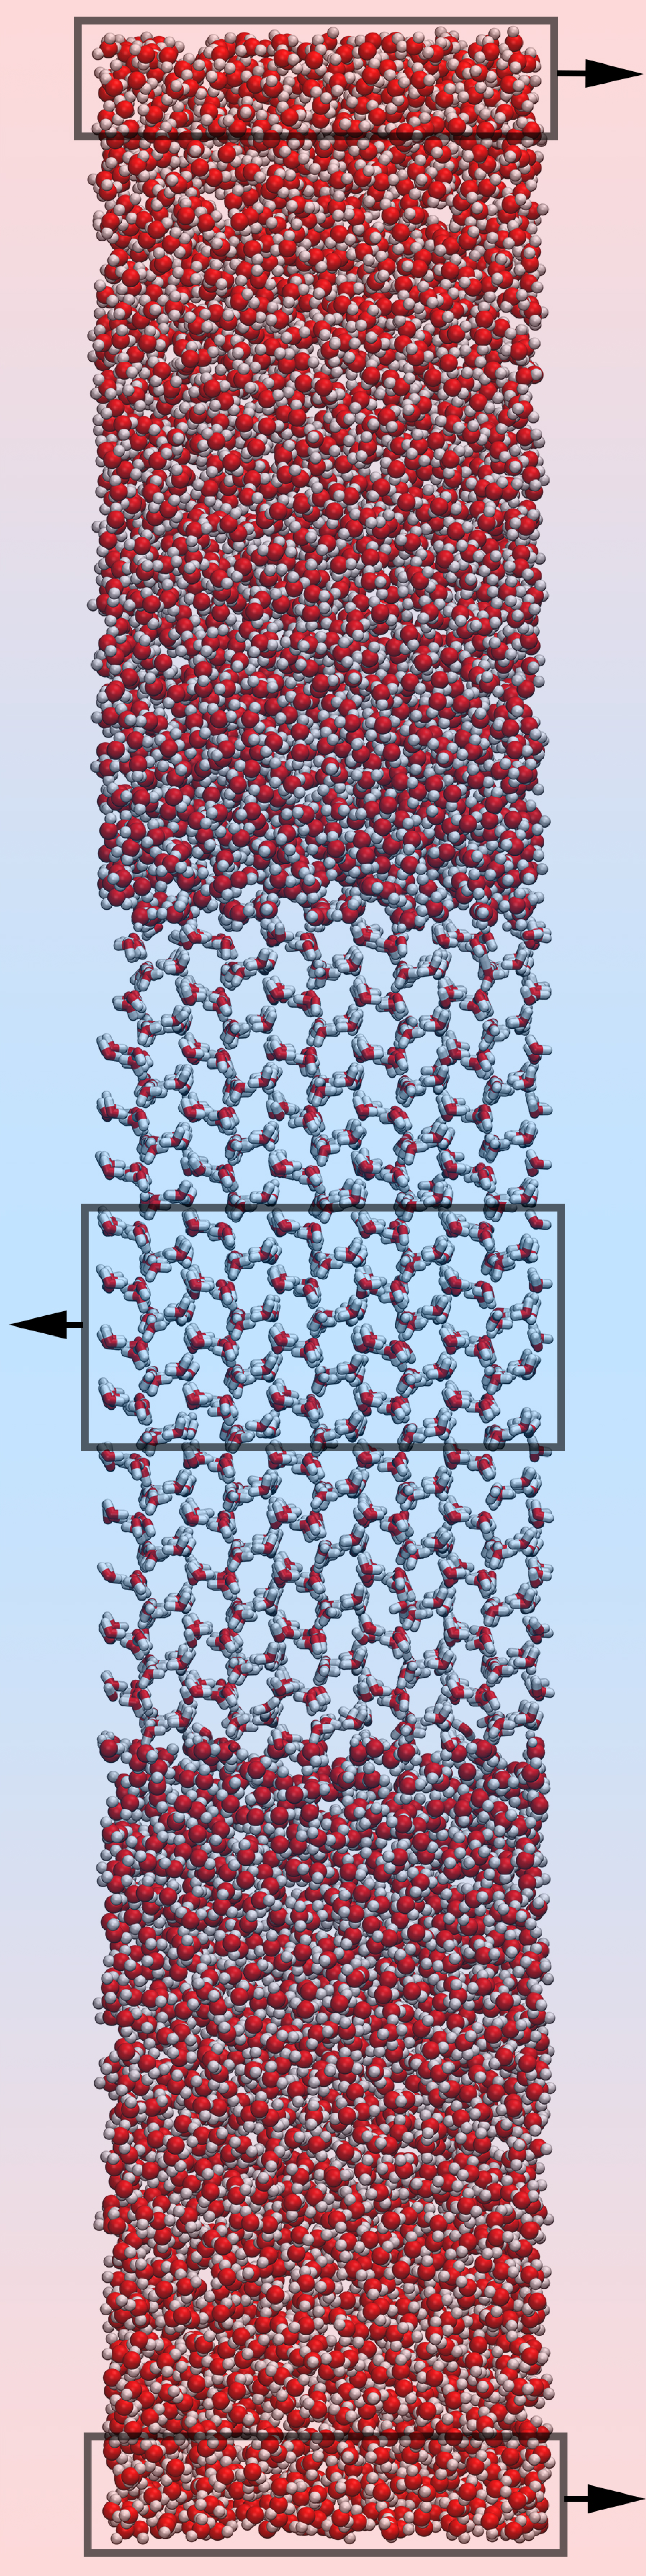
\includegraphics[width=1.9in]{Figures/Shearing}
\caption{\label{fig:Shearing} Computational model of a slab of ice
  being sheared through liquid water.  The ice presents two copies of
  the prismatic $\{10\bar{1}0\}$ facet towards the liquid phase.  The
  RNEMD simulation exchanges both linear momentum (indicated with
  arrows) and kinetic energy between the central box and the box that
  spans the cell boundary.  The system responds with weak thermal
  gradient and a velocity profile that shears the ice relative to the
  surrounding liquid.}
\end{figure}

\section{Computational Details}
All simulations were performed using OpenMD,\cite{OOPSE,openmd} with a
time step of 2 fs and periodic boundary conditions in all three
dimensions.  Electrostatics were handled using the damped-shifted
force real-space electrostatic kernel.\cite{Ewald} When applicable,
VSS-RNEMD moves were attempted every time step. This minimized the
magnitude of individual momentum exchanges.  Forcefield parameters for
both water models can be found in table \ref{tab:waterModels}.

\begin{table}[H]
\centering
\caption{Forcefield parameters for the SPC/E and TIP4P/Ice water
  models.}
\label{tab:waterModels}
\begin{tabular}{|l|c|c|c|c|c|c|c|c|} 
\hline
  Model &  $\sigma$ (\AA) & $\epsilon$ (kJ $\mathrm{mol}^{-2}$) &
                                                              $\mathrm{l}_{1}$
                                                              (\AA) &
                                                                    $\mathrm{l}_{2}$
                                                                      (\AA)
  & $\mathrm{q}_{1}$ (e) & $\mathrm{q}_{2}$ (e) & $\theta$
                                                  ($^{\mathrm{o}}$) &
                                                                      $\phi$ ($^{\mathrm{o}}$) \\ \hline
  SPC/E & 3.166 & 0.650 & 1.000 & - & +0.4238 & -0.8476 & 109.47 & - \\
  TIP4P/Ice & 3.1668 & 0.8822 & 0.9572 & 0.1577 & +0.5897 & -1.1794 &
  104.52 & 52.26 \\
\hline
\end{tabular}
\end {table}


The interfaces were equilibrated for a total of 10 ns at equilibrium
conditions before being exposed to either a shear or thermal gradient.
This consisted of 5 ns under a constant temperature (NVT) integrator
set to 225K followed by 5 ns under a microcanonical integrator.  Weak
thermal gradients were allowed to develop using the VSS-RNEMD (NVE)
integrator using a small thermal flux ($-2.0\times 10^{-6}$
kcal/mol/\AA$^2$/fs) for a duration of 5 ns to allow the gradient to
stabilize.  The resulting thermal gradients ($< 10$~K over the length
of the simulation box) were allowed to stabilize for 5 ns, and were
found to be sufficient to keep the interface within $\pm 5$ K of the
target temperature (225~K for SPC/E and 270~K for TIP4P/Ice) during
all shearing simulations.


Velocity gradients were then imposed using the VSS-RNEMD (NVE)
integrator with a range of momentum fluxes.  These gradients were
allowed to stabilize for 1~ns before data collection began. Once
established, four successive 0.5~ns runs were performed for each shear
rate.  During these simulations, snapshots of the system were taken
every 1~ps, and statistics on the structure and dynamics in each bin
were accumulated throughout the simulations.  Although there was some
small variation in the measured interfacial width between succcessive
runs, no indication of bulk melting (or crystallization) was observed.





% \section{Results and discussion}

% \subsection{Interfacial width}
% Any order parameter or time correlation function that changes as one
% crosses an interface from a bulk liquid to a solid can be used to
% measure the width of the interface.  In previous work on the ice/water
% interface, Haymet {\it et al.}\cite{Bryk02} have utilized structural
% features (including the density) as well as dynamic properties
% (including the diffusion constant) to estimate the width of the
% interfaces for a number of facets of the ice crystals.  Because
% VSS-RNEMD imposes a lateral flow, parameters that depend on
% translational motion of the molecules (e.g. diffusion) may be
% artificially skewed by the RNEMD moves.  A structural parameter is not
% influenced by the RNEMD perturbations to the same degree. Here, we
% have used the local tetrahedral order parameter as described by
% Kumar\cite{Kumar09} and Errington\cite{Errington01} as our principal
% measure of the interfacial width.  A previous study by Bryk and Haymet
% also used local tetrahedrality as an order parameter for ice/water
% interfaces.\cite{Bryk2004b}

% The local tetrahedral order parameter, $q(z)$, is given by
% \begin{equation}
% q(z) = \int_0^L \sum_{k=1}^{N} \Bigg(1 -\frac{3}{8}\sum_{i=1}^{3}
% \sum_{j=i+1}^{4} \bigg(\cos\psi_{ikj}+\frac{1}{3}\bigg)^2\Bigg)
% \delta(z_{k}-z)\mathrm{d}z \Bigg/ N_z
% \label{eq:qz}
% \end{equation}
% where $\psi_{ikj}$ is the angle formed between the oxygen site on
% central molecule $k$, and the oxygen sites on two of the four closest
% molecules, $i$ and $j$.  Molecules $i$ and $j$ are further restricted
% to lie withing the first peak in the pair distribution function for
% molecule $k$ (typically $<$ 3.41 \AA\ for water).  $N_z = \int
% \delta(z_k - z) \mathrm{d}z$ is a normalization factor to account for
% the varying population of molecules within each finite-width bin.  The
% local tetrahedral order parameter has a range of $(0,1)$, where the
% larger values of $q$ indicate a larger degree of tetrahedral ordering
% of the local environment.  In perfect ice I$_\mathrm{h}$ structures,
% the parameter can approach 1 at low temperatures, while in liquid
% water, the ordering is significantly less tetrahedral, and values of
% $q(z) \approx 0.75$ are more common.

% To estimate the interfacial width, the system was divided into 100
% bins along the $z$-dimension.  The $q_{z}$ function was time-averaged
% to give yield a tetrahedrality profile of the system. The profile was
% then fit to a hyperbolic tangent that smoothly links the liquid and
% solid states,
% \begin{equation}\label{tet_fit}
% q(z) \approx
% q_{liq}+\frac{q_{ice}-q_{liq}}{2}\left[\tanh\left(\frac{z-l}{w}\right)-\tanh\left(\frac{z-r}{w}\right)\right]+\beta\left|z-
% \frac{r+l}{2}\right|.
% \end{equation}
% Here $q_{liq}$ and $q_{ice}$ are the local tetrahedral order parameter
% for the bulk liquid and ice domains, respectively, $w$ is the width of
% the interface.  $l$ and $r$ are the midpoints of the left and right
% interfaces, respectively.  The last term in eq. \eqref{tet_fit}
% accounts for the influence that the weak thermal gradient has on the
% tetrahedrality profile in the liquid region. 

% In Figures \ref{fig:bComic} and \ref{fig:pComic} we see the
% $z$-coordinate profiles for tetrahedrality, temperature, and the
% $x$-component of the velocity for the basal and prismatic interfaces.
% The lower panels show the $q(z)$ (black circles) along with the
% hyperbolic tangent fits (red lines). In the liquid region, the local
% tetrahedral order parameter, $q(z) \approx 0.75$ while in the
% crystalline region, $q(z) \approx 0.94$, indicating a more tetrahedral
% environment.  The vertical dotted lines denote the midpoint of the
% interfaces ($r$ and $l$ in eq. \eqref{tet_fit}). The weak thermal
% gradient applied to the systems in order to keep the interface at
% 225~$\pm$~5K, can be seen in middle panels.  The transverse velocity
% profile is shown in the upper panels.  It is clear from the upper
% panels that water molecules in close proximity to the surface (i.e.
% within 10~\AA\ to 15~\AA~of the interfaces) have transverse velocities
% quite close to the velocities within the ice block.  There is no
% velocity discontinuity at the interface, which indicates that the
% shearing of ice/water interfaces occurs in the ``stick'' or no-slip
% boundary conditions.

% \begin{figure}
% 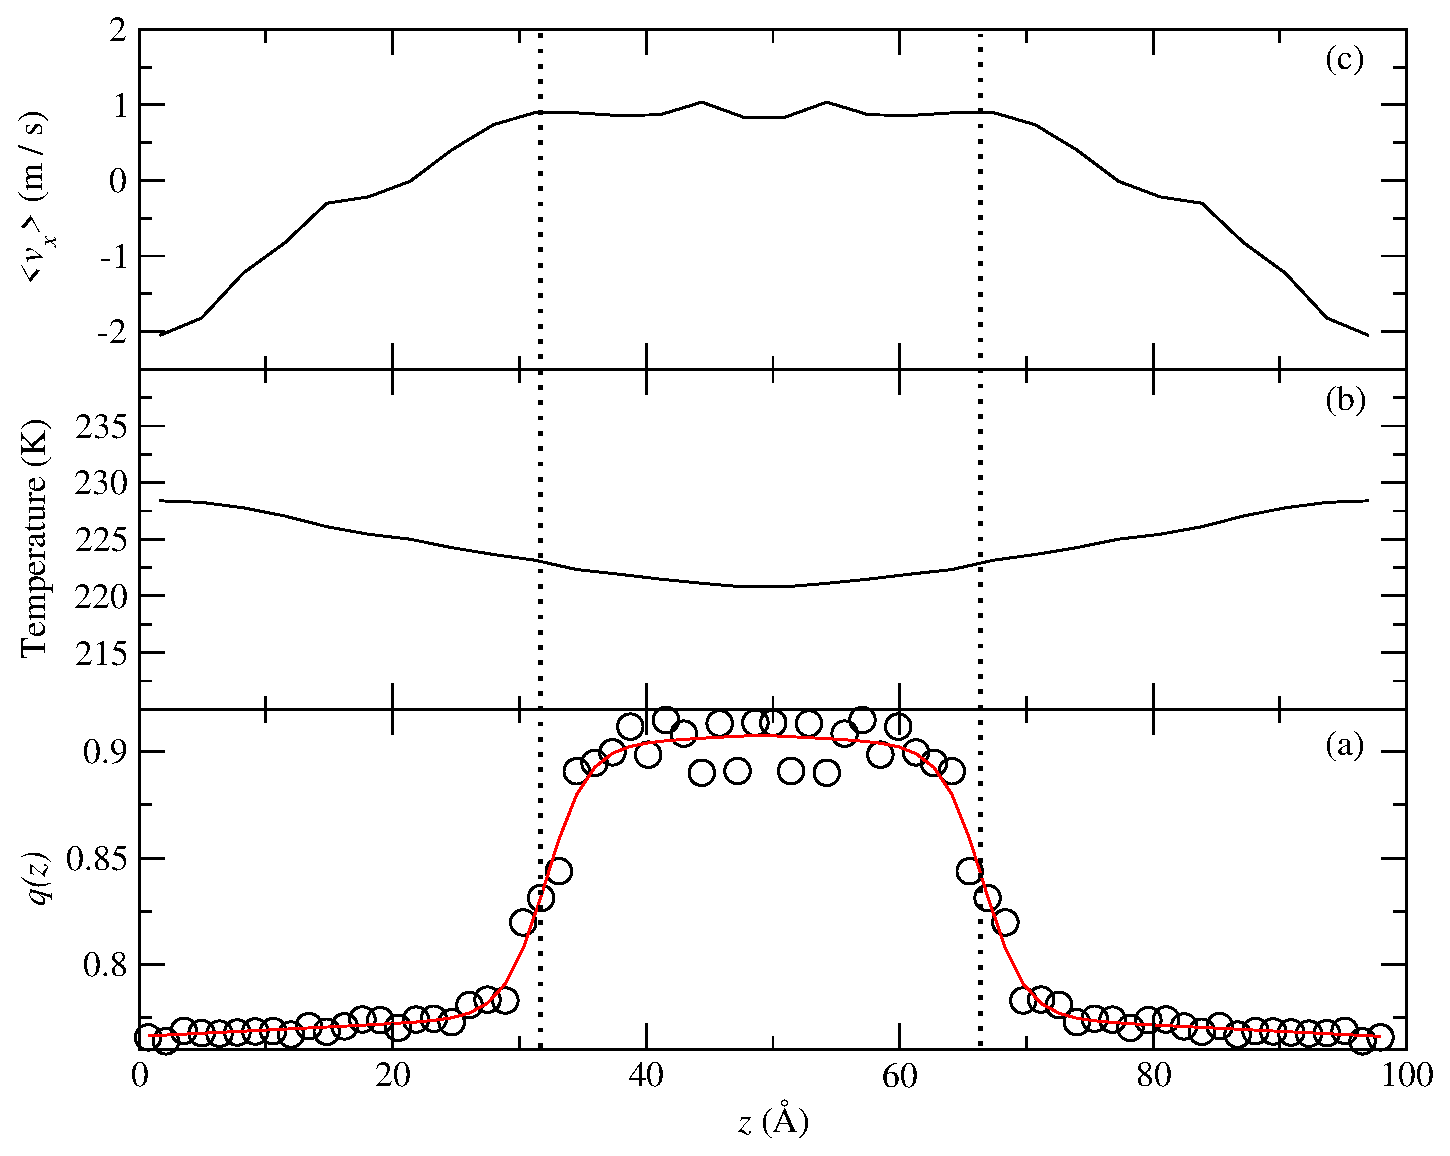
\includegraphics[width=\linewidth]{Figures/bComicStrip}
% \caption{\label{fig:bComic} The basal interface with a shear rate of
%   1.3 ms\textsuperscript{-1}.  Lower panel: the local tetrahedral order parameter, $q(z)$,
%   (black circles) and the hyperbolic tangent fit (red line).  Middle
%   panel: the imposed thermal gradient required to maintain a fixed
%   interfacial temperature.  Upper panel: the transverse velocity
%   gradient that develops in response to an imposed momentum flux.  The
%   vertical dotted lines indicate the locations of the midpoints of the
%   two interfaces.}
% \end{figure}

% \begin{figure}
% 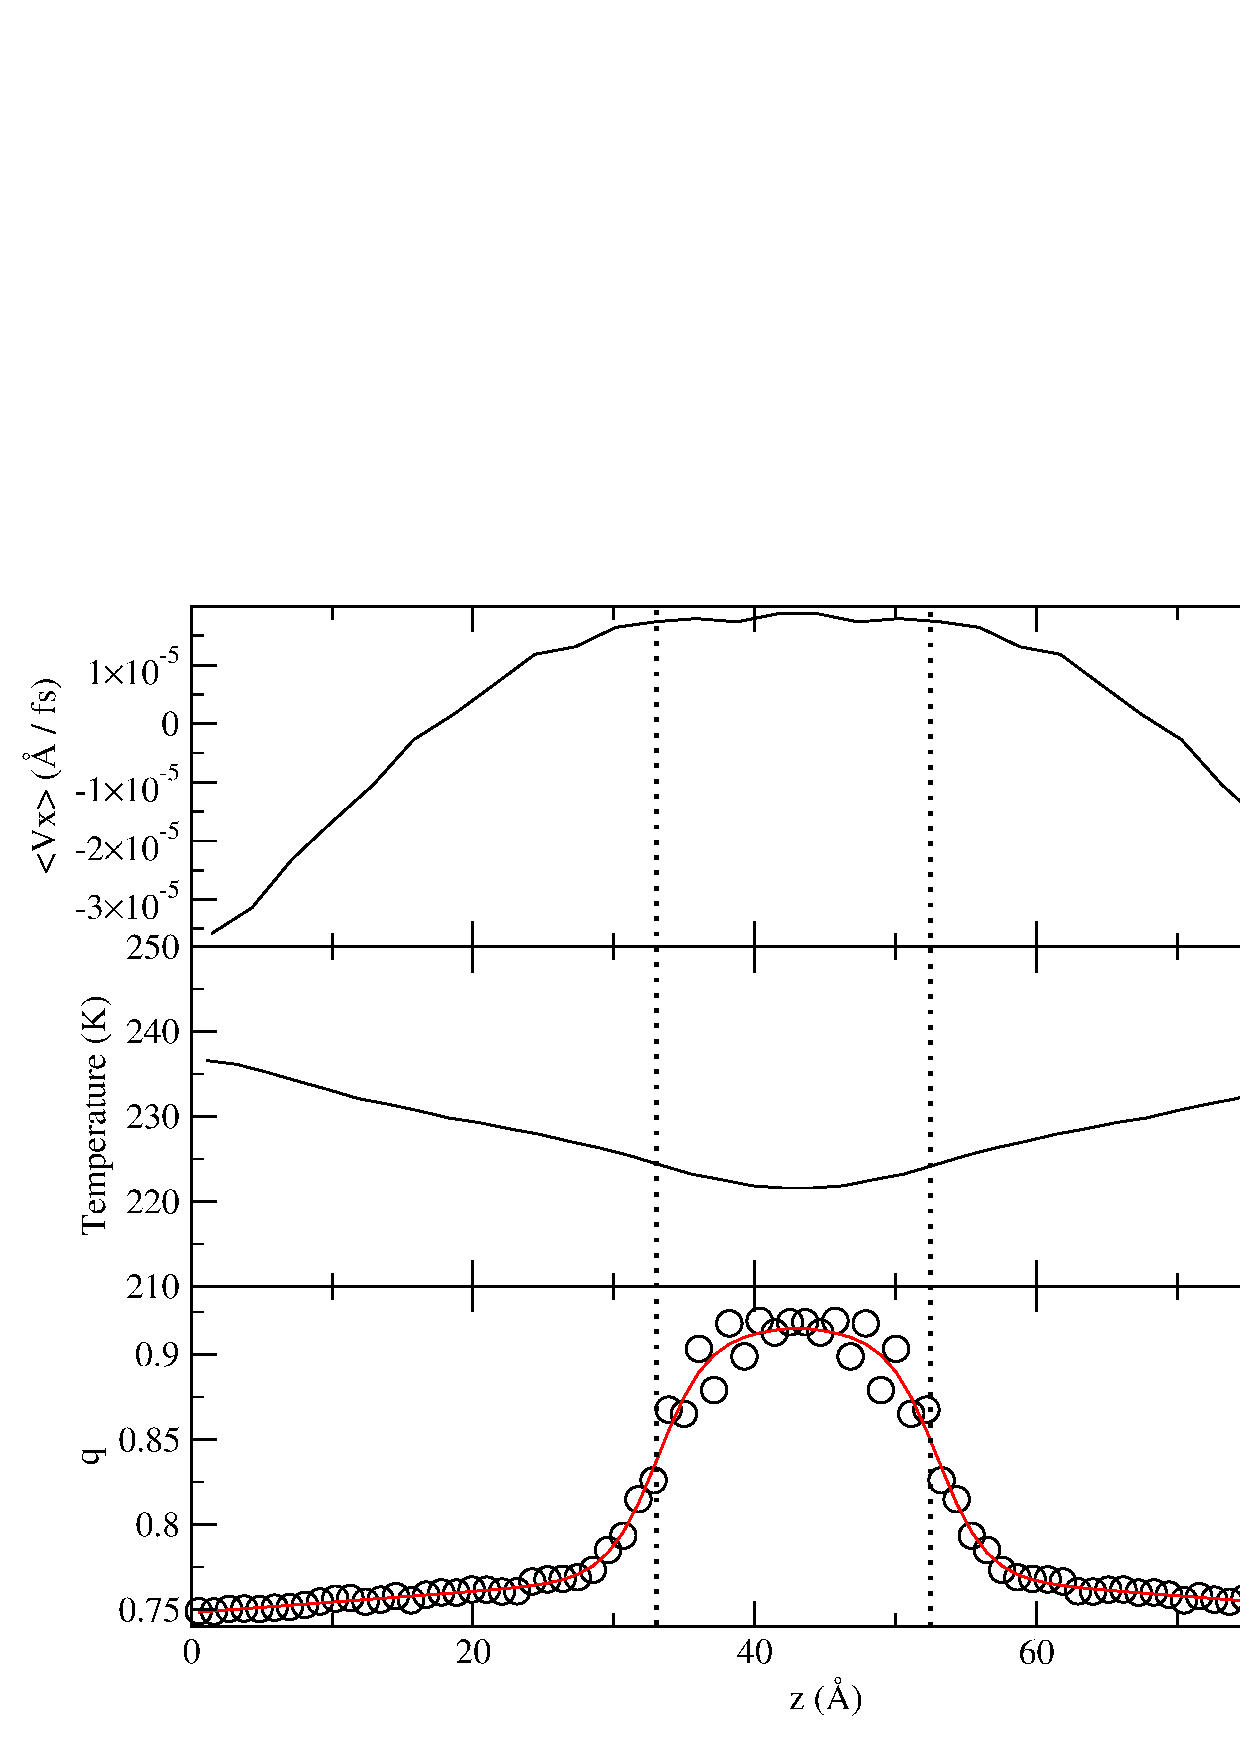
\includegraphics[width=\linewidth]{Figures/pComicStrip}
% \caption{\label{fig:pComic} The prismatic interface with a shear rate
%   of 2.0 ms\textsuperscript{-1}.  Panel
%   descriptions match those in figure \ref{fig:bComic}}
% \end{figure}

% From the fits using eq. \eqref{tet_fit}, we find the interfacial width
% for the basal and prismatic systems to be 3.2~$\pm$~0.4~\AA\ and
% 3.6~$\pm$~0.2~\AA\ , respectively, with no applied momentum flux. Over
% the range of shear rates investigated, $0.6 \pm 0.3 \mathrm{ms}^{-1}
% \rightarrow 5.3 \pm 0.5 \mathrm{ms}^{-1}$ for the basal system and
% $0.9 \pm 0.2 \mathrm{ms}^{-1} \rightarrow 4.5 \pm 0.1
% \mathrm{ms}^{-1}$ for the prismatic, we found no appreciable change in
% the interface width. The fit values for the interfacial width ($w$)
% over all shear rates contained the values reported above within their
% error bars.  Note that the interfacial widths reported here are based
% on the hyperbolic tangent parameter $w$ in Eq. \ref{tet_fit}.  This is
% related to, but not identical with, the 10\%-90\% intefacial widths
% commonly used in previous studies.\cite{Bryk02,Bryk2004b} To estimate
% the 10\%-90\% widths, it is a simple matter to scale the widths
% obtained from the hyperbolic tangent fits to obtain $w_{10-90} =
% 2.1971 \times w$.\cite{Bryk02,Bryk2004b} This results in $w_{10-90}$
% values of 7.0~$\pm$~0.9~\AA\ for the basal face, and 7.9~$\pm$~0.4
% \AA\ for the prismatic face.  These are somewhat smaller than
% previously reported values.

% \begin{figure}
% 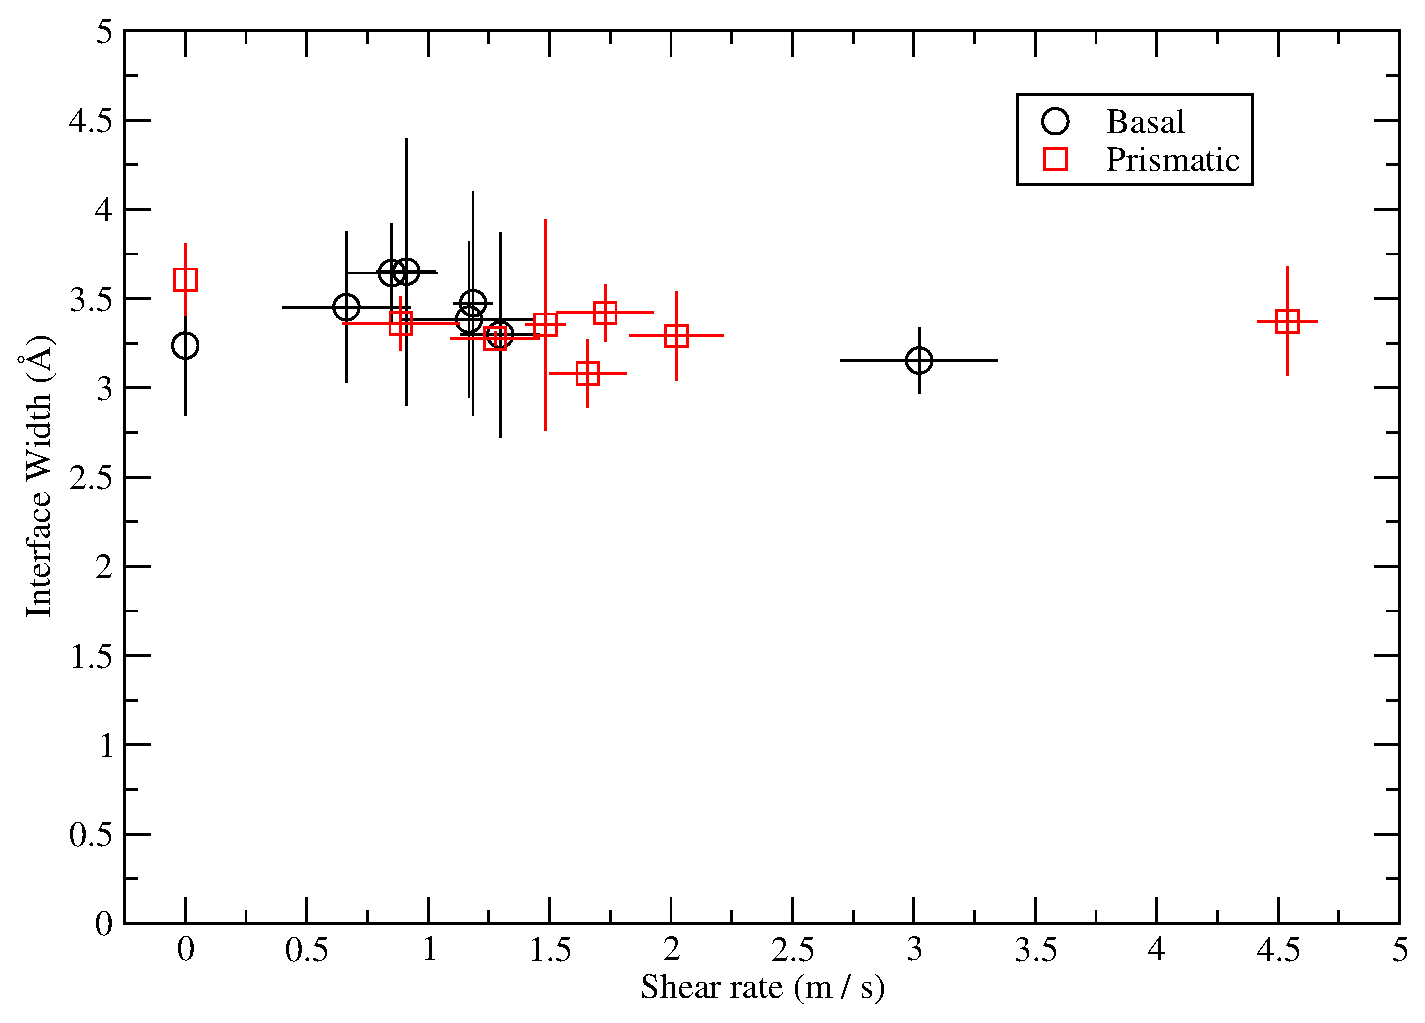
\includegraphics[width=\linewidth]{Figures/interface_width_by_shear_rate}
% \caption{\label{fig:widthByShear} The width of the ice water
%   interfaces (as measured by Eq. \ref{tet_fit}) exhibits no dependence
%   on the applied shear rate between the ice and water regions.}
% \end{figure}



% \subsubsection{Orientational Dynamics}
% The orientational time correlation function,
% \begin{equation}\label{C(t)1}
%   C_{2}(t)=\langle P_{2}(\mathbf{u}(0) \cdot \mathbf{u}(t)) \rangle,
% \end{equation}
% gives insight into the local dynamic environment around the water
% molecules.  The rate at which the function decays provides information
% about hindered motions and the timescales for relaxation.  In
% eq. \eqref{C(t)1}, $P_{2}$ is the second-order Legendre polynomial,
% the vector $\mathbf{u}$ is often taken as HOH bisector, although
% slightly different behavior can be observed when $\mathbf{u}$ is the
% vector along one of the OH bonds.  The angle brackets denote an
% ensemble average over all water molecules in a given spatial region.

% To investigate the dynamic behavior of water at the ice interfaces, we
% have computed $C_{2}(z,t)$ for molecules that are present within a
% particular slab along the $z$- axis at the initial time.  The change
% in the decay behavior as a function of the $z$ coordinate is another
% measure of the change of how the local environment changes across the
% ice/water interface.  To compute these correlation functions, each of
% the 0.5 ns simulations was followed by a shorter 200 ps microcanonical
% (NVE) simulation in which the positions and orientations of every
% molecule in the system were recorded every 0.1 ps. The systems were
% then divided into 30 bins along the $z$-axis and $C_2(t)$ was
% evaluated for each bin.

% In simulations of water at biological interfaces, Furse {\em et al.}
% fit $C_2(t)$ functions for water with triexponential
% functions,\cite{Furse08} where the three components of the decay
% correspond to a fast ($<$200 fs) reorientational piece driven by the
% restoring forces of existing hydrogen bonds, a middle (on the order of
% several ps) piece describing the large angle jumps that occur during
% the breaking and formation of new hydrogen bonds,and a slow (on the
% order of tens of ps) contribution describing the translational motion
% of the molecules.  The model for orientational decay presented
% recently by Laage and Hynes {\em et al.}\cite{Laage08,Laage11} also
% includes three similar decay constants, although two of the time
% constants are linked, and the resulting decay curve has two parameters
% governing the dynamics of decay. 

% In our ice/water interfaces, we are at substantially lower
% temperatures, and the water molecules are further perturbed by the
% presence of the ice phase nearby.  We have obtained the most
% reasonable fits using triexponential functions with three distinct
% time domains, as well as a constant piece to account for the water
% stuck in the ice phase that does not experience any long-time
% orientational decay,
% \begin{equation}
% C_{2}(t) \approx a e^{-t/\tau_\mathrm{short}} + b e^{-t/\tau_\mathrm{middle}} + c
% e^{-t/\tau_\mathrm{long}} + (1-a-b-c)
% \end{equation}
% Average values for the three decay constants (and error estimates)
% were obtained for each bin. In figures \ref{fig:basal_Tau_comic_strip}
% and \ref{fig:prismatic_Tau_comic_strip}, the three orientational decay
% times are shown as a function of distance from the center of the ice
% slab.

% \begin{figure}
% 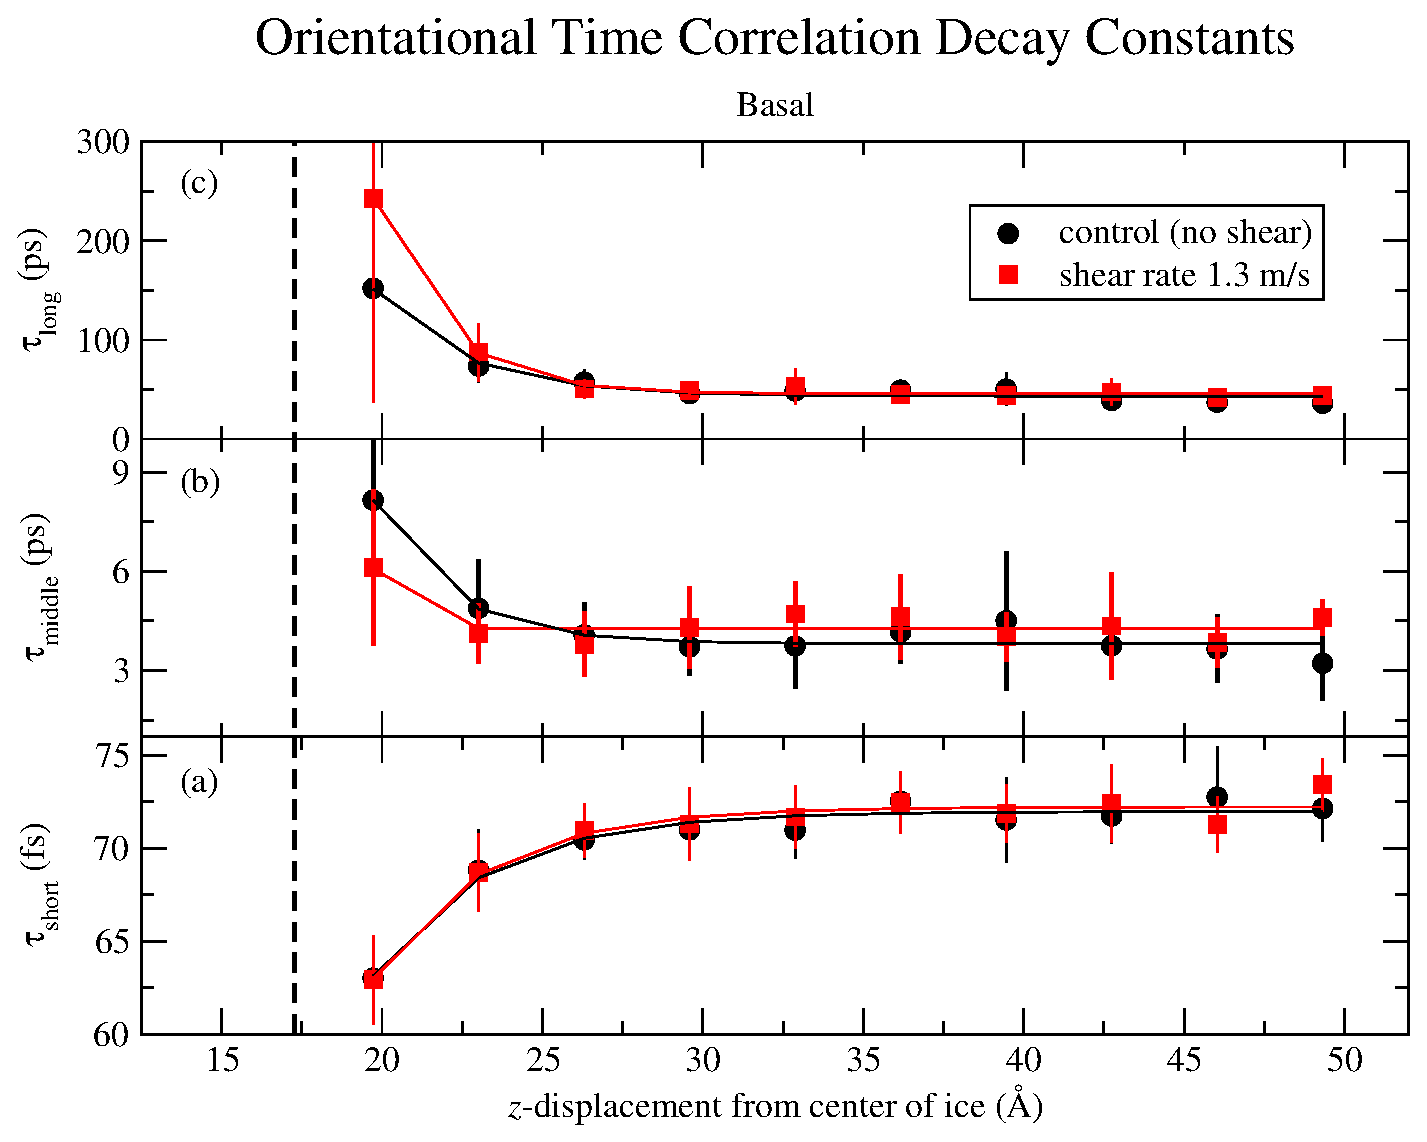
\includegraphics[width=\linewidth]{Figures/basal_Tau_comic_strip}
% \caption{\label{fig:basal_Tau_comic_strip} The three decay constants
%   of the orientational time correlation function, $C_2(t)$, for water
%   as a function of distance from the center of the ice slab.  The
%   dashed line indicates the location of the basal face (as determined
%   from the tetrahedrality order parameter) and the black and red lines
%   are fits of Eq. \ref{tauFit}.  The moderate and long
%   time contributions slow down close to the interface which would be
%   expected under reorganizations that involve large motions of the
%   molecules (e.g. frame-reorientations and jumps).  The observed
%   speed-up in the short time contribution is surprising, but appears
%   to reflect the restricted motion of librations closer to the
%   interface.}
% \end{figure}

% \begin{figure}
% 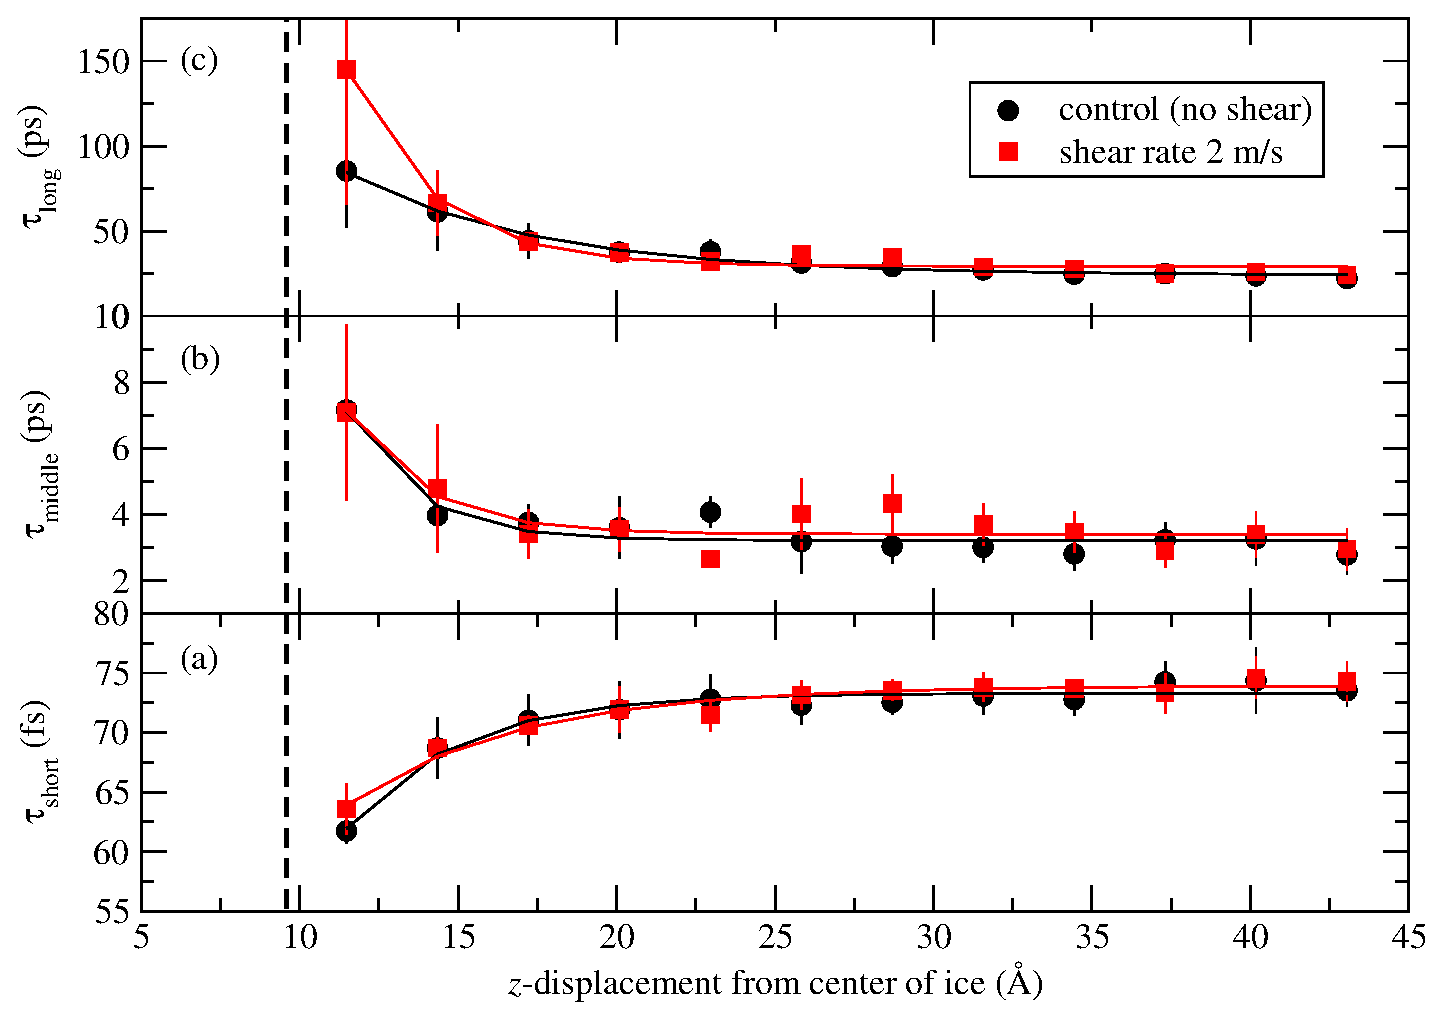
\includegraphics[width=\linewidth]{Figures/prismatic_Tau_comic_strip}
% \caption{\label{fig:prismatic_Tau_comic_strip}
%  Decay constants for $C_2(t)$ at the prismatic interface.  Panel
%   descriptions match those in figure \ref{fig:basal_Tau_comic_strip}.}
% \end{figure}

% Figures \ref{fig:basal_Tau_comic_strip} and
% \ref{fig:prismatic_Tau_comic_strip} show the three decay constants for
% the orientational time correlation function for water at varying
% displacements from the center of the ice slab for both the basal and
% prismatic interfaces.  The vertical dotted lines indicate the
% locations of the midpoints of the interfaces as determined by the
% tetrahedrality fits. In the liquid regions, $\tau_{middle}$ and
% $\tau_{long}$ have consistent values around 3-4 ps and 20-40 ps,
% respectively, and increase in value approaching the interface.
% According to the jump model of Laage and Hynes {\em et
%   al.},\cite{Laage08,Laage11} $\tau_{middle}$ corresponds to the
% breaking and making of hydrogen bonds and $\tau_{long}$ is explained
% with translational motion of the molecules (i.e. frame reorientation).
% The shortest of the three decay constants, the librational time
% $\tau_\mathrm{short}$ has a value of about 70 fs in the liquid region,
% and decreases in value approaching the interface. The observed
% speed-up in the short time contribution is surprising, but appears to
% reflect the restricted motion of librations closer to the interface.

% The control systems (with no applied momentum flux) are shown with
% black symbols in figs. \ref{fig:basal_Tau_comic_strip} and
% \ref{fig:prismatic_Tau_comic_strip}, while those obtained while a
% shear was active are shown in red.

% Two notable features deserve clarification.  First, there are
% nearly-constant liquid-state values for $\tau_{short}$,
% $\tau_{middle}$, and $\tau_{long}$ at large displacements from the
% interface. Second, there appears to be a single distance, $d_{basal}$
% or $d_{prismatic}$, from the interface at which all three decay times
% begin to deviate from their bulk liquid values. To quantify this
% distance, each of the decay constant $z$-profiles were fit to
% \begin{equation}\label{tauFit}
% \tau(z)\approx\tau_{liquid}+(\tau_{solid}-\tau_{liquid})e^{-(z-z_{wall})/d}
% \end{equation}
% where $\tau_{liquid}$ and $\tau_{solid}$ are the liquid and projected
% solid values of the decay constants, $z_{wall}$ is the location of the
% interface, and $d$ is the displacement the deviations occur at (see
% Figures \ref{fig:basal_Tau_comic_strip} and
% \ref{fig:prismatic_Tau_comic_strip}). The displacements $d_{basal}$
% and $d_{prismatic}$ were determined for each of the three decay
% constants, and then averaged for better statistics.
% For the basal system, we found $d_{basal}$ for the control set to be
% 2.9 \AA\, and 2.8 \AA\ for a simulation with a shear rate of 1.3
% ms\textsuperscript{-1}. We found $d_{prismatic}$ to be slightly
% larger than $d_{basal}$ for both the control and an applied shear,
% with displacements of 3.6 \AA\ for the control system and 3.5 \AA\ for
% a simulation with a 2 ms\textsuperscript{-1} shear rate. From this we
% can conclude there is no apparent dependence on the shear rate for the dynamic interface
% width. 

% %%%%%%%%Should we keep this paragraph???%%%%%%%%%%%%%%%
% Beaglehole and Wilson have measured the ice/water interface using
% ellipsometry and find a thickness of approximately 10~\AA\ for both
% the basal and prismatic faces.\cite{Beaglehole93} Structurally, we
% have found the basal and prismatic interfacial width to be
% 3.2~$\pm$~0.4~\AA\ and 3.6~$\pm$~0.2~\AA.  Decomposition of
% the spatial dependence of the decay times of $C_2(t)$ shows good
% agreement with the structural interfacial width determined by the
% local tetrahedrality.
% %%%%%%%%%%%%%%%%%%%%%%%%%%%%%%%%%%%%%%%%%%%%%%


% \subsection{Coefficient of Friction of the Interface}
% As liquid water flows over an ice interface, there is a distance from
% the structural interface where bulk-like hydrodynamics are recovered.
% Bocquet and Barrat constructed a theory for the hydrodynamic boundary
% parameters, which include the slipping length
% $\left(\delta_\mathrm{wall}\right)$ of this boundary layer and the
% ``hydrodynamic position'' of the boundary
% $\left(z_\mathrm{wall}\right)$.\cite{PhysRevLett.70.2726,PhysRevE.49.3079}
% This last parameter is the location (relative to a solid surface)
% where the bulk-like behavior is recovered.  Work by Mundy {\it et al.}
% has helped to combine these parameters into a liquid-solid friction
% coefficient, which quantifies the resistance to pulling the solid
% interface through a liquid,\cite{Mundy1997305}
% \begin{equation}
% \lambda_\mathrm{wall} = \frac{\eta}{\delta_\mathrm{wall}}.
% \end{equation}
% This expression is nearly identical to one provided by Pit {\it et
%   al.} for the solid-liquid friction of an interface,\cite{Pit99}
% \begin{equation}\label{Pit}
%   \lambda=\frac{\eta}{\delta}
% \end{equation}
% where $\delta$ is the slip length for the liquid measured at the
% location of the interface itself.  In our simulations, the shoulder on
% the velocity profile indicating the location of the hydrodynamic
% boundary in the liquid is not always apparent. In some cases, the
% linear behavior persists nearly up to the interfacial region.  For
% this reason, the hydrodynamic position of the boundary is not always
% computable, while the Pit approach (Eq. \ref{Pit}) can be used to find
% the solid-liquid friction coefficient more reliably.

% In both the Pit and hydrodynamic boundary expressions, $\eta$ is the
% shear viscosity of the bulk-like region of the liquid, a quantity
% which is easily obtained in VSS-RNEMD simulations by fitting the
% velocity profile in the region far from the surface.\cite{Kuang12}
% Assuming linear response in the bulk-like region,
% \begin{equation}\label{Kuang}
% j_{z}(p_{x})=-\eta \left(\frac{\partial v_{x}}{\partial z}\right)
% \end{equation}
% Substituting this result into eq. \eqref{Pit}, we can estimate the
% solid-liquid coefficient using the slip length,
% \begin{equation}
% \lambda=-\frac{j_{z}(p_{x})} {\left(\frac{\partial v_{x}}{\partial
%       z}\right) \delta}
% \end{equation}

% For ice / water interfaces, the boundary conditions are no-slip, so
% projecting the bulk liquid state velocity profile yields a negative
% slip length. This length is the difference between the structural edge
% of the ice (determined by the tetrahedrality profile) and the location
% where the projected velocity of the bulk liquid intersects the solid
% phase velocity (see Figure \ref{fig:delta_example}). The coefficients
% of friction for the basal and the prismatic facets were determined for
% shearing along both the $x$ and $y$ axes.  The values are given in
% table \ref{tab:lambda}. 

% Note that the measured friction coefficient for the basal face is
% twice that of the prismatic face (regardless of drag direction).
% These results may seem surprising as the basalface appears smoother
% than the prismatic with only small undulations of the oxygen
% positions, while the prismatic surface has deep corrugated channels
% along the $x$ direction in the crystal system used in this work.
% However, the corrugations are relatively thin, and the liquid phase
% water does not appear to populate the channels.  The prismatic face
% therefore effectively presents stripes of solid-phase molecules
% (making up approximately half of the exposed surface area) with nearly
% empty space between them. The interfacial friction appears to be
% independent of the drag direction, so flow parallel to these channels
% does not explain the lower friction of the prismatic face.  A more
% likely explanation is that the effective contact between the liquid
% phase and the prismatic face is reduced by the empty corrugations.  

% \begin{figure}
% 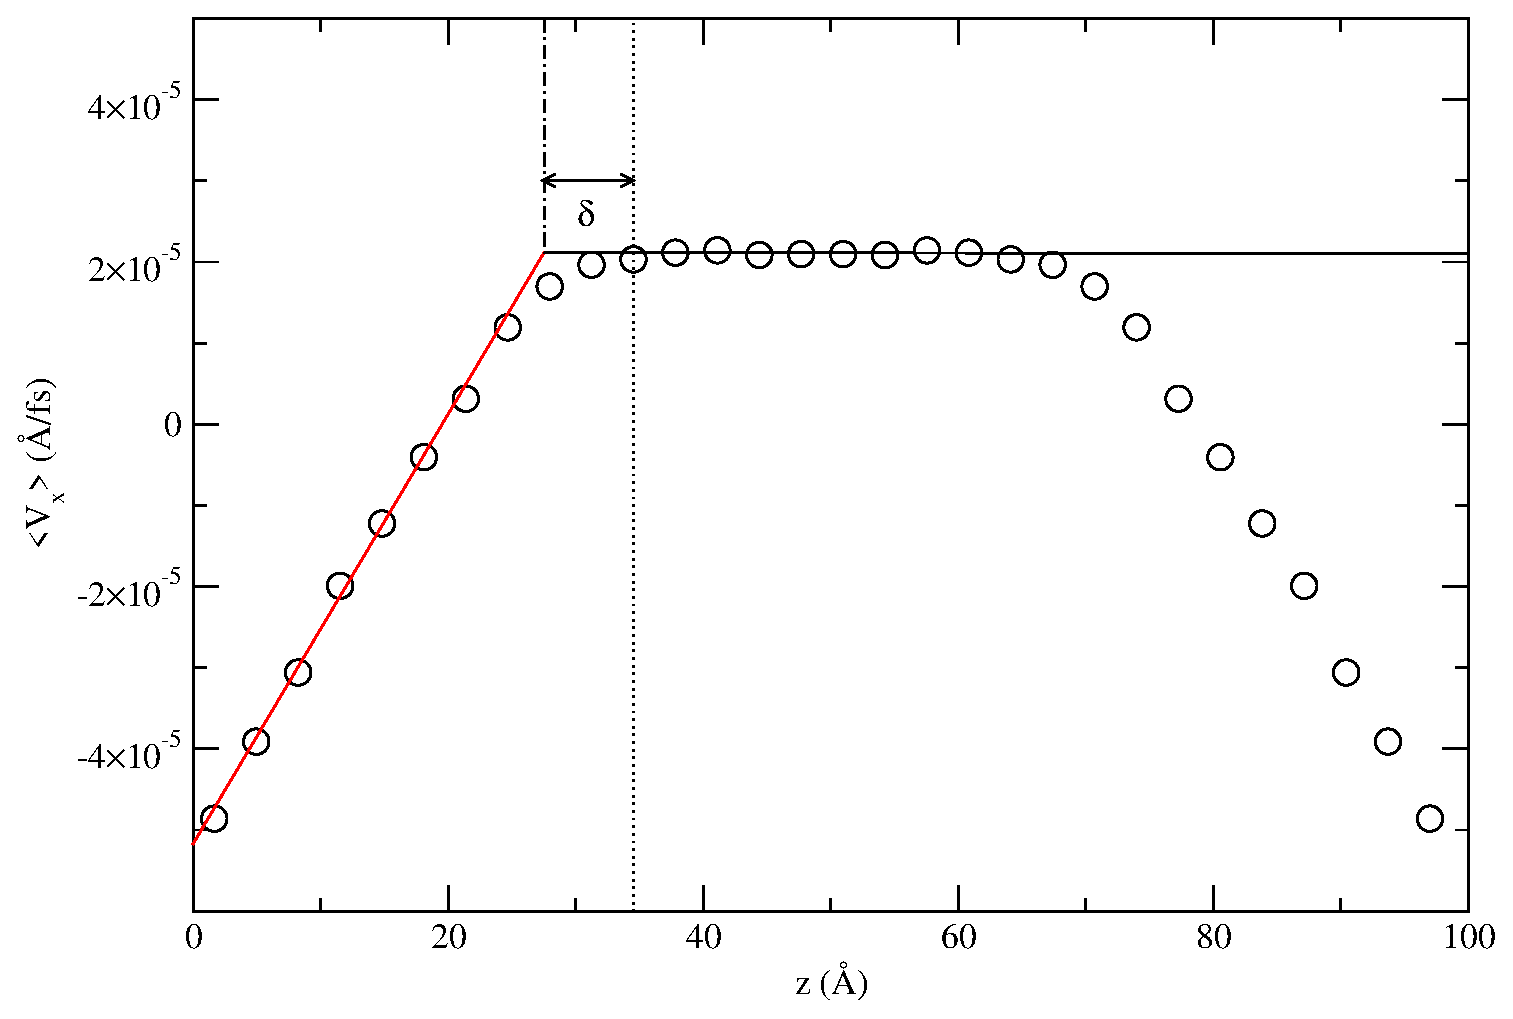
\includegraphics[width=\linewidth]{Figures/delta_example}
% \caption{\label{fig:delta_example} Determining the (negative) slip
%   length ($\delta$) for the ice-water interfaces (which have decidedly
%   non-slip behavior).  This length is the difference between the
%   structural edge of the ice (determined by the tetrahedrality
%   profile) and the location where the projected velocity of the bulk
%   liquid (dashed red line) intersects the solid phase velocity (solid
%   black line).  The dotted line indicates the location of the ice as
%   determined by the tetrahedrality profile.  This example is taken
%   from the basal-face simulation with an applied shear rate of 3.0 ms\textsuperscript{-1}.}
% \end{figure}


% \begin{table}[h]
% \centering
% \caption{Solid-liquid friction coefficients (measured in amu~fs\textsuperscript{-1}) }
% \label{tab:lambda}
% \begin{tabular}{|ccc|}  \hline
%            & \multicolumn{2}{c|}{Drag direction} \\ 
%  Interface & $x$               & $y$  \\ \hline
%      basal &  $0.08 \pm 0.02$  & $0.09 \pm 0.03$ \\
%  prismatic & $0.037 \pm 0.008$ & $0.04 \pm 0.01$ \\ \hline
% \end{tabular}
% \end{table}


% \section{Conclusion}
% We have simulated the basal and prismatic facets of an SPC/E model of
% the ice I$_\mathrm{h}$ / water interface.  Using VSS-RNEMD, the ice
% was sheared relative to the liquid while simultaneously being exposed
% to a weak thermal gradient which kept the interface at a stable
% temperature.  Calculation of the local tetrahedrality order parameter
% has shown an apparent independence of the interfacial width on the
% shear rate.  This width was found to be 3.2~$\pm$0.4~\AA\ and
% 3.6~$\pm$0.2~\AA\ for the basal and prismatic systems, respectively.

% Orientational time correlation functions were calculated at varying
% displacements from the interface, and were found to be similarly
% independent of the applied momentum flux. The short decay due to the
% restoring forces of existing hydrogen bonds decreased close to the
% interface, while the longer-time decay constants increased in close
% proximity to the interface.  There is also an apparent dynamic
% interface width, $d_{basal}$ and $d_{prismatic}$, at which these
% deviations from bulk liquid values begin.  We found $d_{basal}$ and
% $d_{prismatic}$ to be approximately 2.8~\AA\ and 3.5~\AA\ . This
% interfacial width is in good agreement with values determined by the
% structural analysis of the interface, by the hyperbolic tangent fit of
% the local tetrahedral order parameter.

% The coefficient of liquid-solid friction for each of the facets was
% also determined. They were found to be
% 0.07~$\pm$~0.01~amu~fs\textsuperscript{-1} and
% 0.032~$\pm$~0.007~amu~fs\textsuperscript{-1} for the basal and
% prismatic facets respectively. We attribute the large difference
% between the two friction coefficients to the direction of the shear
% and to the surface structure of the crystal facets.




%%%%%%%%%%%%%%%%%%%%%%%%%%%%%%%%%%%%%%%%%%%%%%%%%%%%%%%%%%%%%%%%%%%%%%%%%%%%%%%%%%%
%		CHAPTER 3 -- STRUCTURAL MEASURES OF INT. WIDTH
%%%%%%%%%%%%%%%%%%%%%%%%%%%%%%%%%%%%%%%%%%%%%%%%%%%%%%%%%%%%%%%%%%%%%%%%%%%%%%%%%%%
\chapter{STRUCTURAL WIDTHS OF ICE-I$_\mathrm{h}$ / WATER INTERFACES}

%%%%%%%%%%%%%%%%%%%%%%%%%%%%%%%%%%%%%%%%%%%%%%%%%%%%%%%%%%%%%%%%%%%%%%%%%%%%%%%%%%%
%		CHAPTER 4 -- DYNAMIC MEASURES OF INT. WIDTH
%%%%%%%%%%%%%%%%%%%%%%%%%%%%%%%%%%%%%%%%%%%%%%%%%%%%%%%%%%%%%%%%%%%%%%%%%%%%%%%%%%%
\chapter{DYNAMIC WIDTHS OF ICE-I$_\mathrm{h}$ / WATER INTERFACES}

%%%%%%%%%%%%%%%%%%%%%%%%%%%%%%%%%%%%%%%%%%%%%%%%%%%%%%%%%%%%%%%%%%%%%%%%%%%%%%%%%%%
%		CHAPTER 5 -- FRICTION AT ICE / WATER INTERFACES
%%%%%%%%%%%%%%%%%%%%%%%%%%%%%%%%%%%%%%%%%%%%%%%%%%%%%%%%%%%%%%%%%%%%%%%%%%%%%%%%%%%
\chapter{FRICTION AT ICE-I$_\mathrm{h}$ / WATER INTERFACES IS GOVERNED
  BY SOLID / LIQUID HYDROGEN-BONDING}\label{chap:Friction}


\begin{flushright}
\textit{``If there is magic on this planet, it is contained in water.''} \\
-Loren Eiseley (1957) \\
\end{flushright}


% Write a short introduction to the topic discussed in this chapter.
Calculations of solid-liquid friction at ice-I$_\mathrm{h}$ / water
interfaces are presented in this chapter.  An expression for friction
coefficients appropriate for negative slip boundary conditions is
constructed, and the computed friction of these interfaces is found to
be invariant to the shear rate and direction of shear relative to the
surface features. Solid / liquid hydrogen bonds are identified using
local tetrahedral ordering of the water molecules, and the surface
density of these hydrogen bonds is found to directly correlate with
interfacial friction. Surface topography of the investigated crystal
facets at the ice-I$_\mathrm{h}$ / water interface is quantified by
querying mean projected densities. However, the dimensions of the
surface features do not strongly correlate with the obtained friction
coefficients, leading to the conclusion that friciton is dominated by
the density of solid / liquid hydrogen bonds.  Lastly, we present a
simple momentum transmission model using the density of solid / liquid
hydrogen bonds, the shear viscosity of the liquid, and the structural
width of the interface. This model agrees well with our observed
results for both the SPC/E and TIP4P/Ice simulations.
%\end{abstract}



%\section{Coefficient of Friction of the Interface}
% As liquid water flows over an ice interface, there is a distance from
% the structural interface where bulk-like hydrodynamics are recovered.
% Bocquet and Barrat constructed a theory for the hydrodynamic boundary
% parameters, which include the slipping length
% $\left(\delta_\mathrm{wall}\right)$ of this boundary layer and the
% ``hydrodynamic position'' of the boundary
% $\left(z_\mathrm{wall}\right)$.\cite{PhysRevLett.70.2726,PhysRevE.49.3079}
% This last parameter is the location (relative to a solid surface)
% where the bulk-like behavior is recovered.  Work by Mundy {\it et al.}
% has helped to combine these parameters into a liquid-solid friction
% coefficient, which quantifies the resistance to pulling the solid
% interface through a liquid,\cite{Mundy1997305}
% \begin{equation}
% \lambda_\mathrm{wall} = \frac{\eta}{\delta_\mathrm{wall}}.
% \end{equation}
% This expression is nearly identical to one provided by Pit {\it et
%   al.} for the solid-liquid friction of an interface,\cite{Pit1999}
% \begin{equation}\label{Pit}
%   \lambda=\frac{\eta}{\delta}
% \end{equation}
% where $\delta$ is the slip length for the liquid measured at the
% location of the interface itself.  In our simulations, the shoulder on
% the velocity profile indicating the location of the hydrodynamic
% boundary in the liquid is not always apparent. In some cases, the
% linear behavior persists nearly up to the interfacial region.  For
% this reason, the hydrodynamic position of the boundary is not always
% computable, while the Pit approach (Eq. \ref{Pit}) can be used to find
% the solid-liquid friction coefficient more reliably.

% In both the Pit and hydrodynamic boundary expressions, $\eta$ is the
% shear viscosity of the bulk-like region of the liquid, a quantity
% which is easily obtained in VSS-RNEMD simulations by fitting the
% velocity profile in the region far from the surface.\cite{Kuang2012}
% Assuming linear response in the bulk-like region,
% \begin{equation}\label{Kuang}
% j_{z}(p_{x})=-\eta \left(\frac{\partial v_{x}}{\partial z}\right)
% \end{equation}
% Substituting this result into eq. \eqref{Pit}, we can estimate the
% solid-liquid friction coefficient using the slip length,
% \begin{equation}
% \lambda=-\frac{j_{z}(p_{x})} {\left(\frac{\partial v_{x}}{\partial
%       z}\right) \delta}.
% \end{equation}

% For ice / water interfaces, the boundary conditions are no-slip, so
% projecting the bulk liquid state velocity profile yields a negative
% slip length. This length is the difference between the structural edge
% of the ice (determined by the tetrahedrality profile) and the location
% where the projected velocity of the bulk liquid intersects the solid
% phase velocity (see Figure \ref{fig:delta_example}). The coefficients
% of friction for the basal and the prismatic facets were determined for
% shearing along both the $x$ and $y$ axes.  The values are given in
% Table \ref{tab:lambda}. 

% Note that the measured friction coefficient for the basal face is
% twice that of the prismatic face (regardless of drag direction).
% These results may seem surprising as the basal face appears smoother
% than the prismatic with only small undulations of the oxygen
% positions, while the prismatic surface has deep corrugated channels
% along the $x$ direction in the crystal system used in this work.
% However, the corrugations are relatively thin, and the liquid phase
% water does not appear to populate the channels.  The prismatic face
% therefore effectively presents stripes of solid-phase molecules
% (making up approximately half of the exposed surface area) with nearly
% empty space between them. The interfacial friction appears to be
% independent of the drag direction, so flow parallel to these channels
% does not explain the lower friction of the prismatic face.  A more
% likely explanation is that the effective contact between the liquid
% phase and the prismatic face is reduced by the empty corrugations.  


\section{Solid-Liquid Friction at Ice-I$_\mathrm{h}$ / Water Interfaces}
In no-stick boundary conditions, fluid flowing over a solid is
characterized by a slip length, $\delta$, describing the extent of
slip of the fluid at the interface. This length is the extrapolated
distance from the interface where the tangential velocity component
vanishes. For solids with weak interactions with the liquid, there is
little drag imposed on the fluid and the resulting interfacial liquid
velocity, $\Delta v_\mathrm{slip}$, can be significant. In no-stick
boundaries, therefore, the extrapolated slip lengths are also large
(top panel of Figure \ref{fig:slipLengthPlot}).  Balasubramanian and
Mundy have related the slip length to the interfacial friction
coefficient, 
\begin{equation}\label{eq:kappa1}
\lambda = \frac{\eta}{\delta}
\end{equation}
where $\eta$ is the shear viscosity of the
liquid.\cite{Balasubramanian1999} For solids that have strong
interactions with the liquid, a larger frictional drag is imposed on
the fluid at the interface and the resulting slip lengths are
smaller. When the solid / liquid interactions become large enough, the
interface is best described with stick boundary conditions, and the
slip length will vanish (middle panel of
Figure \ref{fig:slipLengthPlot}).


\begin{figure*}
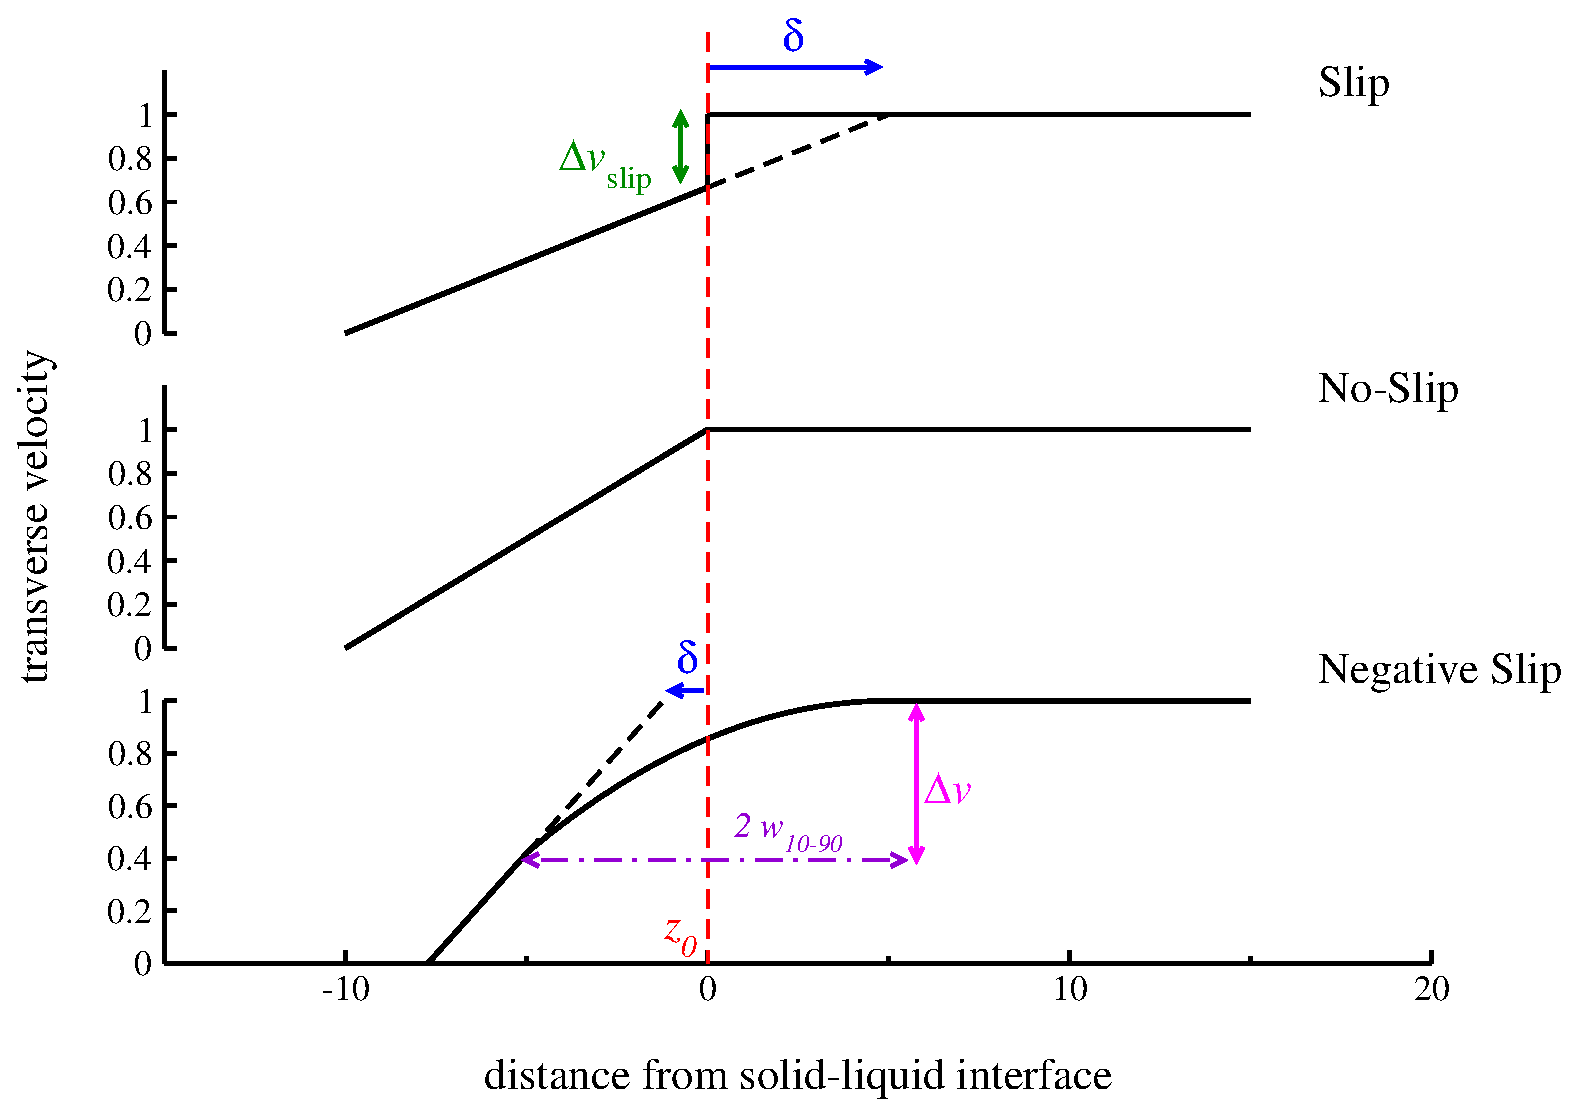
\includegraphics[width=\linewidth]{Figures/slipLengthPlot}
\caption{\label{fig:slipLength} A sketch of transverse velocity
  profiles, $v_x(z)$, for interfaces in slip (top), no-slip (middle),
  and negative slip boundary conditions (bottom).  The location of the
  interface is defined by a Gibbs dividing surface at $z_0$. Under
  negative slip conditions, the $10\%-90\%$ interfacial width,
  $w_{10-90}$, provides locations that are unambiguously on the liquid
  and solid sides of the interface.\label{fig:slipLengthPlot}}
\end{figure*}


In our initial investigation of friction at the basal and prismatic
interfaces,\cite{Louden2013a} we related the interfacial friction
coefficient to the imposed momentum flux $j_z(p_x)$ and the transverse
flow velocity gradient through a linear constitutive relation.
\begin{equation}\label{eq:linConRel}
j_{z}(p_{x})=-\eta \left(\frac{\partial v_{x}}{\partial z}\right)
\end{equation}
Substituting Equation \eqref{eq:linConRel} into Equation \eqref{eq:kappa1} gives
an expression for the friction coefficient in terms of the momentum
flux and the resulting velocity gradient through the liquid region of
the simulation box.
\begin{equation}\label{eq:lambda}
\lambda=-\frac{j_{z}(p_{x})} {\delta\left(\frac{\partial v_{x}}{\partial
      z}\right) }
\end{equation}

For ice-I$_\mathrm{h}$ / water interfaces, the boundary conditions are
no-slip, so projecting the bulk liquid state velocity profile yields a
negative slip length. This length is the difference between the
structural edge of the ice (determined by the tetrahedrality profile)
and the location where the projected velocity of the bulk liquid
intersects the solid phase velocity (see Figure
\ref{fig:delta_example} for a diagram of no-slip conditions at
ice-I$_\mathrm{h}$ / water interfaces). The coefficients of friction
for the basal and prismatic facets were determined for shearing along
both the $x$ and $y$ axes, and are given in Table
\ref{tab:lambda}. The computed friction coefficients were found to be
invariant to shear direction, as $\lambda$ was found to be within
error bars when comparing shearing in either the $x$ or $y$
dimensions. Also we observed that the basal face had about a factor of
two larger friction coefficient as compared to the prismatic
face. Lastly, we note that the computed friction coefficients were
robust under varying shear rates.

\begin{figure*}
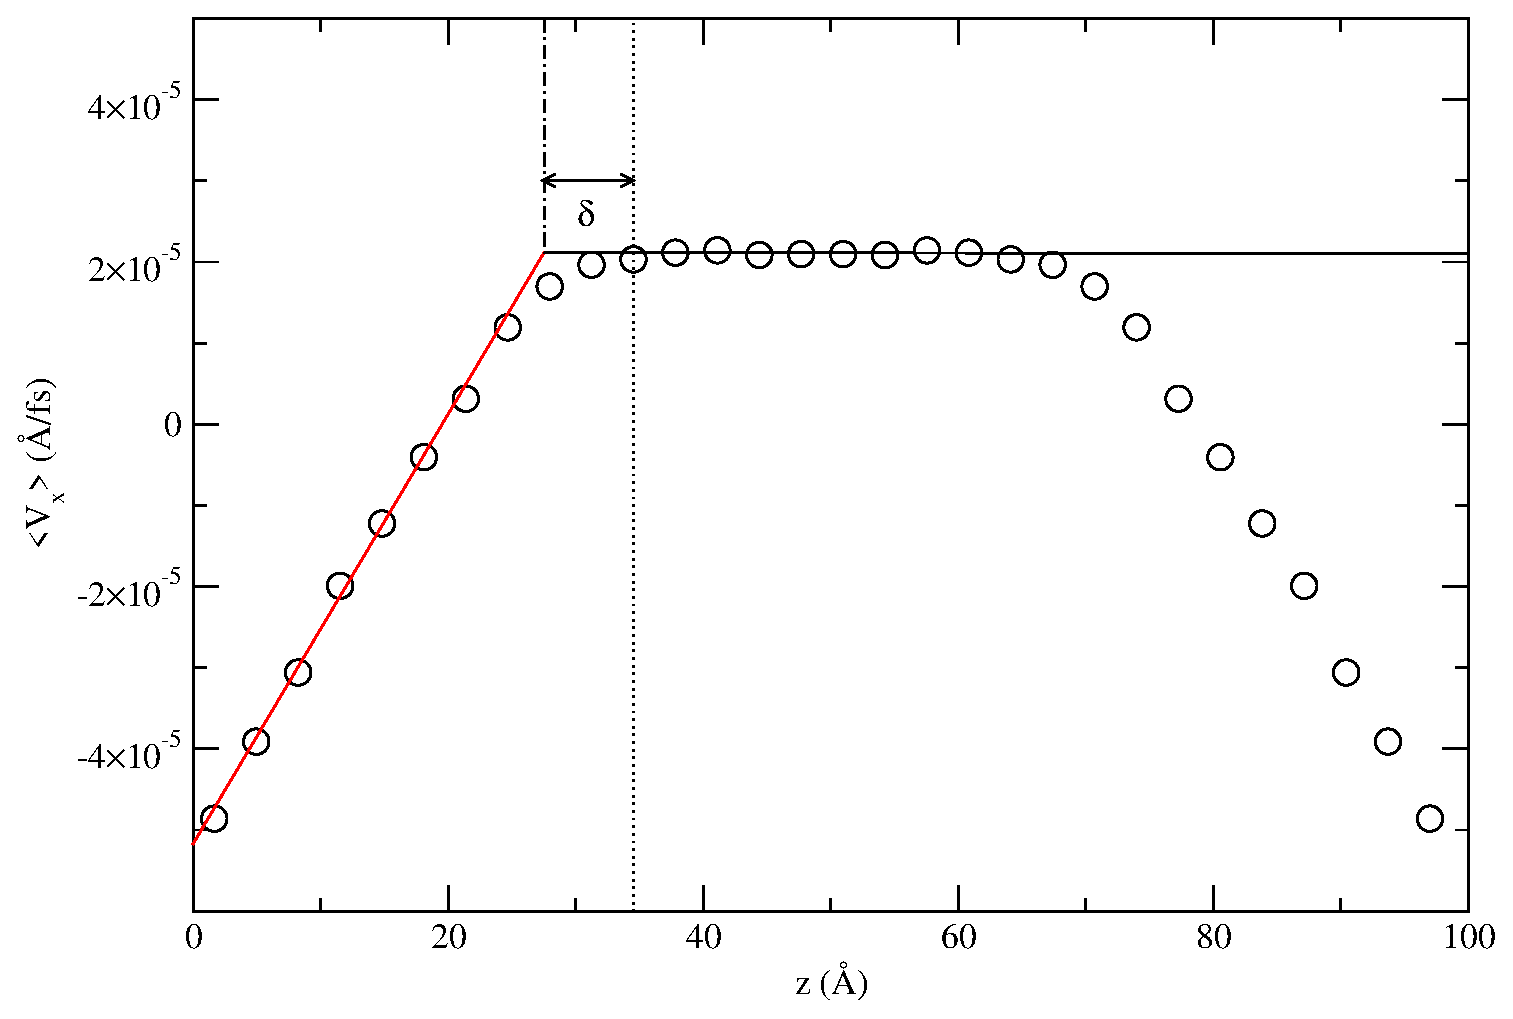
\includegraphics[width=\linewidth]{Figures/delta_example}
\caption{\label{fig:delta_example} Determining the (negative) slip
  length ($\delta$) for the ice-I$_\mathrm{h}$ / water interfaces
  (which have decidedly non-slip behavior).  This length is the
  difference between the structural edge of the ice (determined by the
  tetrahedrality profile) and the location where the projected
  velocity of the bulk liquid (dashed red line) intersects the solid
  phase velocity (solid black line).  The dotted line indicates the
  location of the ice as determined by the tetrahedrality profile.
  This example is taken from the basal-face simulation with an applied
  shear rate of 3.0 ms\textsuperscript{-1}.}
\end{figure*}

\begin{table}[h]
\centering
\caption{SOLID-LIQUID FRICTION COEFFICIENTS ($\lambda$) FOR SPC/E
  ICE-I$_\mathrm{h}$ INTERFACES WITH WATER }
\label{tab:lambda}
\begin{tabular}{r|cc}  
\hline
\hline
           & \multicolumn{2}{c}{Drag direction} \\ 
 Interface & $x$               & $y$  \\ \hline
     Basal  $\{0001\}$ &  $0.08 \pm 0.02$  & $0.09 \pm 0.03$ \\
 Prismatic  $\{10\bar{1}0\}$ & $0.037 \pm 0.008$ & $0.04 \pm 0.01$ \\ 
\hline
\hline
\end{tabular}
\begin{flushleft}
  Friction coefficients are measured in
  amu~\AA\textsuperscript{-2}~fs\textsuperscript{-1}.
\end{flushleft}
\end{table}



While this initial investigation provided some insight to friction at
ice-I$_\mathrm{h}$ / water interfaces, stick boundaries pose a problem
for Equation  \eqref{eq:kappa1}, as $\lambda$ asymptotically goes to
infinity as $\delta \rightarrow 0$.  Likewise, some materials (such as
ice-I$_\mathrm{h}$) possess solid / liquid interactions that are
strong enough for the extrapolated tangential velocity to vanish
\textit{before} reaching the solid. The velocity profile yields a
negative slip length as explained above, (bottom panel of Figure
\ref{fig:slipLengthPlot}), and the solid / liquid friction coefficient
defined in Equation \eqref{eq:kappa1} becomes meaningless.  As apparent in
Figure \ref{fig:delta_example}, the tangential velocity profile of the
liquid extrapolates to the solid velocity several molecular layers
before reaching the solid. Thus a new friction coefficient must be
defined to describe these interfaces.

A solid / liquid friction coefficient appropriate for stick
boundaries, $\kappa$, may be defined using the velocity drop
across the interface, rather than the length scale over which this
drop occurs. We can relate the imposed shear stress with the relative
tangential velocity of the fluid in the interfacial
region,\cite{Kuang2012}
\begin{equation}\label{eq:Shenyu-13}
j_{z}(p_{x}) = \kappa_{x} \Delta v
\end{equation}
where $\Delta v = v_{x}(\mathrm{solid}) - v_{x}(\mathrm{liquid})$ is
the difference in transverse velocity between points that are
unambiguously on the solid and liquid sides of the interface.  In slip
boundary conditions, $\kappa$ and $\lambda$ are identical, but
Equation \eqref{eq:Shenyu-13} provides a direct analogy to non-equilibrium
expressions for the interfacial thermal conductance $(G)$,
\begin{equation}
J_z = G~ \Delta T.
\end{equation}
Here, $J_z$ is a thermal flux and the temperature drop is measured
across an interface of \textit{finite width}. By analogy, $\kappa$ is
a transport coefficient that measures \textit{interfacial momentum
  conductance} across an interface of finite width.

At ice-I$_\mathrm{h}$ / water interfaces, the solid / liquid boundary
is not an infinitely thin plane. As we found in Chapters
\ref{chap:Str} and \ref{chap:Dyn}, a large number of order parameters
transition smoothly between the phases over a few molecular
diameters.  Here, we have used the local tetrahedral order parameter
as the metric for quantifying interfacial width and define locations
in space that are unambiguously on the solid and liquid sides of the
interface. This parameter was chosen due to its ability to
descriminate liquid-like and ice-like water molecules more accurately
than the local density, and the computed error bars were significantly
smaller than any of the dynamic order parameters investigated in
Chapter \ref{chap:Dyn}. In what follows, we have used the Gibbs
dividing surface ($z_0$) and the $10\%-90\%$ width of the interface
($w_\mathrm{10-90}^{q}$) to arrive at physical locations for measuring
$v_{x}(\mathrm{solid})$ and $v_{x}(\mathrm{liquid})$.  These uniquely
define a friction coefficient in terms of well-defined structural
features ($z_0$ and $w_\mathrm{10-90}^{q}$) and dynamic properties
($v_{x}(z)$) of the interface.

Tangential velocity profiles from the simulations were fit using a
piecewise function that is both continuous and continuously
differentiable. The velocity profiles, $v_x(z)$, obtained from each
shearing simulation were fit assuming linear behavior through each of
the three regions of the simulation box; the lower liquid, the solid,
and the upper liquid. Parabolic functions were designed to capture the
negative slip behavior that links the three regions,
\begin{equation}\label{eq:vfit}
v(z) =
\begin{cases}
  v_{l} - m_{l}z & 0 \leq z < (z_{1} - w) \\
  v_{s} - \frac{1}{2}k(z-z_{1})^{2} & (z_{1}-w) \leq z < z_{1} \\
  v_{s}  & z_{1} \leq z < z_{2} \\
  v_{s} - \frac{1}{2}k(z-z_{2})^{2}  & z_{2} \leq z <( z_{2} + w)\\
  v_{s} - \frac{1}{2}kw^{2} - m_{l}(z-(z_{2} + w)) & (z_{2} + w) \leq z \\
\end{cases}
\end{equation}
  
Here, $v_{l}$ is the velocity of the liquid at the middle of the
liquid domain (the edge of the simulation box), and $v_{s}$ is the
velocity of the solid. The locations $z_{1}$ and $z_{2}$ are the edges
of the ice slab, and $w$ is the width of the interface from the
velocity profile (distinct from $w_{10-90}^{q}$). The parameter
$m_{l}$ is the slope of the velocity profile in the liquid regions of
the box which is related to the liquid-state viscosity. Figure
\ref{fig:spComic} shows a representative velocity profile (navy
squares) and fit (green line) with the locations of $z_{1}$ and
$z_{2}$ indicated as vertical dotted lines. Once the fits were
obtained, the values for $v_{x}(\mathrm{solid})$ and
$v_{x}(\mathrm{liquid})$ for Equation \eqref{eq:Shenyu-13} were
sampled from the fit. The $z$ locations used to sample the fit were
determined by structural measures. The $z$ location for
$v_{x}(\mathrm{liquid})$ was taken to be the Gibbs dividing surface of
the interface, less the $10\%-90\%$ width of the interface. Similarly,
the $z$ location for $v_{x}(\mathrm{solid})$ was taken to be the Gibbs
dividing surface plus the $10\%-90\%$ width of the interface.

\begin{align}
v_{x}(\mathrm{solid}) & = v_{x}( z_0 + w_\mathrm{10-90}^{q})  \label{eq:vx1}\\
v_{x}(\mathrm{liquid}) & = v_{x}( z_0 - w_\mathrm{10-90}^{q}). \label{eq:vx2}
\end{align}
As mentioned earlier, the momentum flux, $j_{z}(p_{x})$ is an imposed
parameter of the VSS-RNEMD simulations, and by using
Equation \eqref{eq:Shenyu-13}, estimates of interfacial friction
coefficient $\kappa$ are straightforward.

The calculated $\kappa$ values found for the four crystalline facets
of ice-I$_\mathrm{h}$ investigated here are shown in Table
\ref{tab:kappa}. Solid / liquid friction coefficients for shearing
simulations where the imposed momentum flux was in the $y$-dimension,
$\kappa_{y}$, are calculated in the same manner, with $j_{z}(p_{y})$
and $v_{y}$ substituting for $j_{z}(p_{x})$ and $v_{x}$ in
Equations \eqref{eq:Shenyu-13}, \eqref{eq:vx1}, and \eqref{eq:vx2}.
Similar to our initial results for $\lambda$, these results
for $\kappa$ were found to be independent of the shear rate (see
Figure \ref{fig:kappaPlot}), as well as the direction of the shear
relative to the features on the surfaces of the facets.


\begin{figure*}
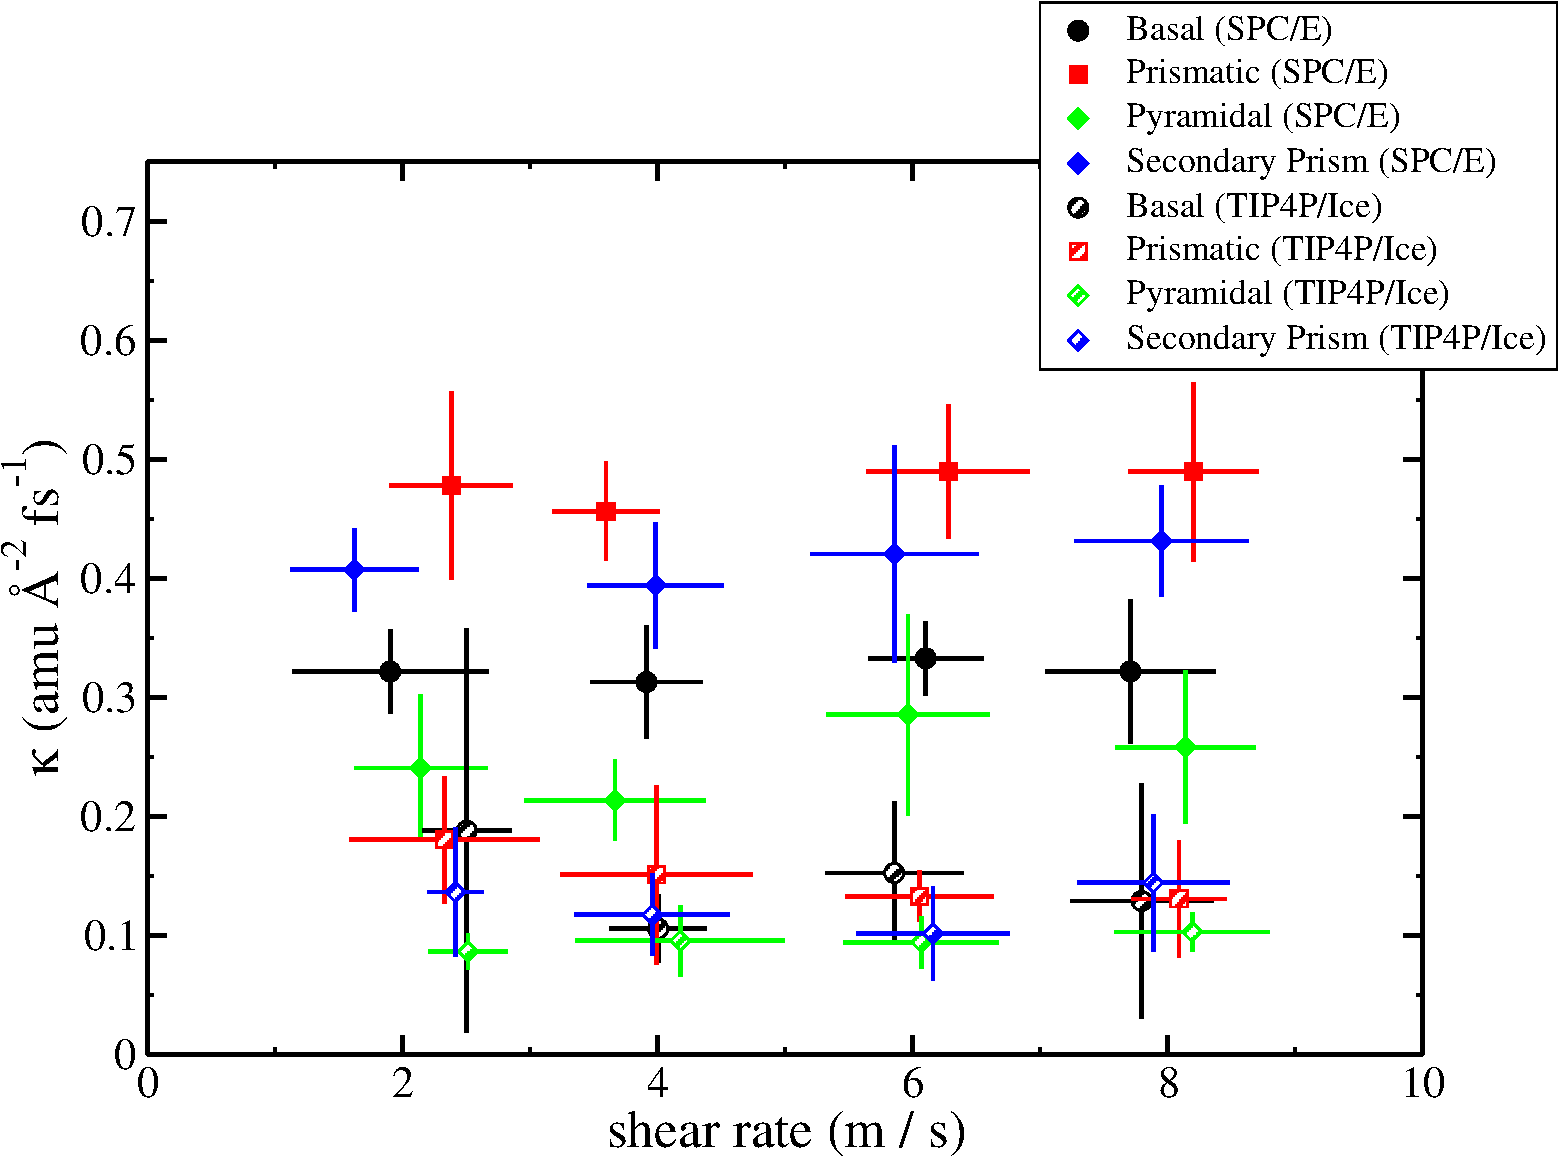
\includegraphics[width=\linewidth]{Figures/kappaPlot2}
\caption{\label{fig:kappaPlot} Dependence on the observed friction
  coefficient $\kappa$ on the shear rate of the ice through the surrounding
  liquid water.  The RNEMD simulations impose a momentum flux, but the
  resulting shear rates can vary.  Here, we collect data in 2 m/s bins
  to accumulate statistics over multiple independent simulations.  The
  SPC/E simulations (solid symbols) were done at 225~K, and the
  TIP4P/Ice simulations (patterned symbols) were carried out at
  270~K. The points on this plot have also been averaged over shear
  direction ($x$ and $y$).}
\end{figure*}


\begin{table}[h]
\centering
\caption{SOLID / LIQUID FRICTION COEFFICIENTS ($\kappa$) FOR
  ICE-I$_\mathrm{h}$ INTERFACES WITH WATER \label{tab:kappa}}
\begin{tabular}{r|cc|cc}  
  \hline
\hline
  & \multicolumn{2}{c|}{SPC/E (225~K)} & \multicolumn{2}{c}{TIP4P/Ice (270~K)} \\
  Interface & $\kappa_{x}$ &  $\kappa_{y}$ & $\kappa_{x}$ &  $\kappa_{y}$ \\ 
  \hline
  Basal  $\{0001\}$                 & 0.32(5)  & 0.31(4) & 0.12(2)  & 0.13(2) \\
  Prismatic  $\{10\bar{1}0\}$       & 0.44(5)  & 0.46(5) & 0.16(2)  & 0.16(3) \\
  Pyramidal  $\{20\bar{2}1\}$       & 0.28(3)  & 0.25(3) & 0.09(1)  & 0.10(1) \\
  Secondary Prism  $\{11\bar{2}0\}$ & 0.44(4)  & 0.42(5) & 0.14(3)  & 0.14(2) \\ 
  \hline
\hline
\end{tabular}
\begin{flushleft}
  Friction coefficients $\kappa$ are measured in amu
  \AA\textsuperscript{-2} fs\textsuperscript{-1}, and uncertainties in
  the last digit are indicated with parentheses.
\end{flushleft}
\end{table}

Note that the values of $\kappa$ for the basal and prismatic crystal
facets in Table \ref{tab:kappa} disagree with values for interfacial
friction ($\lambda$) we previously computed in Table
\ref{tab:lambda}. In our preliminary investigation, the expression for
the coefficient of friction was derived from Equation
\eqref{eq:kappa1} and the linear constitutive relation for shear
stress in a bulk fluid.  However, as described above, sheared ice /
water interfaces are in the domain negative slip lengths. Equation
\eqref{eq:kappa1} should only be used in slip boundary conditions, as
negative slip can yield coefficients of friction that appear to be
smaller in magnitude than the zero slip conditions. In our previous
work, the prismatic surface was found to have a larger negative slip
length than the basal face, indicating a prismatic surface that should
have been reported with a larger coefficient of friction. If one
instead uses Equation \eqref{eq:Shenyu-13} and interfacial widths to
compute friction, the reported values come into agreement.

The two water models give two significantly different values for the
friction coefficients. This is primarily a result of the difference in
water viscosities at the two coexistence temperatures ($\eta = $ 15.9
cP for SPC/E at 225~K and 6.1 cP for TIP4P/Ice at 270~K), which alters
the stream velocity on the liquid side of the interface. The relative
ratios of facet friction are similar in both models, however, with
$\kappa_\mathrm{prismatic} / \kappa_\mathrm{basal} =$ 1.56~(SPC/E) and
1.32~(TIP4P/Ice),
$\kappa_\mathrm{pyramidal} / \kappa_\mathrm{basal} =$ 0.84~(SPC/E) and
0.81~(TIP4P/Ice), and
$\kappa_\mathrm{secondary} / \kappa_\mathrm{basal} =$ 1.33~(SPC/E) and
1.15 (TIP4P/Ice). The observed ordering of facet friction
coefficients,
\begin{equation}
\kappa_\mathrm{pyramidal} < \kappa_\mathrm{basal} <
\kappa_\mathrm{secondary} < \kappa_\mathrm{prismatic} 
\end{equation} 
seems robust.

 
\section{Influences on Interfacial Friction}
The primary result presented in this chapter is the observation that
the different facets of ice-I$_\mathrm{h}$ produce significantly
different solid / liquid interfacial friction coefficients with water
(see Table \ref{tab:kappa}).  The two prismatic surfaces displayed the
largest coefficients of friction, while the basal and pyramidal facets
exhibited significantly lower friction. This trend is robust over a
wide range of shear rates, and shear direction relative to ice surface
features. Also, while the magnitude of the solid / liquid friction
coefficients differ due to liquid viscosities, the facet trends are
exhibited by both SPC/E and TIP4P/Ice at their coexistence
temperatures.

It is surprising that the observed solid / liquid friction
coefficients do not depend on the shear direction relative to surface
features. Pfalzgraff \textit{et al.} have recently investigated
diffusion of the water molecules comprising the quasi-liquid layer
(QLL) on the vacuum exposed basal, prismatic, and pyramidal surfaces
of an ice-I$_\mathrm{h}$ crystal.\cite{Pfalzgraff2011} They observed
anisotropic diffusion on the prismatic and pyramidal surfaces at 250~K
with the NE6 model ($\sim$~40~K below the melting temperature of that
model). In two following studies, Gladich \textit{et al.}
investigated the temperature dependence of this phenomena and deduced
the mechanism of anisotropic self-diffusivity at the prismatic
ice-vapor interface.\cite{Gladich2011,Gladich2015} They observed a
transition from anisotropic to isotropic diffusion at about 260~K with
the NE6 model, and attributed the transition to a change in the
prevailing mechanism of self-diffusion. At temperatures colder than
260~K, the QLL is sparse and the diffusing molecules are strongly
influenced by the underlying geometry of the crystal. At temperatures
warmer than 260~K, the QLL is thicker and diffusion occurs at the
outer part of the QLL. These results were robust for TIP4P/2005 and
TIP5P-Ew at the same relative undercooling temperature. Since our
ice-I$_\mathrm{h}$ / water interfaces are at their respective
coexistence temperatures, the effects of the underlying ice crystal
may be masked and we might expect to recover isotropic behavior.

The differences in friction are also surprising given that densities
and molecular interactions are identical for the four interfaces and
the interfacial widths measured via both structural and dynamic
features are also quite similar (for the interfaces treated with the
same water model). There are few remaining surface properties that
could give rise to differences in solid / liquid friction of the four
facets, notably surface corrugation, hydrogen bonding density, and
hydrogen bond lifetime at the interface. In this section we
investigate the roles of these surface features.

\subsection{Solid / Liquid Hydrogen Bond Density}
The four ice surfaces may potentially have different densities of
hydrogen bonds that bridge the solid and liquid. An ice surface that
forms more hydrogen bonds with the interfacial liquid would be able to
exert significant lateral forces on the liquid layer, yielding a
larger friction coefficient. To probe this possibility, we have
investigated the density of cross hydrogen bonds between the ice and
the liquid.

Quantifying water molecules as ``ice'' or ``liquid'' at an interface
of finite width requires a local order parameter for separating the
molecules.  Conde \textit{et al.}\cite{Conde2008} (and later Gladich
\textit{et al.}\cite{Gladich2011,Gladich2015}) discriminated molecules
as either ``ice'' or ``liquid'' by a threshold value of the local
tetrahedral order parameter (the same order parameter described here
in Section \ref{sec:tetra}), denoted $q_{t}$. This threshold value was
obtained by equating the probability of incorrectly assigning a
liquid-like molecule as ice-like to the probability of incorrectly
assigning an ice-like molecule as liquid-like. Molecules with
$q < q_{t}$ were denoted as liquid-like, while those found having
$q > q_{t}$ were designated ice-like.

In a similar manner, we have chosen a threshold value of the local
tetrahedral order parameter as our partitioning criterion. Here,
$q_{t}$ is taken to be the value of the order parameter at the Gibbs
dividing surface ($q(z_0) \approx 0.84$ for SPC/E and
$q(z_0) \approx 0.85$ for TIP4P/Ice).  Note that some molecules have
strong tetrahedral ordering in the liquid phase, so this segregation
will not yield perfect division between ice and liquid phase
molecules.

To determine if a hydrogen bond has been formed between two water
molecules, we used the geometric criteria of Luzar and
Chandler.\cite{Luzar1996} We identify a hydrogen bond between two
water molecules if the distance between their oxygen sites,
$r_\mathrm{OO} < 3.5$~\AA, and the OHO bond angle,
$\theta_\mathrm{OHO} < 30^\circ$.

For each of the shearing simulations performed, a hydrogen bond
tetrahedrality matrix was constructed.  Snapshots from the shearing
trajectories were taken every $0.1$ ps, and the tetrahedrality $(q)$
value for each water molecule in the system was calculated. Hydrogen
bonds were also identified, and the tetrahedrality of the donor
$(q_{D})$ and acceptor $(q_{A})$ molecules were recorded. A
probability density of hydrogen bonds categorized by donor and
acceptor tetrahedrality, $\rho_\mathrm{HB}(q_D, q_A)$, was then
recorded.

\begin{figure*}
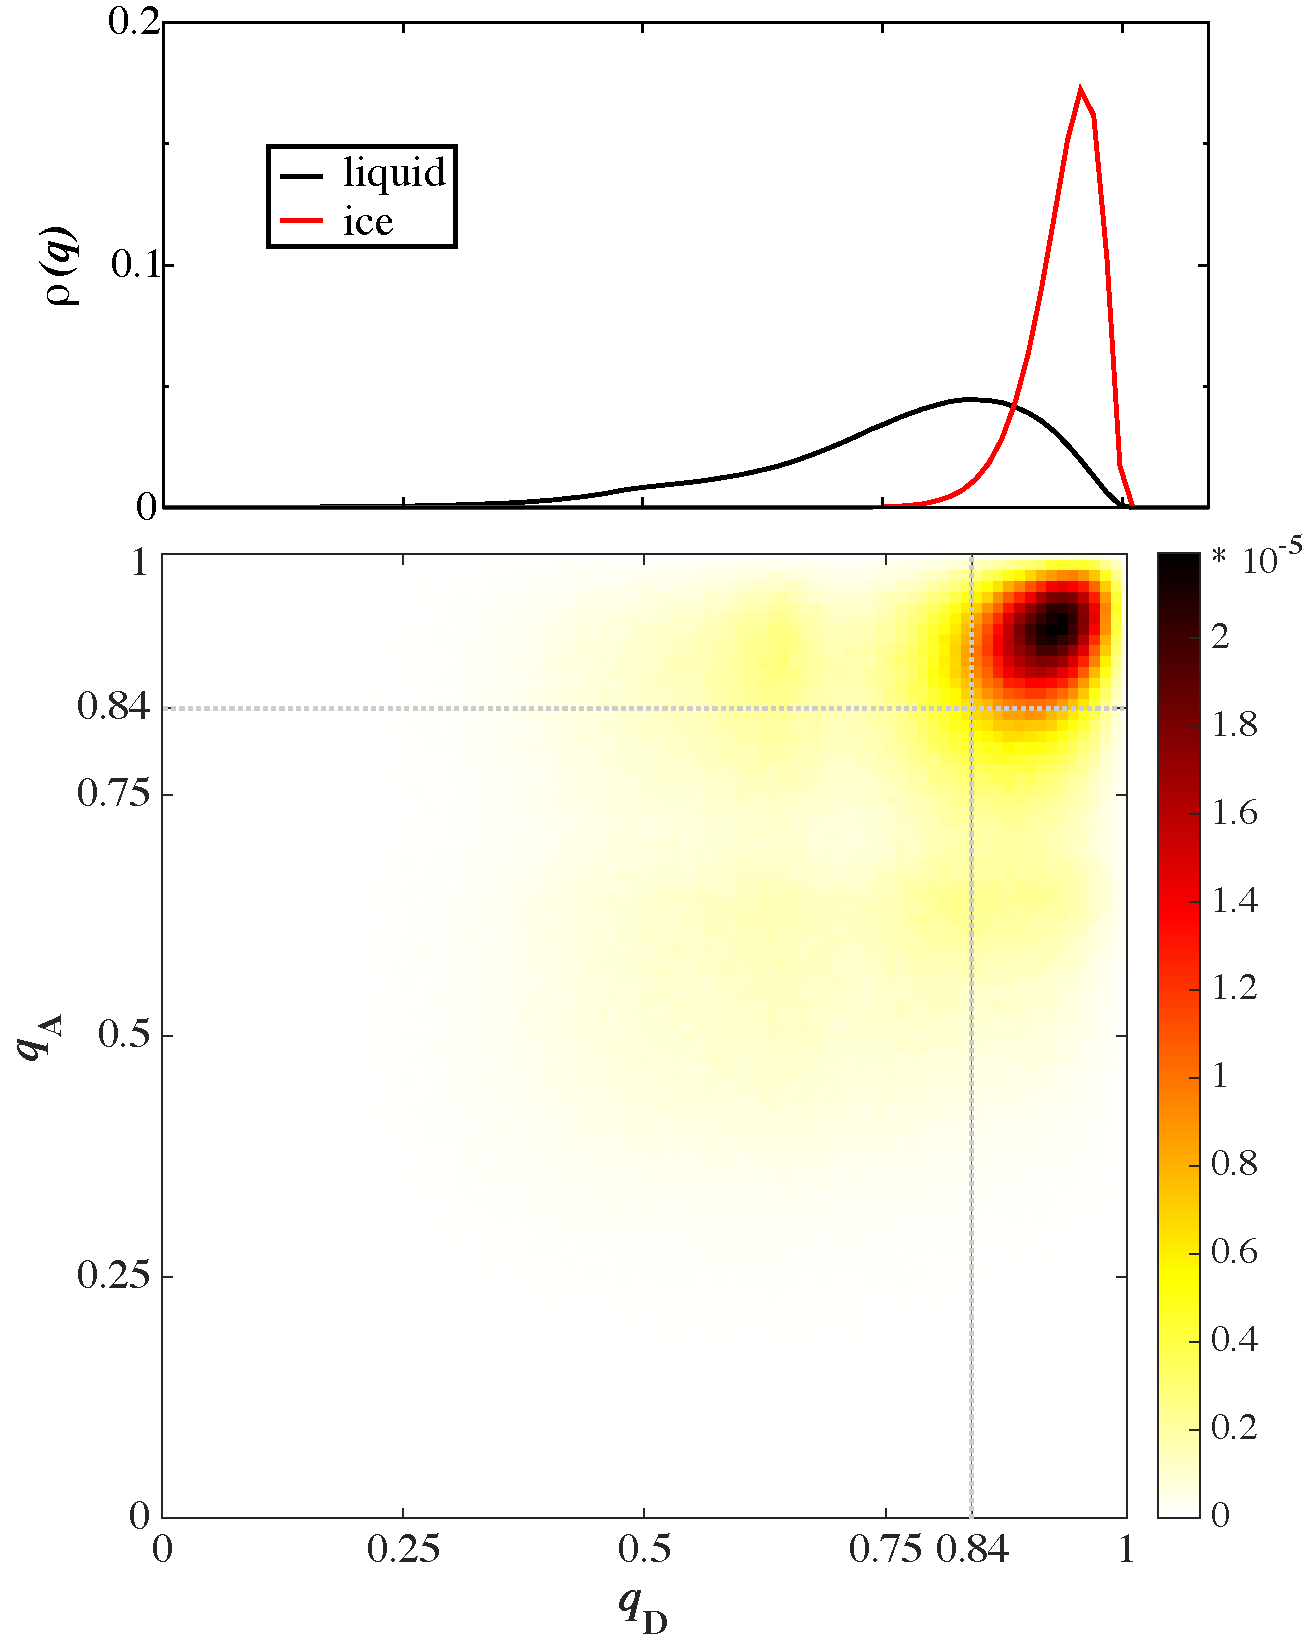
\includegraphics[width=5in]{Figures/hbtet.pdf}
\caption{\label{fig:tetHBMatrix} Distribution of hydrogen bonds at a
  prismatic interface showing the tetrahedralities of donor $(q_D)$
  and acceptor $(q_A)$ molecules (lower panel). Distributions of
  tetrahedralities in bulk ice and liquid phases are shown in the
  upper panel. The value of $q$ at the Gibbs dividing surface is
  indicated with dashed lines. Hydrogen bonds between ice molecules
  are represented by the upper right square, while those between
  liquid molecules are in the lower left.  Hydrogen bonds that bridge
  the ice-liquid interface exist primarily in the vertical and
  horizontal strips that remain.}
\end{figure*}

The lower panel of Figure \ref{fig:tetHBMatrix} shows a hydrogen bond
tetrahedrality distribution for the prismatic facet with $q_{D}$
plotted along the $x$-axis and $q_{A}$ along the $y$-axis.  Population
around $q_{D} \approx q_{A} \approx 0.9$ indicates the density of
ice-ice hydrogen bonds in the system, while the liquid-state hydrogen
bonds are concentrated in the lower left, and are significantly more
diffuse.  The off-diagonal regions of the distribution represent the
population of molecules in tetrahedral (ice-like) environments bound
to non-tetrahedral (liquid-like) environments. Integrating the
population found in each of these regions and normalizing by the
surface area of each ice crystal produces a surface density of
hydrogen bonds (\AA\textsuperscript{-2}) formed between the ice and
interfacial liquid,
\begin{equation}\label{hbondDensity}
\rho_{sl}^{\mathrm{HB}} = \frac{N_\mathrm{HB}}{2 L_{x}L_{y}} \left[ \int_0^{q_{t}}
  dq_{D} \int_{q_{t}}^1 dq_{A}~\rho_\mathrm{HB}(q_{D},q_{A}) +  \int_0^{q_{t}}
  dq_{A} \int_{q_{t}}^1 dq_{D}~\rho_\mathrm{HB}(q_{D},q_{A}) \right]
\end{equation}
$N_\mathrm{HB}$ is the total number of hydrogen bonds found in the
system, and $L_x$ and $L_y$ are the dimensions of the two ice facets
exposed to the liquid.  Values for $\rho_{sl}$ for each of the ice
surfaces are reported in Table \ref{tab:hbondDens}.

\begin{table}[h]
\centering
\caption{ SURFACE HYDROGEN BOND DENSITIES FOR SPC/E AND
  TIP4P/Ice MODELED ICE-I$_\mathrm{h}$ / WATER INTERFACES \label{tab:hbondDens}} 
\begin{tabular}{r|c|c}  
  \hline
\hline
  & \multicolumn{1}{c|}{SPC/E (225~K)} & TIP4P/Ice (270~K) \\
  Interface & $\rho_{sl}$ (\AA\textsuperscript{-2}) & $\rho_{sl}$ (\AA\textsuperscript{-2}) \\ 
  \hline
  Basal  $\{0001\}$                 & 0.1227(3) & 0.0749(9) \\
  Prismatic  $\{10\bar{1}0\}$       & 0.2014(5) &  0.141(1) \\
  14\degree~Pyramidal  $\{20\bar{2}1\}$       & 0.0866(3) & 0.074(1) \\
  Secondary Prism  $\{11\bar{2}0\}$ & 0.1384(4) & 0.119(1) \\ 
  \hline
\hline
\end{tabular}
\begin{flushleft}
Uncertainties in the last digit are indicated with
  parentheses.
\end{flushleft}
\end{table}



The trend in surface density of solid / liquid hydrogen bonds
reproduces the trend in the friction coefficients, indicating that
friction at ice-I$_\mathrm{h}$ / water interfaces is strongly influenced
by the number of solid / liquid hydrogen bonds that can be formed.
This result is robust under multiple shear rates and orientation of
shear flow relative to the surface features of the ice (that is, shear
in both the $x$ and $y$ dimensions), indicating that the hydrogen
bonding statistics between an ice facet and the liquid are not altered
by the imposed shear.

\subsection{Surface Corrugation by Projected Densities}
A second possible influence on the friction coefficient is the surface
topography of the ice crystals. To investigate this possibility, we
computed the mean projected density ($\rho(y,z)$),
\begin{equation}
\rho(y, z) = \frac{1}{L_x~dy~dz} \left< \sum_{i = 1}^{N} m_i \delta(y_i - y) \delta(z_i - z)\right>
\end{equation}
for four quiescent interfaces over 1 ns of simulation time (sampled
every 1 ps).  Here, $dy$ and $dz$ are the lengths and widths of a set of
parallelepipeds that span the box depth ($L_x$), and for relatively
small $dy$ and $dz$ (0.05 \AA), the parallelepiped densities show the
smooth transition between the ordered ice facet and the surrounding
liquid.

\begin{figure*}
\includegraphics[width=\linewidth]{Figures/DensityPlots}
\caption{\label{fig:DensPlots} Projected densities, $\rho(y, z)$, at
  the four quiescent interfaces.  Darker colors represent higher
  densities, while lighter colors (e.g. white) are relatively
  unpopulated.  For all four interfaces, the location of the
  tetrahedrality Gibbs dividing surface is indicated with a solid
  black line, while the two end points of the $10\%-90\%$ width are
  shown in grey.}
\end{figure*}

We note that the projected densities allow computation of the channel
widths and depth for the two prismatic facets using the locations of
the peak densities.  These figures also indicate that below the Gibbs
dividing surface, almost no liquid state molecules can be found
occupying the channels.  The structure of the surface corrugation can
be obtained by measuring the peak-to-peak distances of the
liquid-exposed crystal structures, the dimensions of which are
reported in Table \ref{tab:surf}. When a crystal of ice-I$_\mathrm{h}$
is cleaved along either of the two prismatic crystal facets, the
exposed oxygen atoms present channel-like structures with channel
widths of $\sim$ 5~\AA~ and channel depths of $\sim$ 2.3~\AA~.  When
cleaved along the pyramidal facet, the resulting surface features a
much larger channel, $\sim$ 8.3~\AA~ wide.  Conversely, the basal
surface presents a rather smooth surface to the liquid, with stripes
of oxygen atoms forming surface ripples with depths of $\sim$ 1~\AA~.

\begin{table}[h]
\centering
\caption{SURFACE FEATURES OF ICE-I$_\mathrm{h}$ FACETS\label{tab:surf}}
\begin{tabular}{r|cc}  
\hline
\hline
Interface & Channel width (\AA) & Channel depth (\AA) \\ 
\hline
Basal  $\{0001\}$                 & 3.5(2) & 0.9(1)  \\
Prismatic  $\{10\bar{1}0\}$       & 4.5(1) & 2.4(3)  \\
14\degree~Pyramidal  $\{20\bar{2}1\}$       & 8.3(2) & 1.9(4)  \\
Secondary Prism  $\{11\bar{2}0\}$ & 5.3(4) & 2.2(1)  \\ 
\hline
\hline
\end{tabular}
\begin{flushleft}
Uncertainties in the last digit are indicated with
  parentheses.
\end{flushleft}
\end{table}

The prismatic channels are quite stable. That is, the projected
density in the prismatic and secondary prism surface channels is small
relative to the bulk liquid density $(\rho(y,z) < \rho_l / 7)$.  One
might expect regions of low liquid density to yield smaller solid /
liquid interactions, and it does appear that these two surfaces
present roughly half of the surface oxygen atoms to the liquid.
However, the molecules forming the bottoms of the channels are fully
saturated (four hydrogen bonds each), while the molecules that form
the tops of the channels present a high density of available hydrogen
bond locations.

The oxygen-based surface features of the prism and secondary prism are
similar, and only the orientation of the water molecules varies.  This
means that the patterning of donor and acceptors on the two facets is
quite different. A liquid with internal hydrogen bonding constraints
that is in contact with these facets will allow the prismatic surface
to form a higher density of solid / liquid hydrogen bonds than the
secondary prism, even with identical oxygen ordering at the interface.

% In contrast with the prismatic facets, liquid state molecules can
% populate the surface channels on the pyramidal facet. Again, one might
% expect the interactions between the solid and the liquid in close
% physical contact to be quite large.  However, the liquid molecules
% populating this channel do not pack efficiently and cannot fully
% saturate the surface locations available for hydrogen bonding,
% resulting in a lower solid / liquid hydrogen bond density and a
% smaller coefficient of friction.

With its smooth surface, one could make reasonable physical arguments
for the basal face to have either high or low friction with liquid
water. That is, liquid molecules should be able to form a fully
populated network of hydrogen bonds with the surface, as there are no
recessed surface molecules at the bottoms of deep channels. In the
absence of large surface undulations, however, liquid-phase molecules
should also be able to slip over the surface easily. However, the
basal facet was found to have an intermediate friction coefficient
compared with the other facets studied here. The sensible explanation
in light of the hydrogen bonding data is simply that the surface
density of solid / liquid hydrogen bonds (however transitory)
dominates the interfacial friction.

\subsection{Hydrogen Bond Lifetime at the Interface}
A third possible influence to the friction at the ice-I$_\mathrm{h}$ /
water interface is that there are differential lifetimes of hydrogen
bonds for the crystal facets investigated. A crystal face with longer
persisting hydrogen bonds would impose more drag on the liquid, which
could result in a larger friction coefficient. 

In order to determine the lifetime of the hydrogen bond, we can
investigate the hydrogen bond jump rate at the interface. In Chapter
\ref{chap:Dyn} we discussed how the hydrogen bond jump rate was
calculated, and the results are presented in Figure
\ref{fig:SPCEjumpRates} and Figure \ref{fig:TIP4PIcejumpRates}. By
querying the value of $k_\mathrm{jump}^{-1}$ at each interface, we
have obtained estimates of the hydrogen bond lifetime for each of the
crystal facets under the two models. Here, we obtained $\tau_{HB}$ at
the interface as determined by both the local tetrahedral order
parameter, and as determined by the jump rates; these values are
reported in Table \ref{tab:jumpRates}.


\begin{table}[h]
\centering
\caption{HYDROGEN BOND LIFETIMES  ($\tau_{\mathrm{HB}} = k_\mathrm{jump}^{-1}$) FOR
  ICE-I$_\mathrm{h}$ / WATER INTERFACES\label{tab:jumpRates}}
\begin{tabular}{r|cc|cc}  
\hline
\hline
& \multicolumn{2}{c|}{SPC/E (225~K)}  &
                                                  \multicolumn{2}{c}{TIP4P/Ice
                                        (270~K)}  \\ 
Interface & structural & dynamic & structural
                              & dynamic \\
\hline
Basal  $\{0001\}$                 & 500 & 111 & 111 & 50 \\
Prismatic  $\{10\bar{1}0\}$       & 333 & 167 & 143 & 50 \\
14\degree~Pyramidal  $\{20\bar{2}1\}$       & 500 & 100   & 125 & 50\\
Secondary Prism  $\{11\bar{2}0\}$ & 333 &111  & 100 & 50\\ 
\hline
\hline
\end{tabular}
\begin{flushleft}
  Hydrogen bond lifetimes $\tau_{\mathrm{HB}}$ (in ps) measured at the
    structural interface (as determined by tetrahedrality) and at the
    dynamic interface (as measured by hydrogen bond jump time).
\end{flushleft}
\end{table}

We find that the lifetime of hydrogen bonds at the structural SPC/E
ice-I$_\mathrm{h}$ / water interface has a lifetime of $\sim$ 500 ps
for the basal and pyramidal facets, and about 300 ps for the two
prismatic facets. This is significantly longer than compared with the
lifetime obtained when querying at the midpoint of the hydrogen bond
jump interface, which estimates the lifetime to be about 100 ps for
each of the interfaces. Here, the prismatic surface displays a
slightly longer lifetime than the other three facets.  The TIP4P/Ice /
water interfaces have significantly shorter lived hydrogn bonds, with
lifetimes of about 100 ps at the structural interface and 50 ps at the
hydrogen bond jump interface. For all interfaces, the hydrogen bond
lifetime is observed to be longer-lived in the SPC/E interfaces as
compared to the TIP4P/Ice interfaces. This is primarily due to the
warmer coexistence temperature for the TIP4P/Ice model, leading to
faster dynamics of the water molecules. However, there is no observed
trend in the lifetime of the hydrogen bonds with the computed friction
coefficients, further indicating that friction at ice-I$_\mathrm{h}$ /
water interfaces is governed by the density of solid / liquid hydrogen
bonds, and not the dynamics of hydrogen-bond breaking / formation.

\section{A Simple Model For Solid-Liquid Friction}
The interfacial friction coefficient, $\kappa$, captures the momentum
conductance transverse to the interface, and this momentum should be
transferred via strong intermolecular interactions across the
interface. This is measured in ice-I$_\mathrm{h}$ / water systems by
the surface density of hydrogen bonds,
$\rho_\mathrm{s-l}^{\mathrm{HB}}$.  The momentum is then carried
through the liquid via viscous forces $(\eta)$ across an interfacial
region that has width $w_\mathrm{s-l}$. A simple linear model,
\begin{equation}
  \kappa = c~~\rho_\mathrm{s-l}^{\mathrm{HB}}~~\eta~~w_\mathrm{s-l},
\label{eq:model}
\end{equation}
captures these features at the ice-I$_\mathrm{h}$ / water interface,
and the results for the two water models nearly coalesce with a
proportionality constant, $c = 0.343$ (see
Figure \ref{fig:simpleModel}).  The structural width,
$w_\mathrm{10-90}^{q}$, and values for $\eta$ for each ice / water
system were obtained by fitting the liquid portions of the simulation
box in conjunction with Equation \eqref{eq:viscosity}.  The two water
models have different coexistence temperatures, so they exhibit
different hydrogen bond densities and viscosities adjacent to the
interface.  Comparing Equation \eqref{eq:model} with the non-equilibrium
expressions for $\kappa$ (Equation \eqref{eq:Shenyu-13}) and $\eta$
(Equation \eqref{eq:viscosity}) shows that the liquid's viscosity is an
important feature in capturing the velocity drop on the liquid side of
the interface ($\eta w_\mathrm{s-l}$), but the magnitude of the
solid-liquid interactions ($c~~\rho_\mathrm{s-l}^{\mathrm{HB}}$) plays a central
role in the observed friction.

\begin{figure*}
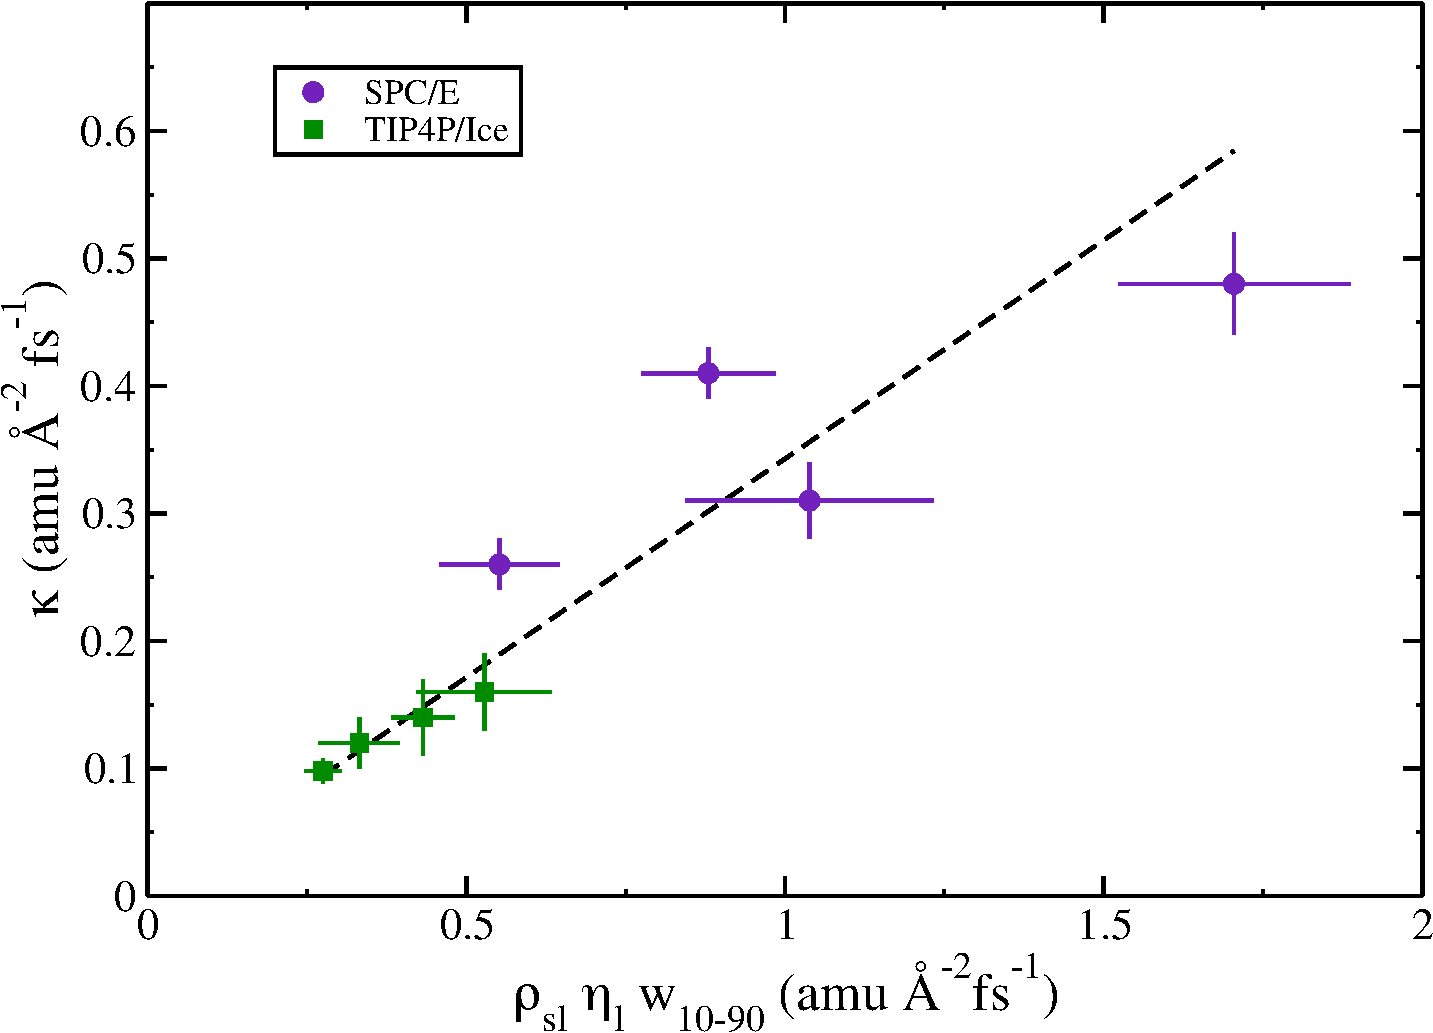
\includegraphics[width=\linewidth]{Figures/simpleModel}
\caption{\label{fig:simpleModel} Solid-liquid friction coefficients
  shown vs. surface hydrogen bond density model (Equation \eqref{eq:model})
  for all four facets and for both water models.  Although SPC/E
  (225K) and TIP4P/Ice (270K) operate in two distinct viscosity
  domains, the model captures the importance of the density of
  solid-liquid hydrogen bonds.}
\end{figure*}                                            

\section{Summary}
RNEMD simulations of the different facets of ice being drawn through
surrounding water at the coexistence temperature indicate
facet-dependence of solid / liquid friction.  We have defined a
negative slip interfacial friction coefficient, $\kappa$ (measured in
amu~\AA$^{-2}$ fs$^{-1}$) and find that the two prismatic facets exert
the largest drag on the surrounding liquid.  The basal facet provides
an intermediate level of drag, while the pyramidal facet has roughly
half the interfacial friction of the prismatic facet.

Using the local tetrahedral order parameter as a metric to
differentiate ice and liquid water molecules and a geometric hydrogen
bonding criteria, the friction coefficients were shown to be largely
governed by the surface density of solid / liquid hydrogen bonds
($\rho_{sl}^{mathrm{HB}}$).  A simple linear model, Equation
\eqref{eq:model}, uses this density to provide estimates of
solid-liquid friction that give good agrement for two different water
models at their respective coexistence temperatures.

In Chapter \ref{chap:Str} and Chapter \ref{chap:Dyn}, we presented
evidence that the ice-I$_\mathrm{h}$ / water interfacial widths for
all four crystal facets are similar (using both structural and dynamic
measures) and found these widths to be independent of shear rate.  The
similarity of interfacial width estimates for the four facets indicate
that the particular facet of the exposed ice crystal has very little
effect on how far into the bulk the ice-like structural ordering
persists. While differences have been found in previous simulations of
ice-I$_\mathrm{h}$ / water interfaces,\cite{Hayward2001,Hayward2002}
experimentally these differences have been less
clear.\cite{Beaglehole1993} The significant differential friction
coefficients obtained here suggest that while the liquid next to the
ice might be structurally organized like bulk liquid, the dynamics of
the molecules are still quite strongly perturbed by the ice.  That is,
the surface hydrogen bonding significantly alters how the water layers
are pulled along with the ice during shear.




%%%%%%%%%%%%%%%%%%%%%%%%%%%%%%%%%%%%%%%%%%%%%%%%%%%%%%%%%%%%%%%%%%%%%%%%%%%%%%%%%%%
%		CHAPTER 6 -- QLL VISCOSITY
%%%%%%%%%%%%%%%%%%%%%%%%%%%%%%%%%%%%%%%%%%%%%%%%%%%%%%%%%%%%%%%%%%%%%%%%%%%%%%%%%%%
\chapter{MEASUREMENTS OF THE VISCOSITY OF THE QUASI-LIQUID LAYER AT THE SURFACE OF ICE-I$_\mathrm{h}$}\label{chap:QLL}

\begin{flushright}
\textit{''Why do snowflakes always fall as flat structures with six corners?''} \\
-Joannes Kepler (1611) \\
\end{flushright}

In the hydrodynamic friction regeime for a slider passing over an ice surface, three distinct forces contribute to the overall observed friction; the solid-liquid friction between the ice and quasi-liquid layer (QLL), the viscous shearing of the qll, and the solid-liquid friction between the qll and the slider. In Chapter \ref{chap:Friction}, we presented facet-dependent friction coefficients for the basal, prismatic, 14\degree~pyramidal, and secondary prism ice-I$_\mathrm{h}$ / water interfaces. In this chapter, we discuss the contribution of the viscous shearing of the qll at the basal and prismatic ice-I$_\mathrm{h}$ / vapor interface.



\section{Computational Methods}
TIP4P-Ice basal and prismatic ice-I$_\mathrm{h}$ primitive crystals were constructed following the procedure described in Chapter \ref{chap:Methods}. These primitive cells were then reoriented so that the desired crystal face was exposed to the $y$ axis, then replicated in the $x$ and $z$ dimensions to form large sheets. The sheets were then replicated in $y$ until the basal crystal was 12 bilayers thick, and the prismatic cyrstal was replicated to a width of approximately equal to the basal crystal. Dimensions and number of molecules in each system are found in Table \ref{tab:qll-method}.


\begin{table}[h]
\centering
\caption{SIZES OF THE VAPOR EXPOSED ICE-I$_\mathrm{h}$ / QUASI-LIQUID LAYER SIMULATIONS\label{tab:qll-method}}
\begin{tabular}{r|c|ccc}
\hline
\hline
 Interface & $N_\mathrm{ice}$ & $L_x$ & $L_y$ & $L_z$ \\
\hline
Basal  $\{0001\}$                           & 46,080 & 185.24 & 44.04 & 186.06 \\
Prismatic  $\{10\bar{1}0\}$            & 55,000 & 192.47 & 49.14 & 181.61\\
\hline
\hline
\end{tabular}
\begin{flushleft}
Box dimensions are given in \AA.
\end{flushleft}
\end{table}


The $y$-dimension of the simulation box was then set to 300~\AA~ to allow for a surface premelt to form, and each system was equilibrated to 265~K~. The resulting systems exposed two interfaces, one toward positive $y$ and the other towards negative $y$. The equilibration was conducted under a constant pressure and temperature integrator, allowing the $x$ and $z$-dimensions of the simulation cell to relax and alleviate any crystal strain. Following this the systems were then equilibrated under a constant volume and temperature integrator, and lastly under a constant volume and energy integrator. During these simulations, the width of the crystal (in the $y$-dimension) was monitored to ensure no appreciable crystal melt occurred.

Once equilibrated, a shear stress was applied only to molecules within the QLLs using the velocity shearing and scaling variant of reverse non-equilibrium molecular dynamics described in Chapter \ref{chap:Methods}.\cite{Kuang2012} The VSS-RNEMD exchange regions were defined to incorporate molecules from both the top and bottom interfaces, as seen in Figure \ref{fig:qll-rnemd}. Both the tangential density and tetrahedrality profiles were used to determine the $y$-width of the exchange VSS-RNEMD regions. In Chapter \ref{chap:Str}, we found the tetrahedrality at the Gibbs dividing surface for ice-I$_\mathrm{h}$ / water interfaces to be $q^{Gibbs} \sim$0.84. Here, we have used $q^{Gibbs}$ as the cutoff value between the QLL and the ice. All molecules with $q < q^{Gibbs}$ are denoted as QLL molecules, while those with $q > q^{Gibbs}$ are denoted to be ice. This cutoff coincides with a minimum in the tangential density profiles, as seen in the top and bottom panels of Figure \ref{fig:qll-rhoq}.


\section{Distance Dependence of Viscosity from the Ice Surface}
As seen in Figure \ref{fig:qll-rhoq}, the QLLs at the surface of the
basal and prismatic crystals form a bilayer. Following Neshyba
\textit{et al.}, we denote the following definitions; molecules within
the ice are labeled as $\mu_{i}$, where each $i$ denotes a unique
density peak in the ice, molecules in the QLL layer closer to the ice
are labeled as $\epsilon_{2}$, and molecules in the outter portion of
the QLL bilayer are labeled as $\epsilon_{1}$.\cite{Neshyba2009} Due
to their relative distances from the underlying crystal, molecules
within layers $\epsilon_{2}$ and $\epsilon_{1}$ experience vastly
different local environments. Water molecules within $\epsilon_{2}$
located closer to the ice experience significantly more drag than
those closer to the vapor. Therefore, we expect a noticeably different
sheaer viscosity for the molecules located in $\epsilon_{2}$ and
$\epsilon_{1}$. 

The shear viscosity, $\eta$, of the QLL can be determined using the linear
constitutive relation for a shear stress imposed across a liquid.
\begin{equation}\label{eq:qll-visco}
j_z(p_x) = \eta \frac{\partial v_x}{\partial z}
\end{equation}
Since the QLLs are composed of multiple layers of varying densities
and local structures, their response to the shear stress may vary. Due
to this, we have computed $\eta$ for thin slices of $y$ through the
QLLs as seen in Figure \ref{fig:qll-vx}.

\begin{figure}
\includegraphics[width=\linewidth]{Figures/qll-vx}
\caption{\label{fig:qll-vx} Shearing profiles of the basal QLLs for
  molecules close to the underlying ice surface ($\epsilon_{2}$) and
  molecules closer to the vapor ($\epsilon_{1}$). }
\end{figure}                


\begin{figure}
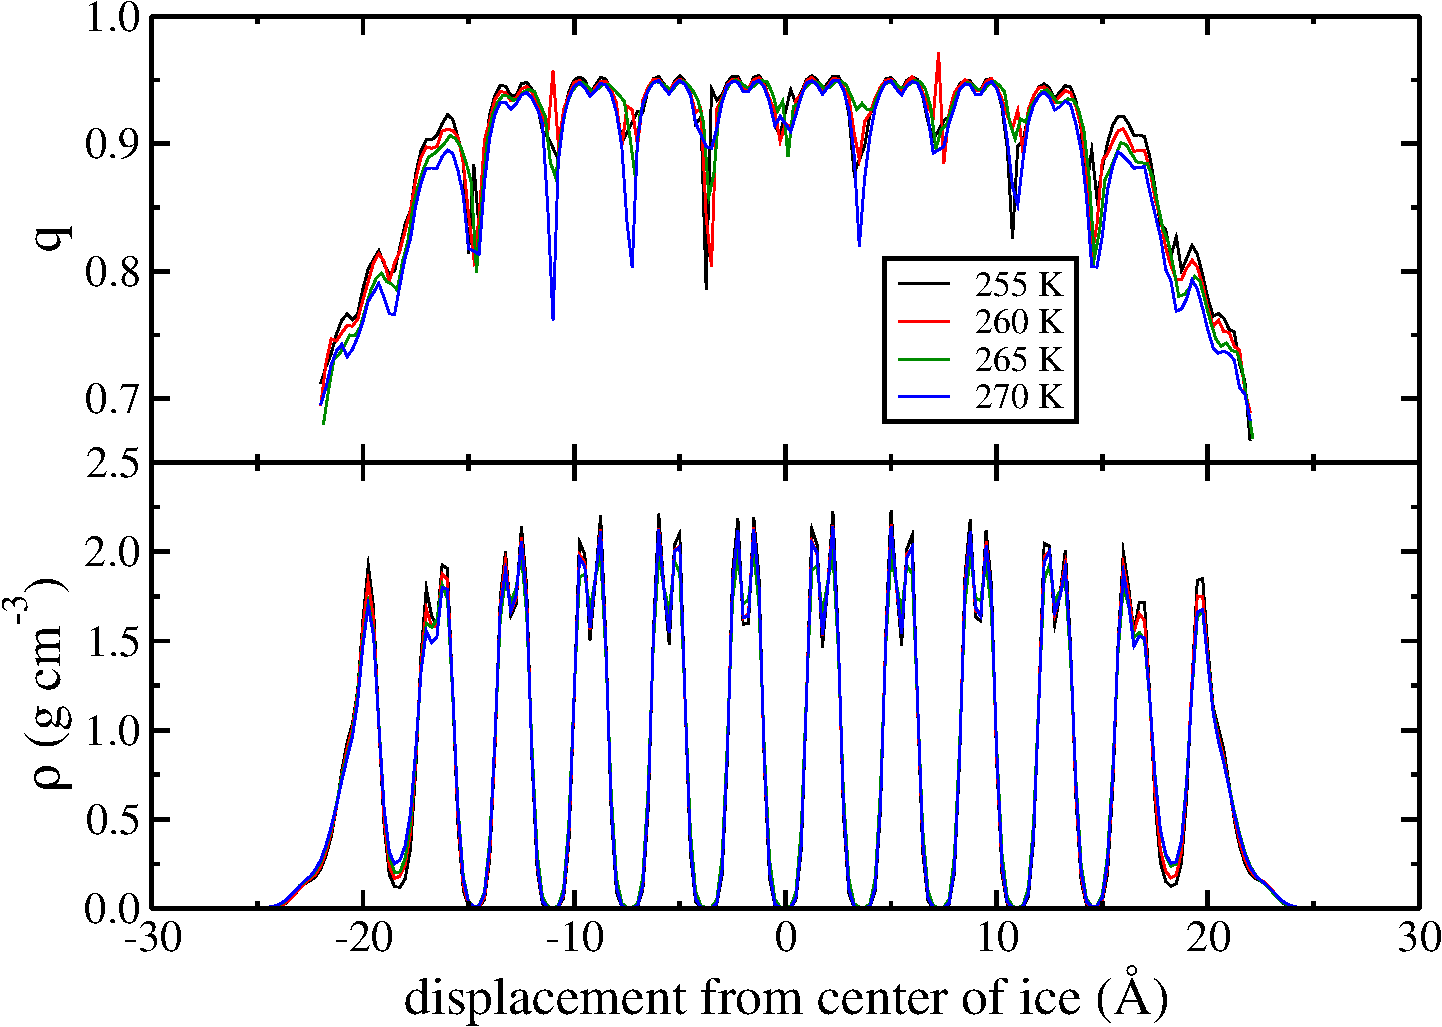
\includegraphics[width=\linewidth]{Figures/basal_rhoq}
\caption{\label{fig:basal_rhoq} Shearing profiles of the basal QLLs for
  molecules close to the underlying ice surface ($\epsilon_{2}$) and
  molecules closer to the vapor ($\epsilon_{1}$). }
\end{figure}                


\begin{figure}
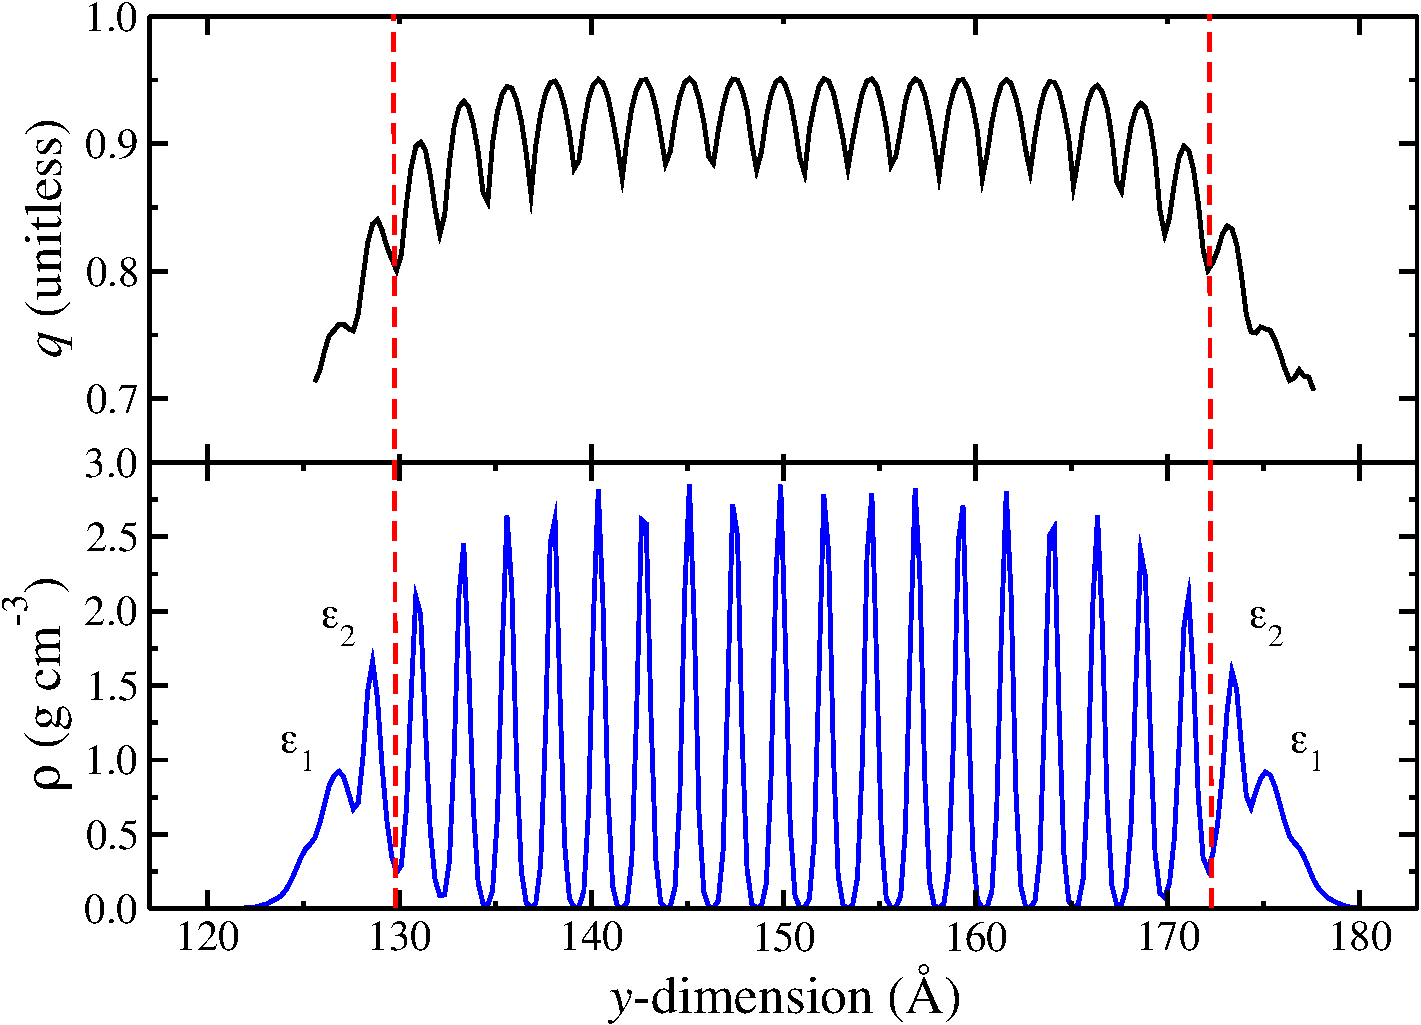
\includegraphics[width=\linewidth]{Figures/prism_rhoq}
\caption{\label{fig:prism_rhoq} Shearing profiles of the basal QLLs for
  molecules close to the underlying ice surface ($\epsilon_{2}$) and
  molecules closer to the vapor ($\epsilon_{1}$). }
\end{figure}                



Previous estimates of the viscosity of the quasi-liquid layer (QLL) on the surface of
ice have come from the Stoke's-Einstein relation, which relates the
diffusion of the surface molecules to the viscosity. However,
molecules at the surface of ice which are transitory in the vapor
phase can skew the results, as their mean-square displacements will be
much larger than those in the condensed phase. Due to this, our
estimates which are much less sensative to temporary vapor phase
trajectories, provide better computational estimates of the viscosity
of the qll.

Neshyba \textit{et al.} studied the basal qll using the six site water
model developed by Nada and van der Eerden. Neshyba investigated water
accommodation and sublimation events, focusing on the underlying
mechanisms for the events to occur. They observed long rotational and
thermal relaxation of incident gas phase water molecules as they
condensed into the qll and into the ice. \cite{Neshyba2009} 


% In a recent review of Ice Surfaces, Mary Jane Shultz posed numerous
% open questions about the qll, such as what is the growth mechanism,
% relative energies of various vaces are not well understood, what is
% the impact of face termination on ice surface energy and reactivity,
% what defintion is relevant for the qll, at what temperature does the
% qll from, what is the nature of the qll?

2017 PNAS paper by M. Alejandra Sanchez \textit{et al.} provides
experimental (surface-specific vibrational sum frequency generation
spectroscopy)  and theoretical (molecular dynamics simulations with
the TIP4P/Ice model)
evidence that the qll formation occurs
bilayer-by-bilayer. Observed for the basal face and the secondary prism. 

% Determination of Surface Tension-to-Shear VIscosity Ratio for
% Quasiliquid layers on Ice Crystal Surfaces.
%   K. Murata, H. Asakawa, K. Nagashima, Y. Furukawa, G. Sazaki
%   PRL 115 (2015) 256103
Using laser confocal microscopy in conjunction with an inverted
optical microscope, Murata \textit{et al.} have recently measured the
characteristic-velocity (\textit{i.e.} the surface tension-to-shear
viscosity ratio) of two distinct wetting morphologies of QLLs on the
basal surface of ice at -0.2 degrees Celcius and a pressure of 578.9
Pa.\cite{Murata2015} They observed a partial wetting QLL, described as
a bulk liquid droplet (BLD), as well as a complete wetting state,
described as a thin liquid layer (TLL). The characterstic-velocity of
the BLDs was determined from relaxation modes of their contact lines,
which was observed to decay with single exponential behavior according
to
\begin{equation}
u_q = u_q(0) exp\Bigg(-\frac{V^* \theta^3 q}{3l}t\Bigg)
\end{equation}
where $q$ is the wave vector for the perturbing mode for the
relaxation of the amplitude of the contact line and $u_q(0)$ being the
initial amplitude of the mode. Here, $V^* = \gamma / \eta$ is the
characteristic velocity and $\theta$ is the contact angle the BLD makes
with the ice surface ($\sim$ 2 degrees). Lastly, the logarithmic factor
$l=ln(L/a)$ is a cutoff parameter which helps avoid
singularities. From this fit, they obtained $V^* = 2 \pm 1$ m/s, which
is about an order of magnitude smaller than that of bulk water, 42.21
m/s.

Murata \textit{et al.} also investigated the spreading dynamics of the
BLD-QLLs, during the transformations to TLL-QLLs. The radii of the
spreading BLD-QLLs were fit to a power law
\begin{equation}
r = L (\frac{4S}{3Ll \eta})^{1/4}(t+t_0)^{1/4}.
\end{equation}
Here, $S$ is the spreading coefficient, and $t_0$ captures the initial
state of the droplet. As the QLL transitions from the BLD
drpolet-shape to the TLL pancake-shape, the volume must be
conserved. From this conservation, Murata \textit{et al.} estimated
the thickness of the TLLs as 9 $\pm$ 3 nm.

Lastly, Murata \textit{et al.} have obtained the characterstic
velocity of the TLLs in the same way as the BLDs. However, here the
hydrodynamic dissipation is not located at the wedge of the droplet
like in the BLD case, but instead the dissipation occurs within the
fluid of the pancake-shape object itself. Due to this, a slightly
different expression for the viscious force must be used, and the
resulting characteristic velocity was found to be $V^* = 0.2 \pm 0.1$
m/s, about 200 times smaller than that of bulk water. This seems to
imply a dependence on the characterstic velocity to the QLLs contact
area and distance from the surface. The BLD droplet-shaped QLLs (where
the QLL is only partially wets the surface and a larger amount of the
QLL resides further from the surface), were found to have a
characterstic velocity of about an order of magnitude larger than the
more completely wetting state, where more of the QLL resides closer to
the surface.

It is interesting to note that the surface tension of the BLD/air
interface ($\gamma_t$) is approximately equal to the TLL/air interface
surface tension ($\gamma_b$), as there is observed coexistence of both
forms of QLLs at the same time. Therefore, the discrepency in $V^*$
can be primarily attributed to the shear viscosity of the QLL phase.
 
% end Murata2015


Discuss widths of qll by experimental groups. Probing different
measures of the qll gives different widths at different
temperatures. Give a quick summary of the kinds of experiments and
what their findings were for qll widths.




Break down of stoke's-einstein relation for viscosity. \cite{Chen2006,
  Tarjus1995,Bordat2003,Kumar2007}


% The thickness of a liquid layer on the free surface of ice as
% obtained from computer simulation. M.M.Conde, C.Vega, A.Patrykiejew
% JCP 129, 014702 (2008)
%Outstanding references and background
Molecular dynamics simulations of ice-I$_\mathrm{h}$ with a free
surface were performed using the SPC/E, TIP4P, TIP4P/Ice, and
TIP5P/2005 water models. The basal, prismatic, and secondary prismatic
surfaces exposed to vacuum were analyzed. Conde \textit{et al.}
observed that the thickness of the liquid like layer that develops on
the surface of the ice is of approximate thickness for a given plane
across all water models, when comparison is made at the same relative
undercooling temperature for the water models.\cite{Conde2008} In all
cases the width of the liquid layer is found to increase with
increasing temperature. For a given temperature, the following trend
in QLL thickness was observed, the basal plane > the primary prismatic
plane > the secondary prismatic plane. For the TIP4P/Ice model, the
onset temperature of the QLL was observed at -100 degrees Celcius for
the basal plan, -80 degrees Celcius for the primary prismatic plane,
and -70 degrees Celcius for the secondary prismatic plane. NVT
simulations between 6 and 12 ns. To discriminate icelike and
liquidlike water molecules, they have used the local tetrahedral order
parameter of Errington and Debenedetti. However, their values are
locked at only the four closest neighbors.

Conde \textit{et al.} have computed probability densities of the local
tetrahedral order parameter, $p(q)$, for both a bulk liquid and bulk
icesystem for all the models investigated. The TIP4P model results
were almost indistinguishable, and the SPC/E model results were in
good agreement with the TIP4P/Ice results considering the large
discrepency between the melting points of the models. However, there
is visible overlap between the bulk liquid and bulk ice distributions,
making discrimination between icelike and liquidlike molecules
difficult. Therefore, they defined a cutoff value of $q$, denoted
$q_{t}$, where molecules with $q < q_t$ are denoted to be liquid-like,
and molecules found with $q > q_t$ are denoted as ice-like. 
\begin{equation}
\int_{q_t}^{1} p_{liquid}(q)dq = \int_{0}^{q_t} p_{I_h}(q)dq
\end{equation}
Here, $\int_{q_t}^{1} p_{liquid}(q)dq$ is the probability of
incorrectly assigning a liquidlike water molecule as icelike, and
similarly $\int_{0}^{q_t} p_{I_h}(q)dq$ is the probability of
incorrectly assigning an icelike water molecule as
liquidlike. Graphically, $q_t$ is the value of $q$ where the area
under the $p_{liquid}(q)$ curve to the left of $q_t$ is equal to the
area under the $p_{I_h}(q)$ curve to the right of $q_t$.  The values
for $q_t$ were found to be approximately the same for each model
investigated, with $q_t$ (SPC/E) $\sim 0.9101$ and
$q_t$ (TIP4P/Ice) $\sim 0.9076$. 

The width of the QLL was obtained by
\begin{equation}
\delta =
\frac{N_\mathrm{liquid}M}{2\rho N_\mathrm{AV}L_\mathrm{y}L_\mathrm{z}}
\end{equation}
where $N_{liquid}$ is taken to be the average number of liquid-like
molecules during the simulation, $M$ is the molecular weight of water,
$N_{AV}$ is Avagadro's number, the product $L_yL_z$ is the area of the
exposed crystal face, and $\rho$ is the density of liquid water. The
factor of 2 in the denominator accounts for the two interfaces which
are presented by the crystal in the simulation cell. However, their
definition of the thickness of the QLL is inherently flawed in the
following way. Since their definition of liquid-like molecules comes
from their local tetrahedral order number which assumes four nearest
neighbors, molecules at the surface of the crystal will have an
artificially low value for $q$ and be labled as liquid-like, even
though their structure (based on angles between neighbors) is
indicitive of an icelike environment. A rescaling based on the number
of neighbors present would give a more accurate result. 

Conde \textit{et al.} also considered a dynamic criteria for whether a
water molecule is liquidlike or icelike. They computed the mean-square
displacement of each water molecule, and compared these values to
reference data of the TIP4P/2005 water model mean-square displacement
of bulk ice and bulk liquid water simulations. They quantified an
icelike molecule to have a mean-square displacement of less than 1
\AA~ after 400ps, and classified molecules as liquidlike if their
mean-square displacement was greater than 1 \AA~ otherwise. While the
structural and dynamic widths are not precisely the same, they are on
the same order of magnitude, similar to our own results. 
%end Conde2008


%Anisotropy in structural phase transitions at ice surfaces: a
%molecular dynamics stdy. H. Nada and Y. Furukawa, 1997, Applied
%Surface Science, 121/122, 445-447. Nada1997
720 water molecules in each ice slab, exposing the basal and prismatic
surfaces. basal system was (22.4 x 23.3 x 43.8) \AA and the prismatic
system was (22.4 x 21.9 x 46.6) \AA. The TIP4P water model was
used. Simulations were performed between temperatures of 220 and 250
K, in incrementes of 5 K. NVT simulations performed. To estimate the
thickness of the quasi-liquid layer, root mean square fluctuations in
the oxygen-oxygen length between molecules was calculated for bins of
molecules normal to the interface.
\begin{equation}\label{eqNada1997-1}
\delta = \frac{2}{n(n-1)} \sum_{i<j}^{n}
\frac{\sqrt{<r_{ij}^{2}>-<r_{ij}>^{2}}}{<r_{ij}>}
\end{equation}
Here, $n$ denotes the number of water molecules, $r_{ij}$ the distance
between oxygen atoms of water molecules $i$ and $j$ respectively, and
the angle brackets denote a times average. For a slice of molecules
with a $\delta \ge 0.1$, they are denoted as satisfying the criteria
to be a quasi liquid layer. This criteria is known as the Linemann
criterion (ref. 11 therein). Nada and Furukawa estimated the width of
the QLL to be about 11.5 \AA for the basal ice/vapor interface, and 9
\AA for the prismatic interface, respectively. They also observe
increasing QLL thickness with increasing temperature. Also, for low
temperatures, they observed the prismatic surface having a thicker
QLL, while at higher temperatures, the basal QLL was predicted to be
thicker, with the transition occurring around 235~K. \cite{Nada1997}
%end Nada1997

% Anisotropic Surface Melting of an Ice Crystal and its Relationship
% to Growth Forms. Y. Furukawa and H. Nada. J. Phys. Chem. B 1997,
% 101, 6167-6170.
Experiments have shown that anisotropic surface mleting occurs on the
surface of the basal and prismatic faces of an ice crystal, just below
the melting point. That is, at temperatures approaching the melting
point, the basal QLL is thicker than the prismatic QLL. 

A nice summary of ellipsometry measurements is given in the
intro. References 12 and 14 therein, simultaneously measured both the
thickness of the QLL as well as the index of refraction of the
transition layer on the ice surface using null elipsometry (what is
null elipsometry). From -2 degrees Celcius, the thickness of the QLL
steeply increased with increasing temperature. The index of refraction
was found to be 1.330 (which converts to a density of 991
$kg/m^{3}$. Comparitively, the index of refraction for water is 1.333
and bulk ice is 1.308. The QLL thickness of the prismatic facet was
found to be proportional to $delta T ^{-1/3}$ above -2 degrees
celcius, while the basal temperature dependence was much steeper. They
also observed a flat facet at the melting point for the basal face,
however, the prismatic facet exhibited a rounded surface at -2C. Thus
a roughening transition is beleived to occur on the prismatic facet
while not on the basal facet.\cite{Furukawa1997} 

Current work, TIP4P water model for 720 water molecules. At 250~K, the
basal face has a thinner QLL than the prismatic. This turns over at
260~K where they are approximately equal width, and at warmer
temperatures the basal is observed to have a thicker QLL. Furukawa and
Nada used the $S$ order parameter of Karim and Haymet which depends on
the orientational ordering of neighboring molecules.\cite{Karim1988}
This parameter is unity for an ordered arrangement of water molecules
in an ice crystal, and $\approx$ 0.3 for a random
arrangement. Furukawa and Nada defined QLL to be present only if a
slice of water molecules had $S \le 0.1$. References 18 and 22 therein
describe the basal/water interface as being smooth, while the
prismatic/water interface as being diffuse. In addition, reference 22
shows that the basal facet grows in a layer-by-layer process while the
prismatic facet grows by a collective incorporation process. 
%end Furukawa1997


\subsubsection{Anisotropic Diffusion of the QLL}
One dimensional diffusion coefficients (D$_\mathrm{i}$) were computed
via the Einstein's relation\cite{Allen1987}
\begin{equation}
D_{i} = \frac{1}{2} \frac{dMSD_{i}(t)}{dt}
\end{equation}
where MSD$_\mathrm{i}(t)$ is the mean square displacements as a
function of time. Gladich \textit{et al.} were careful to exclude any
sublimating water molecules from being included in their calculation,
as these molecules move considerably further distances in time than
their condensed phase counterparts. These MSD$_\mathrm{i}(t)$ were
staggered in starting time by 20~ps, averaged, and from this average
MSD$_\mathrm{i}(t)$ the $D_\mathrm{i}$ were obtained by fitting the
linear portion of the MSD$_\mathrm{i}(t)$ plots, between 5 and 25
ns. However, they argue the obtained $D_\mathrm{i}$ values need
correction, as the molecules residing in the solid ice, and ice-like
molecules within the QLL are incorporated into the calculation of
$D_\mathrm{i}$ through MSD$_\mathrm{i}(t)$ at this point. They assume
only liquid-like molecules in the QLL contribute to the surface
diffusivity, and compute surface diffusion constants
$D^{*}_\mathrm{i}$ according to\cite{Pfalzgraff2011}
\begin{equation}\label{D*}
D^{*}_\mathrm{i} = D_\mathrm{i}/Q
\end{equation}
where $Q$ is the mean number of molecules classified as liquid-like
($N_\mathrm{LL}$) divided by the total number of molecules in the
system ($N_\mathrm{Slab}$). They obtain $Q$ by the following simple
ration, where they exclude sublimating molecules ($N_\mathrm{EV}$
since they were removed from the MSD$_\mathrm{i}(t)$ calculations
earlier.
\begin{equation}
Q = \frac{N_\mathrm{LL} - N_\mathrm{EV}}{N_\mathrm{Slab} -
  N_\mathrm{EV}}
\end{equation}
This approach to obtaining the scaling parameter $Q$ improves upon the
method of Pfalzgraff \text{et al.}\cite{Pfalzgraff2011}, where they included every
molecule in one ice bilayer, including those that had
sublimated. Using eq. \eqref{D*}, Gladich \textit{et al.} were also
able to compute two-dimensional surface diffusion constants.
\begin{equation}
D^{*}_\mathrm{ij} = (D^{*}_\mathrm{i} + D^{*}_\mathrm{j}) / 2
\end{equation} 

Observing the density of the crystal at partitions transverse to the
interface, Gladich observed the prismatic surface QLL grows
continuously with increasing temperature. At the lowest temperatures
investigated, 230~K, only the outermost bilayer was observed to
participate in the formation of the QLL. At two degrees below the
melting point of the NE6 model, the density profiles indicated that
the two outermost bilayers both are involved in the QLL
formation. This result was similar to those seen by Bishop \textit{et
  al.}, who studied the basal ice surface also using the NE6 water
model. These results also agree with those reported by Conde
\textit{et al.}, who studied QLL on the basal, prismatic, and
secondary prismatic using the SPC/E, TIP4P, TIP4P/Ice, and TIP4P/2005
water models.\cite{Conde2008} 

Gladich \textit{et al.} estimated QLL thickness ($\delta$) relating
the number of liquid-like quasi-liquid layer molecule
($N_\mathrm{LL}$) to the number of water molecules in a bulk liquid
with box dimensions of $L_\mathrm{x}L_\mathrm{y}\delta$,
\begin{equation}
\delta =
\frac{N_\mathrm{LL}M}{2\rho N_\mathrm{A}L_\mathrm{x}L_\mathrm{y}}
\end{equation}
where $M$ is the molar mass of water, $N_{A}$ is Avogadro's number,
and $\rho$ is the density of liquid water; the factor of two accounts for
the two interfaces presented by the QLL simulations. Using the
values of $\rho$ reported by Nada and van der Eerden for supercooled
liquid water with the NE6 potential,\cite{Nada2003} Gladich computed
$\delta$ at each temperature investigated, and found the QLL to
increase from 3.2 \AA~ wide at 59K of undercooling to 7.4 \AA~ at two
degrees of undercooling.  

They note a low value of $q$ can be obtained for water molecules
encorporating an amorphous solid, in which water molecules are four
coordinate, but are not structured in a tetrahedral arrangement but
instead in a distorted tetrahedron. 

Conde \textit{et al.} studied surface QLL on the prismatic facet using
the TIP4P/Ice water model,\cite{Conde2008} and it was found that the NE6
model systematically predicts a lower QLL thickness, due to the
overstructuring of water. Based on their discrimination of
N$_\mathrm{LL}$ molecules given $q_\mathrm{t}$, the NE6 model was
found to have a larger value for $q_\mathrm{t}$, which would thus
result in fewer molecules being considered QLL.

Gladich \textit{et al.} watched movement of water molecules in the QLL
along each axis independently, and found at low temperatures that
movement normal to the interface happened in concert with large
displacements in the normal plane, even when the normal motion is
still well within the defined QLL. Therefore, these motions transverse
to the interface will largely influence surface diffusion of the
molecules. These motions were in good agreement with the diffusion
mechanism proposed by Bishop \textit{et al.}\cite{Bishop2009} and by Bolton
and Pettersson\cite{Bolton2000}, which suggested the outtermost molecules of
the QLL moved across a relatively rigid surface. Diffusion
characterized in this way will be highly sensative to the underlying
surface morphology and topography, mainly, if the surface geometry or
potential energy surface is anisotropic, we should expect diffusion
across this surface to also be anisotropic. 

Observations that in-plane diffusion follows motions transverse to the
interface were observed at the warmer temperature as well. Through
this vertical motion, the QLL molecule leaves a well-hydrated local
environment to the outter portion of the surface where there are fewer
hydrogen bond partners. Gladich notes that the activation energy for
diffusion at the warmer temperature might actually be larger than that
for the colder. With increasing temperature and a thicker
surface premelting forming, the differing surface topography is masked
and thus there is no observed anisotropy in surface diffusion.

Plotting the surface diffusion along the two axis independentally
($D^{*}_\mathrm{x}$, $D^{*}_\mathrm{z}$) against inverse temperature,
the activation energy ($E_\mathrm{a}$) for the diffusion was
extracted. Since the curvature of ln$D^{*}$ by inverse temperature is
positive, Gladich concludes the activation energy for the
high-temperature mechanism for diffusion is greater than that of the
low-temperature. They further estimate these values to be 29.1 kJ
mol$^{-1}$ for $E_\mathrm{a}$ the low-temperature (approximately the
energy of on hydrogen bond with the NE6 model, 24.5 kJ mol$^{mol-1}$) and 24.5 kJ
mol$^{-1}$ for that of the high-temperature (roughly two hydrogen bonds). 

Nasello \textit{et al.} investigated surface diffusivity of ice by
observing the formation of grain boundaries on polycrystalline ice
surfaces.\cite{Nasello2007} Gladich's computed values for surface diffusivity
agree well with those by Nasello as Gladich's values fall within the
error bars reported by Nasello. Gladich's work agrees well with the
experimental work reported by Price \textit{et al.}\cite{Price1999},
especially at warmer temperatures. At cooler temperatures however,
Gladich seems to underestimate surface diffusivity.

It is interesting to note that at warm temperatures, simulations of
supercooled bulk liquid\cite{Picaud2006,Mahoney2001} have also reproduced surface
diffusivity measured by Price \textit{et al.}. However, the
supercooled bulk liquid simulations predict a negative Arrhenius
curvature, implying the activation energy of diffusion decreases with
increasing temperature, opposite of that observed by Price \textit{et
  al.} and predicted by Gladich \textit{et al.}. Given the difference
in sign for the estimated activation energies, it is clear the
mechanism predicted in each case is drastically different. 

Gladich \textit{et al.} estimated the temperature at which the
anisotropic surface diffusivity becomes isotropic by plotting the
ratio of surface diffusions ($D^{*}_\mathrm{x}$ / $D^{*}_\mathrm{z}$)
by temperature. They observed a transition to about unity between 240K
and 250K, between 49 and 39 K of undercooling for the NE6 model.

% end Gladdich11



% Arrhenius analysis of anisotropic surface self-diffusion on the
% prismatic facet of ice. Gladich11, PCCP (2011), 13, 19960-19969
Using the six-site water model of Nada and van der Eerden (NE6),
Gladich \textit{et al.} studied surface diffusion of qll water
molecules on the prismatic surface of an ice-I$_\mathrm{h}$
crystal.\cite{Gladich2011} Molecules were determined to be part of the
QLL based on a local tetrahedral order parameter, and only those
molecules considered QLL were incorporated into the calculations. They
investigated diffusion over a wide range of temperatures, from 230K to
287K, which varies from -59K to -2K of undercooling, when compared
with the NE6 model's melting point of 289K. The NE6 model overpredicts
the melting point due to the over structuring of water with the model.

Their results indicated a positive Arrhenius curvature, suggesting the
mechanism of self-diffusion changes with increasing temperature. As
this transition occurs, the energy of activation is also seen to
increase from 29.1 kJ mol$^{-1}$ at low temperatures to 53.8 kJ
mol$^{-1}$ at temperatures close to the melting point. The
self-diffusion is also seen to be anisotropic at low temperatures
(around XX K), and transitions to isotropic around 240-250K. 

Using the local tetrahedral order parameter NOT modified for varying
number of local neighbors. They note that due to this, their estimates
of 


\subsubsection{Viscosity of the QLL}


% Determination of Surface Tension-to-Shear VIscosity Ratio for
% Quasiliquid layers on Ice Crystal Surfaces.
%   K. Murata, H. Asakawa, K. Nagashima, Y. Furukawa, G. Sazaki
%   PRL 115 (2015) 256103
Using laser confocal microscopy in conjunction with an inverted
optical microscope, Murata \textit{et al.} have recently measured the
characteristic-velocity (\textit{i.e.} the surface tension-to-shear
viscosity ratio) of two distinct wetting morphologies of QLLs on the
basal surface of ice at -0.2 degrees Celcius and a pressure of 578.9
Pa.\cite{Murata2015} They observed a partial wetting QLL, described as
a bulk liquid droplet (BLD), as well as a complete wetting state,
described as a thin liquid layer (TLL). The characterstic-velocity of
the BLDs was determined from relaxation modes of their contact lines,
which was observed to decay with single exponential behavior according
to
\begin{equation}
u_q = u_q(0) exp\Bigg(-\frac{V^* \theta^3 q}{3l}t\Bigg)
\end{equation}
where $q$ is the wave vector for the perturbing mode for the
relaxation of the amplitude of the contact line and $u_q(0)$ being the
initial amplitude of the mode. Here, $V^* = \gamma / \eta$ is the
characteristic velocity and $\theta$ is the contact angle the BLD makes
with the ice surface ($\sim$ 2 degrees). Lastly, the logarithmic factor
$l=\mathrm{ln}(L/a)$ is a cutoff parameter which helps avoid
singularities. From this fit, they obtained $V^* = 2 \pm 1$ m/s, which
is about an order of magnitude smaller than that of bulk water, 42.21
m/s.

Murata \textit{et al.} also investigated the spreading dynamics of the
BLD-QLLs, during the transformations to TLL-QLLs. The radii of the
spreading BLD-QLLs were fit to a power law
\begin{equation}
r = L (\frac{4S}{3Ll \eta})^{1/4}(t+t_0)^{1/4}.
\end{equation}
Here, $S$ is the spreading coefficient, and $t_0$ captures the initial
state of the droplet. As the QLL transitions from the BLD
drpolet-shape to the TLL pancake-shape, the volume must be
conserved. From this conservation, Murata \textit{et al.} estimated
the thickness of the TLLs as 9 $\pm$ 3 nm.

Lastly, Murata \textit{et al.} have obtained the characterstic
velocity of the TLLs in the same way as the BLDs. However, here the
hydrodynamic dissipation is not located at the wedge of the droplet
like in the BLD case, but instead the dissipation occurs within the
fluid of the pancake-shape object itself. Due to this, a slightly
different expression for the viscious force must be used, and the
resulting characteristic velocity was found to be $V^* = 0.2 \pm 0.1$
m/s, about 200 times smaller than that of bulk water. This seems to
imply a dependence on the characterstic velocity to the QLLs contact
area and distance from the surface. The BLD droplet-shaped QLLs (where
the QLL is only partially wets the surface and a larger amount of the
QLL resides further from the surface), were found to have a
characterstic velocity of about an order of magnitude larger than the
more completely wetting state, where more of the QLL resides closer to
the surface.

It is interesting to note that the surface tension of the BLD/air
interface ($\gamma_t$) is approximately equal to the TLL/air interface
surface tension ($\gamma_b$), as there is observed coexistence of both
forms of QLLs at the same time. Therefore, the discrepency in $V^*$
can be primarily attributed to the shear viscosity of the QLL phase.
% end Murata2015


%%%%%%%%%%%%%%%%%%%%%%%%%%%%%%%%%%%%%%%%%%%%%%%%%%%%%%%%%%%%%%%%%%%%%%%%%%%%%%%%%%%
%		CHAPTER 7 -- CONCLUSION
%%%%%%%%%%%%%%%%%%%%%%%%%%%%%%%%%%%%%%%%%%%%%%%%%%%%%%%%%%%%%%%%%%%%%%%%%%%%%%%%%%%
\chapter{CONCLUSIONS}

In this dissertation I have presented stuff. 


%%%%%%%%%%%%%%%%%%%%%%%%%%%%%%%%%%%%%%%%%%%%%%%%%%%%%%%%%%%%%%%%%%%%%%%%%%%%%%%%%%%
%		UNNUMBERED CHAPTER
%%%%%%%%%%%%%%%%%%%%%%%%%%%%%%%%%%%%%%%%%%%%%%%%%%%%%%%%%%%%%%%%%%%%%%%%%%%%%%%%%%%
% \unnumchapter{FEATURES OF FORMATTING IN THIS EXAMPLE FILE}
% The \unnumchapter command allows you to include an unnumbered chapter as part of
% the main text before Chapter 1. It will appear in your table of contents, and you
% should have at most one such chapter (although nothing in the class file will
% prevent you from creating more).

%%%%%%%%%%%%%%%%%%%%%%%%%%%%%%%%%%%%%%%%%%%%%%%%%%%%%%%%%%%%%%%%%%%%%%%%%%%%%%%%%%%
%		APPENDIX
%%%%%%%%%%%%%%%%%%%%%%%%%%%%%%%%%%%%%%%%%%%%%%%%%%%%%%%%%%%%%%%%%%%%%%%%%%%%%%%%%%%
\appendix
% \include{appendix}
%% \documentclass[aps, jcp, prl, reprint, groupedaddress, superscriptaddress, twocolumn]{revtex4-1} 
% %\usepackage{graphicx,topcapt,booktabs,hyperref,url, float,multirow,caption,subcaption,bm}
% \usepackage{graphicx, color, bm, amsmath, multirow, subcaption, topcapt, hyperref}
% \usepackage[ labelfont=bf, font = small, justification=justified, format=plain]{caption}


% \begin{document}

\chapter{A Single-Site Model for Water: Parameterized for the Reproduction of the Melting Point of Ice I$_h$}

\newcommand{\degree}{\ensuremath{^\circ}}


\section{Introduction}
Abascal and Vega have recently observed that the melting points of common 
3-site and 4-site water models correlates strongly with their dipolar and 
quadrupolar interactions.\cite{Abascal2007b,Abascal2007c,Abascal2007d} To quantify
dipole and quadrupole moments, we must first consider how to define our
coordinate system. For planar
water models, we define our coordinate system in the following way;
the $z$ axis as the dipole moment direction (the HOH bisector), the $y$ axis
parrallel to the vector connecting the two Hydrogens, and the $x$ axis normal 
to the plane of the molecule. This choice of coordinate system follows that of
Rick, and thus the equations in his paper follows naturally. 
Abascal and Vega define their coordinate system by flipping the $x$ and $y$
axes, resulting in a few sign changes between our work and theirs. Having 
defined a coordinate system, we can calculate the traceless quadrupole tensor,
$\Theta$, for any water model by

\begin{equation}
\Theta_{ij} = \frac{1}{2} \sum_{\alpha}q_{\alpha}(3r_{i,\alpha}r_{j,\alpha}-|\vec{r_{\alpha}}|^{2}\delta_{ij})
\end{equation}

where, $q$ is the charge and the sum is taken over all charged sites in the 
model. The traceless quadrupole tensor has certain special properties, and
is aptly named for one of them; which is the trace, ($Tr$), of the tensor 
is null.

\begin{equation}
Tr(\Theta) = \sum_{i,j}\Theta_{ij}\delta_{ij} = 0
\end{equation}

While having a traceless tensor can make certain calculations easier to 
perform, it is also possible to calculate a traced quadrupole tensor $Q$, one
in which the trace is not null.

\begin{equation}
Q_{ij} = \frac{1}{2}\sum_{\alpha}q_{\alpha}(r_{i,\alpha}-r_{i,com})(r_{j,\alpha}-r_{j,com})
\end{equation}

Here, $r_{i,com}$ is the position of the center of mass in the $i$-th 
dimension, and therefore the position of the quadrupole moment is set at the 
center of mass of the molecule. It will be desirable to change between the
traceless and traced quadrupole tensors during this work, and changing 
between the two formalisms can be achieved by the following

\begin{equation}
\Theta = 3Q - Tr(Q)
\end{equation}    

Based on the suggestion of Carnie and Patey\cite{Carnie1982}, 
as well as Rick\cite{Rick2004}, Abascal and Vega have described an effective 
tetrahedral quadrupole moment ($\Theta_T$), defined in ours and Rick's 
coordinate 
system for a traceless quadrupole as

\begin{equation}
\Theta_{T} = \frac{1}{2}(\Theta_{yy} - \Theta_{xx}).
\end{equation} 

Abascal and Vega have shown that the water models which most accurately
reproduce the meling point of ice I$_h$ have a ratio of their dipole moment
to $\Theta_T$ of approximately unity. The equivalent expression for the 
traced quadrupole tensor is given as

\begin{equation}
Q_{T} = \frac{3}{2}(Q_{yy} - Q_{xx}).
\end{equation}
 
The Q$_T$ values for each of the water models
investigated by Abascal and Vega are shown in Table \ref{Models_quad}, along 
with the non-zero elements of their traced quadrupole tensors.

\begin{table}[h!]
\begin{tabular}{|c|c|c|c|c|c|c|c|}
\hline
& $Q_{xx}$ & $Q_{yy}$ & $Q_{zz}$ & $Tr(Q)$ & QBar & $Q_{T}$ & T$_{m}$ \\
\hline
TIP4P/Ice & 0.0 & 1.6629 & 0.7427 & 2.3657 & 2.8143 & 2.4348  & 272.2 \\
TIP4P/2005 & 0.0 & 1.531 & 0.7034 & 2.2336 & 2.6553 & 2.2969  & 252.1 \\
TIP4P/Ew & 0.0 & 1.4427 & 0.6617 & 2.1044  & 2.5017 & 2.1640  & 245.5   \\
TIP4P & 0.0 & 1.4311 & 0.6584 & 2.0895 & 2.4814 & 2.1466 & 232.0 \\
SPC/E & 0.0 & 1.357 & 0.5267 & 1.8837 & 2.3700 & 2.0356 & 215.0 \\
SPC & 0.0 & 1.3129 & 0.5095 & 1.8224 & 2.2928 & 1.9693 & 109.5 \\
TIP3P & 0.0 & 1.1476 & 0.5337 & 1.6812 & 1.9894 & 1.7214 & 146 \\
\hline
\end{tabular}
\caption{Traced quadrupole tensors for the water models investigated by Abasca and Vega. All elements of the tensors are in units of D\AA~, melting temperatures are reported in Kelvin.}
\label{Models_quad}
\end{table} 

In Figures \ref{fig:QBar} and \ref{fig:TraQ},
we have replotted the 
melting point for ice I$_h$ of these water models by $\overline{Q}$ and the 
trace of their
quadrupole tensor, where $\overline{Q}$ is given by,

\begin{equation}
\overline{Q} = \sqrt{2(3 Q:Q - (Tr(Q))^{2})}
\end{equation}

We see in both cases there is a strong correlation between
the values of their quadrupole tensors and their melting point.

\begin{figure}[h!]
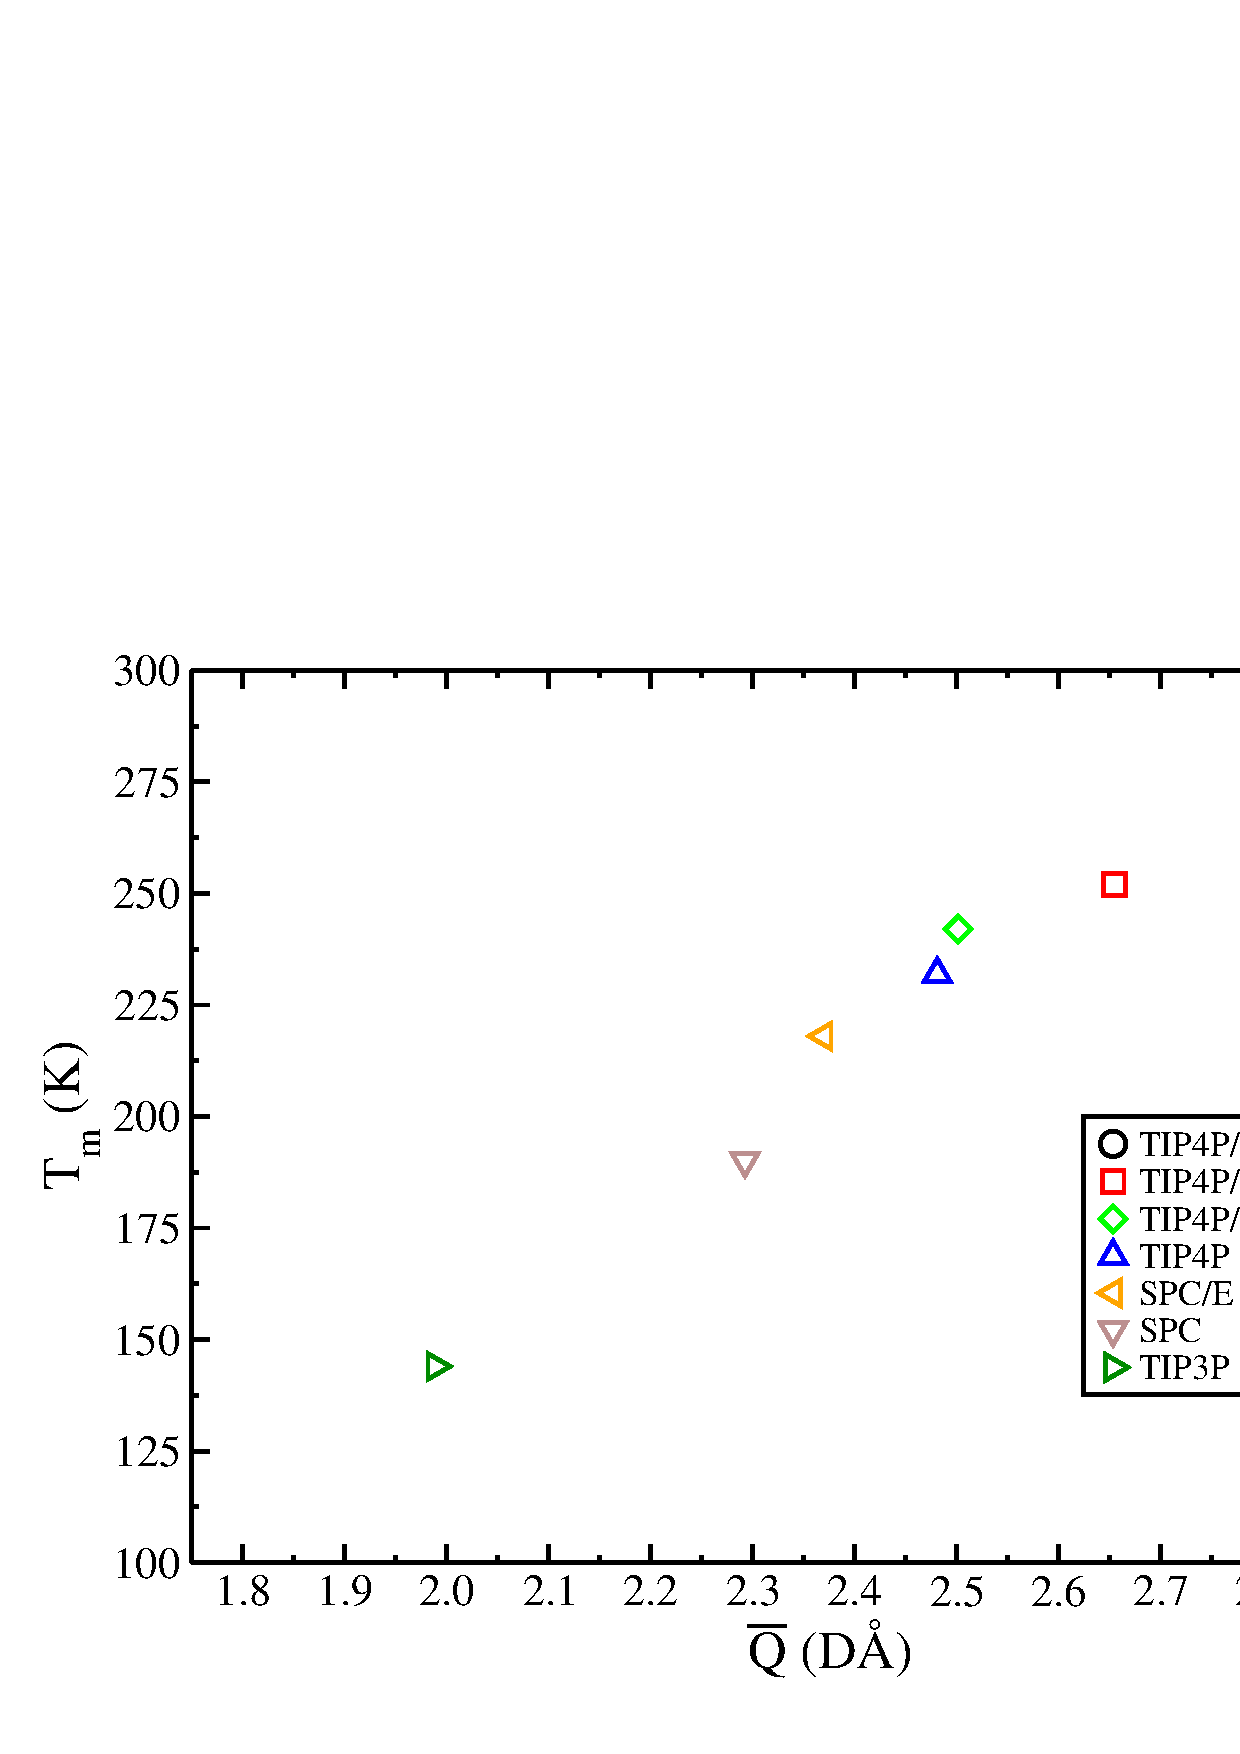
\includegraphics[width=\linewidth]{Figures/Tm_Ih_Qbar_plot.pdf}
\caption{\label{fig:QBar} Melting point for ice I$_h$ of several popular water models as a function of the QBar for the model. We see a strong correlation between a more accurate melting point and a larger value of QBar. We estimate that a QBar of approximately 2.8 D\AA will result in the experimental melting point of 273.15 K. A linear regression of the data resulted in an equation of best fit of $y = 158.89x - 166.83$. From this, we have predicted an optimal QBar to be 2.7690 D\AA~.}
\end{figure}

\begin{figure}[h!]
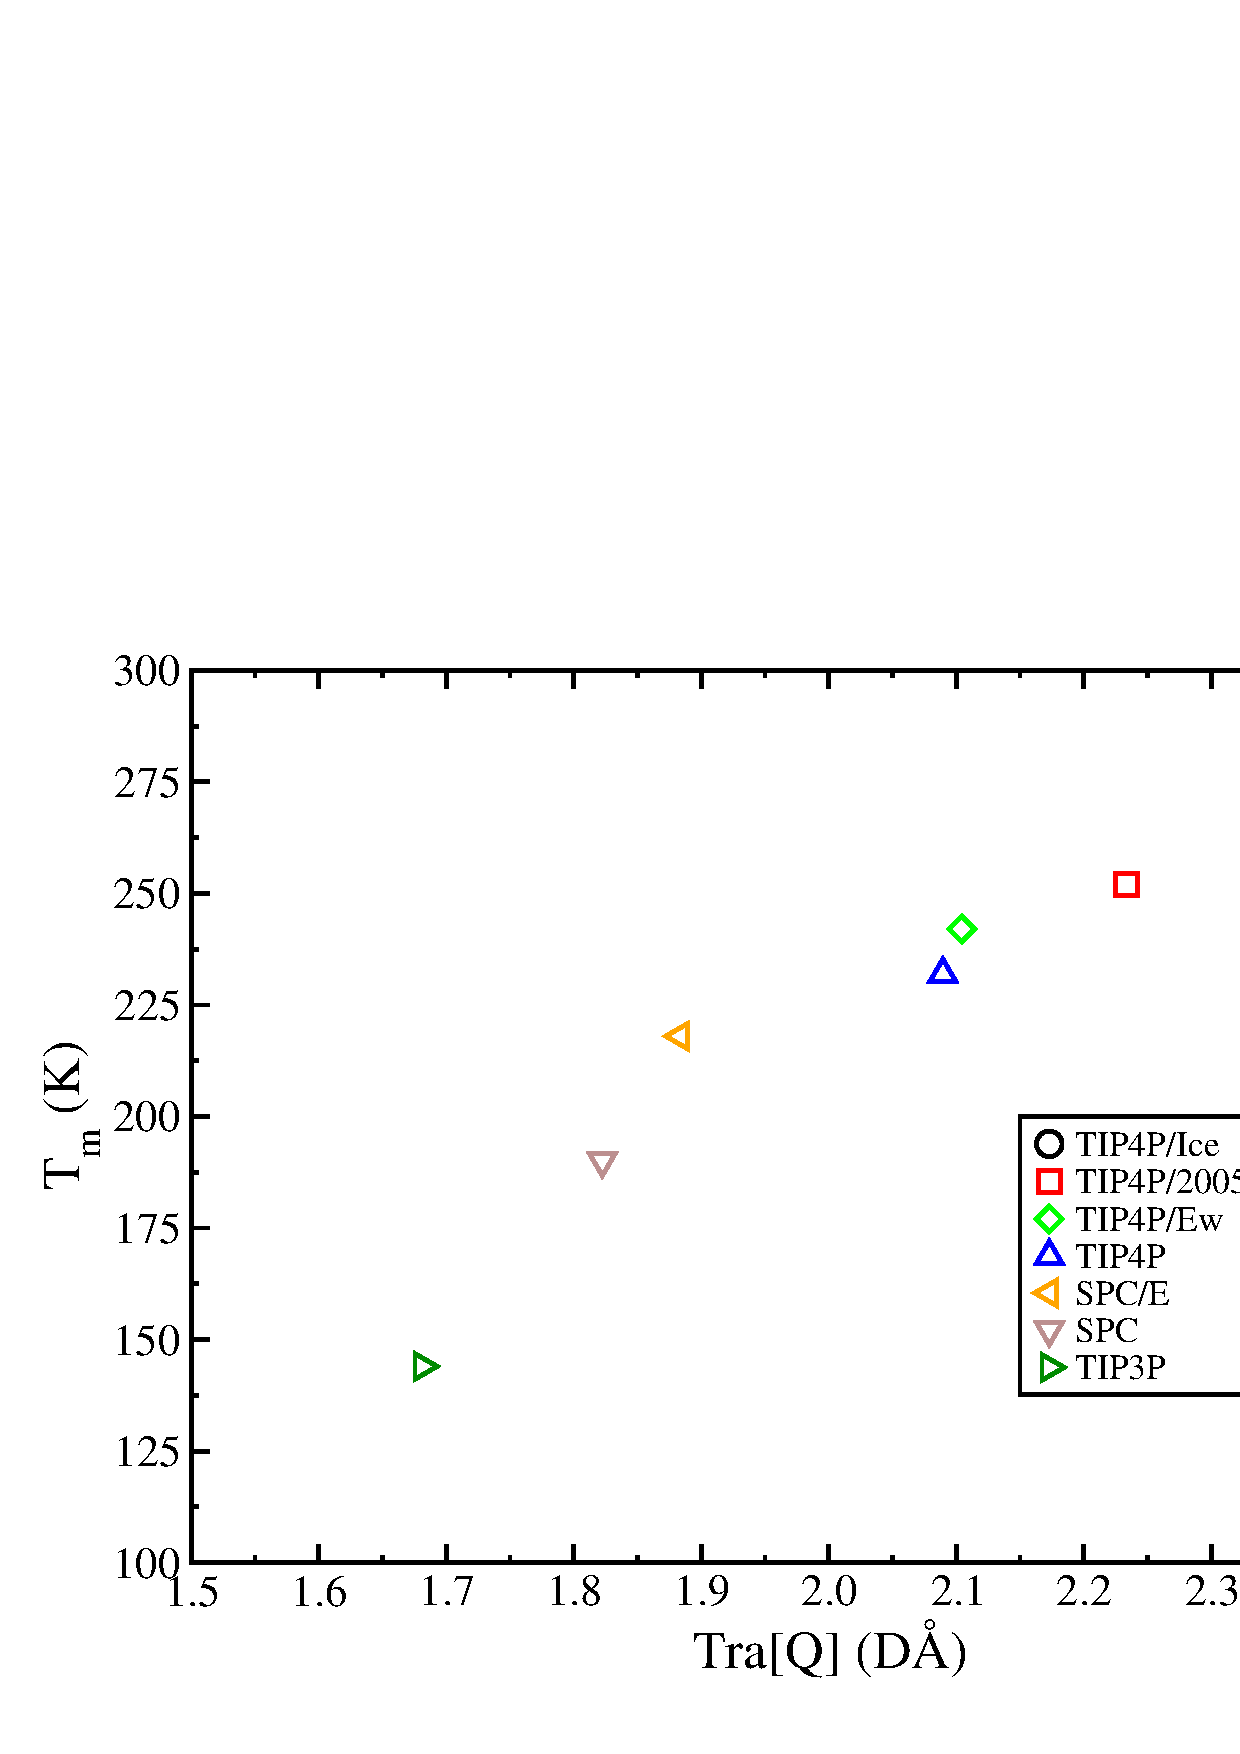
\includegraphics[width = \linewidth]{Figures/Tm_Ih_TraQ_plot.pdf}
\caption{\label{fig:TraQ} Melting point for ice I$_h$ of several popular water models as a function of the trace of the quadrupole tensor for the model. We see a strong correlation between a more accurate melting point and a larger value of the trace. We estimate that a trace of approximately 2.3 D\AA will result in the experimental melting point of 273.15 K.}
\end{figure}



Based on this observation, we have begun work on a 1-site model with intentions
of setting the dipole moment and structuring the quadrupole tensor in such
a way that will give us a ratio of unity. As a starting point, we have 
collapsed the 4-site TIP4P-Ice model\cite{Abascal2005b} onto a 1-site model 
(TIP1P/Ice). The 
geometric parameters, the Lennard-Jones and charges, and the dipole and 
quadrupole elements that have value can be found for both models in 
Table \ref{Geo_Params}, Table \ref{LJq_Params}, and Table \ref{DQ_Params} 
respectively.

\begin{table}[h!]
\begin{tabular}{|c|c|c|c|}
\hline 
& OH bond length \AA & OM bond length \AA & HOH \degree\\
\hline 
TIP4P/Ice & 0.9572 & 0.1577 & 104.52 \\
TIP1P/Ice & - & - & - 			      \\
\hline
\end{tabular}
\caption{Geometric parameters of the TIP4P/Ice and TIP1P/Ice models.}
\label{Geo_Params}
\end{table}

\begin{table}[h!]
\begin{tabular}{|c|c|c|c|c|}
\hline
& $\sigma$ \AA & $\epsilon$ kcal/mol & q$_H$ (e) & q$_M$ (e) \\
\hline 
TIP4P/Ice & 3.1668 & 0.2108509 & 0.5897 & -1.1794 \\
TIP1P/Ice & 3.1668 & 0.2108509 & - & -            \\
\hline
\end{tabular}
\caption{Lennard-Jones and charge parameters of the TIP4P/Ice and TIP1P/Ice models.}
\label{LJq_Params}
\end{table}

\begin{table}[h!]
\begin{tabular} {|c|c|c|c|c|c|}
\hline
& $\mu$ D & Q$_{xx}$ D\AA & Q$_{yy}$ D\AA & Q$_{zz}$ D\AA & Q$_T$ D\AA \\
\hline
TIP4P/Ice & 2.4255966 & 0.0 & 1.62291807 & 0.74278997 & 2.434 \\
TIP1P/Ice & 2.4255966 &0.0 & 1.62291807 & 0.74278997 &2.434 \\
\hline
\end{tabular}
\caption{Dipole and quadrupole parameters for the TIP4P/Ice and TIP1P/Ice models.}
\label{DQ_Params}
\end{table}


\section{TIP1P/Ice}
\subsection{Gas Phase Dimer}
This section contains details and graphs of the attempts to tune the TIP1P/Ice
model to the experimental and ab initio predicted results for the gas phase
water dimer. In order to tune the TIP1P/Ice model, we are going to calculate 
the geometry of the gas phase water dimer as shown in Figure 
\ref{fig:dimer}\cite{Yu2004}.

\begin{figure}[h!]
\includegraphics[width = \linewidth]{Figures/dimer.pdf}
\caption{\label{fig:dimer} The gas phase water dimer geometry.}
\end{figure}

There are three values of interest for our characterization of the water dimer.
The first is the oxygen-oxygen separation distance, R$_{OO}$. The other two
parameters of the dimer are the two angles, $\theta$ and $\phi$. These angles
are taken from the HOH bisector to the R$_{OO}$ vector. While the length
of the R$_{OO}$ vector will be dependent on the magnitude of the dipole and 
quadrupole moments, the relative contributions of Q$_{xx}$, Q$_{yy}$, and
Q$_{zz}$ will strongly influence the angles. We also expect that the 
Lennard-Jones parameter $\sigma$ will strongly influence the magnitude of
the R$_{OO}$ vector.
The experimentally measured and computationally predicted values for the 
geometry of the water
dimer can be found in Table \ref{dimer_geo}. Also in Table \ref{dimer_geo}, we
see the geometry parameters computed at 0.1 K for the TIP4P/Ice and TIP1P/Ice
models.

\begin{table}[h!]
\begin{tabular}{|c|c|c|c|}
\hline
& R$_{OO}$ (\AA) & $\theta$ (\degree)& $\phi$ (\degree) \\
\hline
Expt.     & 2.95 & 51 $\pm$ 10 & 57 $\pm$ 10 \\ 
Ab initio & 2.91 & 56    & 58    \\
TIP4P/Ice & 2.79 & 52.52 & 43.17 \\
TIP1P/Ice & 2.83 & 40.56 & 36.59 \\
\hline
\end{tabular}
\caption{Geometric parameters of the TIP4P/Ice and TIP1P/Ice gas phase water dimer. Ab initio and Expt. values were taken from another source\cite{Yu2004}.}
\label{dimer_geo}
\end{table}

\subsubsection{Testing Electrostatic Cutoff}
First we will see if we can recover the TIP4P/Ice dimer geometry by decreasing
damping $\alpha$ to 0.05 \AA$^{-1}$ and vary the cutoff radius for the
electrostatics. In Figure \ref{fig:rcut}, we see that with very small damping 
$\alpha$, increasing the cutoff radius of the potential
does not recover the TIP4P/Ice calculated geometry.

\begin{figure}[h!]
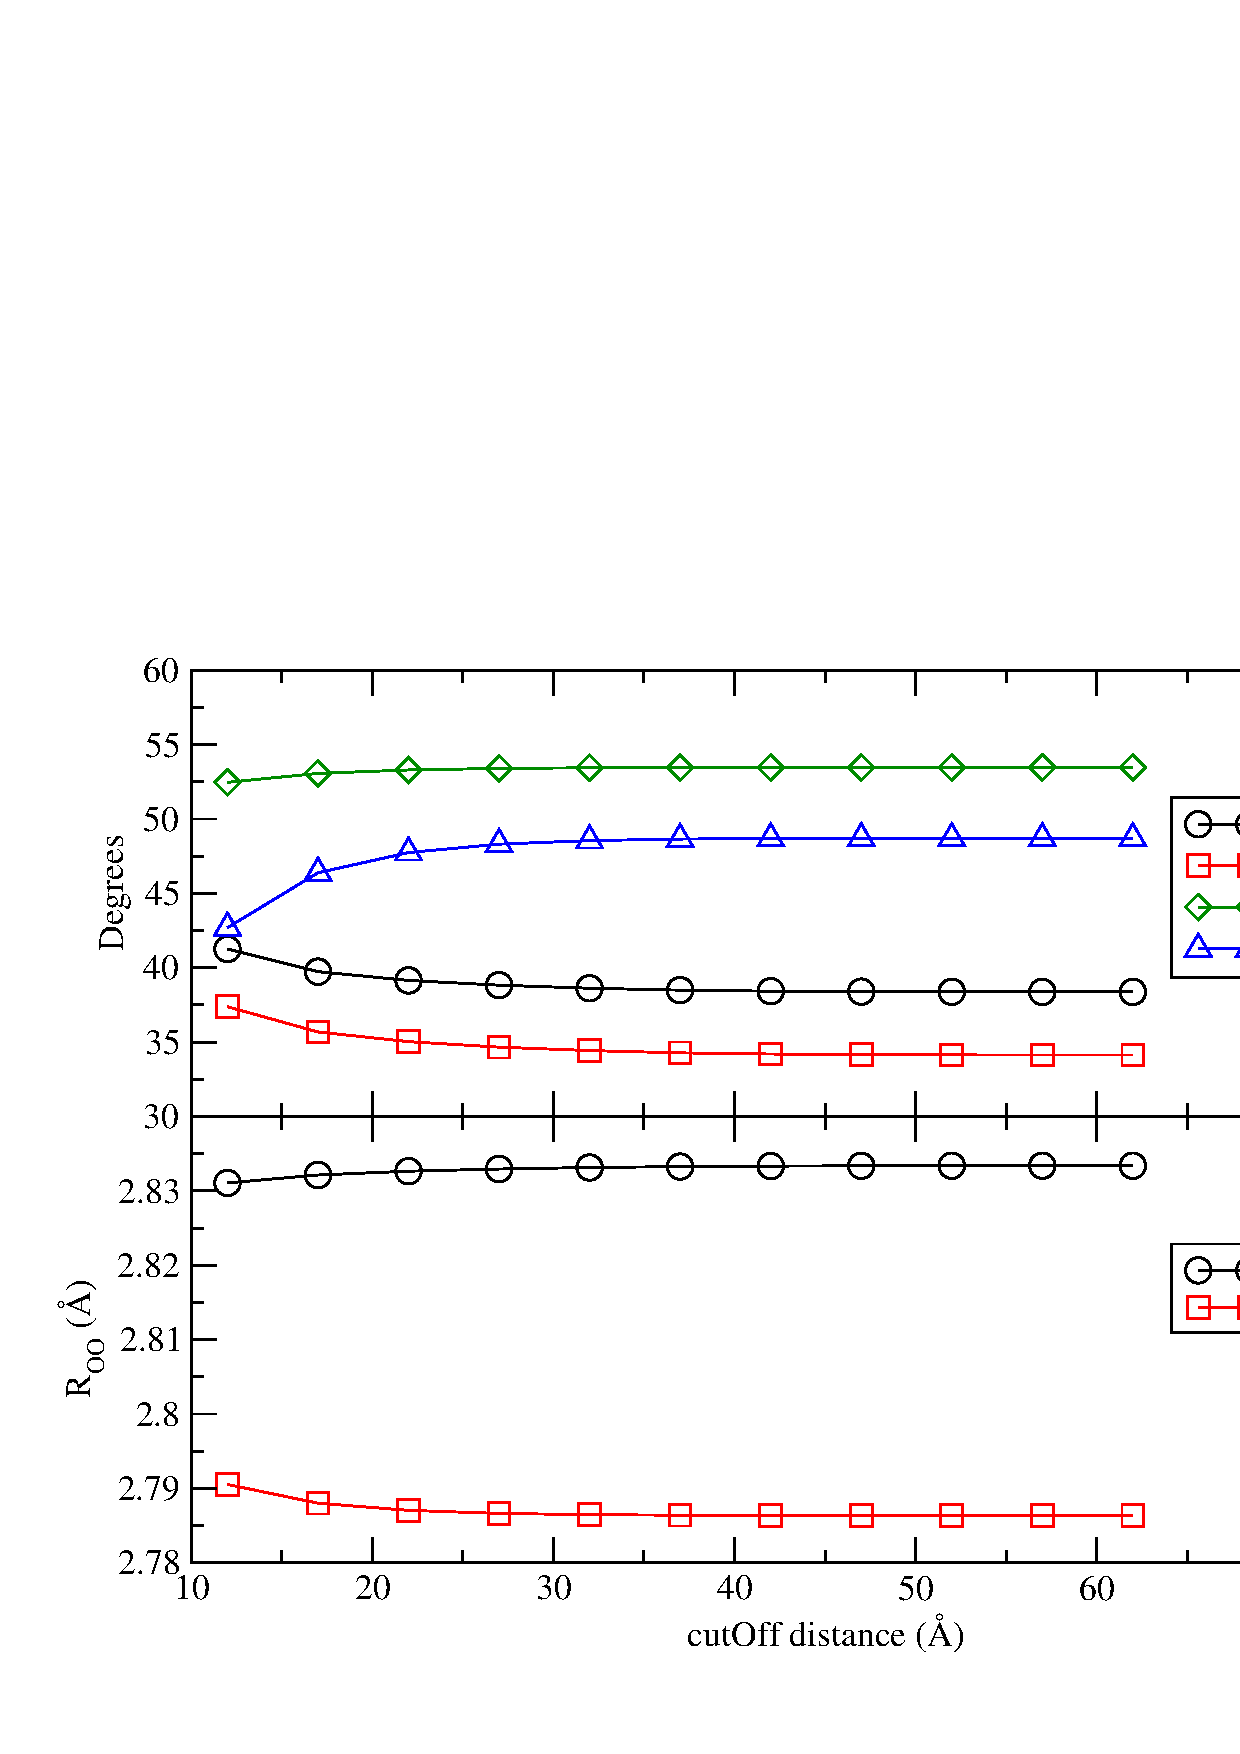
\includegraphics[width = \linewidth]{Figures/Test17_plot.pdf}
\caption{\label{fig:rcut} Damping $\alpha$ set to 0.05 \AA$^{-1}$ and the simulation box was $300\times300\times300$ \AA~.}
\end{figure}

\subsubsection{Varying Lennard-Jones Parameters}
In our initial test, as seen in Figure \ref{fig:Sigma}, the Lennard-Jones 
parameter $\sigma$ was varied 
while holding the other parameters of the TIP1P/Ice model constant. We see that
the ab. initio predicted R$_{OO}$ separation distance of 2.91 \AA is obtained
when $\sigma$ is set to approximately 3.25 \AA . However, the two angles 
$\theta$ and $\phi$ tend to decrease with increasing values of $\sigma$, 
and result in values of about 36\degree and 31\degree, which is in poor 
agreement with the ab. initio calculations. Also, changing the Lennard-Jones
parameter $\sigma$ will drastically alter the condensed phase properties
of the model. Namely, the radial distribution function is very sensative to
$\sigma$. The location of the first solvation shell can be tuned by $\sigma$,
so we will initially retain the TIP4P/Ice model's value of 3.1668 \AA~ and vary
it later if the radial distribution function is off.


\begin{figure}[h!]
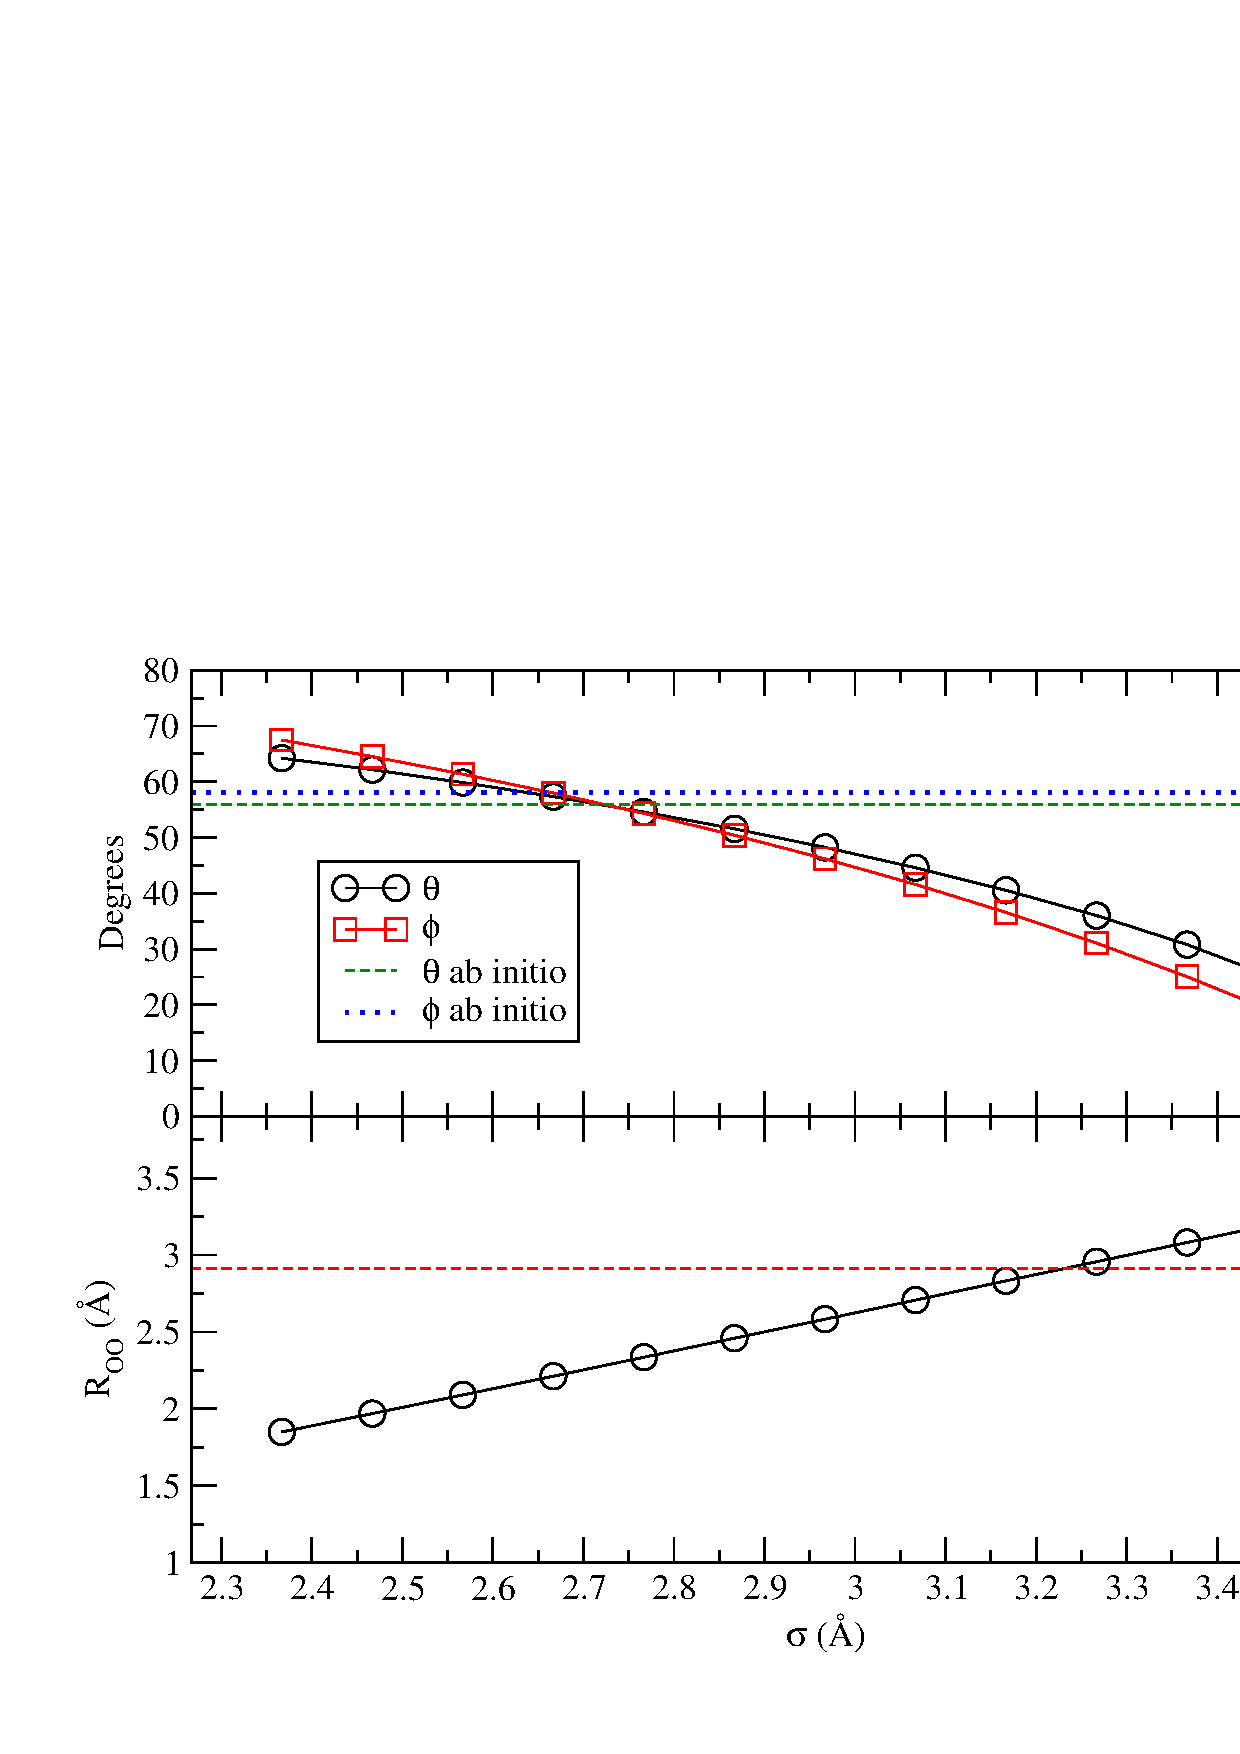
\includegraphics[width = \linewidth]{Figures/Test1_plot.pdf}
\caption{\label{fig:Sigma} The Lennard-Jones parameter $\sigma$ was varied while holding the other parameters of the TIP1P/Ice model constant.}
\end{figure}


Next, we will vary the Lennard-Jones parameter $\epsilon$, as seen in 
Figure \ref{fig:Epsilon}. We see that the ab. initio calculated value 
of R$_{OO}$ 
distance of about 2.91 \AA is achieved when $\epsilon$ is set to 
approximately 0.275 kcal/mol. However, both $\theta$ and $\phi$ tend to 
decrease with increasing $\epsilon$, and the resulting values for the two 
angles at this value of $\epsilon$ are approximately 38\degree and 33\degree,
which are again far from the predicted values. Changing $\epsilon$ is not a
great way to parameterize the model though, and we will avoid doing so as much
as possible.

\begin{figure}[h!]
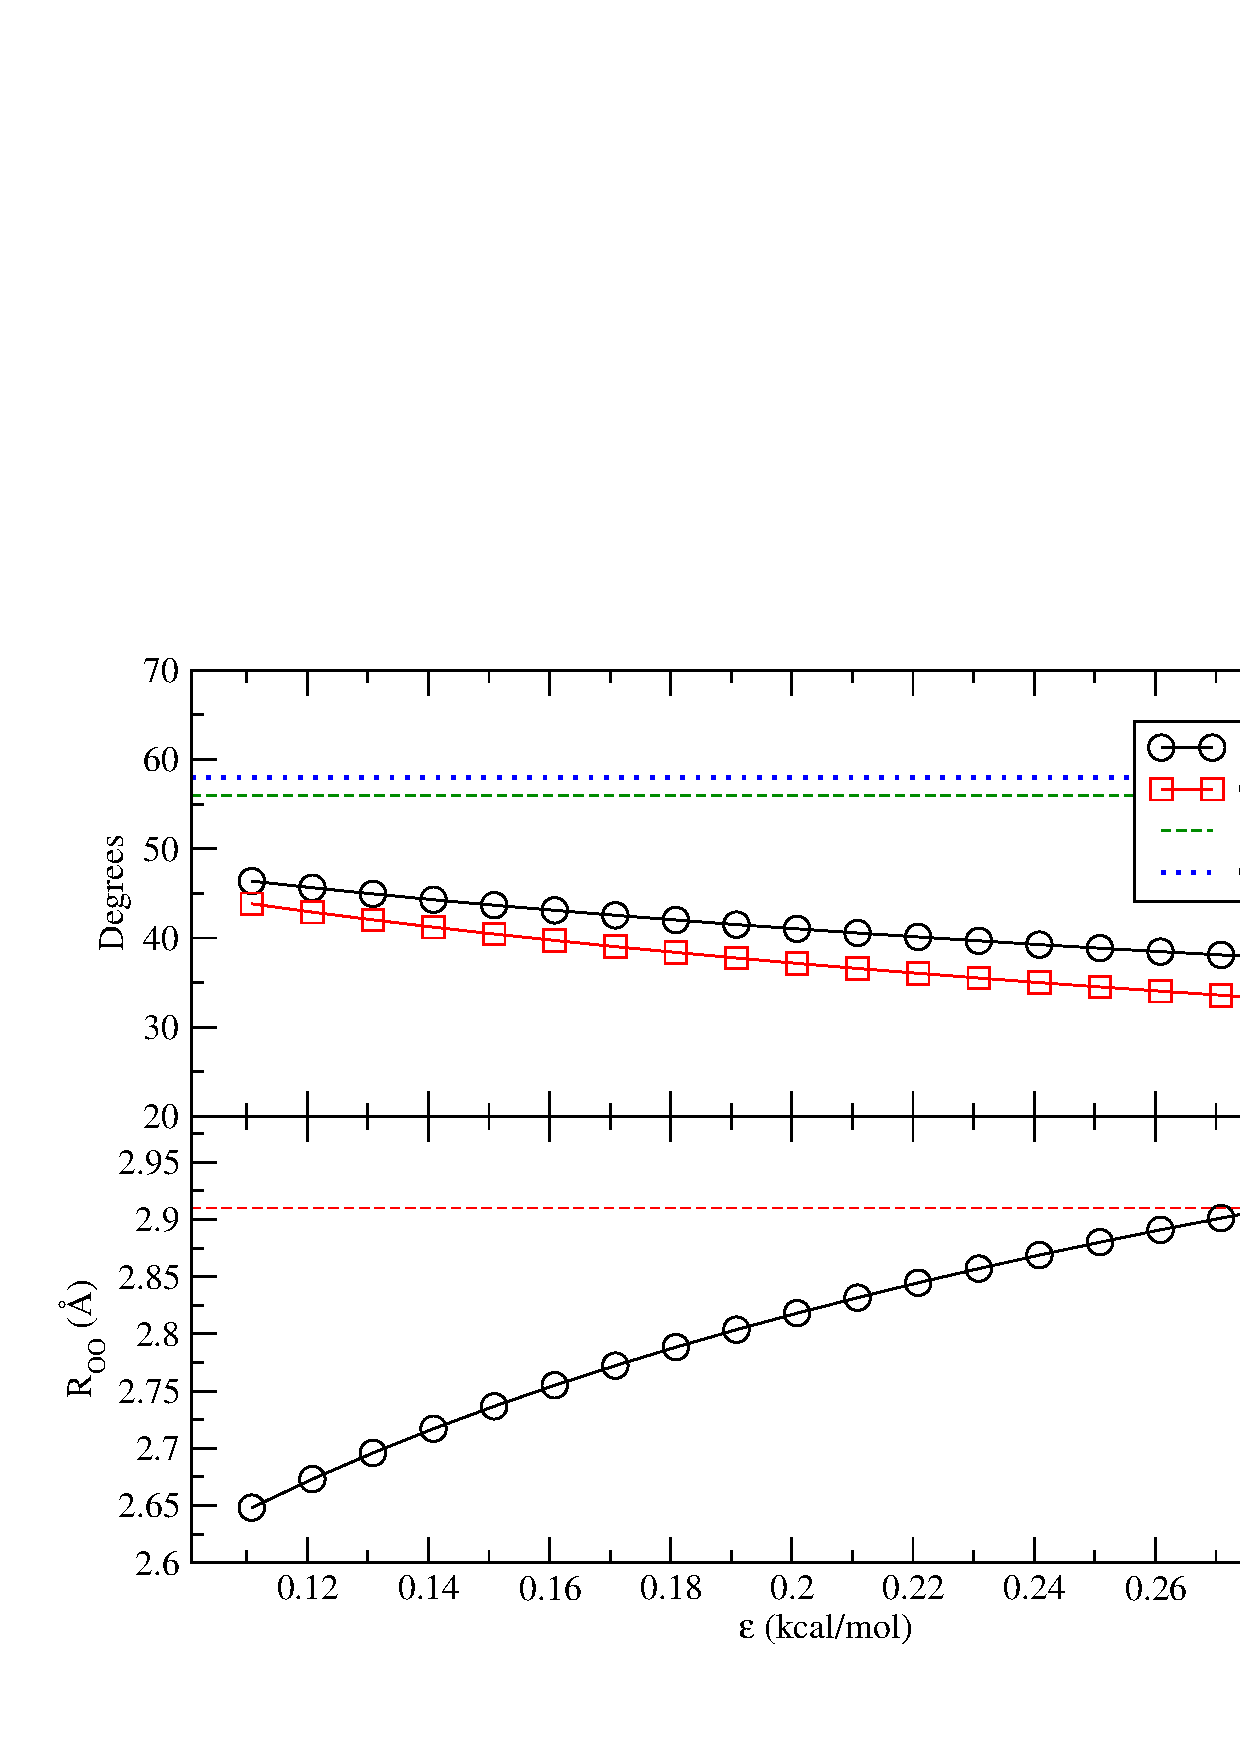
\includegraphics[width = \linewidth]{Figures/Test2_plot.pdf}
\caption{\label{fig:Epsilon} The Lennard-Jones parameter $\epsilon$ was varied while holding the other parameters of the TIP1P/Ice model constant.}
\end{figure}

\subsubsection{Varying Damping $\alpha$}
Having changed both the Lennard-Jones parameters independently and not 
achieving the desired values for the separation distance or angles of the
gas phase water dimer, the next natural parameter of the TIP1P/Ice model to 
vary would be the dipole or quadrupole moment. Before doing so, however, 
we will vary the damping $\alpha$ value which effects how the electrostatics
are calculated in OpenMD\cite{openmd}. In Figure \ref{fig:Dalpha}, we see that
R$_{OO}$ is minimally effected by varying damping $\alpha$ for small values of
$\alpha$. For values larger than about 0.25 \AA$^{-1}$, the dimer separation
distance decreases slighty. However, the ab. initio calculated distance
is not recovered by varying damping $\alpha$ alone. The angles $\theta$ and
$\phi$ also do not converge on the ab. initio predicted values over the range
of damping $\alpha$ investigated here. After talking with Madan, damping
$\alpha$ values of about 0.1 \AA$^{-1}$ are suitable for handling the 
calculation of dipoles and quadrupoles, which is the value that has been used
in all other Tests shown here.

\begin{figure}[h!]
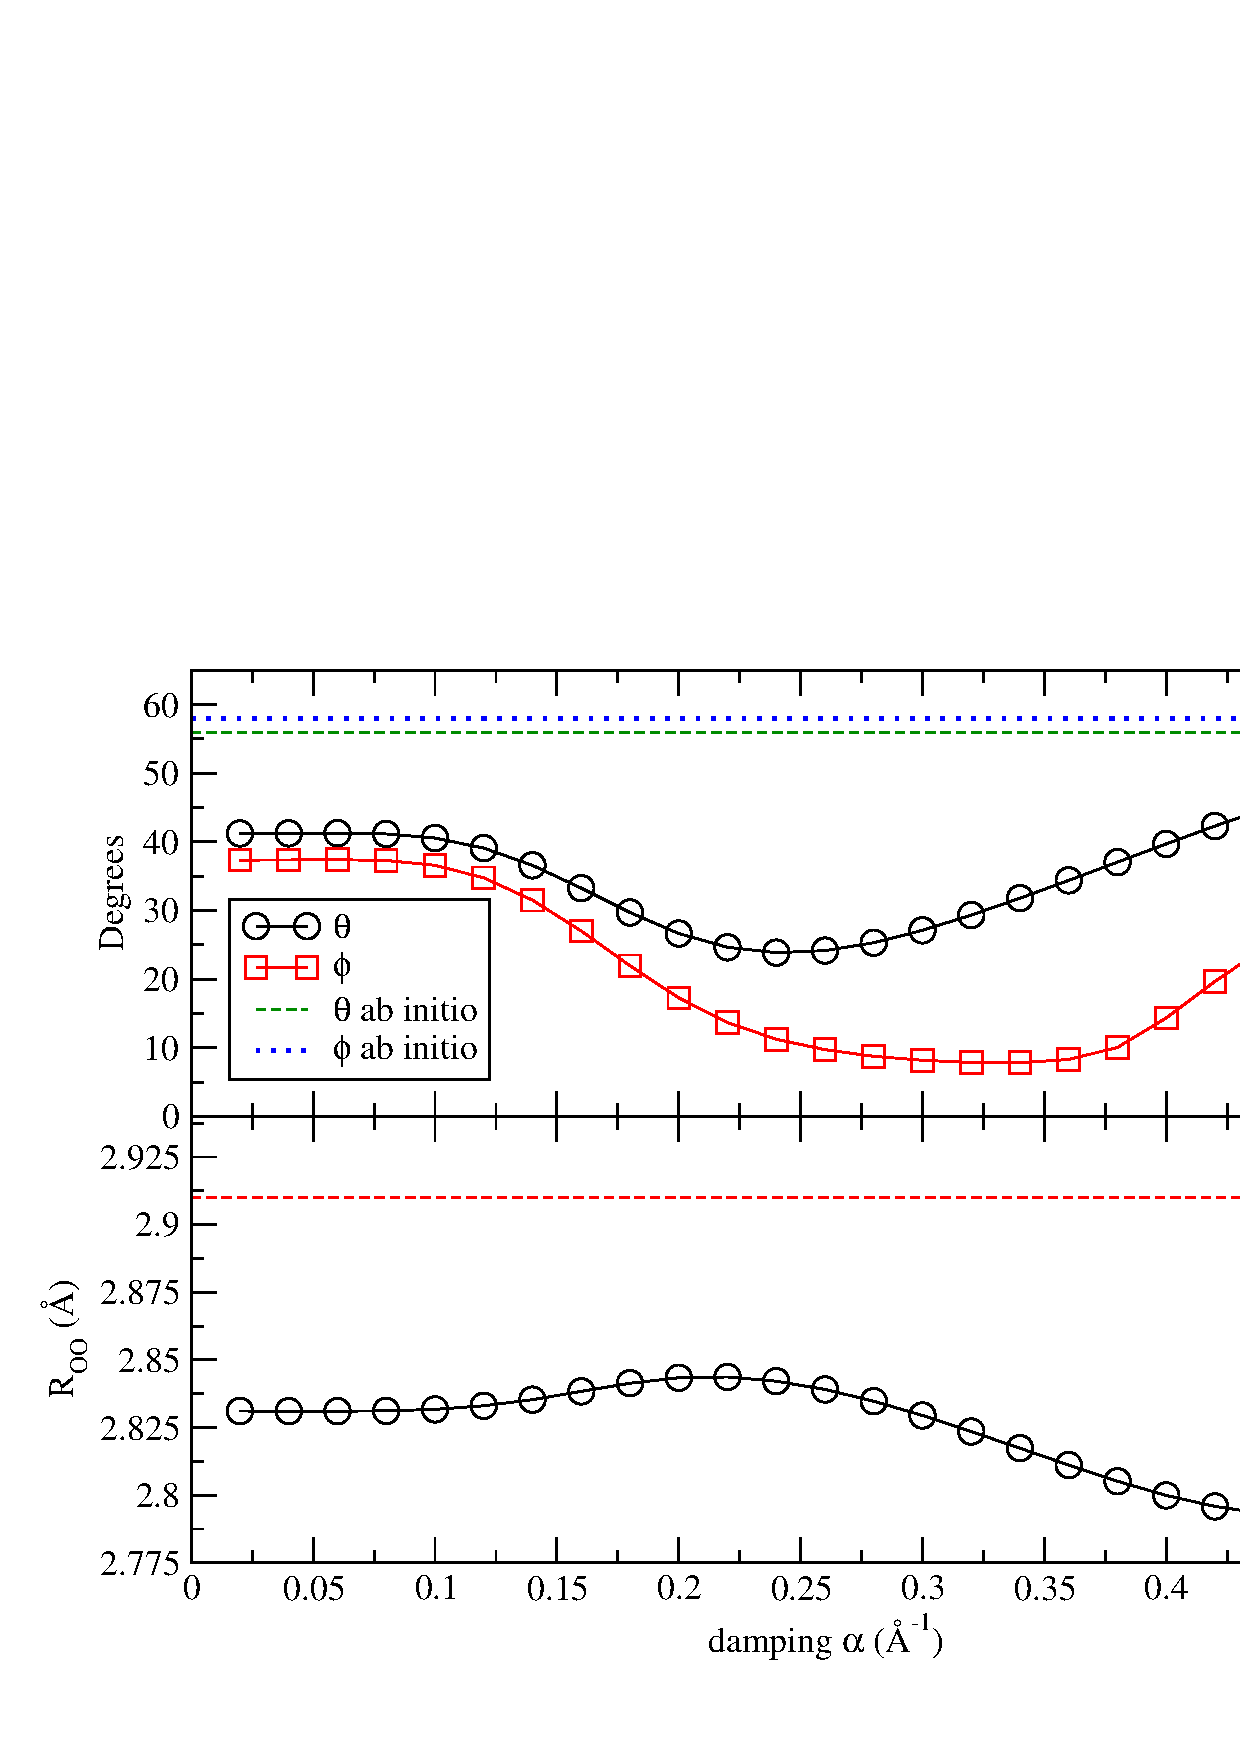
\includegraphics[width = \linewidth]{Figures/Test3_plot.pdf}
\caption{\label{fig:Dalpha} Damping $\alpha$ was varied while holding the otherparameters of the TIP1P/Ice model constant.}
\end{figure}


\subsubsection{Varing the Quadrupole: Introduction of Q$_{xx}$}
A possible reason we have not been able to capture the correct gas phase water
dimer geometry by modifying the Lennard-Jones parameters, may be due to the
initial construction of the quadrupole tensor for the TIP1P/Ice model. In this
model,
as with all planar water models, one of the quadrupole tensor's main diagonal
elements will be zero, given intelligent choice of origin for the coordinate
system. In our construction, this is the Q$_{xx}$ term, as seen in Table
\ref{DQ_Params}. In the following Tests, we will try to incorporate 
the quadrupole moment of the $x$-dimension into our model.

We will consider varying the quadrupole tensor elements of the TIP1P/Ice
model while holding all other parameters constant. This requires special 
consideration though, as we may not want to deviate from TIP1P/Ice's Q$_T$
or $TrQ$ initial values. We initially will consider a Test in which Q$_T$ is 
conserved while varying Q$_{xx}$ by the following constraints. 

\begin{equation}
Q_{yy}^{'} = Q_{yy} + \lambda
\end{equation} 
\begin{equation}
Q_{xx}^{'} = Q_{xx} - \lambda
\end{equation}

While Q$_T$ is conserved in this Test, $TrQ$ is not. In Test 4, seen in Figure
\ref{fig:Qxx}, a similar behavior is apparent as we vary the value of Q$_{xx}$.
Here the $TrQ$ is not conserved, and we have plotted the same data from 
Figure \ref{fig:Qxx} by the $TrQ$ in Figure \ref{fig:Qxx2}. In both graphs,
However, the angle $\phi$ is larger
than $\theta$ at negative values of Q$_{xx}$ here while $\theta$ was larger 
than $\phi$ when we varied Q$_{zz}$. Again no value of Q$_{xx}$ results in the
R$_{OO}$ separation predicted by the ab initio calculations. The angles
also cross over one another as seen previously.  

\begin{figure}[h!]
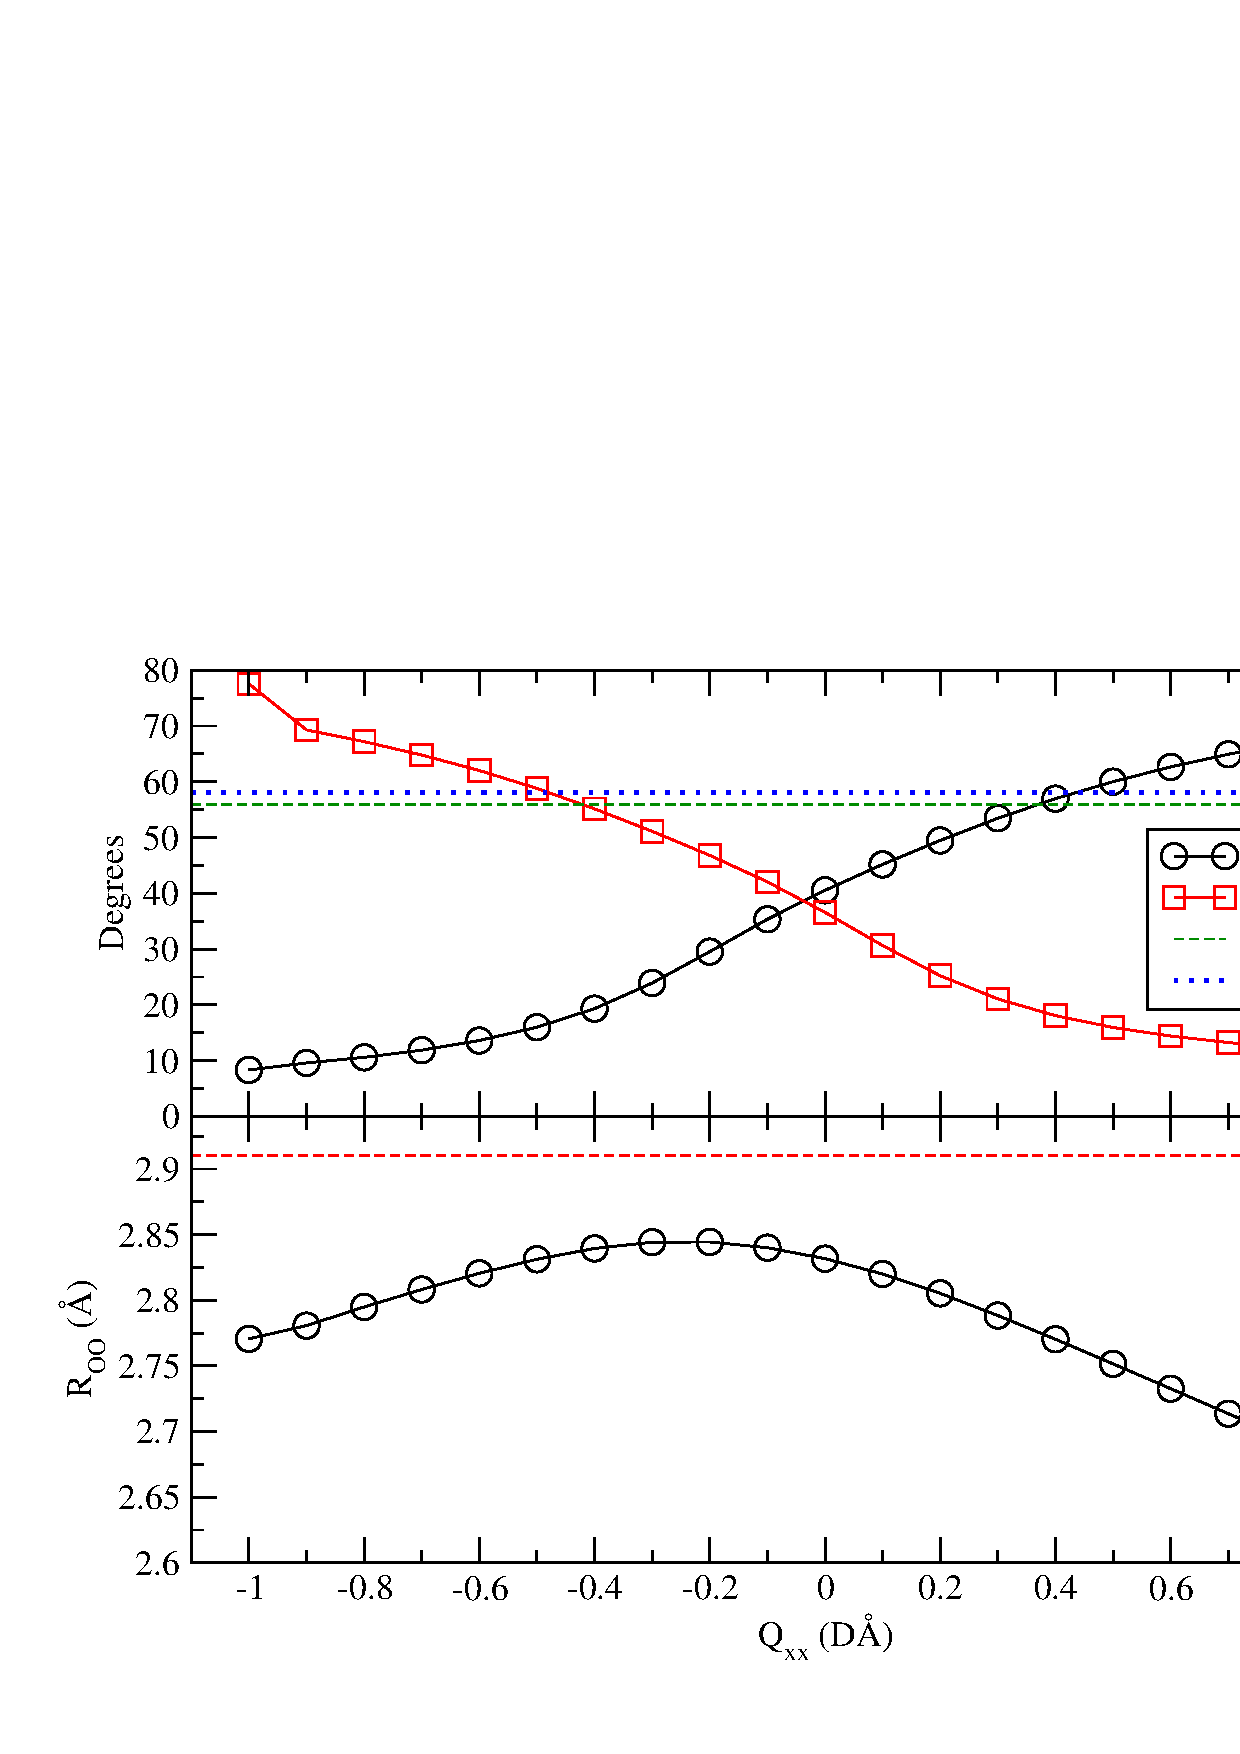
\includegraphics[width = \linewidth]{Figures/Test4_plot.pdf}
\caption{\label{fig:Qxx} The Q$_{xx}$ components of the traced quadrupole tensor were varied while simultaneously adjusting the Q$_{yy}$ component such that the Q$_T$ value for the TIP1P/Ice model was held constant. All other parameters were also held constant and equal to the TIP1P/Ice parameters during this test.This means that $Tr(Q)$ varied since the $Q_{zz}$ component was not adjusted as$Q_{xx}$ was varied.}
\end{figure}


\begin{figure}[h!]
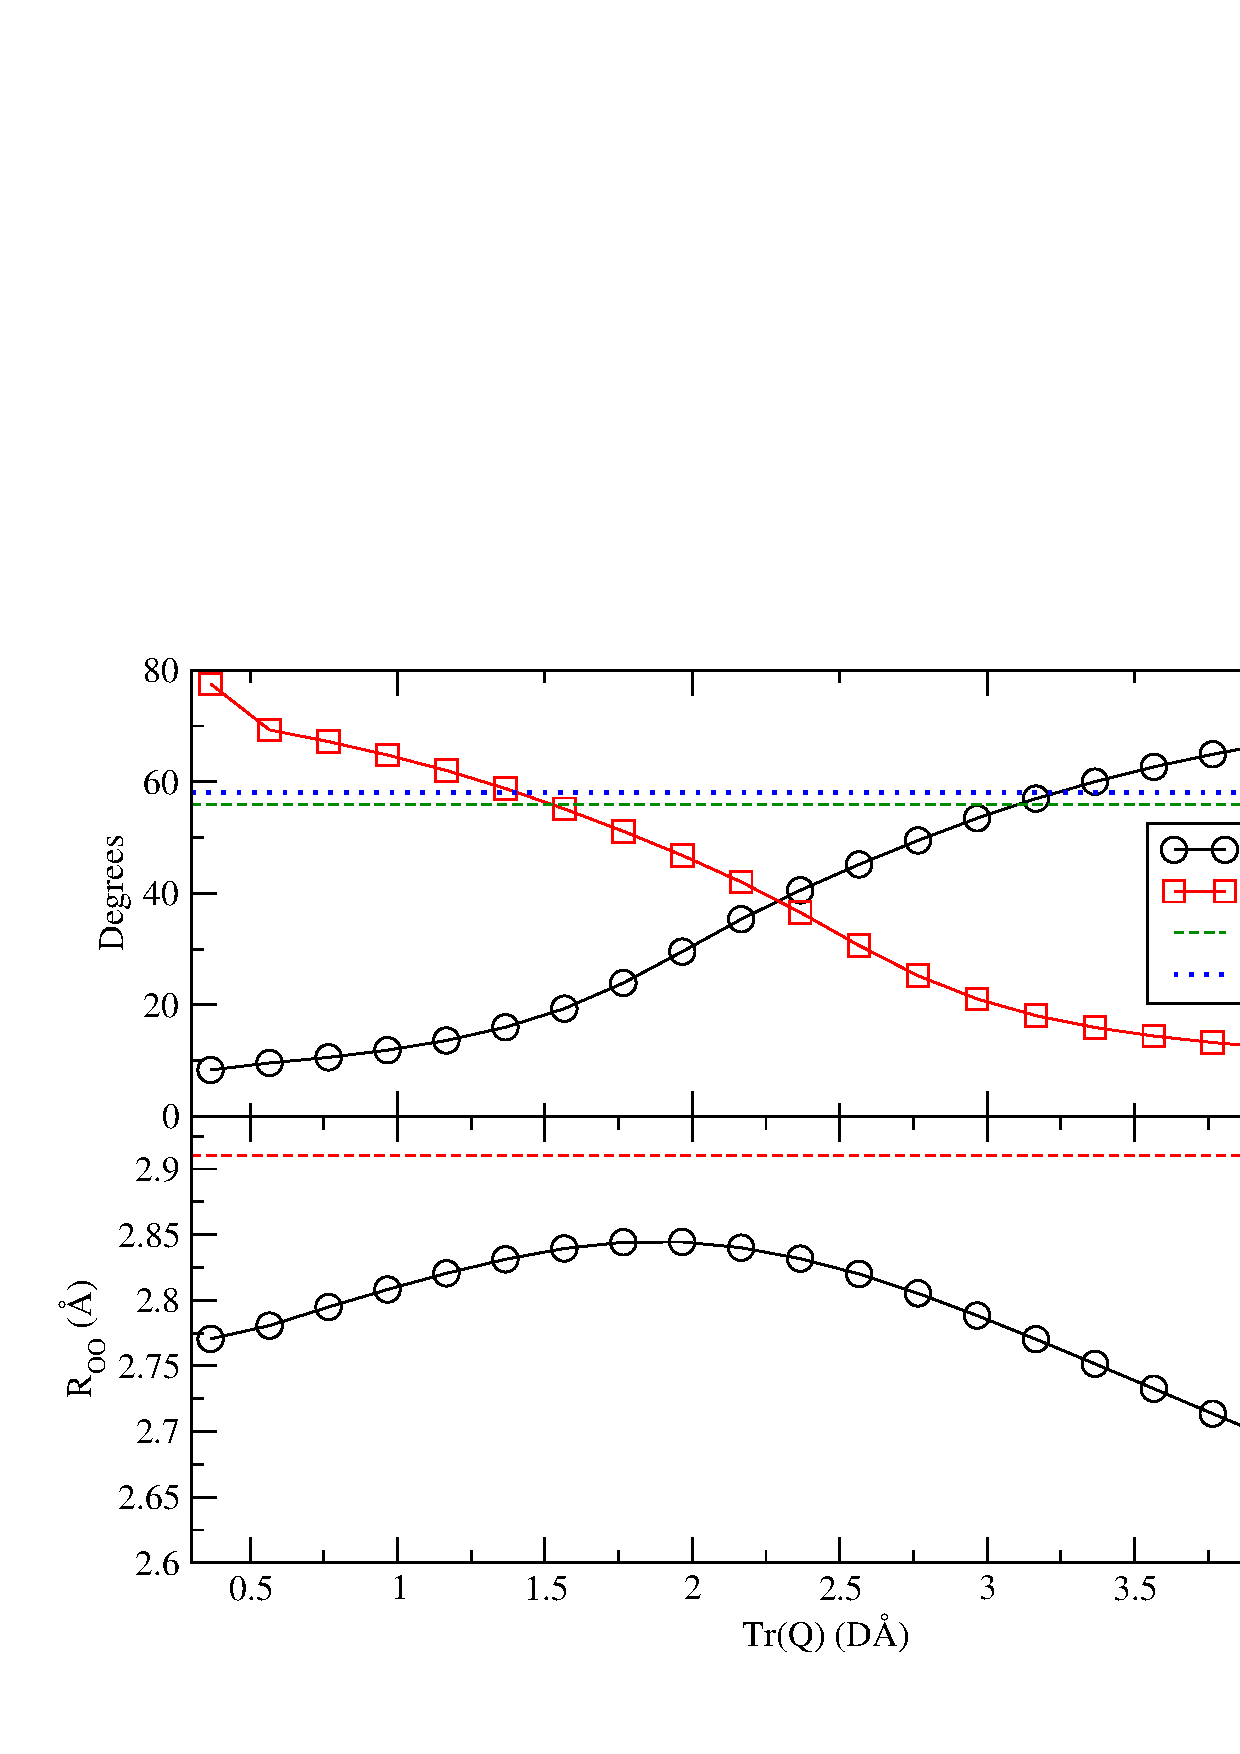
\includegraphics[width = \linewidth]{Figures/Test4_plot2.pdf}
\caption{\label{fig:Qxx2} The same data as plotted in Figure \ref{fig:Qxx}, nowplotted as a function of the $TrQ$.}
\end{figure}

In the next Test, we allow Q$_{xx}$ to vary as in the previous Test, however
we now change Q$_{zz}$ in such a way to keep the $TrQ$ constant to it's 
initial value, as well as varying Q$_{yy}$ in order to conserve Q$_T$. 
In Figure \ref{fig:Qxx3}, we see that the dimer separation 
distance R$_{OO}$ peaks at a Q$_{xx}$ value of about -0.1 D\AA~, and the angles
have the right ordering for which is larger at this value. However, neither 
the R$_{OO}$ or the angles are the correct numerical values as predicted by
the ab initio calculations. Therefore, we will increase the value of 
$\sigma$ to 3.2668 \AA~, determined by the R$_{OO}$ distance in Figure 
\ref{fig:Sigma}. The results of doing so are shown in Figure \ref{fig:Qxx4}. 
Here we see that we have overshot the value of R$_{OO}$, and that our range of
values of Q$_{xx}$ is still quite large. Thus in the next Test, shown in
Figure \ref{fig:Qxx5}, we have adapted a $\sigma$ value of 3.2268 \AA~. Here we
see that we can accurately achieve the correct ordering of the angles, and
approximately 
the correct value for R$_{OO}$ at Q$_{xx}$ values of about -0.02 D\AA~. 

\begin{figure}[h!]
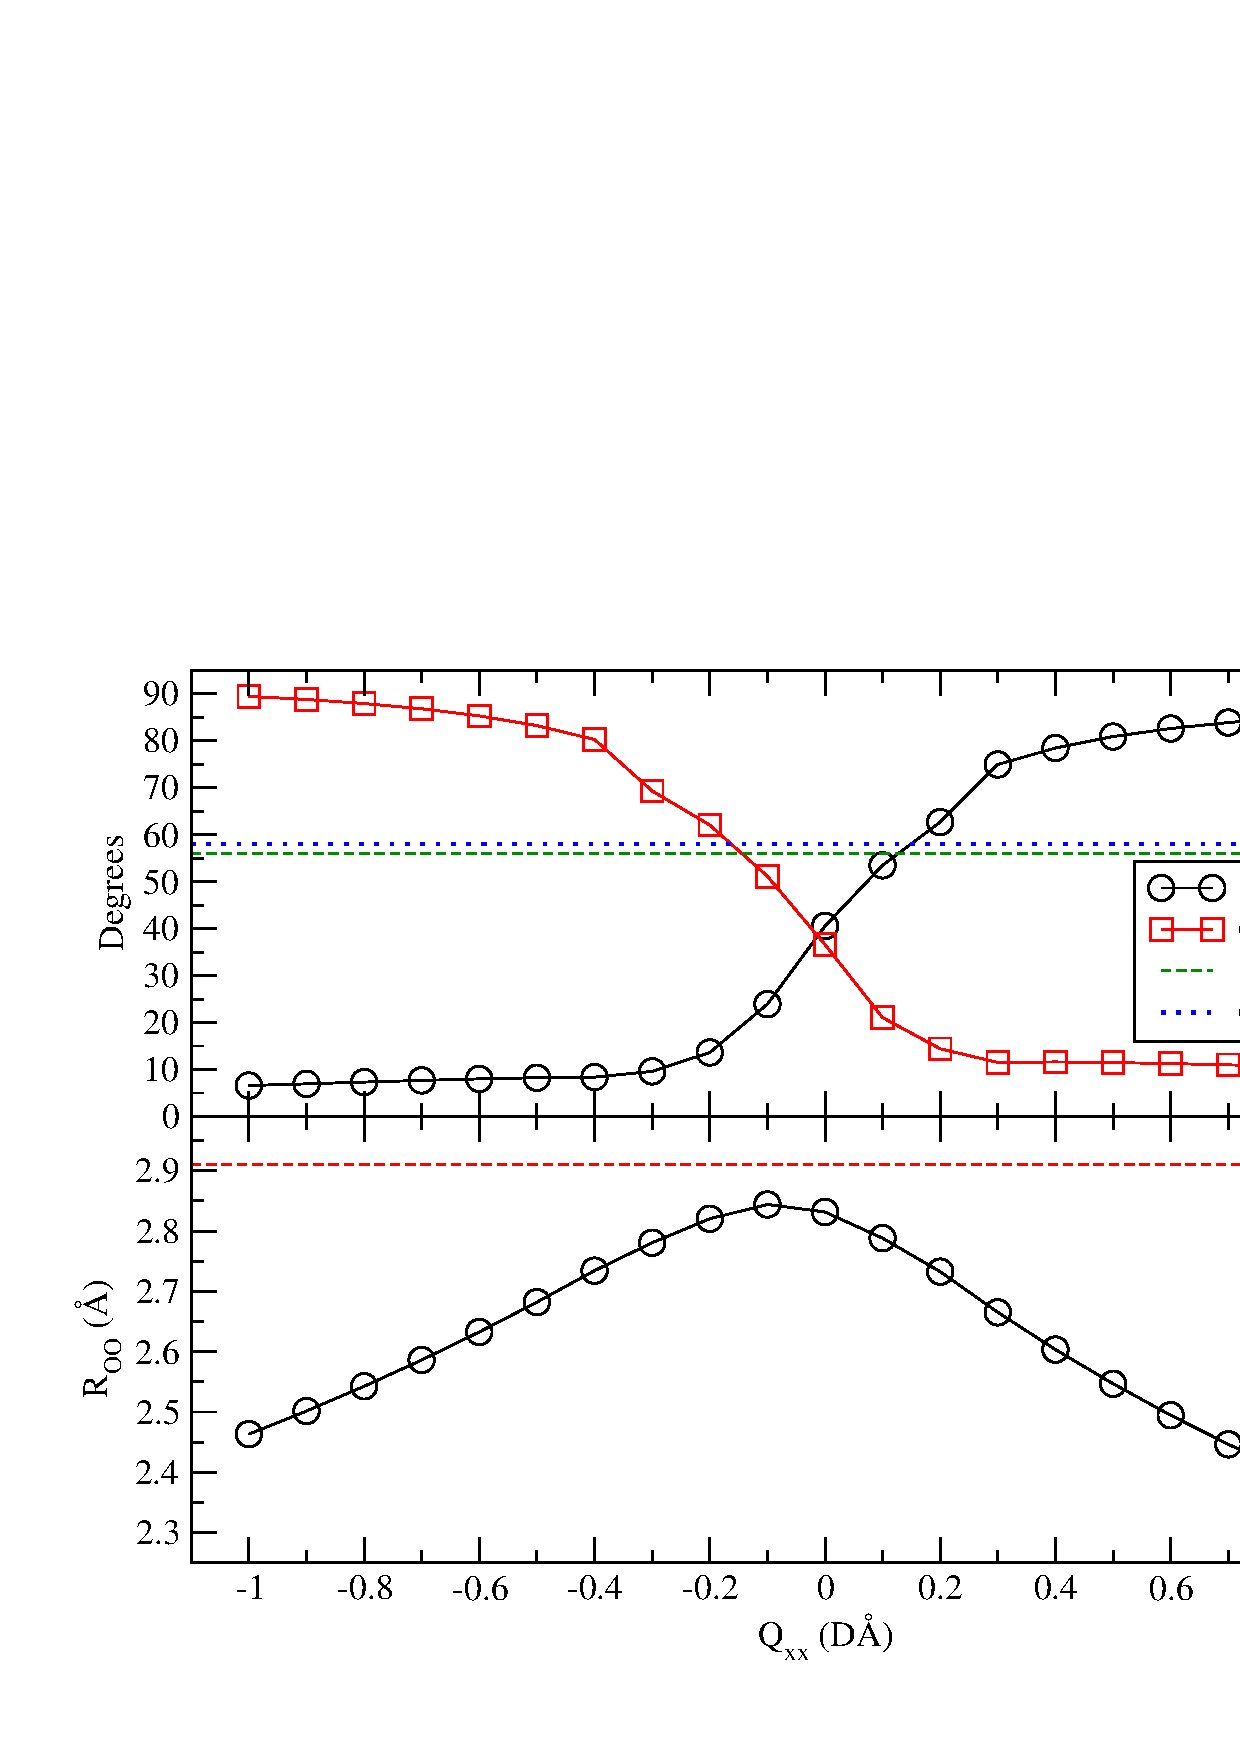
\includegraphics[width = \linewidth]{Figures/Test5_plot.pdf}
\caption{\label{fig:Qxx3} The Q$_{xx}$ components of the traced quadrupole tensor were varied while simultaneously adjusting the Q$_{yy}$ component such that the  Q$_T$ value for the TIP1P/Ice model was held constant. The Q$_{zz}$ component of the quadrupole tensor was also varied in such a way as to keep the $Tr(Q)$ held constant to the TIP1P/Ice value. We see here that the angles cross overone another as in Figure \ref{fig:Qxx}.}
\end{figure}

\begin{figure}[h!]
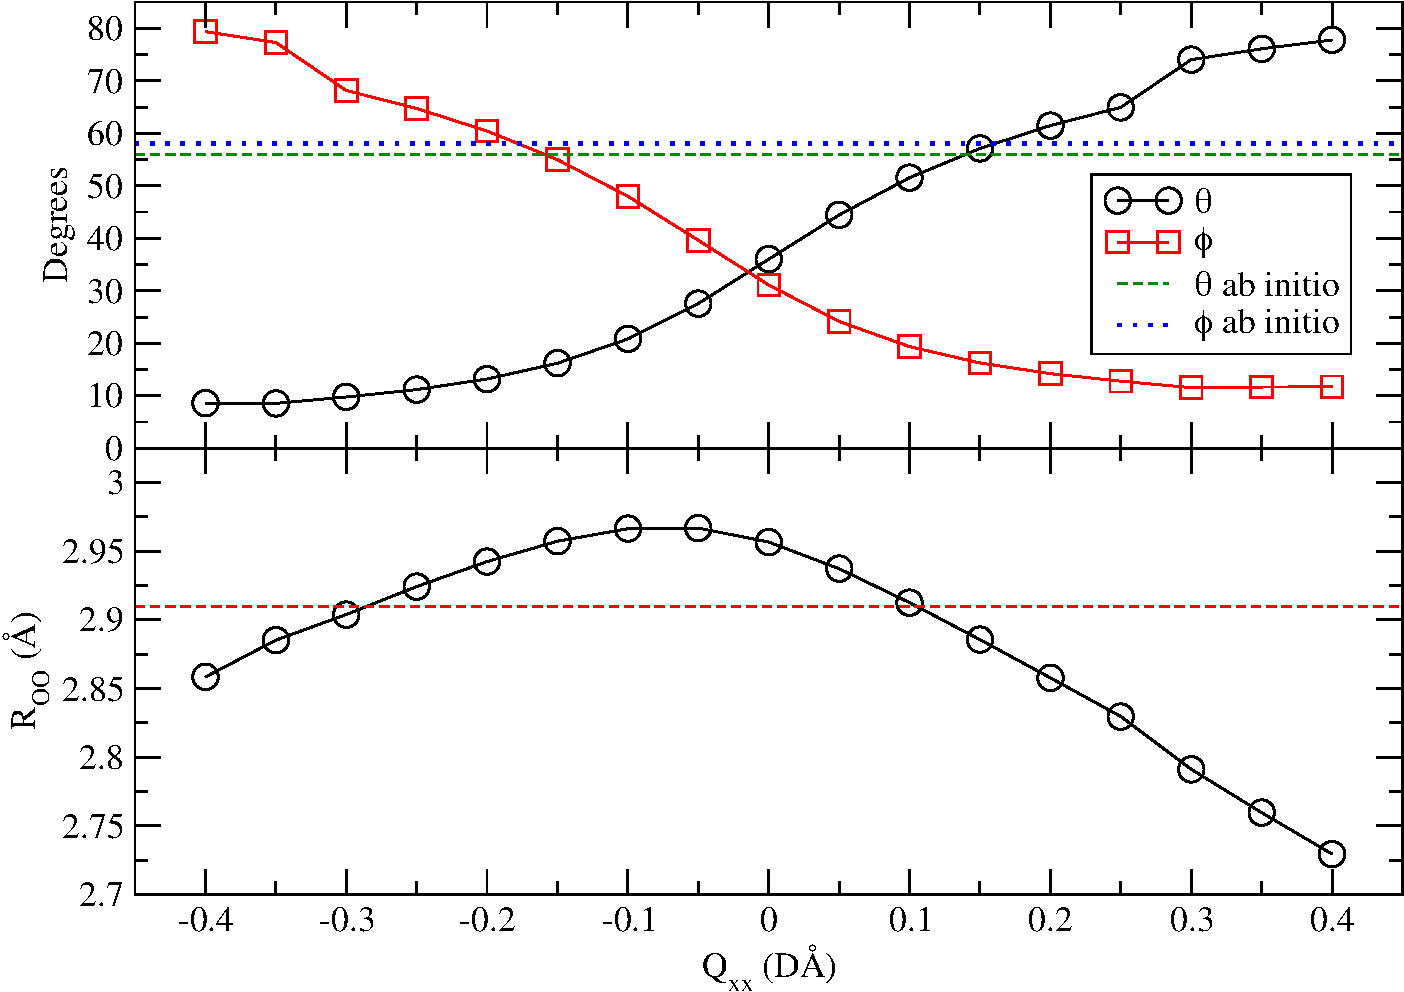
\includegraphics[width = \linewidth]{Figures/Test6_plot.pdf}
\caption{\label{fig:Qxx4} Setting $\sigma$ to 3.2668 \AA~, vary Q$_{xx}$ while simultanesouly adjusting Q$_{yy}$ and Q$_{zz}$ to conserve Q$_T$ and $TrQ$.}
\end{figure}

\begin{figure}[h!]
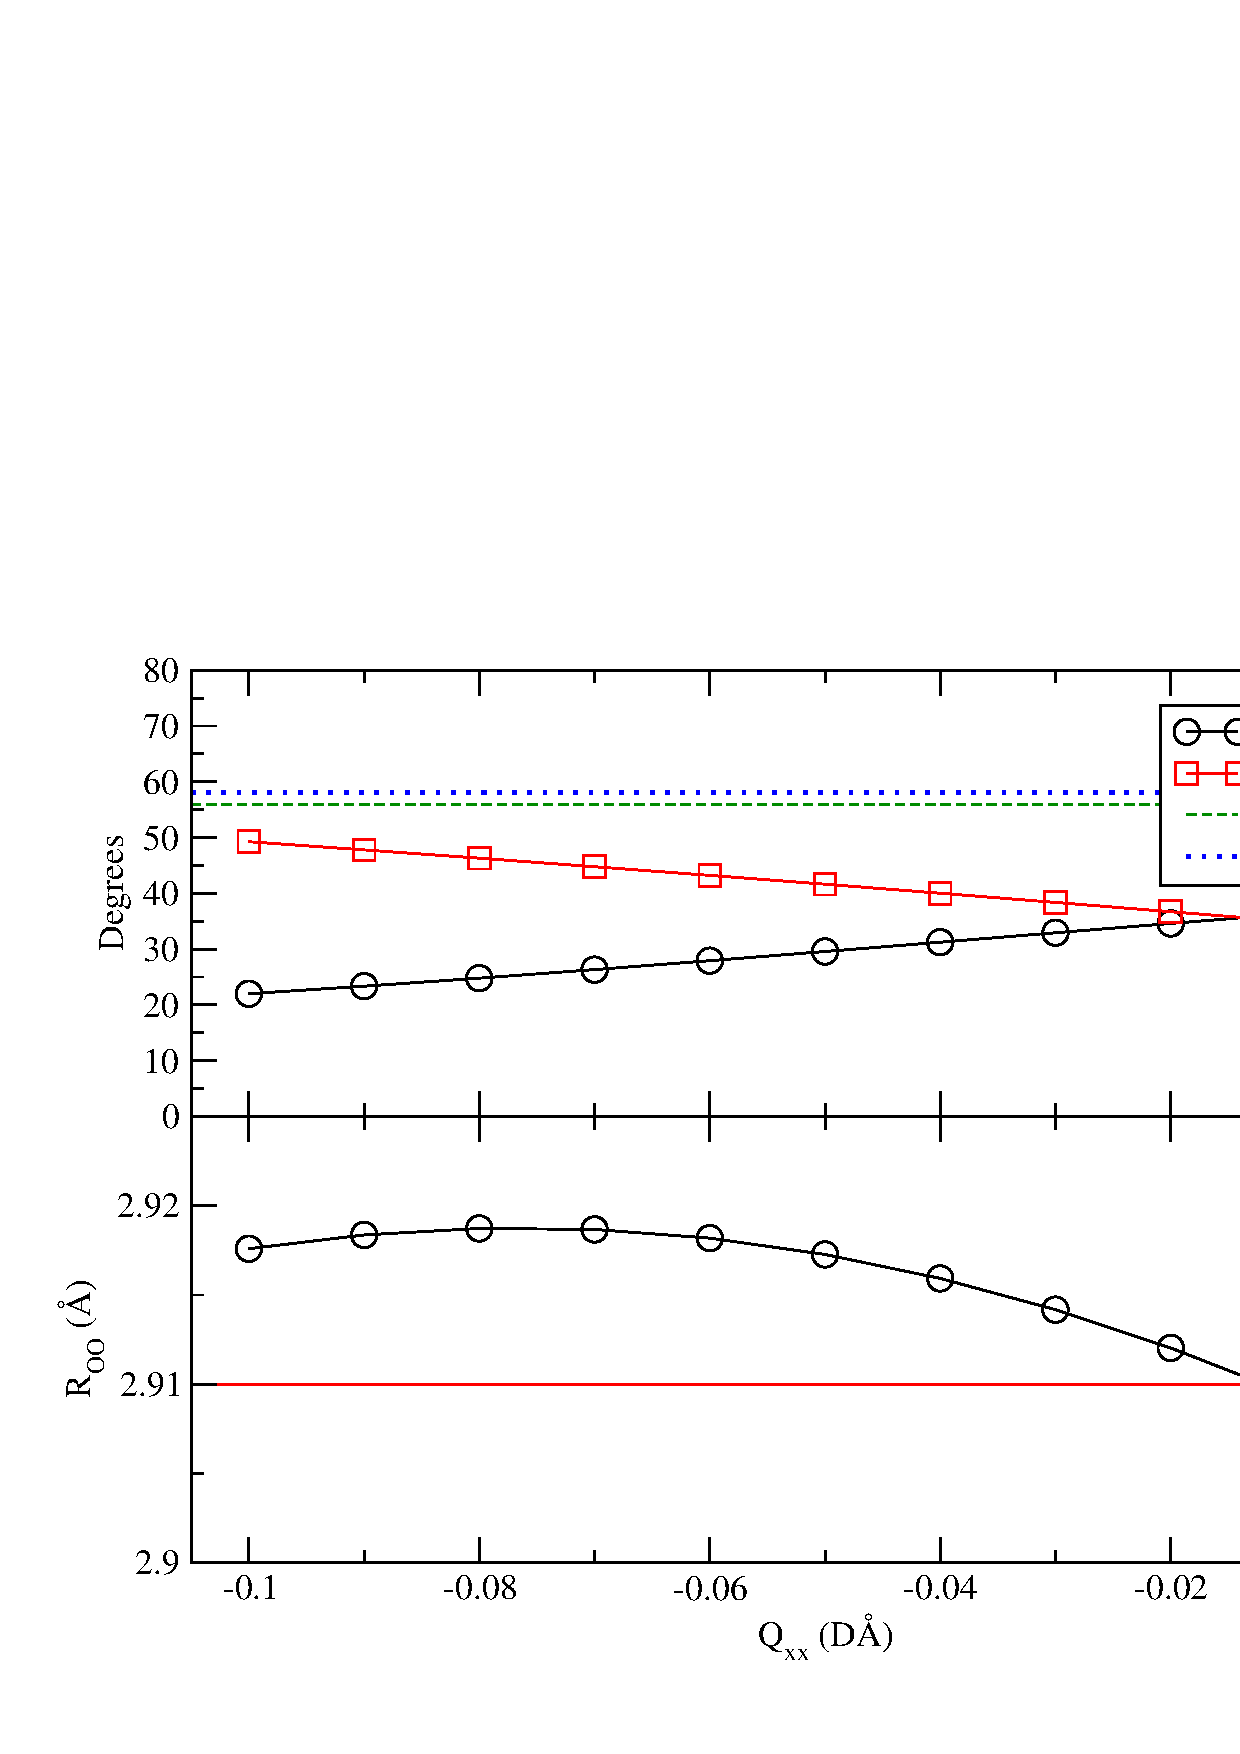
\includegraphics[width = \linewidth]{Figures/Test7_plot.pdf}
\caption{\label{fig:Qxx5} Setting $\sigma$ to 3.2268 \AA~, vary Q$_{xx}$ while simultaneously adjusting Q$_{yy}$ and Q${zz}$ to conserve Q$_T$ and $TrQ$.}
\end{figure}

It appears that we have achieved as close to the ab initio predicted values
as possbile without changing some of our fundamental assumptions. From Figure
\ref{fig:Qxx5}, I believe that by scaling the quadrupole and dipole by 
the same constant, thus keeping their ratio the same, we may be able to achieve
closer agreement with the ab initio predictions. While Abascal and Vega believe
that the largest value of Q$_T$ that will give reasonable T$_m$ for ice I$_h$
to be approximately 2.56 D\AA~, this prediction is made from water models which
contain point charges located on the Hydrogens. These charges cause a torque
on the other water molecule in the dimer structure, resulting in a change of
the magnitude of the angles.

In the following Test, Q$_{xx}$ was varied while simultaneously varying
Q$_{yy}$ to conserve the value of Q$_T$. 
$\mu$ was also scaled by $\mu = 0.996 Q_T$ for each Q$_T$ investigated. 
The $TrQ$ was set to 2.365707 D\AA~, and $\sigma$
was set to 3.2268 \AA~. In Figure \ref{fig:Q_T},R$_{OO}$, $\theta$, and 
$\phi$ are shown as Q$_{xx}$ and Q$_{yy}$ are varied.

\begin{figure}[h!]
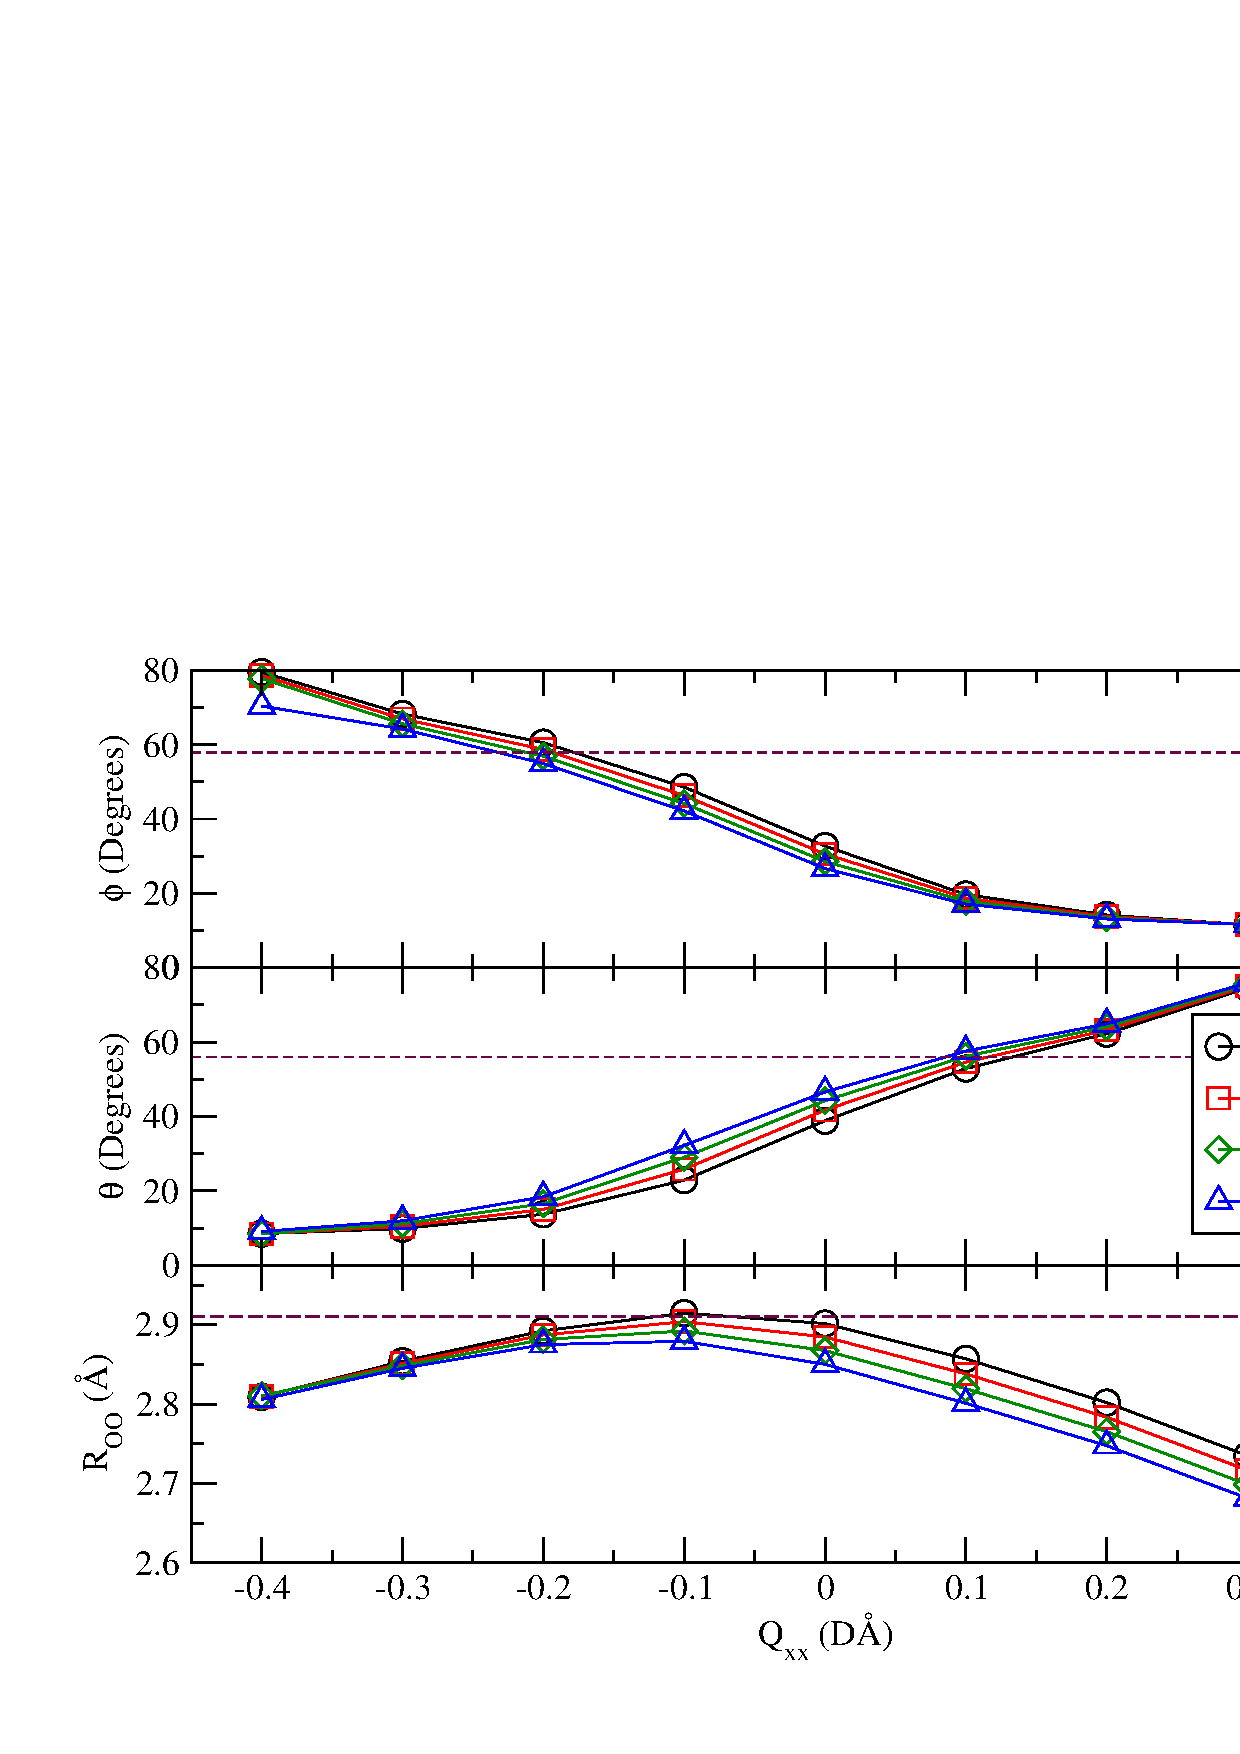
\includegraphics[width=\linewidth]{Figures/Test12_plot.pdf}
\caption{\label{fig:Q_T}Here Q$_{xx}$ and Q$_{yy}$ are varied simulatneously to conserve the value of Q$_T$. $\mu$ is scaled as $0.996 Q_T$, thus the ratio of $\mu$ to Q$_T$ is conserved for each Test of Q$_T$. The $TrQ$ is fixed to a set value, thus Q$_{zz}$ varies as the other components do. }
\end{figure}


In the next Test, the dipole moment of the model was varied by some scalar
amount ($\lambda$), relative to the Q$_T$ chosen. The Q$_{xx}$ component
of the quadrupole tensor was set to null, so Q$_{yy}$ varied for each 
case of Q$_T$. Q$_{zz}$ was fixed to the TIP1P/Ice model's value. The
results of this test can be seen in Figure \ref{fig:mew}.

\begin{figure}[h!]
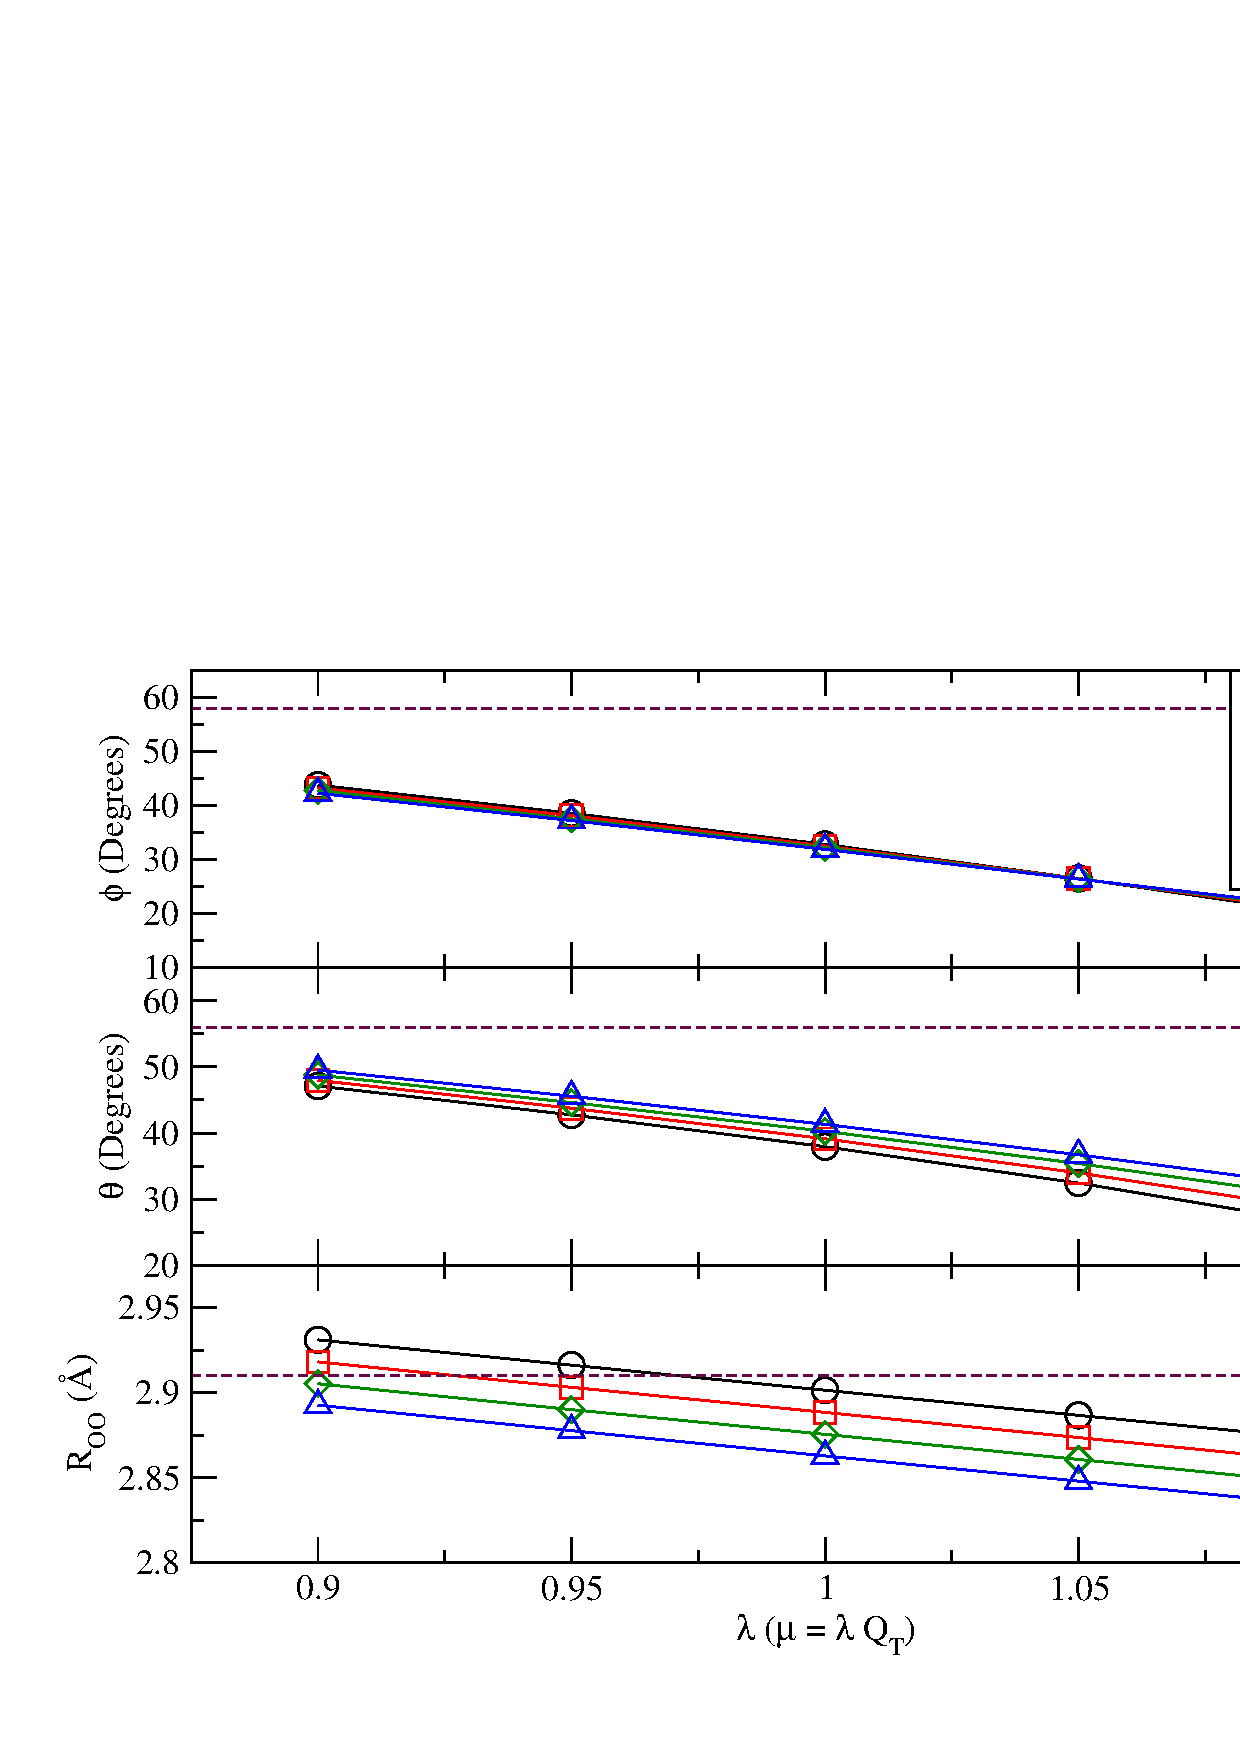
\includegraphics[width=\linewidth]{Figures/Test16_plot.pdf}
\caption{\label{fig:mew} }
\end{figure}
In the next section, I will construct a water model similar to the TIP1P/Ice 
model, however, it will not be the result of collapsing a many-site model onto
a single-site. This model will be derived from the results shown in this 
section with a larger dipole and quadrupole, in attempts to increase the 
magnitude of both of the angles without obscuring their ordering or the 
R$_{OO}$ values obtained above.

\subsection{TIP1P/Ice 2.0}

%The starting parameters for this section will be as follows: $\sigma = 3.2268$
%\AA~, $\mu = 2.56$ D, Q$_T = 2.56$, and the rest of the parameters are set to 
%the previous values.

%In Test 1, we will vary Q$_{xx}$ and Q$_{yy}$ while holding Q$_T$ constant. 
%Q$_{zz}$ is chosen to be a constant 0.73 D \AA~, thus the $TrQ$ will vary 
%throughout Test 1. In Figure \ref{fig:Qxx6}, R$_{OO}$ does not achieve the 
%ab initio predicted value of 2.91 \AA~, though comes closest at Q$_{xx}$
%values of about -0.3 D\AA~. 

%\begin{figure}[h!]
%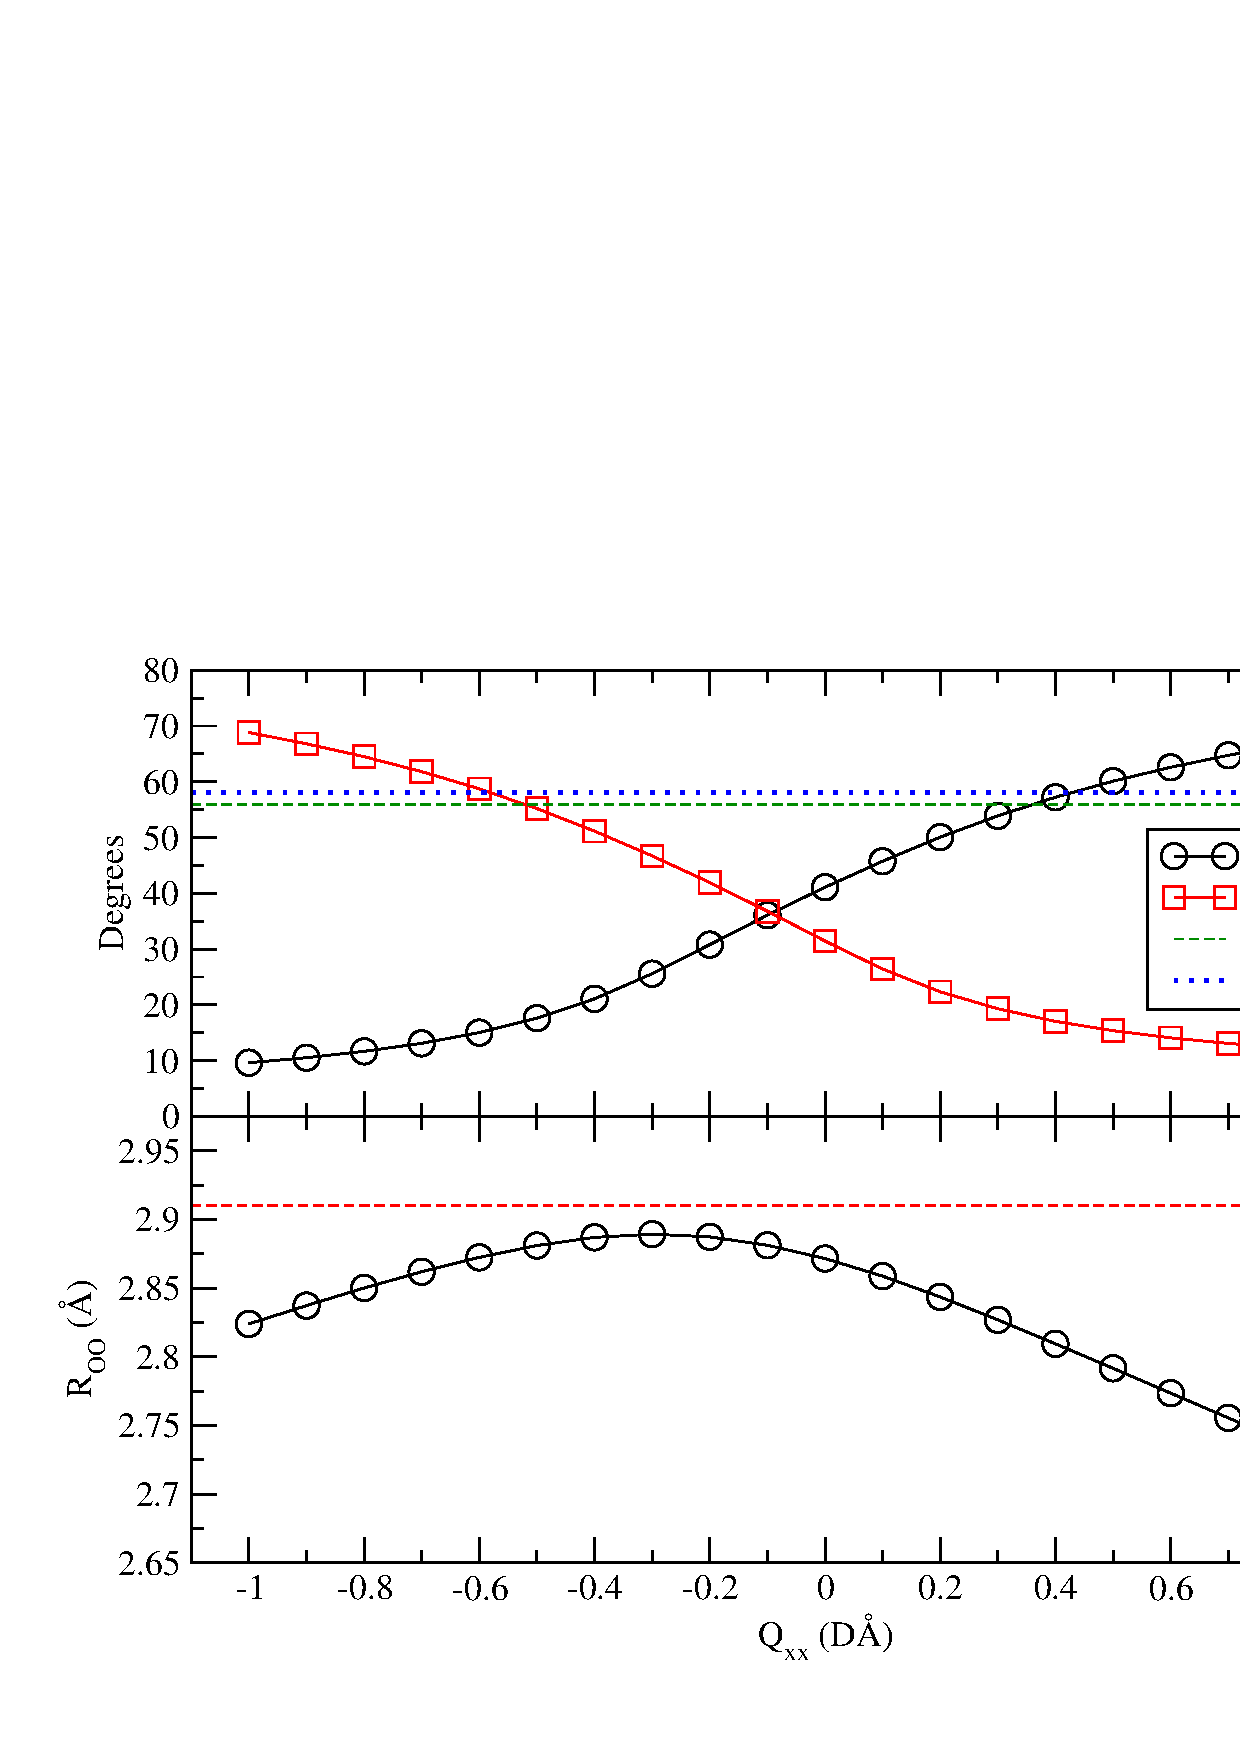
\includegraphics[width = 0.5\textwidth]{Test8_plot.pdf}
%\caption{\label{fig:Qxx6}Q$_{xx}$ is varied while simultaneously adjusting Q$_{yy}$ so that Q$_T$ is conserved. Q$_{zz}$ is not varied here, so the $TrQ$ changes as Q$_{xx}$ changes.}
%\end{figure}

In this section, we will worry less about holding Q$_T$ constant, and instead
hold QBar constant. In Figure \ref{fig:Qyy}, we have the results of varying
Q$_{yy}$ while holding Q$_{xx}$ constant at 0.1 D\AA~, and varying Q$_{zz}$
such that QBar fixed at the TIP4P/Ice value. However, we see that we do
not recover the TIP4P/Ice water dimer geometry.

\begin{figure}[h!]
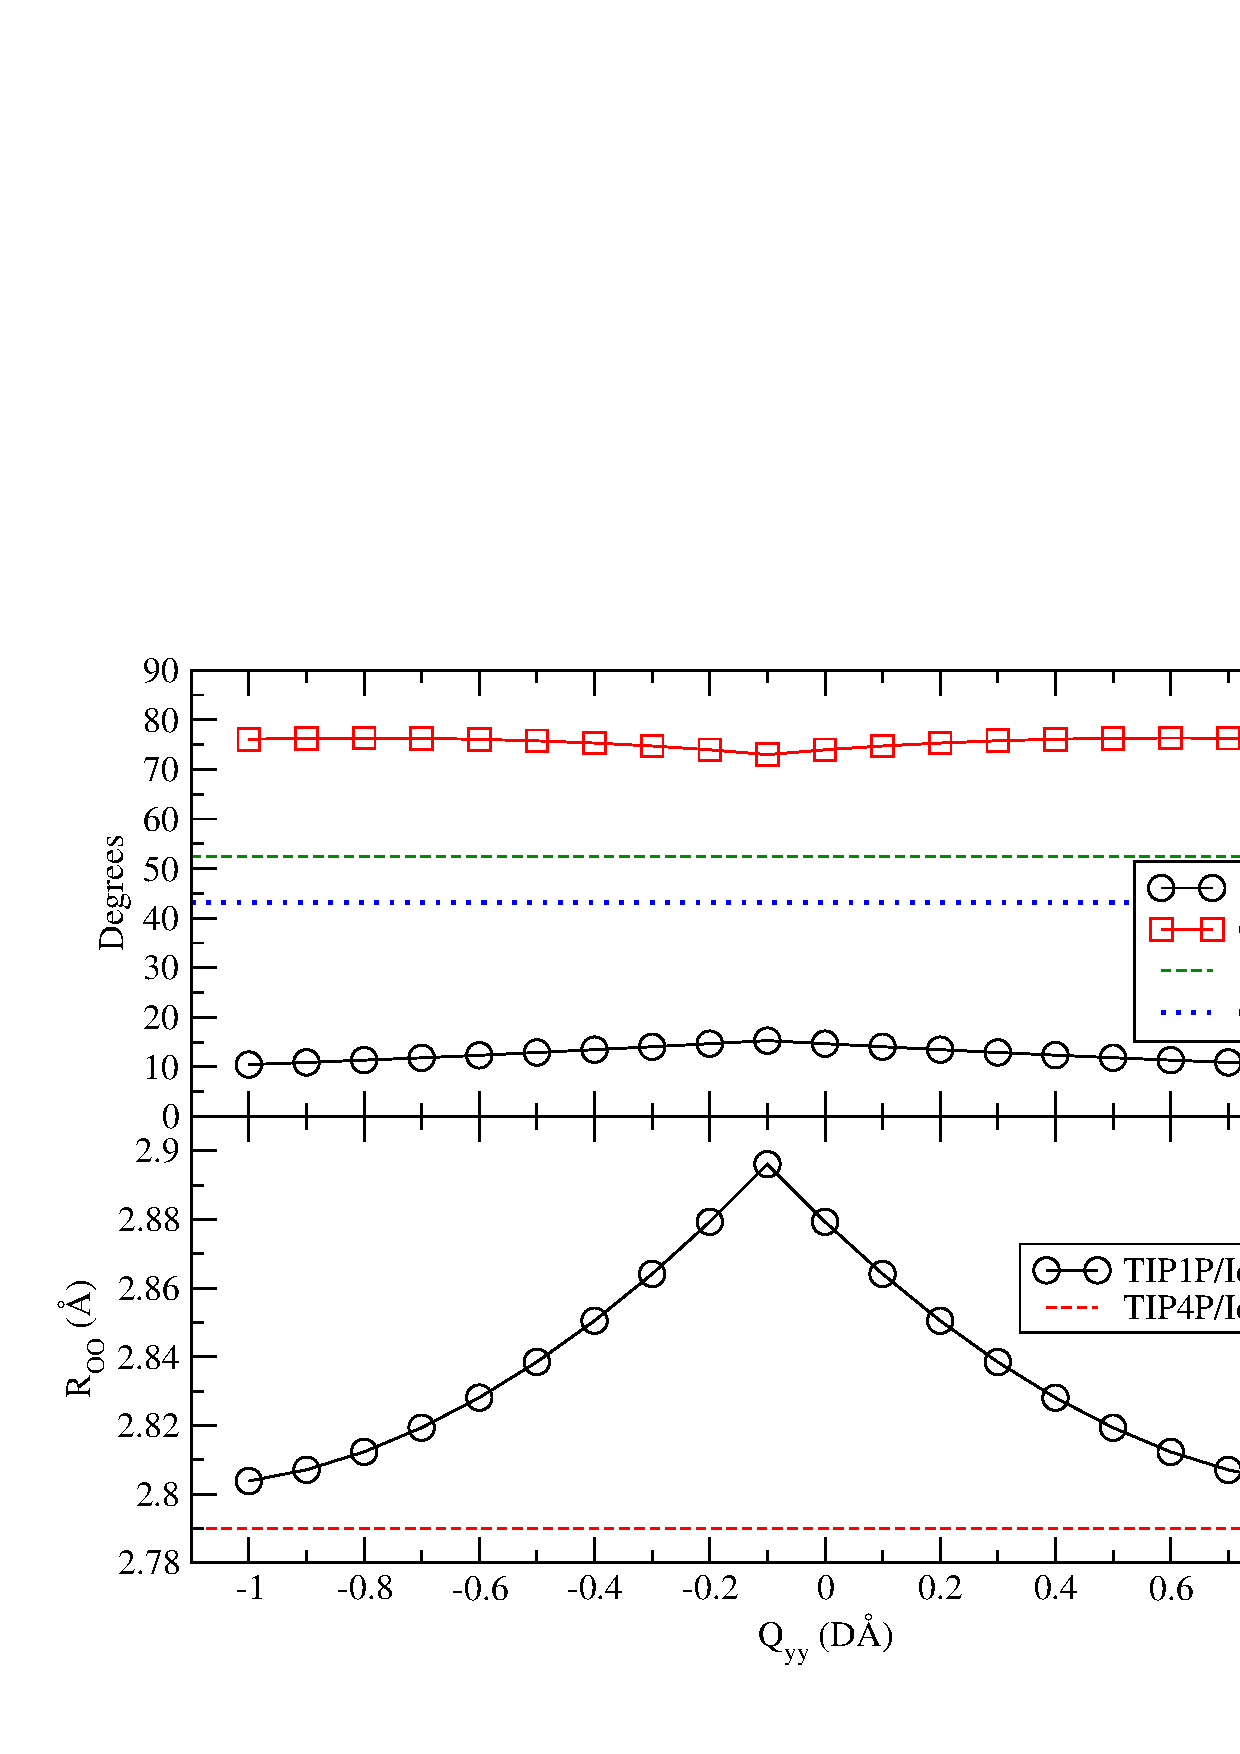
\includegraphics[width=\linewidth]{Figures/Test19_plot.pdf}
\caption{\label{fig:Qyy} Q$_{xx} = -0.1$, QBar set to the TIP4P/Ice QBar value of $2.8141$, Q$_{zz}$ was modified to keep this constant as Q$_{yy}$ changed.}
\end{figure}

It is interesting to note that the value of $\phi$ in Figure \ref{fig:Qyy} is 
much greater than initially expected from Figure \ref{fig:Qxx}. There, we would
predict $\phi \approx 40$ degrees, while here we have obtained a value of about
$76$ degrees. Also, there does not appear to be any appreciable change in the
values of $\theta$ as we vary Q$_{yy}$. This makes me wonder what controls
the value of $\theta$, as it appears to not be the value of Q$_{yy}$ as 
initially thought. In Figure \ref{fig:Qyy2}, we have held Q$_{yy}$ constant
at -0.1 D\AA~, and varied Q$_{xx}$ to see if it controls both $\phi$ and
$\theta$.

\begin{figure}[h!]
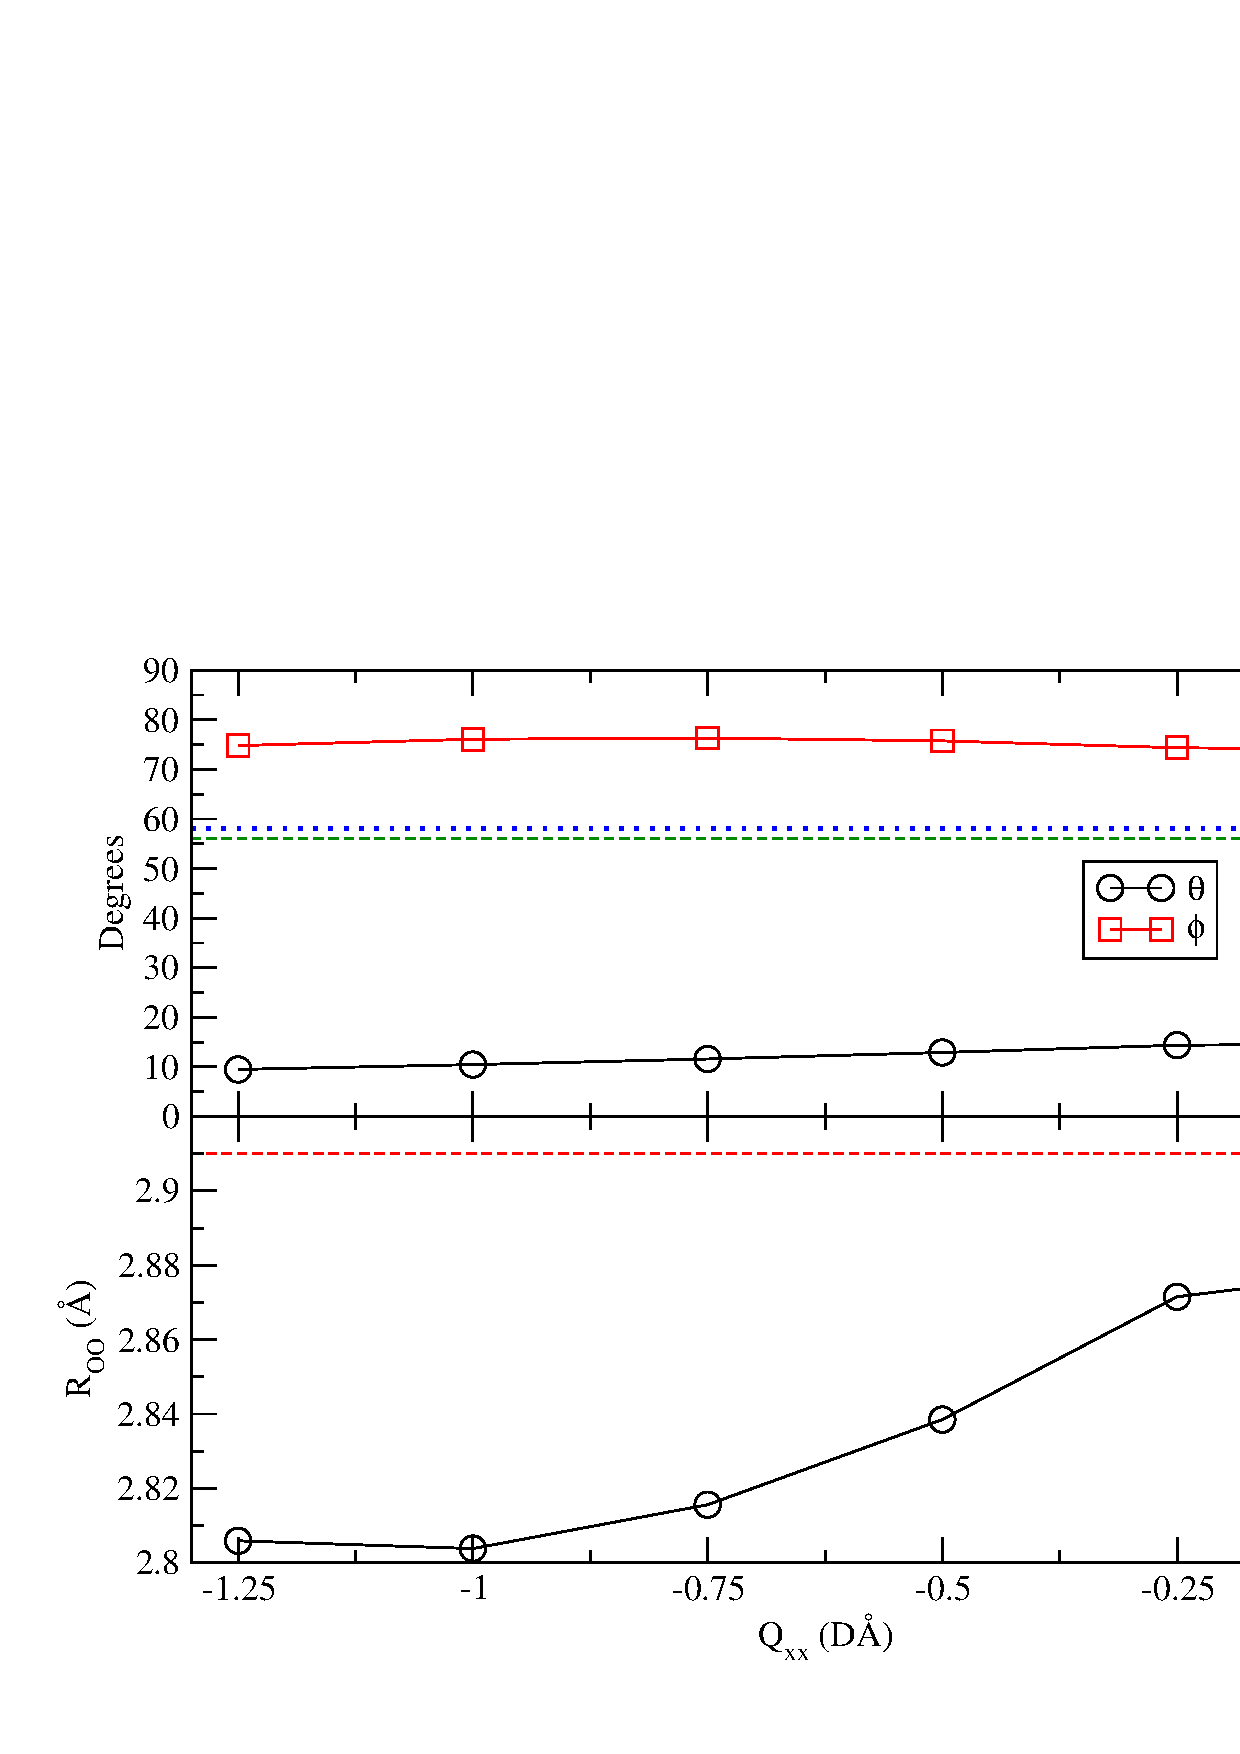
\includegraphics[width=\linewidth]{Figures/Test20_plot.pdf}
\caption{\label{fig:Qyy2} Q$_{yy} = -0.1$, Q$_{zz}$ was varied to keep QBar constant and equal to the TIP4P/Ice model's value of 2.8141.}
\end{figure}

From Figure \ref{fig:Qyy2}, we see that while R$_{OO}$ is slightly sensative
to the value of Q$_{xx}$, the angles $\theta$ and $\phi$ are both insensative
to it. In order to try and understand if and how the angles are dependent
on QBar, I have re-plotted the data from Figure \ref{fig:Qxx3} as a function
of QBar instead of Q$_{xx}$. This can be seen in Figure \ref{fig:QBar2}.

\begin{figure}[h!]
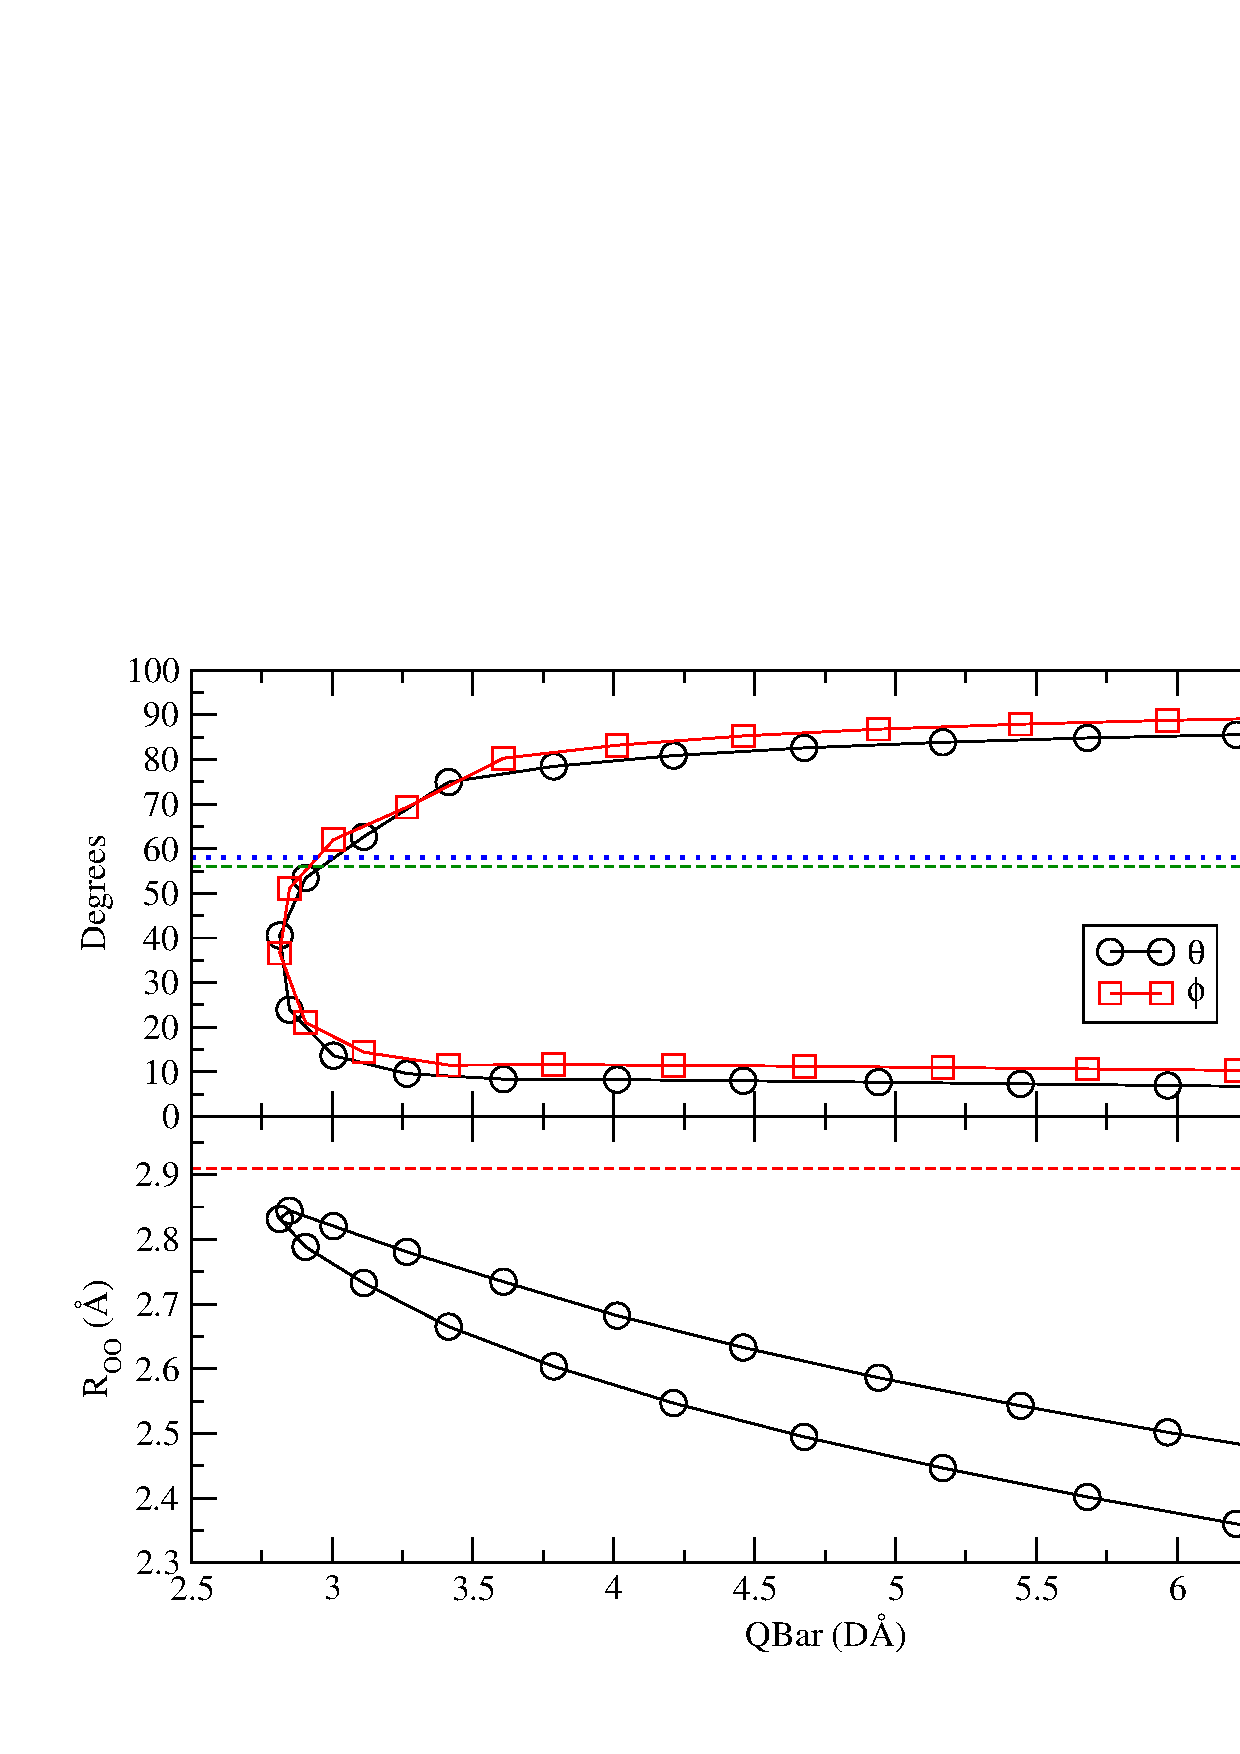
\includegraphics[width=\linewidth]{Figures/Test5_plot2.pdf}
\caption{\label{fig:QBar2}Q$_{xx}$ and Q$_{yy}$ varied while holding Q$_T$ constant, Q$_{zz}$ varied in order to keep $TrQ$ constant. Both Q$_T$ and $TrQ$ were set to the TIP4P/Ice model value.}
\end{figure} 

An interesting follow up test will be 
to set Q$_{xx}$ and Q$_{yy}$ to -0.1, Q$_{zz}$ to 1.3071, and vary $\mu$ to 
see if the desired angles can be achieved with a smaller dipole moment. The
results of doing so are shown in Figure \ref{fig:mu2}.

\begin{figure}[h!]
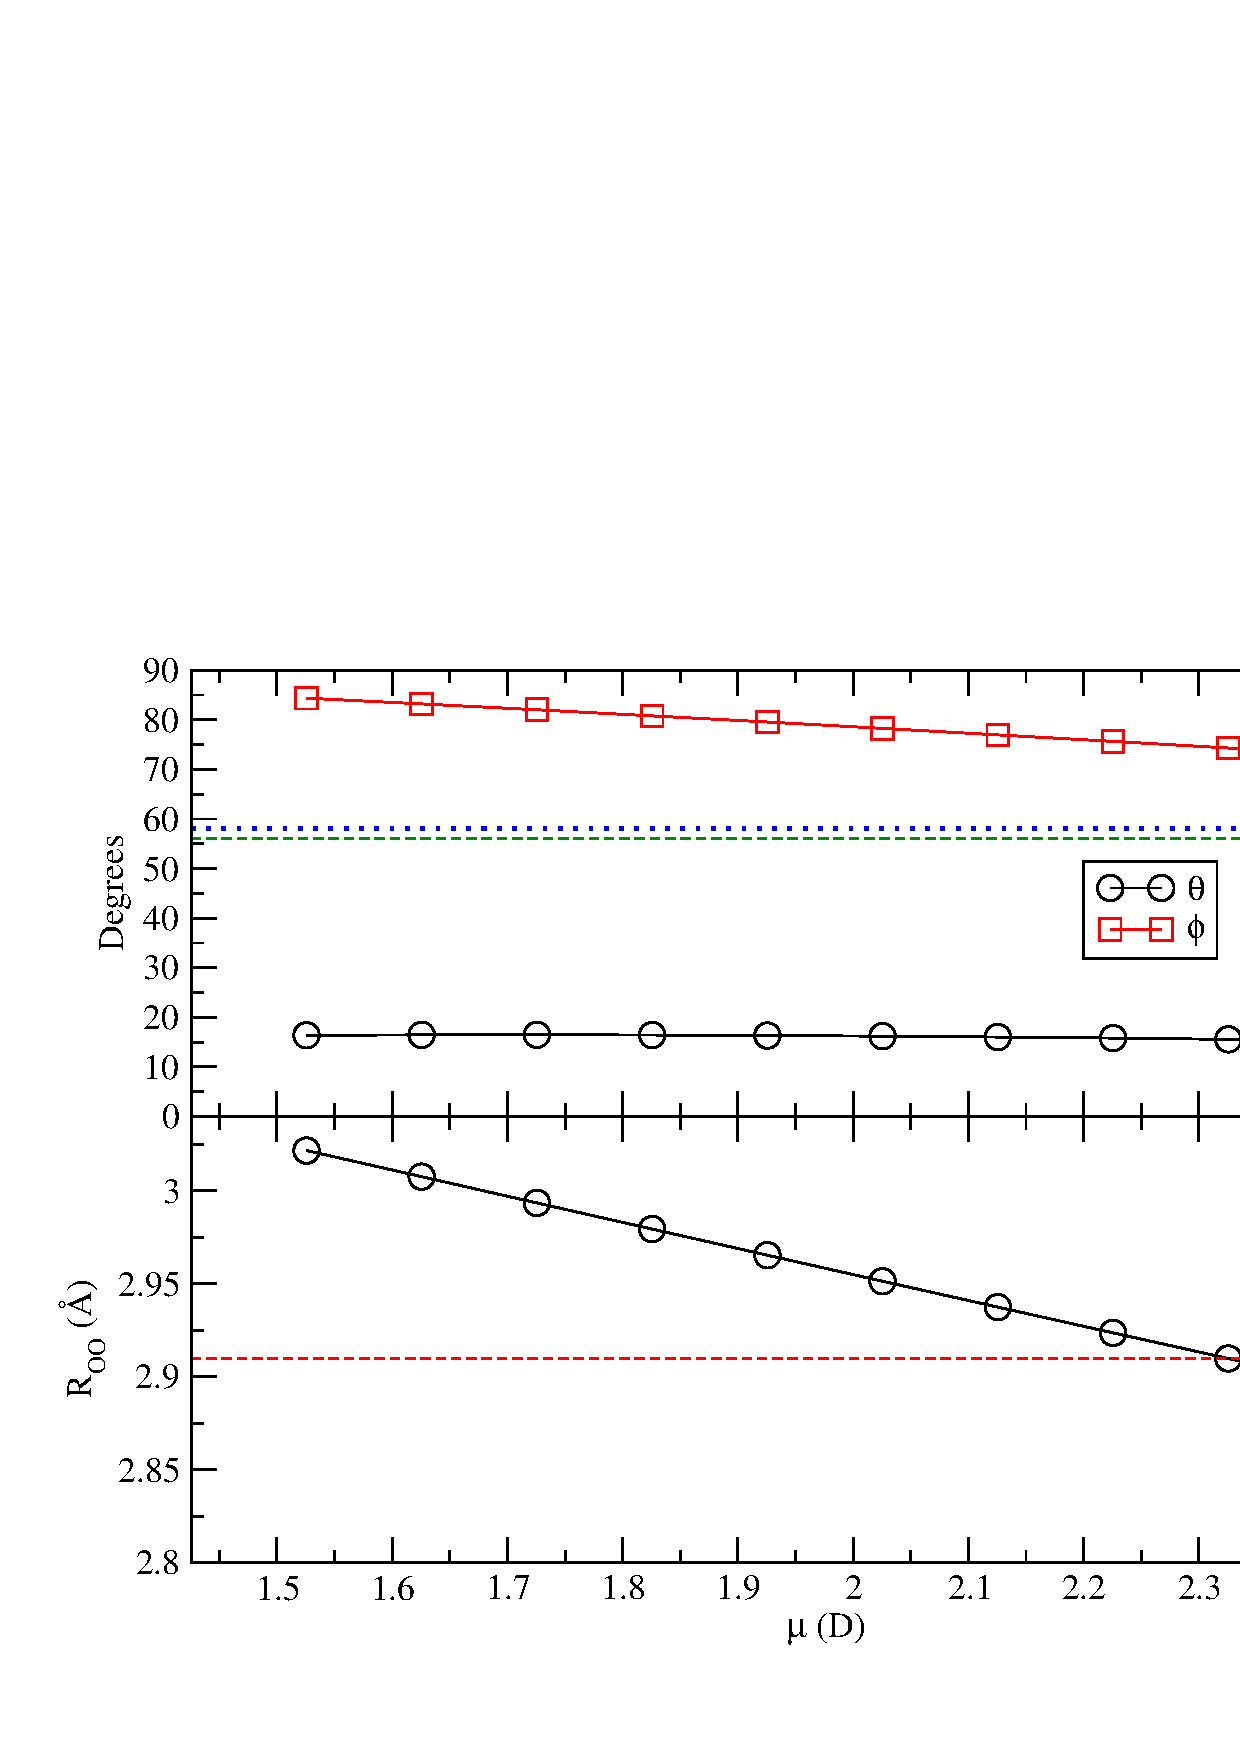
\includegraphics[width=\linewidth]{Figures/Test22_plot.pdf}
\caption{\label{fig:mu2} Q$_{xx} = -0.1$, Q$_{yy} = -0.1$, Q$_{zz} = 1.3701$ which ensures QBar is set to the TIP4P/Ice model value of $2.8141$ D\AA~.}
\end{figure}

In Figure \ref{fig:mu2}, we see that as we decrease the value of the dipole 
moment, the water dimer's separation distance, R$_{OO}$ gradually becomes 
larger. The angle $\phi$ increases slightly with decreasing $\mu$, however, 
$\theta$ is relatively insensitive to the value of $\mu$.
 
In the next Test, we have set the Lennard-Jones parameters to that of the
TIP4P/Ice model, as well as the Q$_{xx}$ and Q${zz}$ values. Q$_{yy}$ is 
allowed to vary, and as such, Q$_T$ and QBar both vary. In Figure
\ref{fig:Qyy3}, we see that the angle $\theta$ is obtained when Q$_{yy}$
is set to about 1.87 D\AA~. However, we see that we miss the dimer 
separation distance at this value of Q$_{yy}$, as well as the angle
$\phi$, which we believe to be the less important of the two angles.

\begin{figure}[h!]
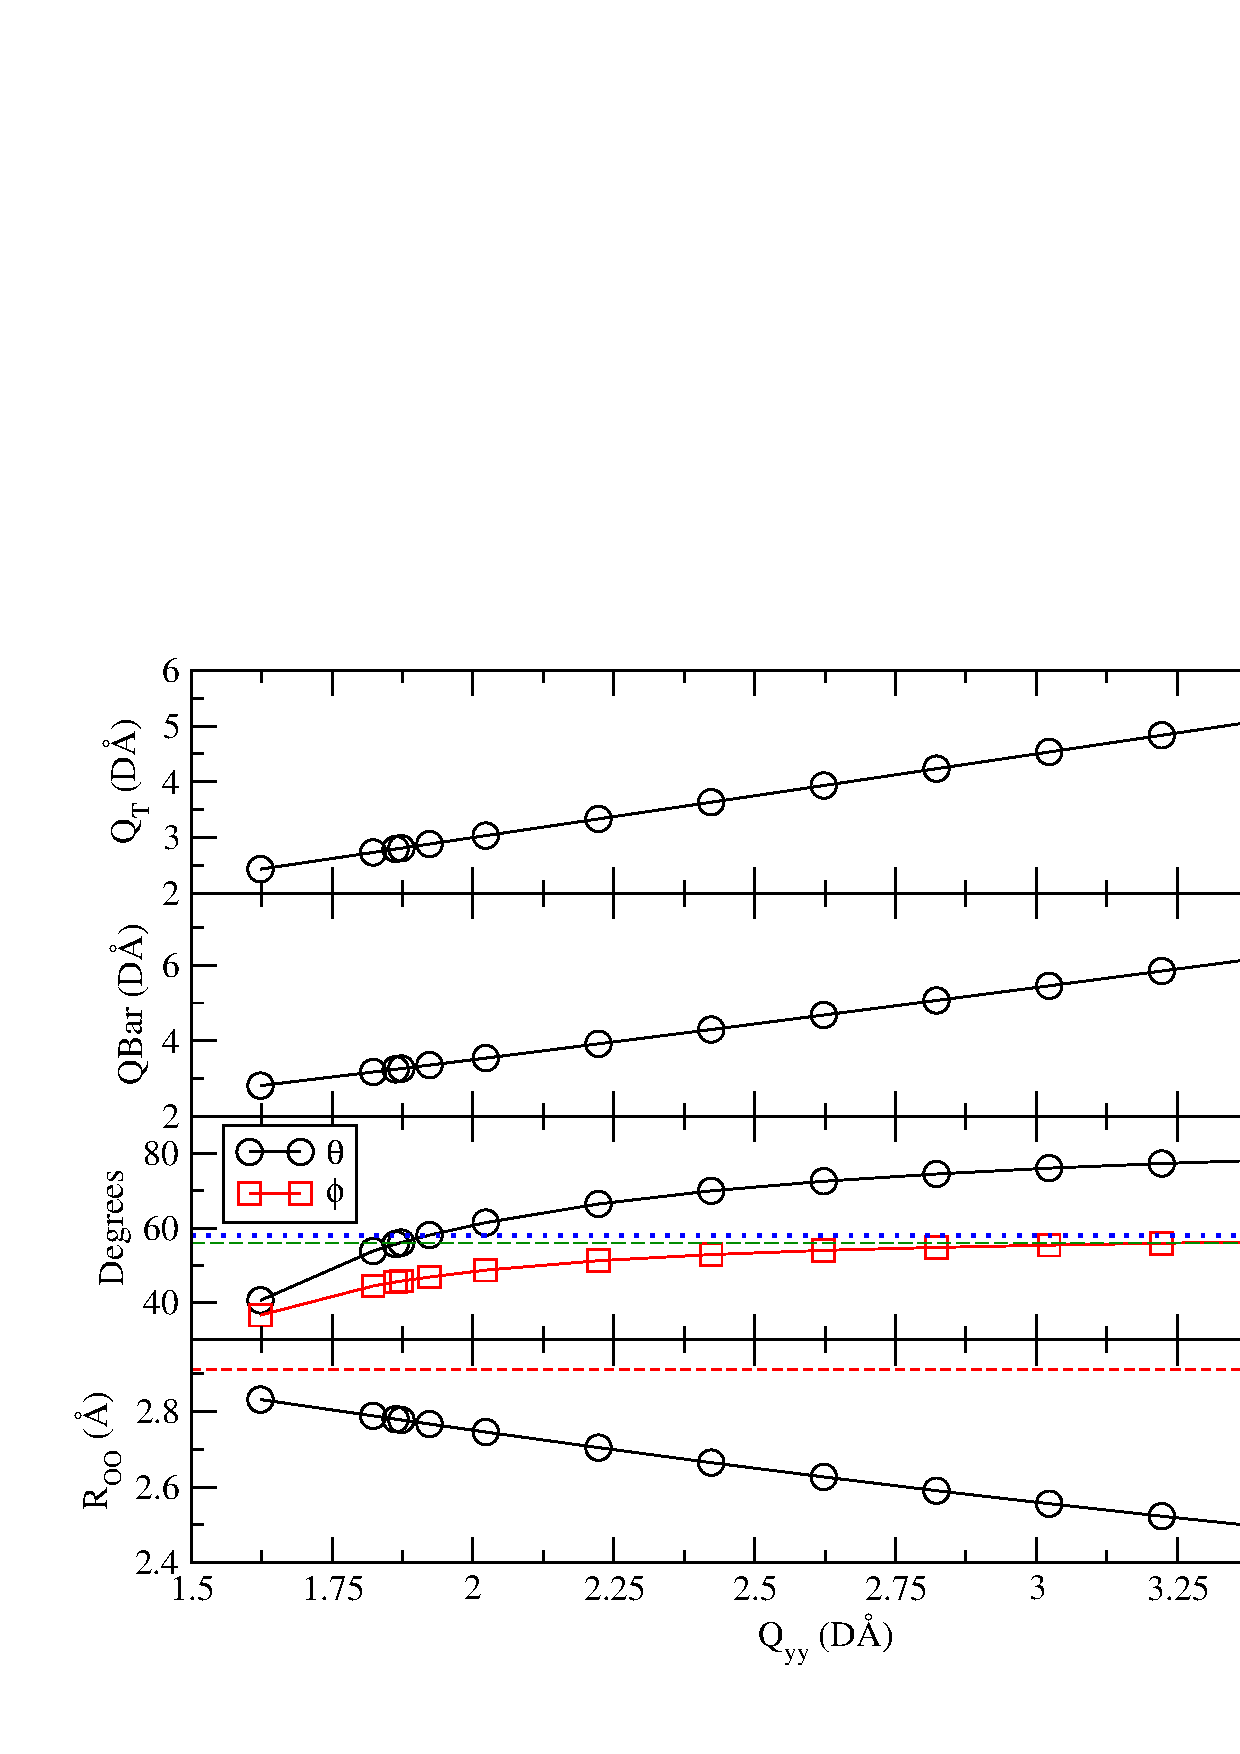
\includegraphics[width=\linewidth]{Figures/Test23_plot.pdf}
\caption{\label{fig:Qyy3} Q$_{xx}$ and Q$_{zz}$ are set to the TIP4P/Ice value, as well as the Lennard-Jones parameters.The left most data point is the parameter set of the TIP4P/Ice model.}
\end{figure}

In a similar way, we have held Q$_{yy}$ and Q$_{zz}$ constant while varying
Q$_{xx}$. The results of doing so can be seen in Figure \ref{fig:Qyy4}.

\begin{figure}[h!]
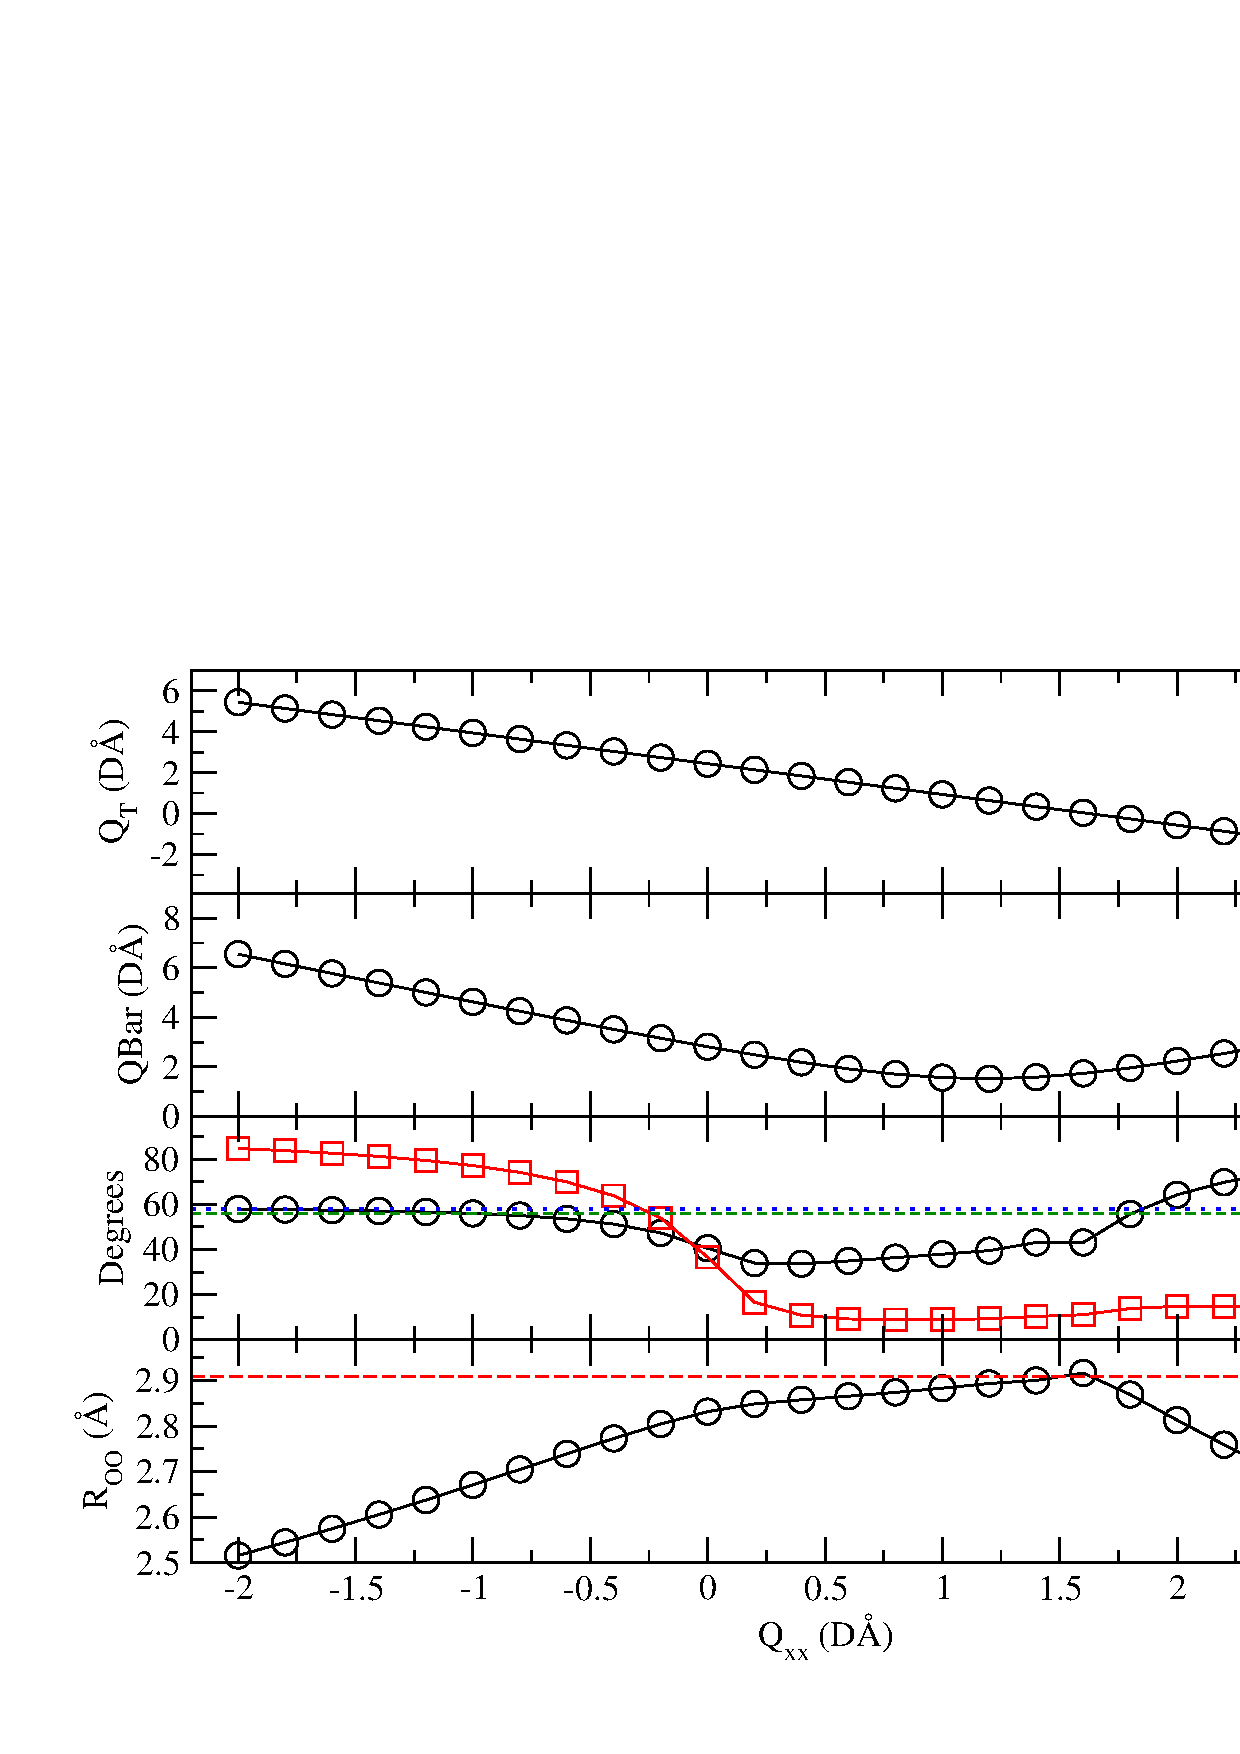
\includegraphics[width=\linewidth]{Figures/Test24_plot.pdf}
\caption{\label{fig:Qyy4} Q$_{yy}$ and Q$_{zz}$ are set to the TIP4P/Ice value,as well as the Lennard-Jones parameters.The left most data point is the parameter set of the TIP4P/Ice model.}
\end{figure}

Finally, we have finished the permutation by varying Q$_{zz}$ while holding
Q$_{xx}$ and Q${yy}$ constant at their original TIP4P/Ice values, as seen
in Figure \ref{fig:Qyy5}.

\begin{figure}[h!]
\includegraphics[width=\linewidth]{Figures/Test25_plot.pdf}
\caption{\label{fig:Qyy5} Q$_{xx}$ and Q$_{yy}$ are set to the TIP4P/Ice value,\
as well as the Lennard-Jones parameters.The left most data point is the parameter set of the TIP4P/Ice model.}
\end{figure}


\subsection{Bulk Properties}
As an initial test of the bulk phase properties, I have equilibrated two
separate water boxes, one containing 1372 molecules, and one
containing 4000 molecules. The resulting geometry was a cubic
box with side length of 48.57617 \AA~. The molecules were propaged at 300K for
1 nanosecond, saving coordinates every 0.1 ps for analysis. The 
three-dimensional diffusion constant was found to be 
$5.488\times10^{-5}$cm$^{2}$s$^{-1}$. This is about a factor of two larger
than the experimentally reported value of 2.30 cm$^{2}$s$^{-1}$. We attribute
this difference to a lack of strength of hydrogen bonding. Due to this,
we will try playing with the dipole strength and the Q$_{zz}$ values.
		

\subsection{Basal Ice I$_{h}$/water Coexistence}
In order to tune the model to the desired observable, I have begun testing 
the model at the ice I$_{h}$/water interface, exposing a basal plane to bulk 
water. This system was prepared by constructing a large block of ice from 
crystallographic coordinates taken from Hirsch and Ojamae structure number
6\cite{Hirsch2004}. The constructed block is periodic in all three dimensions. 
The block was positioned in a simulation cell such that the basal face pointed
along the positive $z$-dimension. The ice block was allowed to relax and 
equilibrated to 75 K. Separately, a simulation box of liquid water with a 
density of 0.999 g cm$^{-1}$ was 
equilibrated to 75 K, with equivalent $x$ and $y$ dimensions to the ice block,
and twice that in $z$. The ice block was then merged with the liquid system
by carving out any liquid water molecule within three angstroms of a molecule
from the ice system.
	
%		\caption{\label{fig:RC} Comparison of ``Bragg Peak" location at 0.1 T and 0.2 T on the (111) symmetry axis.  It would appear that the Bragg peak is actually background fluctuations, and that the initial location at the correct $\vec{q}$ was an unfortunate coincidence.}
%	\end{figure}
	
%	\begin{figure}
%		\includegraphics[width=0.45\textwidth]{fwhm.pdf}
%		\caption{\label{fig:fwhm} Comparison of ``Bragg Peak" location at 0.1 T and 0.2 T on the (111) symmetry axis.  It would appear that the Bragg peak is actually background fluctuations, and that the initial location at the correct $\vec{q}$ was an unfortunate coincidence.}
%	\end{figure}

		
\chapter{ADDITIONAL STRUCTURAL PROFILES OF ICE-I$_\mathrm{h}$ / WATER INTERFACES}\label{structAppendix}

Contained in this appendix are additional tetrahedrality, thermal, and
velocity profiles of the TIP4P/Ice and SPC/E ice-I$_\mathrm{h}$
/ water interfaces.


\begin{figure*}
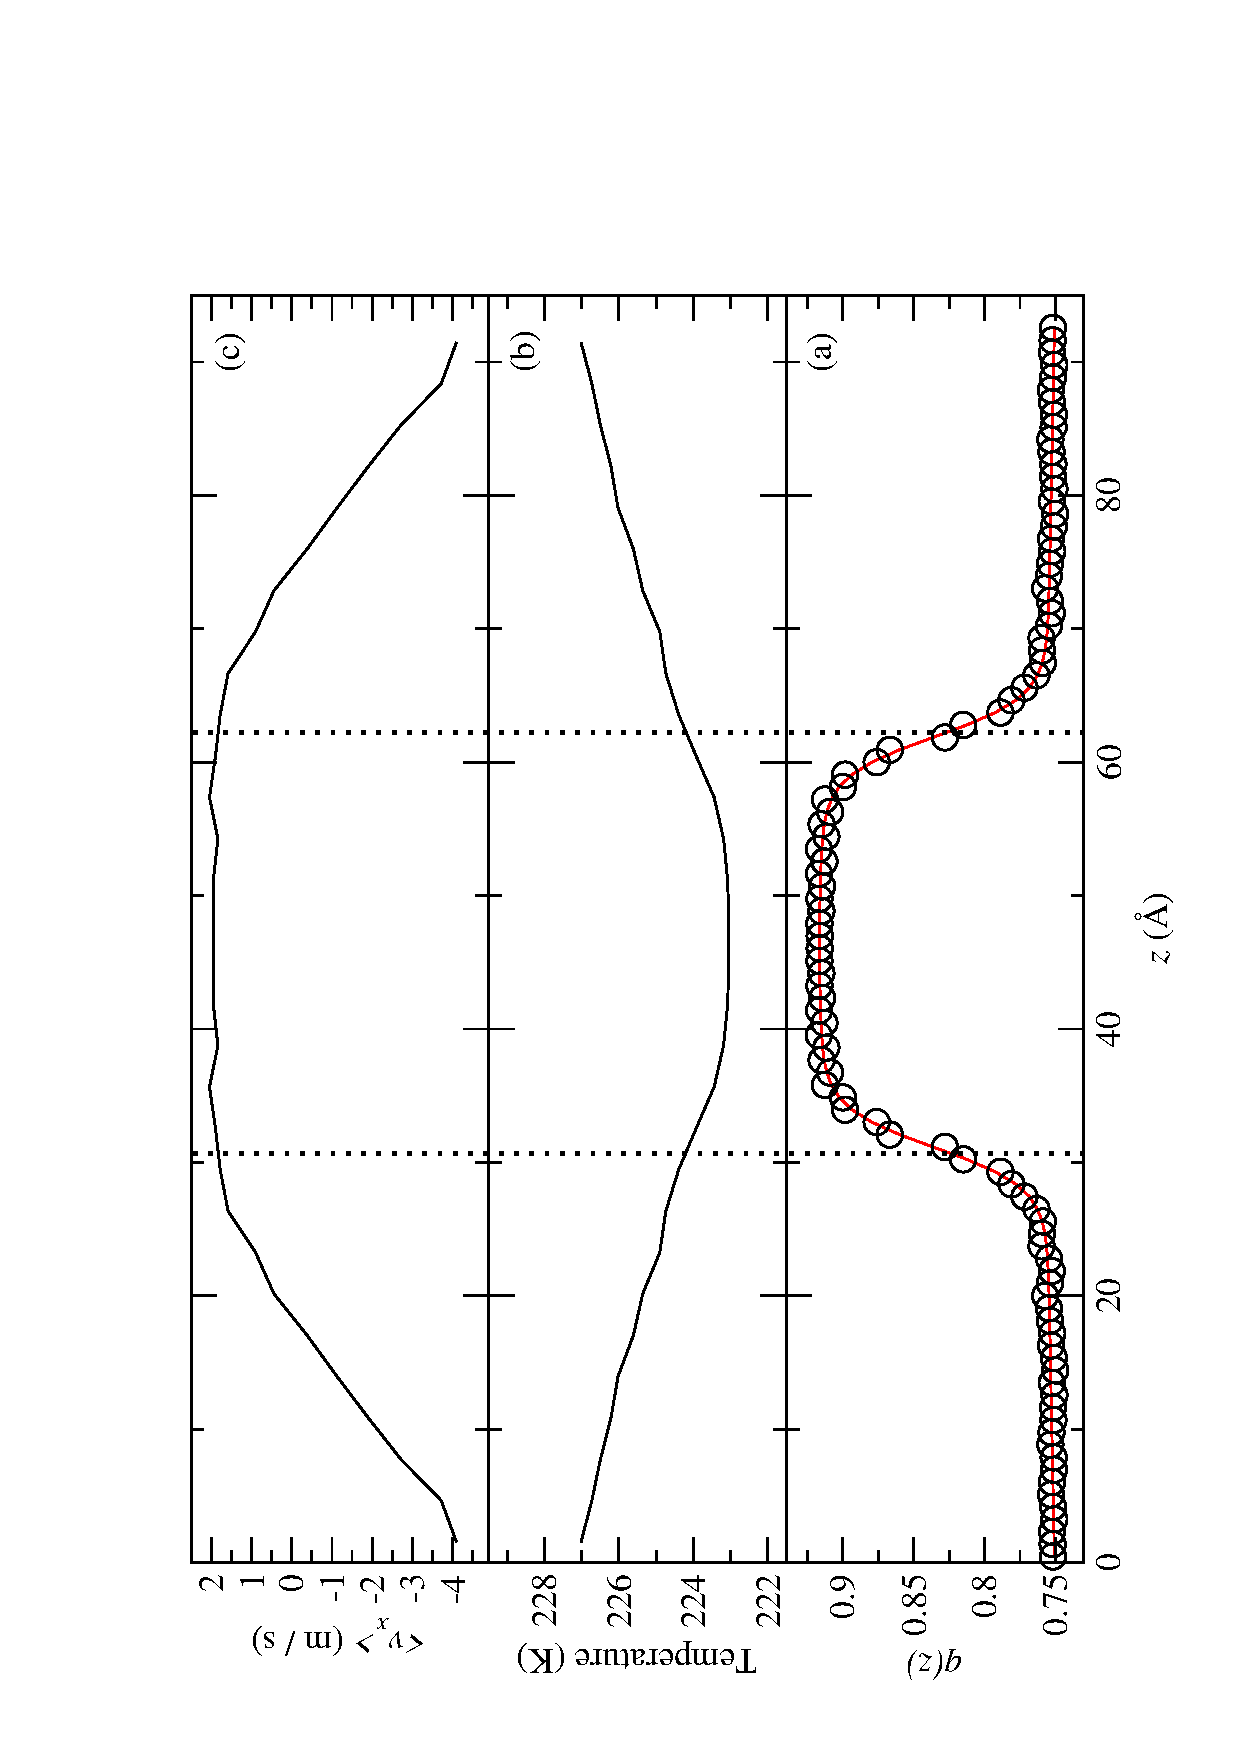
\includegraphics[width=\linewidth]{Figures/Pyr_comic_strip}
\caption{\label{fig:pyrComic} Properties of the SPC/E pyramidal
  interface being sheared through water at 7.6
  ms\textsuperscript{-1}. Lower panel: the local tetrahedral order
  parameter, $q(z)$, (circles) and the hyperbolic tangent fit
  (turquoise line).  Middle panel: the imposed thermal gradient
  required to maintain a fixed interfacial temperature of 225 K. Upper
  panel: the transverse velocity gradient (squares) that develops in
  response to an imposed momentum flux, along with the fit (green
  line). The vertical dotted lines indicate the locations of the Gibbs
  dividing surfaces of the two interfaces.}
\end{figure*}

\begin{figure*}
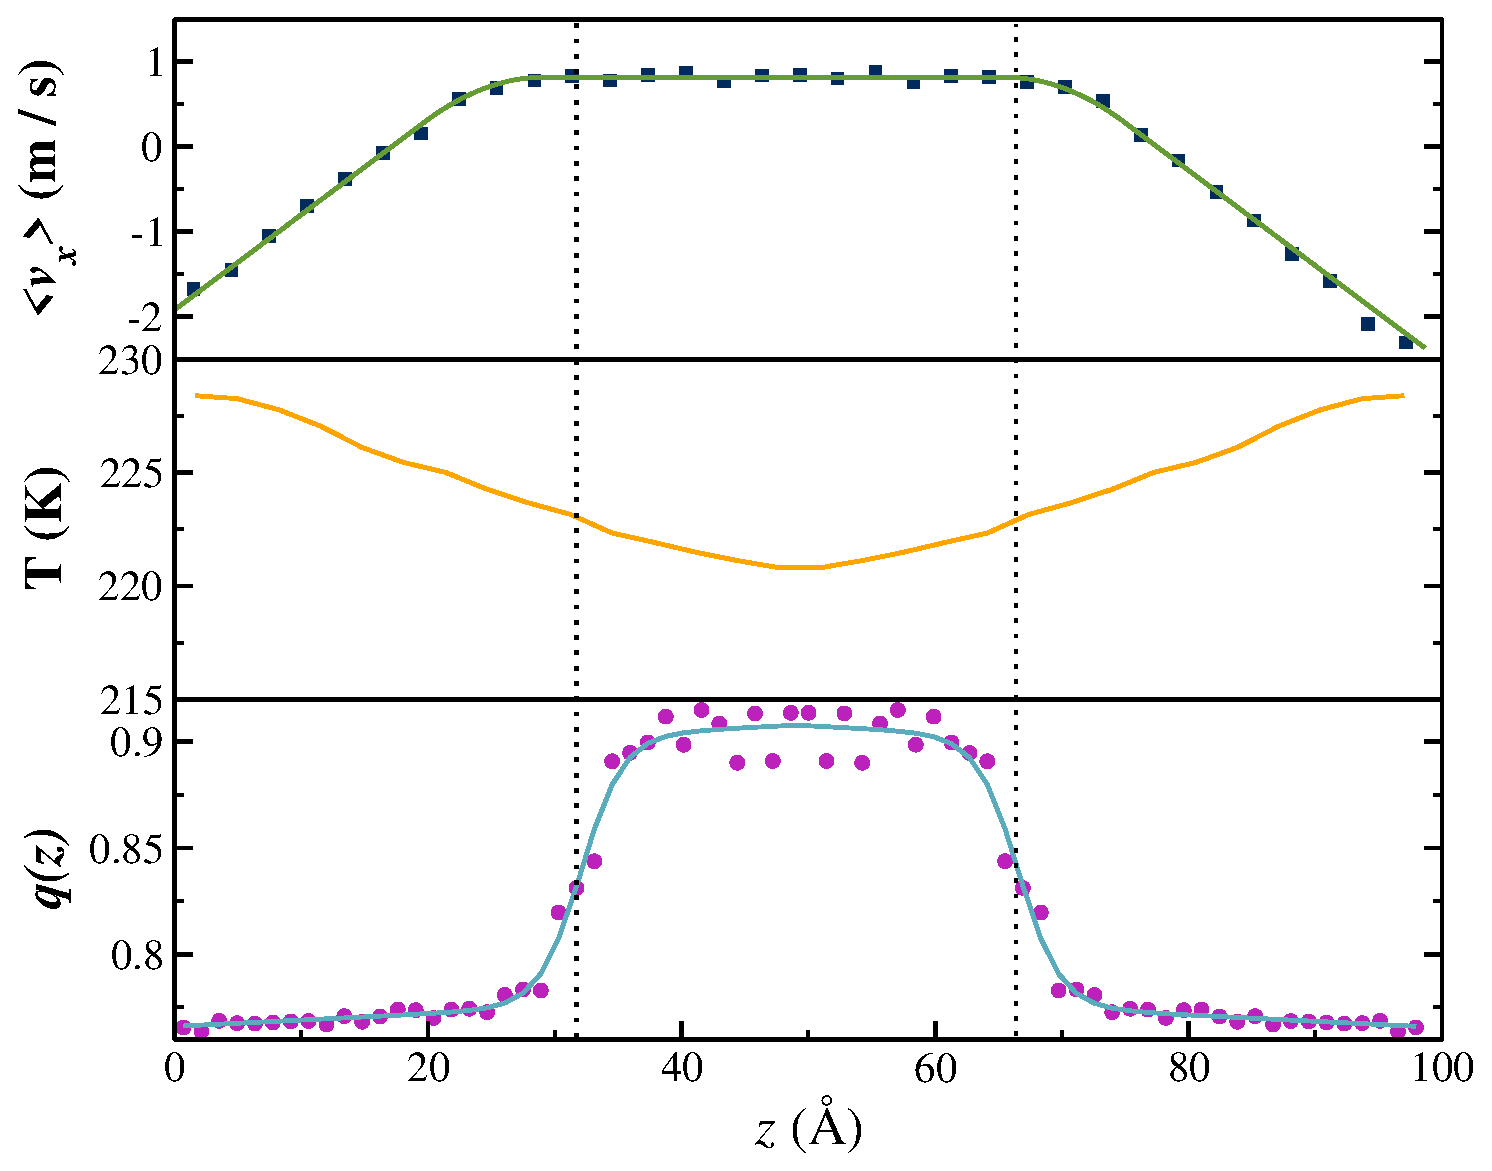
\includegraphics[width=\linewidth]{Figures/Bas_comic_strip}
\caption{\label{fig:bComic} Properties of the SPC/E basal interface being
  sheared through water at 3.2 ms\textsuperscript{-1}.  Panel
  descriptions are the same as in Fig. \ref{fig:pyrComic}.}
\end{figure*}

\begin{figure*}
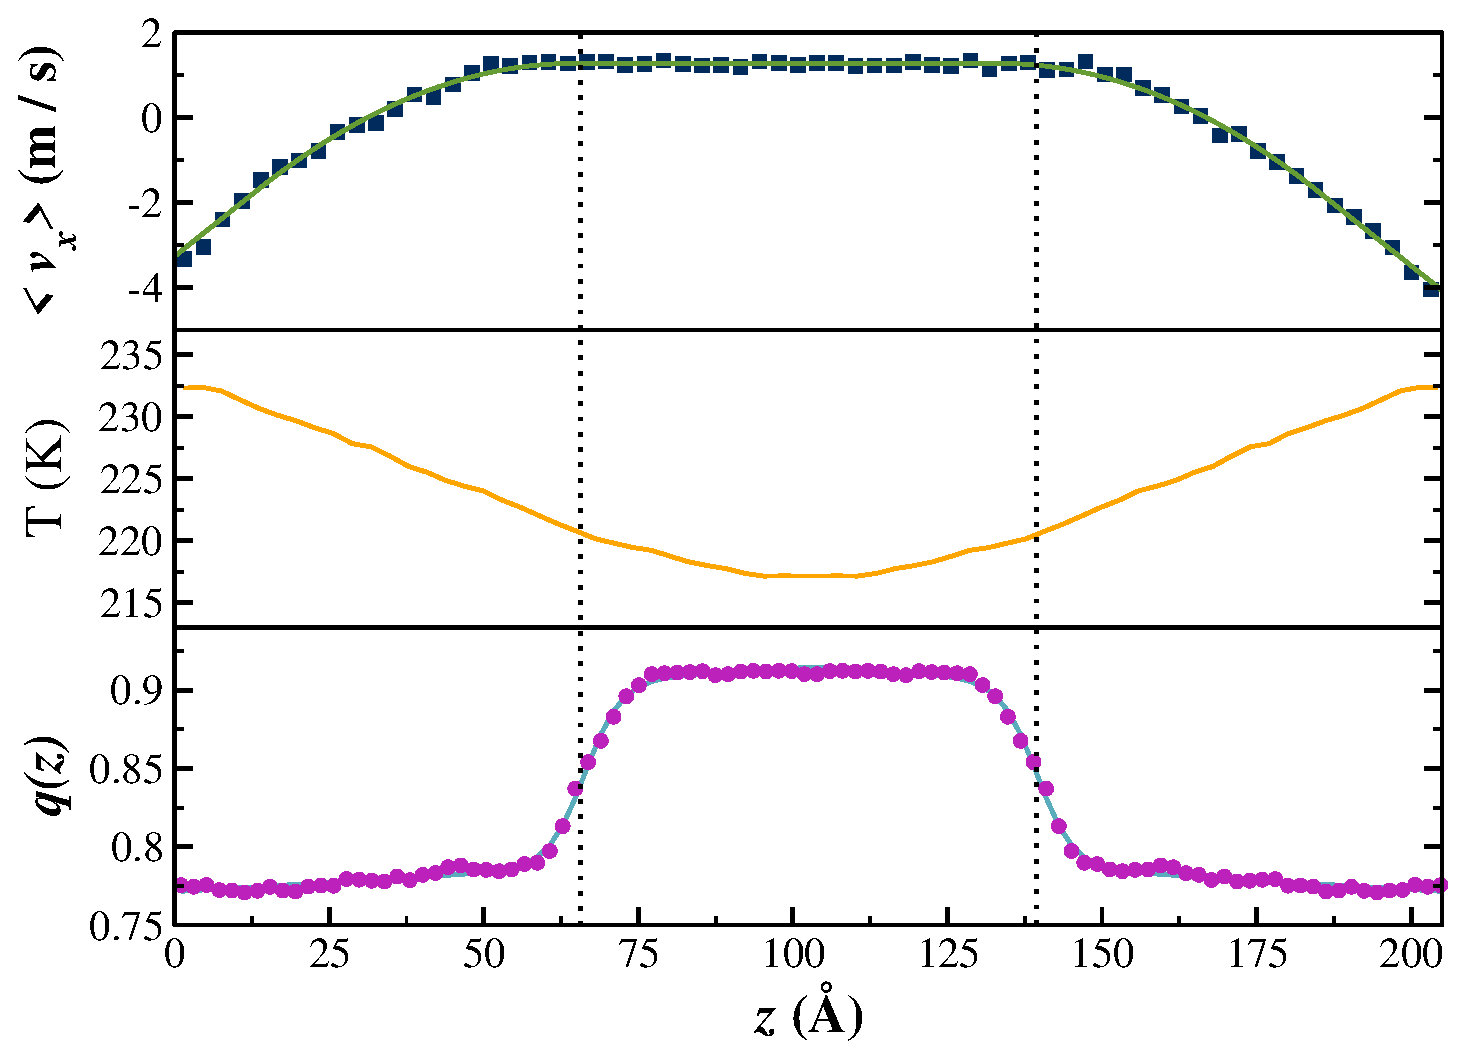
\includegraphics[width=\linewidth]{Figures/Pri_comic_strip}
\caption{\label{fig:pComic} Properties of the SPC/E prismatic interface
  being sheared through water at 6.0 ms\textsuperscript{-1}.  Panel
  descriptions are the same as in Fig. \ref{fig:pyrComic}.}
\end{figure*}

\begin{figure*}
\includegraphics[width=\linewidth]{Figures/Basal_TIP4PIce_Plot}
\caption{\label{fig:tipbComic} Properties of the TIP4P/Ice basal
  interface being sheared through water at 6.1
  ms\textsuperscript{-1}. Lower panel: the local tetrahedral order
  parameter, $q(z)$, (circles) and the hyperbolic tangent fit
  (blue line).  Middle panel: the imposed thermal gradient
  required to maintain a fixed interfacial temperature of 270 K. Upper
  panel: the transverse velocity gradient (squares) that develops in
  response to an imposed momentum flux, along with the fit (purple
  line). The vertical dotted lines indicate the locations of the Gibbs
  dividing surfaces of the two interfaces.}
\end{figure*}

\begin{figure*}
\includegraphics[width=\linewidth]{Figures/Prism_TIP4PIce_Plot}
\caption{\label{fig:tippComic} Properties of the TIP4P/Ice prismatic
  interface being sheared through water at 7.4 ms\textsuperscript{-1}.
  Panel descriptions are the same as in Fig. \ref{fig:tipbComic}.}
\end{figure*}

\begin{figure*}
\includegraphics[width=\linewidth]{Figures/Pyra_TIP4PIce_Plot}
\caption{\label{fig:tippyComic} Properties of the TIP4P/Ice prismatic
  interface being sheared through water at 8.1 ms\textsuperscript{-1}.
  Panel descriptions are the same as in Fig. \ref{fig:tipbComic}.}
\end{figure*}


\begin{figure*}
\includegraphics[width=\linewidth]{Figures/TIPtransDensity}
\caption{\label{fig:TIPtransDensity} Transverse density profiles for the
  basal (a), prismatic (b), 14\degree~pyramidal (c) and secondary prism (d)
  facets of an TIP4P-Ice ice-I$_\mathrm{h}$ / water interface (black
  lines). The prismatic and secondary prism profiles are zoomed in to
  show detail at the ice / water interface. The profiles are fit using
  Eq. \eqref{rho_fit} (dashed red lines). }
\end{figure*}
\chapter{ADDITIONAL REORIENTATIONAL DECAY PLOTS FOR ICE-I$_\mathrm{h}$ / WATER INTERFACES}\label{dynamicAppendix}

Contained in this appendix are additional orientational decay plots of the SPC/E ice-I$_\mathrm{h}$ / water interfaces.



\begin{figure*}
\includegraphics[width=\linewidth]{Figures/Pyr_lcorrz}
\caption{\label{fig:Pyrorient} Decay times (left) for $C_2(z,t)$ at
  the pyramidal interface, and their fractional contributions to the
  overall decay (right) fit using Equation \eqref{eq:c2}. The local
  decay constants are plotted as a function of distance from the
  center of the ice slab. The vertical dashed line indicates the Gibbs
  dividing surface determined using the local tetrahedral order
  parameter.  Results are shown for a quiescent system with no applied
  kinetic or momentum flux (black), an interface with with an imposed
  kinetic energy flux (red), and a sheared simulation (blue) with both
  kinetic and momentum fluxes.}
\end{figure*}

\begin{figure*}
\includegraphics[width=\linewidth]{Figures/Bas_lcorrz}
\caption{\label{fig:Borient} $C_2(z,t)$ time constants for the basal
  interface.  Panel descriptions are the same as in
  Fig. \ref{fig:Pyrorient}. }
\end{figure*}

\begin{figure*}
\includegraphics[width=\linewidth]{Figures/Pri_lcorrz}
\caption{\label{fig:Porient} $C_2(z,t)$ time constants for the prismatic
  interface.  Panel descriptions are the same as in
  Fig. \ref{fig:Pyrorient}.}
\end{figure*}

\begin{figure*}
\includegraphics[width=\linewidth]{Figures/jumpRateStackedPlot2}
\caption{\label{fig:SPCEjumpRates} The jump rates,
  $k_\mathrm{jump}(z)$, for the SPC/E ice / water systems at 225 K as
  determined by Equation \eqref{tauFit}.  These are shown with a fit that
  provides a ``jump'' width, $d_\mathrm{10-90}^{jump}$. The locations
  of the structural Gibbs dividing surfaces (using tetrahedrality) are
  indicated with vertical dashed blue lines, while the locations of
  the ``jump'' interfaces are shown in orange.}
\end{figure*}


\begin{figure*}
\includegraphics[width=\linewidth]{Figures/TIP4PjumpStacked}
\caption{\label{fig:TIP4PIcejumpRates} The same secondary prism hydrogen
  bond jump data as Figure \ref{fig:SPCEjumpRates}, but collected using the
  TIP4P/Ice model and at 270~K.  Note that the higher coexistence
  temperature for this model increases the observed liquid-state jump
  rates, and has brought the structural and jump interfaces much
  closer together. }
\end{figure*}
%%%%%%%%%%%%%%%%%%%%%%%%%%%%%%%%%%%%%%%%%%%%%%%%%%%%%%%%%%%%%%%%%%%%%%%%%%%%%%%%%%%
%		BACK STUFF
%%%%%%%%%%%%%%%%%%%%%%%%%%%%%%%%%%%%%%%%%%%%%%%%%%%%%%%%%%%%%%%%%%%%%%%%%%%%%%%%%%%

% % comment out the following three lines
% if using chapter-wise bibliography

 \backmatter
 
 % \bibliographystyle{nddiss2e}
 % \bibliographystyle{nddiss2enoarticletitles}
 \bibliographystyle{achemso}
 % \bibliographystyle{abbrvnat} 
  %\bibliography{Stocker_Thesis} 
 \bibliography{Louden_Thesis} 
 
 % The standard abbrvnat style should be acceptable. Also provided with both the advanced and standard distributions are nddiss2e and nddiss2enoarticletitles style options. If you prefer to manually enter your bibliography, that is fine. Comment out the previous two lines, and enter your bibliography as usual. Note that if you choose this route, formatting the bibliography is your responsibility. An example is below, including the optional arguments necessary for author-date style citations.
 
%	\begin{thebibliography}{9}
%		\bibitem[Galmira(1998)]{galmira98:_gnus_milit} G.\ Galmira. Gnus and the military -- a secret conspiracy? \emph{Growing Towards Gnu}, III(7):22--183, September 1998.
%		
%		\bibitem[Ganston and Greenfield(1998)]{gnus98:_gerry_ganst} G.\ Ganston and G.\ Greenfield. \emph{Gnus and You: The Art of Being New}. volume I. Grapping Books, NY, August, 1998.
%		
%		\bibitem[Gloonston(1998)]{gloonston98:_gnuly_discov_gnus} G.\ Gloonston. Newly discovered gnus: The LoG. \emph{Growing Towards Gnu}, II(12):23---57, March 1998.
%		
%		\bibitem[Greenfield(1996)]{greenfield96:_gettin_know_gnu} G.\ Greenfield. \emph{Getting to Know Gnu}. PhD thesis, Geoffrey Garfield School of Gnus, August 1996.
%		
%		\bibitem[van Gairley(2000)]{gairley2000} G.\ van Gairley. Gnu's review. Website, 2000. \url{http://www.gairley.gnu}.
%	\end{thebibliography}

\end{document}

\endinput